% !Mode:: "TeX:UTF-8"
\documentclass[cn,ctexfont,fancy,newtx]{colorful}

\usepackage{tabularx}
\usetikzlibrary{decorations.pathreplacing}

\newif\ifrelease
% 正式发布时取消下面一行的注释，并将另一行注释掉：
% \releasetrue
% 非正式版本（草稿/预览）使用下面一行：
\releasefalse

% ------------------------- 文档信息 -------------------------
\title{嵌入式工程师的荒野求生笔记}
\subtitle{小厂的武林高手秘籍，使用\LaTeX{}编写}
\author{最爱小兔糖糖}
\institute{真正的高手不会受到环境的影响}
\extrainfo{初次见面，我已经关注你很久了。别看我像个孩子，其实我比任何一位大人都了解这个世界。所以我可以用我的知识，换取你路上的见闻吗？——《原神》纳西妲}

\date{\zhtoday}
\cover{figure/cover.pdf}

\begin{document}

\maketitle

\pagestyle{empty}                 % 关闭页眉和页码
\chapter*{前\hspace{1em}言}
\markboth{前\hspace{1em}言}{前\hspace{1em}言}

2016 年夏天，我在小学机器人兴趣班第一次看到自己写的 C 代码让小车动起来。屏幕上一行行冰冷的文字，下载到单片机里竟然变成了轮子的转动。那一刻的兴奋，我到现在还记得。

从那以后，我就一直在这条路上走。我的专业是计算机科学与技术，Arduino、STC51、STM32、K230 是我一路摸过来的路标。从学生到工程师，这本书，就是这一路踩过的坑、烧过的板子、和深夜没睡着的那些晚上攒下来的东西。

起初我没想过要写书。这事儿还得从在实验室带学弟学妹说起——当时为了培训他们搞协程调度器，我吭哧吭哧做了一套PPT，顺手整理了一本薄薄的小培训教程。但在教的过程中我发现，很多底层细节光靠一份课件根本讲不透；加上自己平时学的时候，同一个知识点也总翻来覆去地查：状态机怎么写、FIFO 怎么实现、菜单框架怎么搭……每次重新搞懂都要花不少时间。于是我开始给自己、也给他们记笔记，把“搞懂一次之后不想再忘记”的东西一点点往里补充。笔记越写越多，越写越系统，最后就变成了这本书的雏形。

这些章节的顺序，就是我自己爬过来的路线——从最基础的地方开始，一步一坑地往前走，每章都比前一章难一点，但又不至于让你卡在半路动不了。如果你读一遍就能全记住，那这本书不是写给你的。我写的是那种“读的时候骂骂咧咧，调通之后又觉得值了”的东西。

第17章、第18章和第19章跟前面那些都不一样。它们讲的是时间不够的时候怎么活下来，怎么用 AI 给自己打工，以及怎么把个人经验变成能重复执行的产线。第20章移到了全书最后，讲这本书和我自己的来路，让故事在技术之后收束。如果你正在赶交期、正在被一个调不通的外设折磨，或者正在犹豫要不要继续做嵌入式，这几章可能比单独的代码更能帮到你。

\section*{关于书里的代码}
这本书里的代码，大多数是 C 语言风格的伪代码，用于对照，不是直接参考实现。你可以看结构、看流程、看判断，但不要指望复制粘贴就能跑。书里的代码在 PC 上能跑，是为了让你看懂逻辑；到了单片机上，能不能用、该怎么改、要不要换方案，是你的决策。没有逐一到单片机上跑通，因为时间有限、平台太多。板级验证是读者自己的第一步。书给的是骨架，肉要读者自己长。

\section*{为什么前面要放这些项目}

你可能会问：这本书讲 Agent、讲产线、讲 AI 协作，为什么前面 16 章还要花那么多篇幅讲 C 语言、内存池、状态机、串口、FIFO、菜单、命令解析、PID 和 FFT？

因为知己知彼，才能百战百胜。你得知道这些项目是怎么来的，你才能改它。你得知道 FIFO 为什么牺牲一个槽位，你才能让 AI 帮你改缓冲逻辑。你得知道状态机为什么拆成那样，你才能判断 AI 生成的状态机对不对。你得知道内存池的边界在哪，你才能看出 AI 写的分配器有没有越界。

AI 时代，最重要的不是 AI，是你自己的核心。核心不牢，你连让 AI 写什么都说不清楚。你不知道代码该写在哪，不知道这个功能该加在哪个模块，不知道这段逻辑该放中断还是主循环——那你叫 AI 写，它写出来的东西你也判断不了对错。简单说：你得知道一些常识。你得知道代码大概长什么样，你得知道一个功能通常加在哪里，你得知道改一个地方会影响哪些地方。前 16 章，就是在给你这些常识。有了这些常识，你才能带着 Agent 走 Make it work $\rightarrow$ Make it right $\rightarrow$ Make it fast。没有这些常识，你只能被 Agent 牵着走。

\section*{基础不牢，工具也救不了你}

这本书不会教你 Codex 怎么部署、DeepSeek 怎么注册、Claude 怎么充值。不是我不知道，是我不想写。因为这些是基础中的基础。你得学会使用互联网资源，自己查。官网有文档，社区有帖子，搜索引擎有答案。你连这个都搞不定，那后面的事你更搞不定。

打个比方：你想学 3D 建模，但 3D 建模软件你装不上、界面你看不懂、快捷键你记不住，那我劝你最好别学。不是建模难，是你连第一步都不愿意自己走。AI 工具也一样。注册、配置、API key、环境变量，这些东西网上全是教程。你花半小时能查明白的事，非要等人喂到嘴边，那你就永远只能被别人牵着走。这本书教的是判断，不是操作。操作你自己查，判断我陪你练。

书里的代码风格可能不太像教科书。我喜欢把东西写得很“直”：能不用宏就不用宏，能不封装就不封装，能用 \texttt{if-else} 说清楚的就不用设计模式。这种风格在工程上未必最优，但它有一个好处——每一行的意图都很清楚，不会让你在“这语法什么意思”上卡住。等读懂了直白的写法，再去学优雅的写法，比反过来容易得多。

最后，说说这本书怎么来的。我先根据自己的笔记和项目经验，搭好了全书结构；然后花了一段时间逐章展开，把每个知识点用清晰的文字和可运行的代码写出来。写完之后又反复通读了好几遍，删掉不准的说法，补上只有在真硬件上跑过才知道的细节，调整语言让它读起来顺一些。这个过程里，我既是作者，也是自己的第一个读者——凡是我读着费劲的地方，都重新写过。

这种写法的好处是快——从动笔到初稿完成只花了两三个月；坏处是书的“口感”可能不太均匀，有些段落像深夜赶工的手笔，有些又像反复打磨后的产物。如果你读到了不舒服的地方，大概率是我赶工留下的痕迹，欢迎你提出来，我后面改。

感谢每一位翻开这本书的读者。如果书里的某个思路、某段代码能在某个深夜给你一点启发，或者让你觉得“原来这条路真的有人走过”，那它存在的意义就实现了。

\section*{关于书名}

原来这本书叫《嵌入式工程师的荒野求生笔记》，讲的是一个人、一块板子、一个交期，怎么活下来。后来我发现，活下来之后还有一件事：怎么不再靠一个人硬扛，怎么用 Agent、分支、PR、全量回归，把一次性的求生，变成可复制的产出。所以书名改成了《嵌入式工程师的基础知识与产线构建》。荒野是前 17 章，产线是 18、19 章。前者教你别死，后者教你持续活着。

愿你所有的调试，都亮起绿灯。

\rightline{—— 写于深夜的深圳出租房}

\pagestyle{plain}                 % 恢复页码

% ------------------------- 目录 -------------------------
\pagenumbering{roman}
\setcounter{page}{1}
\tableofcontents
\clearpage

% ------------------------- 正文（页码切回阿拉伯数字） -------------------------
\pagenumbering{arabic}
\part{基础篇}
\chapter{嵌入式 C 语言基础} \label{ch:embedded-c}

嵌入式开发的核心是 C 语言，而 C 语言的精髓在于它“贴近硬件”：可以直接操作寄存器、按位处理数据、查看内存字节的排列方式。本章整理嵌入式开发最常用、也最容易出错的几块 C 语言基础：数制与码制、位运算、位域、复杂类型声明（类型辨别）、大小端模式以及浮点数的二进制表示。这些知识是后续章节（状态机、任务调度、串口通信、菜单系统）的公共基础，也是阅读单片机寄存器手册和通信协议文档的前提。

\medskip 本章涉及到的实验内容：
\begin{enumerate}
\item 数制转换与原码、反码和补码；
\item 位运算与位域（寄存器置位、清零、翻转和判断）；
\item 联合体的基本使用（共享内存与字节访问）；
\item 指针与数据类型的内存布局（地址、数组、结构体）；
\item volatile 与 const 的使用（中断共享变量与只读表）；
\item 复杂类型声明辨别（指针、数组、函数指针的组合）；
\item 大小端判断与转换；
\item IEEE 754 浮点数位运算。
\end{enumerate}

% ---------------------------------------------------------------------
\section{数制与码制}

% ---------------------------------------------------------------------
\subsection{常用数制}

计算机内部一切数据都是二进制（0 和 1），为了书写方便，人们常用八进制和十六进制表示。表~\ref{tab:num-system}~列出了四种常用数制的基数与数码。

\begin{table}[htbp]
\centering \caption{常用数制} \label{tab:num-system}
    \begin{tabular}{llll}
        \toprule
        数制 & 基数 & 数码 & 示例 \\
        \midrule
        二进制（B）    & 2  & 0、1                     & 1010B \\
        八进制（O）    & 8  & 0 $\sim$ 7               & 12O \\
        十进制（D）    & 10 & 0 $\sim$ 9               & 10D \\
        十六进制（H）  & 16 & 0 $\sim$ 9、A $\sim$ F    & 0x0A \\
        \bottomrule
    \end{tabular}
\end{table}

\begin{anybox}{进制转换要点}

\begin{itemize}
\item 二进制 $\rightarrow$ 十六进制：从低位开始每 4 位一组，直接对应一个十六进制位。例如 \texttt{1010 1101B = 0xAD}；
\item 十六进制 $\rightarrow$ 二进制：每一位十六进制数展开为 4 位二进制。例如 \texttt{0x3F = 0011 1111B}；
\item 二进制 $\rightarrow$ 十进制：各位乘以对应位权（$2^n$）后求和。例如 \texttt{1010B = 8 + 0 + 2 + 0 = 10}；
\item 十进制 $\rightarrow$ 二进制：除 2 取余，倒序排列。
\end{itemize}

在嵌入式开发中，寄存器地址、协议字段几乎都习惯用十六进制书写，例如 \texttt{GPIOA->CRL = 0x44444444}，因此“二进制 $\leftrightarrow$ 十六进制”的直读能力非常关键。

\end{anybox}
% ---------------------------------------------------------------------
\subsection{原码、反码与补码}

计算机中的有符号整数有三种编码方式：原码、反码与补码。

\begin{itemize}
\item 原码：最直观的表示，最高位为符号位（0 正 1 负），其余位表示数值本身。例如 \texttt{+5} 的原码是 \texttt{0000 0101}，\texttt{-5} 的原码是 \texttt{1000 0101}；
\item 反码：正数的反码与原码相同；负数的反码是原码除符号位外全部取反。例如 \texttt{-5} 的反码是 \texttt{1111 1010}；
\item 补码：正数的补码与原码相同；负数的补码是反码加 1。例如 \texttt{-5} 的补码是 \texttt{1111 1011}。
\end{itemize}

以 8 位有符号数为例，三种编码的对照如表~\ref{tab:code}~所示。

\begin{table}[htbp]
\centering \caption{8 位有符号数编码对照（以 $\pm 5$ 为例）} \label{tab:code}
    \begin{tabular}{lccc}
        \toprule
        十进制 & 原码 & 反码 & 补码 \\
        \midrule
        +5 & 0000 0101 & 0000 0101 & 0000 0101 \\
        -5 & 1000 0101 & 1111 1010 & 1111 1011 \\
        \bottomrule
    \end{tabular}
\end{table}

\begin{anybox}{为什么要用补码}

\begin{enumerate}
\item 补码把减法统一为加法：\texttt{5 + (-5) = 0}，硬件只需要一个加法器；
\item 补码中 \texttt{0} 的表示唯一（\texttt{0000 0000}），而原码中 \texttt{+0} 与 \texttt{-0} 并存；
\item 补码能多表示一个负数：8 位补码范围为 \texttt{-128 $\sim$ +127}，比原码多一个 \texttt{-128}。
\end{enumerate}

补码的快速求法：对原码从右往左找到第一个 1，这个 1 及其右边的位保持不变，左边各位（除符号位）全部取反。例如 \texttt{-5}：原码 \texttt{1000 0101}，从右往左第一个 1 是第 0 位，保持 \texttt{...01}，左边取反得 \texttt{1111 1011}。

\end{anybox}
% ---------------------------------------------------------------------
\section{位运算}

% ---------------------------------------------------------------------
\subsection{位运算符}

C 语言提供了 6 种位运算符，如表~\ref{tab:bitop}~所示。位运算直接作用于整数的二进制位，是寄存器操作的基础。

\begin{table}[htbp]
\centering \caption{C 语言位运算符} \label{tab:bitop}
    \begin{tabular}{cll}
        \toprule
        运算符 & 含义 & 说明 \\
        \midrule
        \texttt{\&}  & 按位与 & 两个位都为 1 时结果位为 1 \\
        \texttt{|}  & 按位或 & 两个位中有一个为 1 时结果位为 1 \\
        \texttt{\^} & 按位异或 & 两个位不同时结果位为 1 \\
        \texttt{\~} & 按位取反 & 0 变 1，1 变 0（单目运算） \\
        \texttt{<<} & 左移 & 左移 n 位，低位补 0，相当于乘 $2^n$ \\
        \texttt{>>} & 右移 & 右移 n 位，相当于整除 $2^n$ \\
        \bottomrule
    \end{tabular}
\end{table}

% ---------------------------------------------------------------------
\subsection{置位、清位、翻转与判断}

操作寄存器中的某一位（或某几位）而不影响其他位，是嵌入式开发最高频的操作。设有一变量或寄存器 \texttt{REG}，常见操作如下：

\begin{lstlisting}[style=c]
/* 将位2置1，其他位不变：或运算 */
REG |= 0x04;            // REG |= 0000 0100B

/* 将位2清0，其他位不变：与运算 + 取反 */
REG &= ~0x04;           // REG &= 1111 1011B

/* 翻转位3：异或运算 */
REG ^= 0x08;

/* 判断位4是否为1 */
if ((REG & 0x10) == 0x10) { ... }
\end{lstlisting}

% ---------------------------------------------------------------------
\subsection{位操作宏}

为了可读性和可维护性，常用宏把位掩码的定义集中起来：

\begin{lstlisting}[style=c]
#define BIT(x) (0x01UL << (x))   // 定义位掩码：第 x 位为 1

int a = ...;

a &= ~BIT(3);                     // 清变量 a 的第3位
a |= BIT(2);                      // 置变量 a 的第2位
if ((a & BIT(4)) == BIT(4)) { ... } // 判断 a 的第4位是否为1

a = (a & 0xF0) | 0x03;            // 清空 a 的低4位后，把低4位置为0x03
a = a | 0x0F;                     // 把 a 的低4位全部置1
\end{lstlisting}

\begin{anybox}{经验}
置位用 \texttt{|=}，清位用 \texttt{\&= \~}，翻转用 \texttt{\^=}，判断用 \texttt{\& ==}。只要记住“或置位、与清零、异或翻转”，绝大多数寄存器操作都不会写错。
\end{anybox}
% ---------------------------------------------------------------------
\section{位域}

位域（Bit Field）用于按位存取场景，例如在一个结构体中紧凑地存放多个状态标志。声明成员时用冒号指定该成员占用的位数：

\begin{lstlisting}[style=c]
/* 按键状态标志：一个字节存放 8 个标志 */
typedef struct {
    unsigned int HOLD   : 1;   /* 按住不放 */
    unsigned int CLICK  : 1;   /* 单击 */
    unsigned int DOUBLE : 1;   /* 双击 */
    unsigned int LONG   : 1;   /* 长按 */
    unsigned int REPEAT : 1;   /* 重复触发 */
    unsigned int RESERVED : 3; /* 保留位 */
} KeyFlag_T;
\end{lstlisting}

位域的优点是把“位”当作结构体成员来读写，代码直观：

\begin{lstlisting}[style=c]
KeyFlag_T flag = { 0 };
flag.CLICK = 1;        /* 直接给位域赋值 */
if (flag.DOUBLE) { ... }
\end{lstlisting}

\begin{anybox}{使用位域的注意事项}

\begin{enumerate}
\item 可移植性：位域的位分配顺序（从低位开始还是从高位开始）由编译器或平台决定，与大小端相关，跨平台移植时需要注意；
    \item 类型限制：位域一般使用 \texttt{unsigned int}、\texttt{uint8\_t} 或 \texttt{uint32\_t} 等无符号类型，有符号位域的符号扩展行为由实现定义；
\item 内存布局：相邻位域可能被打包在一个存储单元中，也可能不打包，不能假设结构体大小；
\item 适用场景：位域适合“紧凑存放标志位”；如果需要精确控制每一位（如操作寄存器），位运算（\texttt{\&}、\texttt{|}、\texttt{\^}）更可控、可移植性更好。
\end{enumerate}

\end{anybox}
% ---------------------------------------------------------------------
\section{联合体（union）} \label{sec:union}

联合体（\texttt{union}）的声明语法与结构体非常相似，但内存布局完全不同：结构体（\texttt{struct}）的每个成员占用各自的存储空间，而联合体的所有成员共享同一块内存。联合体的大小由最大的成员决定，同一时刻只有最后一个写入的成员是“有效成员”。

\begin{lstlisting}[style=c]
/* union：所有成员共享同一块内存 */
typedef union {
    uint8_t  byte[4];  /* 按字节访问 */
    uint32_t word;     /* 按整字访问 */
} Word_U;

Word_U u;
u.word = 0x12345678;

printf("sizeof(u) = %d\n", (int)sizeof(u)); /* 结果为 4 */
printf("0x%02X\n", u.byte[0]); /* 小端输出 0x78，大端输出 0x12 */
\end{lstlisting}

\begin{anybox}{联合体与结构体的区别}

\begin{itemize}
\item 结构体：成员按顺序依次排列，内存大小约等于各成员大小之和（加上对齐填充），所有成员可以同时有效；
\item 联合体：成员从同一地址开始存放，内存大小约等于最大成员的大小，同一时刻只能按其中一个成员解释数据。
\end{itemize}

在嵌入式开发中，联合体最常见的用途是把“同一份数据”从不同角度观察：

\begin{enumerate}
\item 字节访问：向 \texttt{uint16\_t} 或 \texttt{uint32\_t} 写入数据后，通过 \texttt{uint8\_t} 数组成员查看各个字节，常用于判断大小端、组包拆包；
\item 位域切分：把浮点数与“符号位、阶码和尾数”位域放在同一个联合体中，可以直接查看 IEEE 754 的 S、E、M；
\item 多类型数据复用：同一块缓冲区在不同时刻存放不同类型的数据（协议解析、参数存储），比反复强制转换更清晰。
\end{enumerate}

\end{anybox}
\begin{anybox}{使用注意事项}

\begin{enumerate}
\item 联合体不能“同时保存”多个成员的值，切换有效成员前应先把旧值保存到变量中；
\item 通过 \texttt{byte[0]} 读取哪个字节与平台大小端有关，跨平台时不能假设顺序；
\item 联合体成员存在对齐要求，最大成员可能不是“所有成员大小之和”，计算缓冲区大小时应以 \texttt{sizeof} 为准；
\item 用联合体做“类型双关”（以另一种类型解释同一段内存）是 C 语言中的常见技巧，但写入一个成员再读另一个成员的行为依赖编译器和平台，需要保证成员类型与内存布局一致。
\end{enumerate}

\end{anybox}
% ---------------------------------------------------------------------
\section{指针与数据类型的内存布局} \label{sec:pointer-memory}

前面的位域、联合体都离不开“内存”，要深入理解指针，就必须先建立“变量 = 地址 + 类型” 的视角。一个变量占用的内存本质上是一段连续字节：类型决定这段字节的宽度（占多少字节）和解释方式（按整数、浮点数还是地址来读）。

% ---------------------------------------------------------------------
\subsection{数据类型与变量宽度}

同一份 0x12 34 56 78 数据，按 \texttt{uint32\_t} 解释是一个整数，按 4 个 \texttt{uint8\_t} 解释是四个独立字节，按 \texttt{float} 解释则可能是另一个完全不同的数。编译器不会“记住”变量的值，它只按类型生成访问内存的指令。常见类型在 32 位单片机（STM32）上的宽度如表~\ref{tab:type-size}~所示。

\begin{table}[htbp]
\centering \caption{32 位单片机常用数据类型的内存宽度} \label{tab:type-size}
    \begin{tabular}{llll}
        \toprule
        类型 & 宽度 & 类型 & 宽度 \\
        \midrule
        \texttt{uint8\_t} 与 \texttt{char} & 1 字节 & \texttt{uint32\_t} 与 \texttt{int} & 4 字节 \\
        \texttt{uint16\_t} 与 \texttt{short} & 2 字节 & \texttt{float} & 4 字节 \\
        \texttt{uint64\_t} 与 \texttt{long long} & 8 字节 & \texttt{double} & 8 字节 \\
        \texttt{指针（任意类型）} & 4 字节 & \texttt{bool} & 1 字节 \\
        \bottomrule
    \end{tabular}
\end{table}

需要注意：类型宽度由编译器与目标平台共同决定，不要凭经验硬编码。代码中应尽量使用 \texttt{stdint.h} 提供的定宽类型（\texttt{uint8\_t}、\texttt{uint16\_t} 与 \texttt{uint32\_t}），并用 \texttt{sizeof} 验证。

% ---------------------------------------------------------------------
\subsection{地址与指针}

程序中的每个变量都占据内存中的某个起始地址。取地址运算符 \texttt{\&} 得到变量的起始地址，指针变量则专门用于保存这种地址：

\begin{lstlisting}[style=c]
uint8_t a = 0x12;        /* 普通变量：1 字节 */
uint8_t *p = &a;         /* 指针变量：保存 a 的地址 */

printf("%p\n", (void *)p); /* 输出 a 的地址，如 0x20000000 */
printf("0x%02X\n", *p);    /* 解引用：读出该地址上的值 0x12 */
\end{lstlisting}

从内存分布看，这段代码会形成两条信息：变量 \texttt{a} 在地址 \texttt{0x20000000} 处占 1 字节，值为 \texttt{0x12}；指针 \texttt{p} 自己在另一个地址（如 \texttt{0x20000004}）占 4 字节，它的值是 \texttt{0x20000000}。如图~\ref{fig:pointer-memory}~所示。

\begin{figure}[htbp]
\centering
    \begin{tikzpicture}[
        box/.style={draw=structurecolor, thick, minimum width=3.4cm,
                    minimum height=0.9cm, align=center, font=\small},
        lab/.style={font=\small, align=left}
    ]
        \node[box] (a) at (0,0) {\texttt{a = 0x12}};
        \node[lab] at (0,-1.15) {\texttt{地址 0x20000000}\\ 宽度 1 字节};

        \node[box] (p) at (8,0) {\texttt{p = 0x20000000}};
        \node[lab] at (8,-1.15) {\texttt{地址 0x20000004}\\ 宽度 4 字节};

        \draw[-stealth, thick] (p.west) -- node[above] {\scriptsize 指向 a} (a.east);
    \end{tikzpicture}
\caption{变量 \texttt{a} 与指针 \texttt{p} 在内存中的关系} \label{fig:pointer-memory}
\end{figure}

\begin{anybox}{指针的关键点}

\begin{enumerate}
\item 指针本身也是变量：它占用内存、有自己的地址，只是它的“值”恰好是另一个地址；
\item 指针类型决定步长与解释宽度：\texttt{uint8\_t*} 指向 1 字节， \texttt{uint32\_t*} 指向 4 字节。\texttt{p + 1} 不是地址加 1，而是跳过 \texttt{sizeof(*p)} 个字节；
\item 解引用（\texttt{*}）：按指针所指向的类型读取与写入目标地址上的数据；
\item 空指针与野指针：指针必须初始化，不指向有效对象时置 \texttt{NULL}，解引用前先判断 \texttt{p != NULL}。
\end{enumerate}

\end{anybox}
% ---------------------------------------------------------------------
\subsection{数组：连续内存的“同类型变量集合”}

数组在内存中是一段连续的同类型元素，元素之间没有间隙（结构体则可能有对齐填充）。以 \texttt{int arr[4] = \{10, 20, 30, 40\};} 为例，在 32 位平台上每个元素占 4 字节，四个元素紧挨着存放：

\begin{lstlisting}[style=c]
printf("arr   = %p\n", (void *)arr);    /* 首元素地址，等价于 &arr[0] */
printf("arr+1 = %p\n", (void *)(arr+1));/* 地址比 arr 大 4 字节 */
printf("%d\n", arr[2]);                  /* 等价于 *(arr + 2) */
\end{lstlisting}

\begin{figure}[htbp]
\centering
    \begin{tikzpicture}[
        cell/.style={draw=structurecolor, thick, minimum width=2.1cm,
                     minimum height=0.8cm, font=\ttfamily},
        lab/.style={font=\small}
    ]
        \node[cell] (c0) at (0,0)   {10};
        \node[cell] (c1) at (2.3,0) {20};
        \node[cell] (c2) at (4.6,0) {30};
        \node[cell] (c3) at (6.9,0) {40};
        \node[lab] at (0,-0.8)   {arr[0]};
        \node[lab] at (2.3,-0.8) {arr[1]};
        \node[lab] at (4.6,-0.8) {arr[2]};
        \node[lab] at (6.9,-0.8) {arr[3]};
        \node[lab] at (0,-1.6)   {\scriptsize +0};
        \node[lab] at (2.3,-1.6) {\scriptsize +4};
        \node[lab] at (4.6,-1.6) {\scriptsize +8};
        \node[lab] at (6.9,-1.6) {\scriptsize +12};
    \end{tikzpicture}
\caption{\texttt{int arr[4]} 在内存中的连续分布} \label{fig:array-memory}
\end{figure}

数组名在多数表达式中会“退化”为首元素地址，因此 \texttt{arr} 与 \texttt{\&arr[0]} 的值相同，但 \texttt{arr} 的类型仍然是 \texttt{int[4]}，不要把它和“指向 4 个元素的数组指针”混淆。多维数组（如 \texttt{int m[2][3]}）按行优先存放，即先存完第一行的 3 个元素，再存第二行，访问 \texttt{m[1][2]} 等价于 \texttt{*(*(m + 1) + 2)}。

% ---------------------------------------------------------------------
\subsection{结构体：带对齐填充的内存布局}

结构体成员按声明顺序存放，但编译器会在成员之间插入对齐填充（padding），让每个成员的地址满足平台对齐要求。例如：

\begin{lstlisting}[style=c]
typedef struct {
    uint8_t  c;   /* 1 字节 */
    uint32_t v;   /* 4 字节，要求 4 字节对齐 */
} S1;

printf("%d\n", (int)sizeof(S1)); /* 通常是 8，而不是 5 */
\end{lstlisting}

\texttt{c} 占 1 字节后，编译器会在后面填充 3 个字节，让 \texttt{v} 从 4 字节对齐的地址开始，所以整个结构体占 8 字节。若想减少浪费，可以把宽成员排在前面：

\begin{lstlisting}[style=c]
typedef struct {
    uint32_t v;
    uint8_t  c;
} S2;   /* 同样是 4 + 1 + 3 填充，但多数编译器下仍为 8 */
\end{lstlisting}

注意：不同编译器、不同优化选项下的填充策略可能不同，凡是涉及协议帧、Flash 存储、通信缓冲区的结构体，都不能假设“成员刚好挨着”，应使用 \texttt{\_\_packed}（或按字节手动组包）并用 \texttt{sizeof} 验证。

% ---------------------------------------------------------------------
\subsection{代码、RAM 与指针}

从嵌入式开发的角度看，程序的内存主要分为几类区域：

\begin{itemize}
\item Flash 代码区：存放指令与 \texttt{const} 常量，函数指针的值通常指向这里；
\item RAM 全局区：存放全局变量、\texttt{static} 变量，程序启动时初始化（\texttt{.data} 与 \texttt{.bss}）；
\item 栈（Stack）：存放局部变量、函数调用现场，地址从高向低增长，大小由启动文件配置；
\item 堆（Heap）：由 \texttt{malloc} 与 \texttt{free} 管理，单片机中应谨慎使用，避免碎片。
\end{itemize}

指针并不能区分“我指向 Flash 还是 RAM”，它只是保存一个地址。能否读写取决于该地址是否真的映射了可访问的存储器，这也是嵌入式里常见“硬件错误或死机”的来源：对空指针解引用、访问越界数组、把常量区当变量写，最终都会落到“对一个非法地址做读写”上。因此，学习指针时养成两个习惯：先确认“变量住在哪”，再确认“指针指向哪”。

% ---------------------------------------------------------------------
\section{volatile 与 const} \label{sec:volatile-const}

% ---------------------------------------------------------------------
\subsection{volatile：告诉编译器“值会意外变化”}

编译器为了性能，经常把变量的值缓存在寄存器中，而不是每次访问都重新读内存。对普通变量这没有影响，但对以下三类数据是致命的：

\begin{itemize}
\item 中断服务函数（ISR）与主循环共享的变量：主循环中的变量可能被中断“偷偷” 修改；
\item 硬件寄存器：寄存器的值由外设自动变化，例如串口状态寄存器、标志位；
\item DMA 搬运的缓冲区：数据由 DMA 控制器写入，CPU 并不知情。
\end{itemize}

\texttt{volatile} 的作用就是告诉编译器：这个变量的值可能在当前代码流之外发生变化，因此不要自作主张优化，每次访问都老老实实从内存读取与写入。典型例子：

\begin{lstlisting}[style=c]
/* 中断中置 1，主循环中检测并清 0 */
static volatile uint8_t led1Flag = 0;

int main(void)
{
    while (1) {
        if (led1Flag != 0) {   /* 每次都从内存读，不能缓存到寄存器 */
            LED1_Turn();
            led1Flag = 0;
        }
    }
}

/* 1ms 定时器中断 */
void TIM6_IRQHandler(void)
{
    led1Flag = 1;
}
\end{lstlisting}

如果去掉 \texttt{volatile}，编译器完全可能把 \texttt{led1Flag != 0} 优化成“只读一次”，主循环永远看不到中断置位的标志，这是嵌入式开发中最隐蔽、也最经典的 Bug 之一。

\begin{anybox}{使用 volatile 的注意事项}

\begin{enumerate}
\item \texttt{volatile} 不是原子操作修饰符：它保证“每次访问都从内存读写”，但不能保证 32 位变量的读写不被中断打断，也不能替代临界区保护；
\item \texttt{volatile} 不是内存屏障：它不阻止编译器或 CPU 对相邻访问重排，多核或需要严格顺序时应使用专门的同步机制；
\item 不要滥用：只有“当前代码流之外会修改它”的变量才需要，普通局部变量加了反而降低性能；
\item STM32 标准外设库中的 \texttt{\_\_IO} 就是 \texttt{volatile} 的宏定义，读外设寄存器时不可省略。
\end{enumerate}

\end{anybox}
% ---------------------------------------------------------------------
\subsection{const：告诉编译器“这个值不应被修改”}

\texttt{const} 表示“本变量在声明它的作用域内不应被修改”。对于全局 \texttt{const} 数组或表（例如字库、协议表、查表数据），链接器通常会把它们放入 Flash 或 ROM；更重要的是，它能让编译器检查出误写，帮助阅读者明确“这是只读数据”。

\begin{lstlisting}[style=c]
const uint8_t g_ledTable[4] = { 1, 2, 4, 8 };  /* 只读查表 */

/* 函数承诺不修改 buf 指向的数据 */
uint8_t Crc_Calc(const uint8_t *buf, uint16_t len);
\end{lstlisting}

const 与指针组合时有三种常见写法，应从右往左读：

\begin{itemize}
\item \texttt{const uint8\_t *p;}：\texttt{p} 指向的数据是 const，不能通过 \texttt{*p} 修改；
\item \texttt{uint8\_t * const p;}：\texttt{p} 本身是 const，不能再指向别处；
\item \texttt{const uint8\_t * const p;}：指针和它指向的数据都只读。
\end{itemize}

% ---------------------------------------------------------------------
\subsection{const volatile：硬件只读寄存器的正确写法}

有些变量同时具有“软件只读”和“硬件会改”两个特点，例如串口状态寄存器、ADC 转换完成标志。软件不能写它，但它的值会由外设随时改变。只加 \texttt{const} 会让编译器认为“永远不变”，只加 \texttt{volatile} 又允许误写，因此需要二者结合：

\begin{lstlisting}[style=c]
/* 硬件只读状态寄存器：软件不可写，但外设会自动改变 */
const volatile uint32_t *pStatusReg = (volatile uint32_t *)0x40000000;

/* CMSIS 风格：__I 定义为 const volatile */
/* __IO 定义为 volatile，表示软件可读写的寄存器 */
\end{lstlisting}

在标准外设库中，外设结构体成员常用 \texttt{\_\_IO}（\texttt{volatile}）与 \texttt{\_\_I}（\texttt{const volatile}）声明，就是为了表达“这个地址由硬件维护，软件访问时不能优化、也不允许误写”。

% ---------------------------------------------------------------------
\section{函数指针} \label{sec:func-pointer}

函数指针是 C 语言中一种强大而灵活的特性。它允许程序将函数的地址存储在指针变量中，从而能够通过指针来调用函数。这使得函数可以作为参数传递给其他函数，是实现回调、多态和模块化设计的关键技术。

% ---------------------------------------------------------------------
\subsection{声明与基本使用}

函数指针的声明需要明确其指向函数的返回类型和参数列表。其通用语法如下：

\begin{lstlisting}[style=c]
	返回类型 (*指针名称)(参数列表);
\end{lstlisting}

例如，声明一个指向“接受两个 int 参数并返回一个 int 值”的函数的指针：

\begin{lstlisting}[style=c]
	int (*function_pointer)(int, int);
\end{lstlisting}

这里的括号 \texttt{()} 至关重要。它将 \texttt{*} 和 \texttt{function\_pointer} 结合，表明 \texttt{function\_pointer} 是一个指针。如果省略括号，写成 \texttt{int *function\_pointer(int, int);}，则声明的是一个返回 \texttt{int*}（整型指针）的函数，而非函数指针。

% ---------------------------------------------------------------------
\subsection{赋值与调用}

将一个函数的地址赋给函数指针时，可以直接使用函数名，也可以使用取地址运算符 \texttt{\&}，两者效果相同。通过指针调用函数时，其语法与普通函数调用完全一样。下面是一个完整的示例：

\begin{lstlisting}[style=c]
	#include <stdio.h>
	
	// 一个用于比较两个整数大小的函数
	int max(int x, int y) {
		return x > y ? x : y;
	}
	
	int main(void) {
		// 声明并初始化函数指针 p，使其指向 max 函数
		// p = max; 和 p = &max; 是等价的
		int (*p)(int, int) = max;
		int a = 5, b = 10;
		
		// 通过函数指针 p 调用 max 函数
		int result = p(a, b);
		printf("最大值是：%d\n", result); // 输出: 最大值是：10
		
		return 0;
	}
\end{lstlisting}

% ---------------------------------------------------------------------
\subsection{使用 typedef 简化声明}

由于函数指针的声明语法较为复杂，通常使用 \texttt{typedef} 为其创建一个类型别名，以提高代码的可读性和可维护性。例如，我们可以为上述函数指针类型定义一个别名 \texttt{Operation}：

\begin{lstlisting}[style=c]
	typedef int (*Operation)(int, int);
\end{lstlisting}

之后，就可以使用 \texttt{Operation} 这个类型名来声明变量了，代码会变得非常清晰：

\begin{lstlisting}[style=c]
	Operation op1, op2; // 声明了两个函数指针变量
\end{lstlisting}

% ---------------------------------------------------------------------
\subsection{应用场景：作为函数参数}

函数指针最常见的用途是作为其他函数的参数，这使得被调用的函数可以动态地执行不同的操作，极大地增强了代码的灵活性。

下面的例子定义了一个 \texttt{calculate} 函数，它接受两个整数和一个操作函数（通过函数指针传递），然后执行该操作。

\begin{lstlisting}[style=c]
	#include <stdio.h>
	
	// 定义操作函数类型别名
	typedef int (*Operation)(int, int);
	
	// 几个具体的操作函数
	int add(int a, int b) { return a + b; }
	int sub(int a, int b) { return a - b; }
	int max(int a, int b) { return a > b ? a : b; }
	
	// 一个通用的计算函数，它接受一个操作函数作为参数
	int calculate(int a, int b, Operation op) {
		printf("执行计算...\n");
		return op(a, b);
	}
	
	int main(void) {
		int x = 20, y = 10;
		
		// 使用不同的操作函数调用 calculate
		printf("%d + %d = %d\n\n", x, y, calculate(x, y, add));
		printf("%d - %d = %d\n\n", x, y, calculate(x, y, sub));
		printf("max(%d, %d) = %d\n\n", x, y, calculate(x, y, max));
		
		return 0;
	}
\end{lstlisting}

在这个例子中，\texttt{calculate} 函数的核心逻辑是固定的（调用传入的操作），但具体执行什么计算（加法、减法或求最大值）则完全由调用者通过传入不同的函数指针来决定。这正是函数指针威力的体现。
% ---------------------------------------------------------------------
\section{复杂类型声明与类型辨别}

上一节从内存角度说明了指针、数组与结构体。C 语言的类型声明还可以组合指针、数组、函数指针等，非常灵活但也容易混淆。辨别复杂声明的通用方法是逆时针法则（Clockwise，也称 Spiral Rule）：从变量名开始，逆时针螺旋阅读声明，先看离变量名最近的部分，再看外层。

\begin{lstlisting}[style=c]
int *a[8];                      /* a 是数组，8个元素，每个元素是 int* 指针 */
int (*a)[8];                    /* a 是指针，指向 int[8] 数组 */
int *(*a[8])[4];                /* a 是数组，8个元素，每个元素是指向 int*[4] 的指针 */

int (*function_pointer[6])(int, int);       /* 函数指针数组：6个函数指针 */
int *(*function_pointer[6])(int, int);      /* 函数指针数组：返回 int* 的函数指针 */
float *(*(*(a[8])))(int, char);             /* a 是数组，元素是返回 float* 的函数指针 */
float *(a[8])[2];                           /* a 是数组，8个元素，每个是 float*[2] 数组 */
\end{lstlisting}

\begin{anybox}{阅读要点}
\begin{enumerate}
\item 先变量名，再向内：\texttt{*a[8]} 中变量名是 \texttt{a}，先遇到 \texttt{[8]}（数组），再遇到 \texttt{*}（指针），所以 \texttt{a} 是“含 8 个指针的数组”，而不是“指向数组的指针”；
\item 括号改变结合顺序：\texttt{(*a)[8]} 中 \texttt{a} 先与 \texttt{*} 结合（指针），再与 \texttt{[8]} 结合，所以 \texttt{a} 是“指向含 8 个元素数组的指针”；
\item 函数指针：\texttt{int (*fp)(int, int)} 中 \texttt{fp} 是指针，指向“接受两个 int 返回 int 的函数”；没有括号的 \texttt{int *fp(int, int)} 则是“返回 \texttt{int*} 的函数”。函数指针的详细使用见第~\ref{sec:func-pointer}~节。
\end{enumerate}
\end{anybox}

\begin{table}[htbp]
\centering \caption{常见复杂声明对照} \label{tab:decl}
    \begin{tabular}{ll}
        \toprule
        声明 & 含义 \\
        \midrule
        \texttt{int *a[8]} & 指针数组：8 个 \texttt{int*} 元素 \\
        \texttt{int (*a)[8]} & 数组指针：指向 \texttt{int[8]} 数组 \\
        \texttt{int *f(int)} & 函数：参数 \texttt{int}，返回 \texttt{int*} \\
        \texttt{int (*f)(int)} & 函数指针：指向“参数 \texttt{int}、返回 \texttt{int}”的函数 \\
        \texttt{int (*f[6])(int, int)} & 函数指针数组：6 个函数指针 \\
        \bottomrule
    \end{tabular}
\end{table}
% ---------------------------------------------------------------------
\section{大小端模式}

% ---------------------------------------------------------------------
\subsection{大端与小端的定义}

多字节数据（如 \texttt{uint16\_t}、\texttt{uint32\_t}）在内存中按字节存放时，字节的排列顺序有两种：

\begin{itemize}
\item 大端模式（Big-Endian）：数据的高位字节存放在内存的低地址端，低位字节存放在高地址端。读取多字节数据时最先读到的是最高位字节，符号位位置固定，判断正负简单；
\item 小端模式（Little-Endian）：数据的低位字节存放在内存的低地址端，高位字节存放在高地址端。读取时最先读到最低位字节，进行类型强制转换时不需要调整字节内容，编程更简便。
\end{itemize}

以 \texttt{0x1234} 存放到地址 \texttt{0x00} 为例，两种模式的布局如图~\ref{fig:endian}~所示。

\begin{figure}[htbp]
\centering
    \begin{tikzpicture}[
        cell/.style={draw=structurecolor, thick, minimum size=1.0cm, align=center, font=\ttfamily},
        lab/.style={font=\small}
    ]
        \node[cell] (a0) at (0,1.2) {0x12};
        \node[cell] (a1) at (1.4,1.2) {0x34};
        \node[cell] (b0) at (0,-1.2) {0x34};
        \node[cell] (b1) at (1.4,-1.2) {0x12};
        \node[lab] at (-1.3,1.2) {低地址};
        \node[lab] at (2.7,1.2) {高地址};
        \node[lab] at (0.7,2.1) {大端模式};
        \node[lab] at (0.7,-2.1) {小端模式};
        \node[lab] at (1.4,1.8) {\scriptsize 高位在前};
        \node[lab] at (1.4,-1.8) {\scriptsize 低位在前};
    \end{tikzpicture}
\caption{\texttt{0x1234} 在大端与小端模式下的内存布局} \label{fig:endian}
\end{figure}

常见的平台中：x86、ARM 默认小端；51 单片机、网络字节序（TCP/IP）为大端。

% ---------------------------------------------------------------------
\subsection{判断大小端}

判断当前平台的大小端有两种常用方法：联合体法和指针法。联合体的共享内存特性已在第~\ref{sec:union}~节介绍，这里直接使用：

\begin{lstlisting}[style=c]
/* 方法1：联合体法（union 成员共享内存） */
#include <stdint.h>
#include <stdio.h>

int main(void)
{
    union {
        uint16_t hw16;   /* 半字：16位 */
        uint8_t  b8[2];  /* 按字节访问 */
    } un;

    un.hw16 = 0x0102;

    if (un.b8[0] == 1 && un.b8[1] == 2) {
        printf("大端模式\n");
    } else if (un.b8[0] == 2 && un.b8[1] == 1) {
        printf("小端模式\n");
    } else {
        printf("未知\n");
    }
    return 0;
}
\end{lstlisting}

\begin{lstlisting}[style=c]
/* 方法2：指针法（把 uint16_t* 强转为 uint8_t* 访问首字节） */
int main(void)
{
    uint16_t Number = 0x0102;
    uint8_t N_L = ((uint8_t *)&Number)[0];
    uint8_t N_H = ((uint8_t *)&Number)[1];

    if (N_L == 1 && N_H == 2) {
        printf("大端模式\n");
    } else if (N_L == 2 && N_H == 1) {
        printf("小端模式\n");
    } else {
        printf("未知\n");
    }
    return 0;
}
\end{lstlisting}

运行结果：Windows 与 ARM 平台为小端模式；51 单片机为大端模式。

% ---------------------------------------------------------------------
\subsection{大小端转换}

当单片机与大端设备（如网络）通信时，需要把数据转换为统一的字节序。16 位和 32 位数据的字节交换代码如下：

\begin{lstlisting}[style=c]
/* 16位大小端转换：高低字节互换 */
uint16_t Swap16(uint16_t m)
{
    return (uint16_t)((m >> 8) | (m << 8));
}

/* 32位大小端转换：4个字节逆序 */
uint32_t Swap32(uint32_t m)
{
    return ((m & 0xFF000000) >> 24)
         | ((m & 0x00FF0000) >> 8)
         | ((m & 0x0000FF00) << 8)
         | ((m & 0x000000FF) << 24);
}
\end{lstlisting}

\begin{anybox}{字节序}
发送数据前应明确“上位机与单片机采用什么字节序”，并固定一种格式（协议中通常约定为大端，即网络字节序），否则双方解析出的数据会不一致。
\end{anybox}

% ---------------------------------------------------------------------
\section{浮点数的表示与位运算}

% ---------------------------------------------------------------------
\subsection{IEEE 754 浮点格式}

IEEE 754 标准规定了浮点数在机器中的二进制表示。\texttt{float} 单精度浮点数共 32 位：1 位符号（S）+ 8 位指数（E）+ 23 位尾数（M）；\texttt{double} 双精度共 64 位：1 位符号（S）+ 11 位指数（E）+ 52 位尾数（M），如表~\ref{tab:ieee}~所示。

\begin{table}[htbp]
\centering \caption{IEEE 754 浮点格式} \label{tab:ieee}
    \begin{tabular}{lccc}
        \toprule
        类型 & 符号 S & 阶码 E & 尾数 M \\
        \midrule
        \texttt{float}  & 1 位 & 8 位  & 23 位 \\
        \texttt{double} & 1 位 & 11 位 & 52 位 \\
        \bottomrule
    \end{tabular}
\end{table}

数值的规格化表示形式为：

\begin{center}
$\text{数值} = (-1)^{S} \times 1.M \times 2^{E - 偏移量}$
\end{center}

其中尾数 \texttt{M} 是小数部分（整数部分的 1 隐含不存），阶码 \texttt{E} 采用移码（增码）存储：\texttt{float} 的偏移量为 127，\texttt{double} 的偏移量为 1023。移码是对真值补码的符号位取反，引入的目的是便于浮点数运算时的对阶操作——阶码越大，数值的指数越大，比较阶码即可比较数值大小。

% ---------------------------------------------------------------------
\subsection{用联合体查看 S、E、M}

借助第~\ref{sec:union}~节介绍的联合体技巧，可以逐位查看浮点数的 S、E、M：

\begin{lstlisting}[style=c]
/* 显示 IEEE754 详细信息 */
void ShowFloatIEEE754(float x)
{
    union {
        float Number;
        struct {
            uint32_t M : 23;   /* 尾数 */
            uint32_t E : 8;    /* 阶码 */
            uint32_t S : 1;    /* 符号 */
        } Pack;
    } Current = { .Number = x };

    printf("S="); ShowBin(Current.Pack.S, 1);
    printf(", E="); ShowBin(Current.Pack.E, 8);
    printf(", M=1."); ShowBin(Current.Pack.M, 23);
    putchar('\n');
}

/* 显示 double 的 IEEE754 详细信息 */
void ShowDoubleIEEE754(double x)
{
    union {
        double Number;
        struct {
            uint64_t M : 52;
            uint64_t E : 11;
            uint64_t S : 1;
        } Pack;
    } Current = { .Number = x };

    printf("S="); ShowBin(Current.Pack.S, 1);
    printf(", E="); ShowBin(Current.Pack.E, 11);
    printf(", M=1."); ShowBin(Current.Pack.M, 52);
    putchar('\n');
}
\end{lstlisting}

其中 \texttt{ShowBin} 把数值按位打印为 0 与 1 字符串（可用第 0.2 节的位运算实现）。注意结构体位域的顺序（M、E、S 从低位到高位）与大小端相关，跨平台查看时要注意。

% ---------------------------------------------------------------------
\subsection{为什么 0.1 + 0.2 不等于 0.3}

十进制小数 \texttt{0.1} 写成二进制是无限循环小数（\texttt{0.0001100110011...}），而 \texttt{float} 尾数只有 23 位，无法精确表示，只能近似存储。\texttt{0.2} 同样如此。两个近似值相加后再与近似值 \texttt{0.3} 比较，自然不相等：

\begin{lstlisting}[style=c]
printf("%.20f\n", 0.1 + 0.2);   /* 输出 0.30000000000000004441 */
printf("%d\n", (0.1 + 0.2) == 0.3);  /* 输出 0（不相等） */
\end{lstlisting}

\begin{anybox}{工程经验}

\begin{enumerate}
\item 浮点数比较不要直接使用 \texttt{==}，应比较差值是否小于一个很小的阈值（\texttt{fabs(a - b) < 1e-6}）；
\item 需要精确计算的场合（如金额、计费）应使用定点数（整数 + 比例因子）；
\item 在单片机上尽量少用 \texttt{double}（无硬件浮点单元时开销很大），需要高精度时用定点数替代。
\end{enumerate}

\end{anybox}

% ---------------------------------------------------------------------
\section{实验报告：嵌入式 C 语言基础验证}

\subsection{实验基本信息}

\begin{tabular}{r l r l}
  MCU 型号：   & \LabFillLine[3.5cm] & 
  编译器：     & \LabFillLine[3.5cm] \\[2pt]
  开发环境：   & \LabFillLine[3.5cm] & 
  C 标准版本： & \LabFillLine[3.5cm]
\end{tabular}

\subsection{实验目的}
\begin{enumerate}
\item 掌握位运算的置位、清零、翻转和判断操作，能够正确读写寄存器中的特定位；
\item 理解联合体（union）共享内存的特性，能够通过联合体访问多字节数据的各字节；
\item 掌握大小端模式的判断方法，理解多字节数据在内存中的字节排列顺序；
\item 熟悉 IEEE 754 浮点数格式，能够通过位运算或联合体查看浮点数的符号、阶码和尾数；
\item 理解 \texttt{volatile} 与 \texttt{const} 的语义区别，能够正确使用它们修饰中断共享变量和只读数据。
\end{enumerate}

\subsection{实验原理}
嵌入式 C 语言的核心在于“变量 = 地址 + 类型”：类型决定了变量占用的内存宽度和解释方式。位运算（\texttt{\&}、\texttt{|}、\texttt{\^}、\texttt{\~}、\texttt{<<}、\texttt{>>}）可直接操作寄存器中的特定位；联合体（union）的所有成员共享同一块内存，可以从不同角度（如整字和字节）观察同一份数据；大小端模式决定了多字节数据的字节存放顺序；IEEE 754 浮点数则通过符号位、移码阶码和尾数来表示实数。

\subsection{硬件连接}

\LabPasteBox{嵌入式 C 基础实验硬件连接}{粘贴开发板与调试器（或串口）的连接图片，标注调试接口和电源。}{fig:ch2-embed-hardware}

\subsection{关键代码}

\LabPasteBox{位运算、联合体与大小端判断代码}{粘贴位操作宏定义、联合体查看浮点数 S/E/M 的代码、大小端判断函数，并标注各部分的输出结果。}{fig:ch2-embed-code}

\subsection{实验步骤}
\begin{enumerate}
\item 编写位操作宏（\texttt{SET\_BIT}、\texttt{CLR\_BIT}、\texttt{TOGGLE\_BIT}、\texttt{CHECK\_BIT}），验证对变量的特定位进行置位、清零、翻转和判断操作。
\item 定义一个包含 \texttt{uint8\_t} 数组合 \texttt{uint32\_t} 整字的联合体，向整字写入 \texttt{0x12345678}，分别读取四个字节并记录输出顺序，判断当前平台的大小端模式。
\item 编写 \texttt{Swap16} 和 \texttt{Swap32} 函数，验证大小端转换是否正确。
\item 定义包含位域的结构体（如 1 位符号、8 位阶码、23 位尾数），与 \texttt{float} 组成联合体，分别对浮点数 \texttt{0.5}、\texttt{-1.0} 和 \texttt{3.14} 解析其 S、E、M 并打印输出。
\item 声明一个 \texttt{volatile} 变量，模拟中断和主循环共享标志的场景，对比有无 \texttt{volatile} 时的编译优化差异（可通过反汇编观察）。
\item 编写函数指针回调示例：定义加减乘除四个函数，通过函数指针数组实现根据操作符选择对应函数进行计算。
\end{enumerate}

\subsection{实验现象与数据记录}

\begin{table}[htbp]
\centering
\caption{嵌入式 C 基础实验记录}
\label{tab:ch2-embed-record}
\begin{tabularx}{\textwidth}{p{2.8cm}p{2.8cm}p{2.6cm}X}
\toprule
实验项目 & 输入数据 & 预期结果 & 实际结果 \\
\midrule
位运算（置位/清零） & \LabFillBlack[2.2cm] & \LabFillBlack[2.2cm] & \LabFillBlack[2.2cm] \\
大小端判断 & \texttt{0x12345678} & \LabFillBlack[2.2cm] & \LabFillBlack[2.2cm] \\
大小端转换（16位） & \texttt{0x1234} & \texttt{0x3412} & \LabFillBlack[2.2cm] \\
浮点数 S/E/M 解析 & \texttt{3.14f} & \LabFillBlack[2.2cm] & \LabFillBlack[2.2cm] \\
\bottomrule
\end{tabularx}
\end{table}

\LabPasteBox{嵌入式 C 基础实验运行结果}{粘贴串口打印的大小端判断结果、浮点数 S/E/M 位域输出、函数指针回调的计算结果截图。}{fig:ch2-embed-result}

\subsection{结果分析}

当前平台的大小端模式：\LabFillLine[6cm]

\texttt{0.5f} 的 S、E、M 位域值（二进制）：\LabFillLine[6cm]

\texttt{-1.0f} 的 S、E、M 位域值（二进制）：\LabFillLine[6cm]

有无 \texttt{volatile} 时，编译器对中断标志变量的优化差异：\LabFillLine[6cm]

\subsection{实验总结}

\noindent\LabFillLine[\linewidth]\par
\noindent\LabFillLine[\linewidth]\par
\noindent\LabFillLine[\linewidth]

% ---------------------------------------------------------------------
\section{小结}

本章整理了嵌入式 C 语言最基础也最常用的知识：数制与原码、反码和补码是理解数据存储的前提；位运算与位域是操作寄存器、状态标志的基本功；复杂类型声明与类型辨别是读懂源码的关键；大小端模式与浮点数位运算是通信协议、数据解析中踩坑最多的地方。掌握这些基础后，就可以顺利进入第~\ref{ch:scheduler-and-state-machine}~章，学习任务调度与状态机编程。


% ---------------------------------------------------------------------
\begin{problemset}
\item 将十进制数 173 分别转换为二进制、八进制和十六进制，并用补码写出 \texttt{-5} 在 8 位整数中的表示。
\item 寄存器 \texttt{REG} 的第 3 位是使能位，请写出“只置位第 3 位、不影响其他位”和“只清零第 3 位”的 C 语句。
\item 位域与 \texttt{union} 都能把多个“小字段”压缩在同一个变量中，二者的适用场景有什么不同？什么时候应该优先使用位域？
\item 已知 \texttt{uint32\_t a = 0x12345678;}，请画出大端与小端两种内存布局，并说明判断当前平台大小端的方法。
\item 函数指针与普通指针有什么本质区别？请写出一个“用结构体封装两个函数指针，再通过函数指针分派不同行为”的最小示例。
\item \texttt{volatile} 能阻止编译器优化访问，但它不能解决什么问题？请举一个需要“内存屏障或临界区”的并发访问例子。
\end{problemset}
 % 第1章
\chapter{单片机内存分配实现} \label{ch:memory-alloc}

前几章的菜单、协议栈、命令表都是“静态分配”：要么在编译期把数组定死，要么使用固定大小的全局池。很多从 PC 转到单片机的读者会问：为什么不能直接 \texttt{malloc} 与 \texttt{free}？本章从单片机的内存布局讲起，说明动态内存分配在裸机环境下的风险，并实现一个简单、可靠的“固定块内存池”（Memory Pool），用它统一管理同尺寸对象。

\medskip 本章涉及到的实验内容：
\begin{enumerate}
\item 内存区域与 \texttt{malloc} 风险分析；
\item 固定块内存池初始化；
\item 内存池申请、释放与越界指针校验；
\item 多尺寸对象的多池管理。
\end{enumerate}

% ---------------------------------------------------------------------
\section{单片机程序的内存布局}

MCU 内部通常有两类存储：

\begin{itemize}
\item Flash（只读）：存放代码、启动向量、\texttt{const} 常量、字库表；
\item RAM（可读写）：存放全局变量、静态变量、栈、堆。
\end{itemize}

RAM 进一步划分为：

\begin{itemize}
\item .data：已初始化全局与静态变量，启动时从 Flash 拷贝到 RAM；
\item .bss：未初始化（或初始化为 0）的全局与静态变量，启动时清零；
\item 栈（Stack）：局部变量、函数调用现场，向下增长，大小由链接脚本或启动文件确定；
\item 堆（Heap）：\texttt{malloc} 与 \texttt{free} 使用的区域，大小同样由链接脚本划定。
\end{itemize}

\begin{figure}[htbp]
\centering
    \begin{tikzpicture}[
        cell/.style={draw=structurecolor, thick, minimum width=4.0cm,
                     minimum height=1.0cm, align=center, font=\small},
        lab/.style={font=\small},
        arrow/.style={-stealth, thick, structurecolor}
    ]
        \node[cell, minimum height=7.6cm] (ram) at (0,0.3) {};
        \node[cell] (stack) at (0,3.2) {栈 Stack（高地址）};
        \node[cell] (free1) at (0,1.4) {空闲区};
        \node[cell] (heap) at (0,-0.6) {堆 Heap};
        \node[cell] (data) at (0,-2.6) {.data / .bss};
        \node[cell] (flash) at (8.5,0.3) {Flash\\代码区与常量};

        \node[lab] at (0,-4.2) {RAM 低地址 $\rightarrow$ 高地址};
        \draw[arrow] (stack.south) -- (free1.north);
        \draw[arrow] (heap.north) -- (free1.south);
        \draw[-stealth, thick] (ram.east) -- node[above] {共用同一片 RAM} (flash.west);
    \end{tikzpicture}
\caption{RAM 中的栈、堆、.data 与 .bss 与 Flash 的关系} \label{fig:ram-layout}
\end{figure}

在裸机程序中，这四部分共享同一块 RAM。编译器并不知道“栈用到哪里、堆用到哪里”，一旦栈向上溢出或堆向下增长，就可能互相覆盖。因此，RAM 越小的芯片，越需要程序员对内存做 “显式管理”，而不是依赖运行时的通用分配器。

% ---------------------------------------------------------------------
\section{为什么 malloc 在单片机上要慎用}

\texttt{malloc} 与 \texttt{free} 在 PC 上很常见，但它会带来三个单片机难以承受的问题：

\begin{enumerate}
\item 碎片：反复申请不同大小的内存后，空闲内存被切成许多不连续的小块。后续一个大块申请即使总空闲空间足够，也可能失败；
\item 不确定性：\texttt{malloc} 的分配时间与当前堆状态有关，最坏情况下需要遍历空闲链表，实时性无法保证；
\item 泄漏：裸机没有操作系统回收“已结束进程”的内存，只要有一次忘记 \texttt{free}，这部分内存就永久丢失。
\end{enumerate}

此外，许多编译器提供的 \texttt{malloc} 实现体积较大，还会要求配置堆起始地址和大小。对于菜单节点、FIFO、协议帧这类“数量有限、尺寸相同”的对象，完全可以用更简单的静态池替代。

\begin{table}[htbp]
\centering \caption{静态数组、malloc 与固定块内存池的对比} \label{tab:alloc-compare}
    \begin{tabular}{llll}
        \toprule
        对比项 & 静态数组 & malloc 与 free & 固定块内存池 \\
        \midrule
        内存碎片 & 无 & 有 & 无 \\
        分配时间 & 编译期 & 不确定 & 确定（线性或位图扫描） \\
        尺寸灵活 & 不灵活 & 灵活 & 按池子大小分类 \\
        释放管理 & 无法释放 & 易泄漏 & 指针校验后归还 \\
        代码体积 & 最小 & 较大 & 很小 \\
        适用场景 & 编译期固定对象 & PC 或内存充足平台 & 数量有限的同尺寸对象 \\
        \bottomrule
    \end{tabular}
\end{table}

% ---------------------------------------------------------------------
\section{固定块内存池的基本思想}

固定块内存池的思路是：在编译期准备一块连续内存（或一个全局数组），把它切分成 $N$ 个大小完全相同的块。每次申请时返回一个空闲块，释放时把块归还池子。

\begin{itemize}
\item 无碎片：所有块大小相同，不存在“外部碎片”；
\item 时间确定：申请与释放只需扫描固定数量的标记，或使用位图或空闲链表；
\item 不会泄漏：池子大小固定，释放逻辑简单；
\item 代价：只能管理同尺寸对象；如果对象尺寸跨度大，需要准备多个不同块大小的池子。
\end{itemize}

内存池结构体的核心成员如下：

\begin{lstlisting}[style=c]
typedef struct __MemPool_T
{
    uint8_t *pBuffer;   /* 用户提供的连续内存起始地址 */
    uint16_t blockSize; /* 每个块的大小（字节） */
    uint16_t blockCount;/* 块数量 */
    uint16_t freeCount; /* 当前剩余空闲块数 */
    uint8_t  used[MEM_POOL_MAX_BLOCK_COUNT]; /* 每块占用标记 */
} MemPool_T;
\end{lstlisting}

\texttt{used} 数组是“哪一块被占用”的标记表，不需要在每块头部写元数据，因此实现非常简单，适合用来讲清池分配器的原理。

\begin{figure}[htbp]
\centering
    \begin{tikzpicture}[
        cell/.style={draw=structurecolor, thick, minimum width=1.25cm,
                     minimum height=0.9cm, align=center, font=\small},
        used/.style={fill=structurecolor!20},
        lab/.style={font=\small},
        arrow/.style={-stealth, thick}
    ]
        \node[cell, used] (b0) at (0,0)   {块0};
        \node[cell, used] (b1) at (1.35,0){块1};
        \node[cell]       (b2) at (2.70,0){块2};
        \node[cell]       (b3) at (4.05,0){块3};
        \node[cell]       (b4) at (5.40,0){块4};
        \node[cell, used] (b5) at (6.75,0){块5};
        \node[cell]       (b6) at (8.10,0){块6};
        \node[cell]       (b7) at (9.45,0){块7};

        \node[lab] at (0,-1.0)   {used[0]=1};
        \node[lab] at (1.35,-1.0){used[1]=1};
        \node[lab] at (2.70,-1.0){used[2]=0};
        \node[lab] at (4.05,-1.0){used[3]=0};
        \node[lab] at (5.40,-1.0){used[4]=0};
        \node[lab] at (6.75,-1.0){used[5]=1};
        \node[lab] at (8.10,-1.0){used[6]=0};
        \node[lab] at (9.45,-1.0){used[7]=0};

        \draw[arrow] (-0.8,1.2) -- node[above] {\texttt{pBuffer}} (0.6,1.2);
        \draw[arrow] (9.45,-2.0) -- node[right] {\texttt{freeCount}} (9.45,-1.2);
    \end{tikzpicture}
\caption{固定块内存池：连续缓冲区被切成 8 个等大块，used[] 记录占用情况} \label{fig:mem-pool}
\end{figure}

% ---------------------------------------------------------------------
\section{初始化：把连续内存切成块}

初始化时，用户提供一整块静态缓冲区、块大小和块数量：

\begin{lstlisting}[style=c]
static union __AlignBuffer_T
{
    uint8_t bytes[16 * 32];  /* 16 个块，每块 32 字节 */
    uint32_t alignWord;      /* 联合体保证首地址 4 字节对齐 */
} s_Buffer;

MemPool_T pool;

Mem_PoolCreate(&pool, s_Buffer.bytes, 32u, 16u);
\end{lstlisting}

为什么用 \texttt{union}？因为 \texttt{uint32\_t} 的成员会强制编译器把整个联合体按 4 字节对齐，这正好满足多数 MCU 上 \texttt{uint32\_t}、\texttt{float} 与 \texttt{指针} 的对齐要求。

初始化代码需要检查三件事：

\begin{enumerate}
\item 缓冲区与池句柄不能为空；
\item 缓冲区首地址要满足对齐要求；
\item 每块大小必须是 4 的倍数，且不能超过最大块数限制。
\end{enumerate}

% ---------------------------------------------------------------------
\section{申请与释放}

\texttt{Mem\_BlockAlloc} 扫描 \texttt{used} 表，找到第一个空闲块后返回其地址：

\begin{lstlisting}[style=c]
void *Mem_BlockAlloc(MemPool_T *pPool)
{
    uint16_t index = 0;

    if (pPool == NULL) {
        return NULL;
    }
    if (pPool->freeCount == 0u) {
        return NULL;                 /* 池子已满 */
    }

    for (index = 0; index < pPool->blockCount; index++) {
        if (pPool->used[index] == MEM_POOL_BLOCK_FREE) {
            pPool->used[index] = MEM_POOL_BLOCK_USED;
            pPool->freeCount--;
            return pPool->pBuffer + (size_t)index * pPool->blockSize;
        }
    }
    return NULL;
}
\end{lstlisting}

释放时不能无条件接受任何地址，必须先验证它确实来自本池：

\begin{enumerate}
\item 指针必须落在 \texttt{[pBuffer, pBuffer + blockCount*blockSize)} 区间内；
\item 指针相对 \texttt{pBuffer} 的偏移必须是 \texttt{blockSize} 的整数倍；
\item 对应块的 \texttt{used} 标记必须真的是“已占用”，避免重复释放。
\end{enumerate}

% ---------------------------------------------------------------------
\section{如何选择块大小与池子数量}

块大小不能只看“结构体大小”，还要考虑对齐和未来扩展。例如一个菜单项结构体实际需要 18 字节，取 4 的倍数应选择 20 或 24，不能选择 18。

当对象尺寸差异很大时，不要试图做一个“万能池”，而应准备多个池：

\begin{lstlisting}[style=c]
static uint8_t s_PoolSmall[32][32];  /* 32 个 32 字节小块 */
static uint8_t s_PoolBig[8][256];    /* 8 个 256 字节大块 */

MemPool_T g_SmallPool;
MemPool_T g_BigPool;

Mem_PoolCreate(&g_SmallPool, s_PoolSmall, 32u, 32u);
Mem_PoolCreate(&g_BigPool,   s_PoolBig,   256u, 8u);
\end{lstlisting}

管理约定是：从哪个池申请，就必须释放回哪个池。由于池子本身能校验指针范围，误把大池指针交给小池释放时会被拒绝。

% ---------------------------------------------------------------------
\section{完整示例代码}

完整可运行的代码位于 \texttt{Chapter-memory-alloc/静态内存池/} 目录：

\begin{itemize}
\item \texttt{mem\_pool.h}：内存池 API 与错误码；
\item \texttt{mem\_pool.c}：固定块内存池实现；
\item \texttt{main.c}：申请、释放与越界校验演示。
\end{itemize}

在 PC 上可用 \texttt{gcc mem\_pool.c main.c} 直接编译运行；移植到 MCU 时只需把示例缓冲区放到合适的 RAM 区，并确认 \texttt{MEM\_POOL\_MAX\_BLOCK\_COUNT} 与数组大小匹配。

% ---------------------------------------------------------------------
\section{为什么单片机上的内存操作要单独讨论}

PC 的内存控制器和编译器会帮你处理对齐、缓存和平台差异；单片机的差别在于：

\begin{enumerate}
\item 对齐要求：Cortex-M 的 \texttt{LDR} 与 \texttt{STR} 要求地址对齐，非对齐访问可能触发 UsageFault，最终升级为 HardFault；
\item 内存类型多样：SRAM、Flash、外设寄存器、位带区、DMA 缓冲区的访问规则不一样，不是所有地址都能用 \texttt{memcpy} 直接搬；
\item 错误不可恢复：PC 程序访问非法地址最多弹窗崩溃；单片机一旦进入 HardFault，如果没有处理代码，就会一直死循环，系统完全失控。
\end{enumerate}

因此，嵌入式工程师不只要知道“怎么写功能”，还要知道“内存是怎么放的”“坏指针会怎样死机” 以及“死机后如何定位”。

% ---------------------------------------------------------------------
\section{4 字节拷贝：按字搬运}

最简单的内存拷贝是一个字节一个字节搬：

\begin{lstlisting}[style=c]
void Memory_CopyByte(uint8_t *pDst,
                     const uint8_t *pSrc,
                     uint32_t length)
{
    while (length-- > 0u) {
        *pDst++ = *pSrc++;
    }
}
\end{lstlisting}

字节拷贝代码简单、无对齐要求，但循环次数多。若源地址与目标地址都满足 4 字节对齐，可以一次搬运 4 字节，减少循环次数：

\begin{lstlisting}[style=c]
/* 前提：pDst 与 pSrc 均已按 4 字节对齐 */
void Memory_Copy4(uint32_t *pDst,
                  const uint32_t *pSrc,
                  uint32_t wordCount)
{
    while (wordCount-- > 0u) {
        *pDst++ = *pSrc++;
    }
}
\end{lstlisting}

\texttt{wordCount} 表示的是“4 字节为一个单位的数量”。调用者必须保证：

\begin{enumerate}
\item 地址本身能被 4 整除；
\item 剩余字节数正好是 4 的倍数；
\item 不会访问越过缓冲区末尾。
\end{enumerate}

更通用的做法是：前面按字节处理直到目标地址 4 字节对齐，中间用 4 字节循环，最后剩余字节再用字节拷贝收尾：

\begin{lstlisting}[style=c]
void Memory_CopyAligned(uint8_t *pDst,
                        const uint8_t *pSrc,
                        uint32_t length)
{
    uint32_t *pWordDst = NULL;
    const uint32_t *pWordSrc = NULL;

    /* 1. 前部字节：让目标地址对齐到 4 */
    while ((length > 0u) &&
           (((uint32_t)pDst & 0x03u) != 0u)) {
        *pDst++ = *pSrc++;
        length--;
    }

    /* 2. 中间 4 字节搬运 */
    pWordDst = (uint32_t *)pDst;
    pWordSrc = (const uint32_t *)pSrc;
    while (length >= 4u) {
        *pWordDst++ = *pWordSrc++;
        length -= 4u;
    }
    pDst = (uint8_t *)pWordDst;
    pSrc = (const uint8_t *)pWordSrc;

    /* 3. 尾部剩余字节 */
    while (length-- > 0u) {
        *pDst++ = *pSrc++;
    }
}
\end{lstlisting}


普通的正向拷贝只适合“源区和目标区完全不重叠”的情况。如果区域有重叠，例如想把数组中的后三个元素移动到前三个位置，正向拷贝会一边读一边覆盖尚未读取的源数据。

\begin{anybox}{拷贝方向}
只有目标地址位于源地址之后时，才需要“从后往前拷贝”；方向判断一旦写反，即使没有越界，也会先覆盖尚未读取的源数据。
\end{anybox}

以字节拷贝为例，安全拷贝需要根据目标与源的位置关系选择方向：

\begin{lstlisting}[style=c]
void Memory_CopySafe(uint8_t *pDst,
                     const uint8_t *pSrc,
                     uint32_t length)
{
    if ((pDst == NULL) || (pSrc == NULL)) {
        return;
    }
    if (pDst == pSrc) {
        return;                       /* 同一块内存，无需拷贝 */
    }

    if ((uint32_t)pDst < (uint32_t)pSrc) {
        /* 目标在源前面：正向拷贝，源数据读取时尚未被覆盖 */
        while (length-- > 0u) {
            *pDst++ = *pSrc++;
        }
    } else {
        /* 目标在源后面：必须从末尾反向拷贝 */
        pDst += length;
        pSrc += length;
        while (length-- > 0u) {
            *--pDst = *--pSrc;
        }
    }
}
\end{lstlisting}

对于 4 字节拷贝，可以套用同样的方向判断：目标在前使用正向字拷贝，目标在后则从尾部按字反向搬运；若长度不是 4 的倍数，剩余字节同样要“先算好尾部地址，再反向逐字节搬运”。

\begin{anybox}{判断方向时的注意点}

\begin{enumerate}
\item 两个指针是否重叠，取决于它们指向同一块内存区域。C 标准只允许对“同一数组内的指针”比较大小；工程中常见的 SRAM 缓冲区拷贝可把地址转为整数后判断；
\item 反向拷贝也必须先处理尾部对齐，不能直接对非对齐地址做字访问；
\item C 标准库 \texttt{memmove} 已经处理了这些细节；4 字节版本的价值是省去库函数调用开销并保持行为可控，但重叠方向判断不能省。
\end{enumerate}

\end{anybox}
\begin{anybox}{注意事项}

\begin{itemize}
\item 只让目标地址对齐、源地址不同时对齐时，不能直接把源地址当 \texttt{uint32\_t*} 读取，否则可能触发非对齐 UsageFault；
\item 搬运目标是指针指向的外设寄存器时，要使用 \texttt{volatile} 并考虑单次访问的副作用。
\end{itemize}

\end{anybox}
% ---------------------------------------------------------------------
\section{内存置零}

设备启动时需要把大量参数区、显示缓冲区、协议缓冲区清零。逐字节清零的写法同样简单但循环多：

\begin{lstlisting}[style=c]
void Memory_ZeroByte(uint8_t *pBuffer, uint32_t length)
{
    while (length-- > 0u) {
        *pBuffer++ = 0u;
    }
}
\end{lstlisting}

对齐后可以用 4 字节置零：

\begin{lstlisting}[style=c]
void Memory_Zero4(uint32_t *pBuffer, uint32_t wordCount)
{
    while (wordCount-- > 0u) {
        *pBuffer++ = 0u;
    }
}
\end{lstlisting}

结合“先按字节对齐，中间按字清零，尾部按字节清零”，可以得到类似 C 库 \texttt{memset(p, 0, n)} 的效果。置零有三个容易忽略的细节：

\begin{enumerate}
\item 硬件外设寄存器不能整体置零：很多状态寄存器只写某几位有效，直接 \texttt{memset} 一个外设结构体可能触发“未定义行为”或写坏控制字；
\item DMA 正在使用的缓冲区不能随意清零：DMA 可能在后台写入，清零会和 DMA 写入竞争；
\item 置零不等于擦除 Flash：Flash 只能按扇区擦除，擦除后变为 0xFF，不是 0x00；若想“看起来像 0”，需要向扇区写入 0x00。
\end{enumerate}

% ---------------------------------------------------------------------
% 本章实验区块统一采用九段式实验报告结构。
\section{单片机实验：固定块内存池移植与压力测试}

\subsection{实验基本信息}

\begin{tabular}{r l r l}
  内存池块大小： & \LabFillLine[3cm] & 
  内存池块数量： & \LabFillLine[3cm] \\[2pt]
  SRAM 配置：    & \multicolumn{3}{l}{\LabFillLine[8cm]}
\end{tabular}

\subsection{实验目的}

\begin{enumerate}
\item 完成固定块内存池在单片机 SRAM 中的配置与初始化。
\item 验证内存块耗尽、释放复用及越界保护的处理逻辑。
\item 检查重复释放与长时间压力循环下的内存池稳定性。
\item 根据实测数据分析固定块分配的碎片、确定性与对齐要求。
\end{enumerate}

\subsection{实验原理}

固定块内存池把一段连续 SRAM 按相同大小切分为若干内存块，并使用占用标记记录每个块的状态。申请操作从有限的标记表中寻找空闲块，释放操作先检查地址范围、块边界和占用状态，再将对应内存块归还。由于块大小与块数量在初始化时已经确定，内存池不会产生外部碎片，分配时间上界也可预测；缓冲区首地址与块大小仍需满足目标处理器的数据对齐要求。

\subsection{实验步骤}

\begin{enumerate}
\item 按硬件连接图连接开发板与调试串口，核对供电、串口电平和公共地。
\item 根据 SRAM 容量设置内存池块大小与块数量，编译并下载实验程序。
\item 连续申请内存块直至池中无空闲块，记录成功次数及首次失败位置。
\item 释放一个已申请的内存块并再次申请，检查被释放的内存块是否能够复用。
\item 对同一内存块连续执行两次释放，记录第二次释放的返回信息与系统现象。
\item 分别传入池外地址和未按块边界对齐的地址，检查越界保护与对齐保护。
\item 按设定循环次数反复执行申请、写入和释放，记录峰值占用与异常现象。
\item 保存串口日志或调试器监视结果，并将实验数据填入记录表。
\end{enumerate}

\subsection{实验现象与数据记录}

\begin{table}[htbp]
\centering
\caption{固定块内存池边界与压力测试记录}
\label{tab:memory-pool-record}
\begin{tabularx}{\textwidth}{p{3cm}p{2.5cm}p{2.8cm}p{2.8cm}X}
\toprule
测试场景 & 成功次数 & 失败位置 & 峰值占用 & 异常现象 \\
\midrule
内存块耗尽 & \LabFillBlack[1.8cm] & \LabFillBlack[2.1cm] & \LabFillBlack[2.1cm] & \LabFillBlack[2.6cm] \\
释放后复用 & \LabFillBlack[1.8cm] & \LabFillBlack[2.1cm] & \LabFillBlack[2.1cm] & \LabFillBlack[2.6cm] \\
重复释放 & \LabFillBlack[1.8cm] & \LabFillBlack[2.1cm] & \LabFillBlack[2.1cm] & \LabFillBlack[2.6cm] \\
压力循环 & \LabFillBlack[1.8cm] & \LabFillBlack[2.1cm] & \LabFillBlack[2.1cm] & \LabFillBlack[2.6cm] \\
\bottomrule
\end{tabularx}
\end{table}

\subsection{结果分析}

固定块设计对外部碎片与内部碎片的影响：\LabFillLine[6cm]

申请、释放路径及其执行时间确定性：\LabFillLine[6cm]

缓冲区首地址、块大小与数据对齐之间的关系：\LabFillLine[5cm]

\subsection{实验总结}

\noindent\LabFillLine[\linewidth]\par
\noindent\LabFillLine[\linewidth]\par
\noindent\LabFillLine[\linewidth]
% ---------------------------------------------------------------------
\section{扩展方向}

固定块池是嵌入式内存管理的“第一课”，之后可以扩展为：

\begin{itemize}
\item 空闲链表：把空闲块用链表串起来，申请与释放时间降到 $O(1)$；
\item 按大小分级池：仿照 tlsf（Two-Level Segregated Fit）把内存按 2 的幂分级；
\item 栈式分配器：用于“申请后按顺序释放”的临时缓冲区；
\item 环形缓冲区复用：通信帧不再各自 \texttt{malloc}，而是从帧池取节点。
\end{itemize}

无论采用哪种方案，核心原则都不变：在资源有限、不允许失败的环境中，宁可把内存的使用规则“写死在设计里”，也不要等到运行时才发现分配失败。

% ---------------------------------------------------------------------
\begin{problemset}
\item 画出单片机 RAM 中全局变量、栈、堆、.data/.bss的典型布局，并说明栈向下增长时与堆发生碰撞的后果。
\item \texttt{malloc/free} 在裸机系统上主要有哪些风险？为什么固定块内存池能缓解碎片问题？
\item 内存池把连续内存切成等大块后，如何用一个位图或空闲链表快速判断“有空闲块”？
\item 内存对齐为什么重要？请举一个非对齐 \texttt{uint32\_t} 访问在 Cortex-M 上触发异常的例子。
\item 4 字节拷贝与逐字节拷贝的差别在哪里？源地址与目标地址区间发生重叠时，直接 \texttt{memcpy} 会出什么问题？
\item 如果要同时支持 8 字节、16 字节和 128 字节三种大小的对象，你会只用一个池还是设计多个池？为什么？
\end{problemset}
 % 第5章
\chapter{单片机用户参数存储} \label{ch:param-store}

智能小车、无人机、工业控制器等设备在断电后仍需要保存用户参数：PID 系数、轮距、最大速度、串口波特率、Wi-Fi 密码、界面标题……这些参数如果每次都烧进固件，用户就无法在运行时调整。本章以 \texttt{store.c} 与 \texttt{store.h} 的实现为例，介绍单片机上“用户参数存储”的经典做法：定义一个大参数结构体、用魔数校验合法性、按标志位分组保存、支持文件导入导出，并讨论固件升级时最容易踩的坑——参数迁移。

\medskip 本章涉及到的实验内容：
\begin{enumerate}
\item 参数魔数与默认值恢复；
\item 按保存标志位分组更新参数；
\item 参数文件导出与导入（FatFS）；
\item 参数版本升级与 Python 迁移工具；
\item 断电重启后参数保持实测。
\end{enumerate}

% ---------------------------------------------------------------------
\section{为什么需要用户参数存储}

不存储参数的设备存在两个问题：

\begin{enumerate}
\item 每次上电都要重新调参：PID、限速、串口波特率等参数一改，下次开机又回到固件里的默认值；
\item 固件与参数耦合：用户想改一个 Wi-Fi 密码就必须重新编译、烧录，体验很差。
\end{enumerate}

解决方法是把“代码”与“配置”分开：代码里只有默认值和结构体描述，真正运行时的数值放在可擦写的非易失存储器中。常见选择如下：

\begin{table}[htbp]
\centering \caption{常见非易失参数存储介质对比} \label{tab:param-media}
    \begin{tabular}{llll}
        \toprule
        介质 & 容量 & 适合场景 & 注意点 \\
        \midrule
        EEPROM（I2C 与 SPI） & KB 级 & 少量参数 & 按字节擦写 \\
        单片机内部 Flash & 数十 KB & 小型参数 & 需要按扇区擦除 \\
        QSPI Flash & MB 级 & 参数 + 文件 + 字库 & 适合文件系统管理 \\
        片上备份寄存器 & 几十字节 & 掉电快速标志 & 容量极小 \\
        \bottomrule
    \end{tabular}
\end{table}

本章的 \texttt{store.c} 同时用到了两类存储：QSPI Flash 保存完整参数快照，FatFS 文件负责导出与导入。前者适合“设备自己上电恢复”，后者适合“用户把参数拷到电脑上备份或换机”。

% ---------------------------------------------------------------------
\section{ParamData\_T：一个“参数快照”结构体}

最直观的参数存储方式，是把所有参数放进一个全局结构体，再整体写入 Flash：

\begin{lstlisting}[style=c]
ParamData_T g_ParamData = { 0 };
\end{lstlisting}

\texttt{ParamData\_T} 的字段按功能分组：

\begin{itemize}
\item 魔数：\texttt{MagicNumber}，用于判断 Flash 里的数据是否有效；
\item 底盘与 PID：轮距、最大速度、X、Y、Yaw 与电机 PID；
\item 电机映射：电机与编码器方向映射；
\item 通信：广播时间、HEX 严格模式、串口波特率、校验位和停止位；
\item 外部设备：蓝牙名称密码、ESP8266 Wi-Fi 与 MQTT 参数；
\item 界面信息：GUI 标题、版本号、学校与项目名称；
\item 避障与打滑：激光与超声波阈值、打滑系数；
\item 低功耗与脚本：待机时间、Lua 自启动路径。
\end{itemize}

这种“整包结构体”的优点是代码简单、读写快、顺序清楚；缺点是只要结构体成员顺序改变，旧数据就不能继续按新布局解释，这正是参数迁移要解决的问题。

本章示例代码位于 \texttt{Chapter-param-store/用户参数存储/}：\texttt{store.c} 与 \texttt{store.h} 为设备端源码，\texttt{Test/} 下是 PC 模拟 Flash 与 FatFS 的测试工程。

% ---------------------------------------------------------------------
\section{魔数与默认值}

Flash 在擦除后通常是 0xFF，如果代码直接读取，可能读到一堆无意义数据。因此参数结构体第一个成员保存魔数：

\begin{lstlisting}[style=c]
#define PARAM_MAGIC_NUMBER 0x20260426

/* 初始化时读取 Flash */
if (g_ParamData.MagicNumber != PARAM_MAGIC_NUMBER) {
    DEBUG_PRINTF("警告：魔数不匹配，恢复默认参数\n");
    Param_Clear();          /* 清空并写回默认值 */
}
\end{lstlisting}

魔数的作用是“有效性检查”：只有上一次确实成功保存过参数，MagicNumber 才会等于约定值。如果设备第一次上电、参数区被擦除或数据损坏，程序就调用 \texttt{Param\_LoadDefault(PARAM\_SAVE\_ALL\_DATA)} 恢复默认值。

% ---------------------------------------------------------------------
\section{按标志位分组保存}

如果把所有参数都一次性写 Flash，任何一次微小修改都要写很大的结构体，且 Flash 磨损加快。\texttt{store.c} 使用 16 位标志位描述“本次要保存哪些分组”：

\begin{lstlisting}[style=c]
#define PARAM_SAVE_CAR_CTRL_DATA     0x0001
#define PARAM_SAVE_SYSTEM_DATA       0x0002
#define PARAM_SAVE_AVOIDANCE_DATA    0x0004
#define PARAM_SAVE_COMMAND_DATA      0x0008
#define PARAM_SAVE_LOC_X_PID_DATA    0x0100
#define PARAM_SAVE_YAW_PID_DATA      0x0400
#define PARAM_SAVE_ALL_DATA          0xFFFF
\end{lstlisting}

例如修改了 X 方向 PID 后，只调用：

\begin{lstlisting}[style=c]
Param_Save(PARAM_SAVE_LOC_X_PID_DATA);
\end{lstlisting}

函数内部先把对应的运行时全局变量同步进 \texttt{g\_ParamData}，最后仍然“整包写 Flash”：

\begin{lstlisting}[style=c]
void Param_Save(uint16_t saveFlags)
{
    g_ParamData.MagicNumber = PARAM_MAGIC_NUMBER;

    if (saveFlags & PARAM_SAVE_LOC_X_PID_DATA) {
        g_ParamData.car_pidLocationX.Kp = g_Car.remote.pidLocationX.Kp;
        g_ParamData.car_pidLocationX.Ki = g_Car.remote.pidLocationX.Ki;
        ...
    }

    W25QXX_WriteBuffer((uint8_t *)&g_ParamData,
                       QSPI_ADDR_PARAM,
                       sizeof(ParamData_T));
}
\end{lstlisting}

标志位控制的是“哪些全局变量先同步进结构体”，Flash 写入始终是整个结构体。这样既简化了写入逻辑，又能避免无关代码误改其他分组的参数。

% ---------------------------------------------------------------------
\section{文件导入导出}

\texttt{Param\_Export} 把当前 \texttt{g\_ParamData} 以二进制快照写入 FatFS 文件； \texttt{Param\_Load} 从文件读回后写进 Flash：

\begin{lstlisting}[style=c]
void Param_Load(char *filePath)
{
    /* 从文件读入 g_ParamData */
    FatFS_ReadFile(filePath, (uint8_t *)&g_ParamData,
                   sizeof(ParamData_T));

    /* 同步到运行全局变量并写回 Flash */
    Param_ReadToGlobal();
    Param_Save(PARAM_SAVE_ALL_DATA);
}

void Param_Export(char *filePath)
{
    FatFS_WriteFile(filePath, (uint8_t *)&g_ParamData,
                    sizeof(ParamData_T));
}
\end{lstlisting}

导入前必须校验 \texttt{MagicNumber}，否则一个损坏文件会把整个参数区覆盖。同时要注意：函数 \texttt{Param\_Export}和\texttt{Param\_Load} 传输的是“编译期结构体二进制布局”，不同固件版本之间不能保证兼容。

\begin{anybox}{版本兼容}
\texttt{Param\_Export} 与 \texttt{Param\_Load} 直接搬运“编译期结构体布局”；结构体一旦增删字段或调整成员顺序，旧文件就必须按 \texttt{DataVersion} 识别并迁移，不能按新布局强行解释。
\end{anybox}

% ---------------------------------------------------------------------
\section{参数迁移：固件升级后如何保留旧参数}

\subsection{为什么需要迁移}

当固件从 V1 升级到 V2 时，常见改动有三种：

\begin{enumerate}
\item 新增参数：例如增加 \texttt{car\_slipK3}、增加一个新的串口；
\item 删除或改名参数：例如废弃旧接口标题，换成新的；
\item 改变结构体字段顺序：这种改动危害最大，会导致所有旧数据按新布局全部错位。
\end{enumerate}

如果升级后直接读取旧 Flash 或旧文件，轻则参数错乱，重则把字符串数组读成浮点数、把 0xFF 读成巨大速度值，引发安全问题。

\subsection{迁移设计原则}

\begin{enumerate}
\item 只在结构体末尾追加新字段，不要插入、删除或重排旧字段；
\item 用 DataVersion 记录布局版本，推荐放在 MagicNumber 之后；
\item 新增字段必须有默认值，迁移时“旧字段原样拷贝，新字段填默认值”；
\item 文件导入时先按版本识别，不支持旧版本时宁可拒绝，也不要按错误布局解释。
\end{enumerate}

伪代码：

\begin{lstlisting}[style=c]
#define PARAM_DATA_VERSION_V1  1
#define PARAM_DATA_VERSION_V2  2

/* 读取文件头后先判断版本 */
if (pData->MagicNumber == PARAM_MAGIC_NUMBER) {
    ParamDataV1_T oldV1Data;  /* 旧版本固件定义的结构体 */
    switch (pData->DataVersion) {
        case PARAM_DATA_VERSION_V1:
            /* 旧字段逐项拷贝，新增字段赋默认值 */
            Param_MigrateV1ToV2(&oldV1Data, pData);
            break;
        case PARAM_DATA_VERSION_V2:
            break;
        default:
            DEBUG_PRINTF("参数版本过旧/未知，拒绝导入\n");
            return;
    }
}
\end{lstlisting}

% ---------------------------------------------------------------------
\section{Python 参数迁移小工具}

在 PC 上生成 C 迁移代码时，使用 Python 比 C 更方便。Python 的标准库自带 \texttt{json}、\texttt{argparse}，不需要安装编译器，就能快速比较新旧字段表并生成 \texttt{Param\_MigrateV1ToV2} 函数源码。

完整小工具位于 \texttt{Chapter-param-store/参数迁移工具/}，包含：

\begin{itemize}
\item \texttt{param\_migrate.py}：C 迁移代码生成器；
\item \texttt{schema\_v1.json}：旧版本字段表；
\item \texttt{schema\_v2.json}：新版本字段表。
\end{itemize}

字段表以 JSON 描述，示例内容如下：

\begin{lstlisting}
// schema_v2.json（节选）
{
  "struct": "ParamData_T",
  "version": 2,
  "fields": [
    { "name": "MagicNumber", "type": "uint32_t" },
    { "name": "DataVersion", "type": "uint32_t" },
    { "name": "car_Kp", "type": "float" },
    ...
    { "name": "car_FeedForward", "type": "float",
      "default": 0.0 },
    { "name": "lua_AutoBootPath", "type": "char",
      "length": 32, "default": "default.lua" }
  ]
}
\end{lstlisting}

生成命令：

\begin{lstlisting}
python param_migrate.py schema_v1.json schema_v2.json \
       -o param_migrate.c
\end{lstlisting}

脚本执行流程：

\begin{enumerate}
\item 读取新旧 schema JSON；
\item 找出公共字段与新增字段；
\item 公共字段生成“原样拷贝”代码；
\item 新增字段生成“填充默认值”代码；
\item 输出 \texttt{Param\_MigrateV1ToV2(pOld, pNew)} 的完整 C 函数。
\end{enumerate}

生成结果示例：

\begin{lstlisting}[style=c]
void Param_MigrateV1ToV2(
    const ParamDataV1_T *pOld,
    ParamData_T *pNew)
{
    if ((pOld == NULL) || (pNew == NULL)) {
        return;
    }

    pNew->MagicNumber = pOld->MagicNumber;
    pNew->DataVersion = pOld->DataVersion;
    pNew->car_Kp = pOld->car_Kp;
    ...
    pNew->car_FeedForward = 0.0f;
    pNew->car_EnableOuterLoop = 1;
    strncpy(pNew->lua_AutoBootPath, "default.lua",
            sizeof(pNew->lua_AutoBootPath) - 1);

    pNew->DataVersion = PARAM_DATA_VERSION_V2;
}
\end{lstlisting}

% ---------------------------------------------------------------------
\section{为什么选择 Python 做这类工具}

\begin{enumerate}
\item 无需编译：脚本改完立即运行，迭代参数格式时比 C 工具快得多；
\item 标准库丰富：\texttt{struct} 处理二进制、\texttt{json} 与 \texttt{yaml} 做人类可读配置、 \texttt{argparse} 做命令行参数、\texttt{pytest} 做单元测试；
\item 跨平台：Windows 导出、Linux 服务器、Mac 备份都能直接跑；
\item 适合批量与自动化：可以遍历整个参数目录、对比新旧文件、把结果写回 CSV；
\item 容易阅读：字段表 + 函数名写清楚后，同事也能快速维护。
\end{enumerate}

\begin{anybox}{Python 的代价}
运行时依赖解释器，不适合直接放在单片机上；用于“上位机辅助工具、测试脚本、迁移工具”最合适，设备端仍然使用 C 实现。

\end{anybox}

% ---------------------------------------------------------------------
\begin{problemset}
\item 参数存储结构体中为什么要放一个魔数？如果只靠校验和，能否发现“存入了错误结构体版本”？
\item 固件升级后参数结构体新增了一个字段，直接读取旧 Flash 会出现什么问题？请给出至少两种迁移策略。
\item 按“标志位分组保存”相比把整块参数一次性写入，优点是什么？代价是什么？
\item 为什么导出/导入参数文件常用 FatFS？二进制格式与 \texttt{json/yaml} 格式分别适合什么场景？
\item \texttt{param\_migrate.py} 这类迁移工具用 Python 而不是 C 实现，主要优势是什么？
\end{problemset}
 % 第6章

\part{任务调度与并发}
\chapter{任务调度与状态机编程} \label{ch:scheduler-and-state-machine}

随着嵌入式系统功能的日益复杂，将所有程序逻辑都堆砌在单一的 \texttt{while(1)} 循环中，会使代码变得臃肿、难以维护，且无法有效处理并发任务。实时操作系统（RTOS）是解决复杂并发问题的强大工具，但它也带来了额外的资源开销、任务间同步的复杂性以及陡峭的学习曲线。对于许多资源受限的微控制器或功能需求中等的系统而言，RTOS 往往显得过于臃肿。因此，在 \texttt{while(1)} 循环和完整的 RTOS 之间，存在一个广阔的中间地带：构建一个轻量级的、非阻塞的任务调度器。本章将探讨构建此类调度器的核心思想与基础模型。

\medskip 本章涉及到的实验内容：
\begin{enumerate}
\item 任务调度器实现（基础实现，禁用状态，用户状态和单次运行，动态任务实现）；
\item 按键状态机实现；
\item 状态机的定义及简化；
\item MCU 状态机编程应用。
\end{enumerate}

% ---------------------------------------------------------------------
\section{定时器调度模型}

嵌入式程序中，延时是最常见的需求之一。传统的阻塞式延时函数（如 \texttt{Delay\_ms}）会强制 CPU 进入空转等待状态，这段时间内 CPU 无法执行任何其他操作，严重降低了系统效率和响应能力。

% ---------------------------------------------------------------------
\subsection{阻塞式延时的弊端}

考虑以下 LED 闪烁程序，它是一个典型的阻塞式应用：

\begin{lstlisting}[style=c]
int main(void) {
    初始化...
    while(1) {
        Delay_ms(1000);
        GPIO_SetBits(GPIOA, GPIO_Pin_1);
        Delay_ms(1000);
        GPIO_ResetBits(GPIOA, GPIO_Pin_1);
    }
}
\end{lstlisting}

在这 1 秒的延时期间，CPU 完全被占用，无法响应按键、读取传感器或执行任何其他任务。为了解决这个问题，我们必须采用非阻塞的编程模型。

% ---------------------------------------------------------------------
\subsection{标志位法（信号驱动）}

标志位法的核心思想是将计时任务与执行任务分离。定时器中断作为“计时员”，在指定时间到达后，仅设置一个标志位（发出信号）。主循环作为“执行者”，不断轮询这些标志位，一旦发现信号就执行相应任务并清除信号。

\begin{lstlisting}[style=c]
// 标志位声明
static volatile uint8_t led1Flag = 0; // volatile防止编译器优化

// 主函数
int main(void) {
    初始化...
    while(1) {
        if (led1Flag != 0) {
            LED1_Turn();
            led1Flag = 0;
        }
    }
}

// 定时器中断函数
void TIM6_IRQHandle(void) { // 1ms中断
    static uint16_t led1Count = 0;
    if (led1Count++ >= 1000) {
        led1Count = 0;
        led1Flag = 1;
    }
    TIM_CLEAR_FLAG(TIM1);
}
\end{lstlisting}

这种方法实现了非阻塞，CPU 可以在等待期间处理其他事务。但缺点是，每增加一个周期性任务，就需要在中断和主循环中增加对应的计数器和标志位，扩展性有限。

% ---------------------------------------------------------------------
\subsection{时间戳法}

时间戳法是另一种非阻塞方案。其核心是维护一个全局的“系统滴答计数器”，每个任务通过记录上次执行的时间戳，并与当前时间戳比较来判断任务是否需要得到执行。

\begin{lstlisting}[style=c]
// 系统滴答计数器，通常定义为32位以防止溢出问题
static uint32_t ledLastTick = 0, currentTick = 0;

// 主函数
int main(void) {
    初始化...
    while(1) {
        if (currentTick - ledLastTick > 1000) {
            LED1_Turn();
            ledLastTick = HAL_GetTick();
        }
    }
}

// 定时器中断函数
void TIM6_IRQHandle(void) { // 1ms中断
    currentTick++;
    TIM_CLEAR_FLAG(TIM1);
}
\end{lstlisting}

此方法将计时逻辑完全下放到各个任务中，中断服务函数（ISR）变得极为纯粹，只负责维护时间。其扩展性极佳，添加新任务只需在主循环中增加一个时间戳变量和判断逻辑即可。在 STM32 的 HAL 库中，函数 \texttt{HAL\_GetTick} 实现了时间戳的获取。

% ---------------------------------------------------------------------
\subsection{三种简单的任务调度对比}

表~\ref{tab:sched-compare}~从多个维度对上述三种定时任务实现方法进行了详细的对比。

\begin{table}[htbp]
\centering \caption{三种定时器调度方法对比} \label{tab:sched-compare}
    \begin{tabular}{lccc}
        \toprule
        对比维度 & 阻塞式延时 & 标志位法 & 时间戳法 \\
        \midrule
        CPU 利用率    & 极低（阻塞等待）   & 较高（非阻塞）     & 较高（非阻塞） \\
        实时性         & 差               & 良好              & 良好 \\
        代码复杂度     & 简单             & 中等（需维护标志位） & 中等（需维护时间戳） \\
        可扩展性       & 差               & 一般              & 好 \\
        定时精度       & 较高             & 一般（受中断影响）  & 一般（受中断影响） \\
        资源占用       & 低               & 中等（标志位+计数器） & 中等（时间戳变量） \\
        任务管理       & 单任务           & 多任务（有限）      & 多任务（灵活） \\
        中断处理       & 无               & 简单（设置标志位）  & 简单（更新计数器） \\
        适用场景       & 简单单任务系统    & 中等复杂度系统      & 复杂多任务系统 \\
        \bottomrule
    \end{tabular}
\end{table}

通过表~\ref{tab:sched-compare}~的对比，我们可以得出清晰的结论：

\begin{enumerate}
\item 阻塞式延时应仅在系统初始化或极简单的单任务场景中使用，因为它会完全剥夺系统的响应能力。
\item 标志位法是从阻塞思维到非阻塞思维的良好过渡，它解决了多任务并发的问题，但其架构不利于扩展和维护。
\item 时间戳法是构建轻量级任务调度器的理想基石。它将计时与执行彻底解耦，使得调度器核心（ISR）稳定而简单，任务管理逻辑清晰且高度可扩展。
\end{enumerate}

% ---------------------------------------------------------------------
\section{任务结构体封装}

为了构建一个通用的定时器调度模型，我们需要一个核心机制：将“任务”本身作为参数进行传递和管理。在 C 语言中，“任务”通常表现为一个函数。函数指针正是实现这一目标的强大工具，它允许我们将一个函数的地址存储在变量中，并在需要时通过该变量调用函数。

正如前文所述，原始的标志位法扩展性有限，因为每增加一个任务，就需要添加一组全局变量。通过结合结构体和函数指针，我们可以完美地解决这个问题，将标志位法封装成一个通用、可重用的调度器模块。

% ---------------------------------------------------------------------
\subsection{设计思想}

核心思想是为每个任务创建一个“任务控制块（TCB）”，该结构体包含了任务的所有属性：周期、计数器、标志位以及要执行的函数（通过函数指针指定）。然后，我们编写通用的操作函数来管理这些任务控制块数组。首先，我们定义一个结构体来封装任务所需的所有数据。

\begin{lstlisting}[style=c]
#ifndef __TASKS_H
#define __TASKS_H

#include "stm32f10x.h" // 包含 uint16_t 等类型定义

// 定义最大任务数量
#define MAX_TASK 10

// 定义任务回调函数类型，所有任务函数都应符合此类型
typedef void (*TaskFunc_t)(void);

/**
 * @brief 任务控制块结构体
 * @details 封装了单个定时任务的所有属性
 */
typedef struct {
    volatile uint16_t Flag;       // 任务运行标志位：1表示任务待执行，0表示等待
    volatile uint16_t MaxCounter; // 任务周期，单位：ms
    TaskFunc_t Callback; // 任务回调函数指针，指向要执行的具体函数
    volatile uint16_t Counter;    // 内部计数器，用于计时
} Task_H;

// 函数声明
void Task_Loop(void);
void Task_Tick(void);

#endif
\end{lstlisting}

\begin{anybox}{volatile 与共享变量}
\texttt{Flag}、\texttt{MaxCounter}、\texttt{Counter} 会被中断里的 \texttt{Task\_Tick} 与主循环里的 \texttt{Task\_Loop} 同时读写，因此必须用 \texttt{volatile} 声明（原理见第~\ref{sec:volatile-const}~节）。否则编译器可能把任务数组缓存在寄存器中，导致主循环看不到中断设置的标志位。
\end{anybox}

接下来，在 \texttt{tasks.c} 中实现调度器的核心逻辑。

\begin{lstlisting}[style=c]
#include "tasks.h"
#include "LED.h" // 包含任务函数的定义

/**
 * @brief 任务数组
 * @details 定义并初始化所有任务。每个元素代表一个独立的定时任务。
 *          {初始标志位, 周期, 回调函数, 初始计数值}
 */
Task_H Tasks[MAX_TASK] = {
    { 0, 400, LED1_Turn, 0 }, // 任务1：每400ms翻转一次LED1
    { 0, 500, LED2_Turn, 0 }, // 任务2：每500ms翻转一次LED2
    // 可以在此处添加更多任务...
};

/**
 * @brief 任务调度循环函数
 * @details 此函数应在主循环 while(1) 中被反复调用。
 *          它会遍历所有任务，检查其运行标志位，如果标志位为1，
 *          则执行对应的回调函数，并将标志位清零。
 */
void Task_Loop(void) {
    uint16_t i = 0;
    for (i = 0; i < MAX_TASK; i++) {
        if (Tasks[i].Flag != 0) {
            Tasks[i].Callback(); // 执行任务
            Tasks[i].Flag = 0;   // 任务执行完毕，清除标志位
        }
    }
}

/**
 * @brief 任务心跳更新函数
 * @details 此函数应在定时器中断服务函数中被调用（例如每1ms调用一次）。
 *          它会遍历所有任务，更新其内部计数器。当计数器达到设定的周期时，
 *          将该任务的标志位置位，并重置计数器。
 */
void Task_Tick(void) {
    uint16_t i = 0;
    for (i = 0; i < MAX_TASK; i++) {
        if (++Tasks[i].Counter >= Tasks[i].MaxCounter) {
            Tasks[i].Flag = 1;    // 达到周期，置位运行标志
            Tasks[i].Counter = 0; // 重置计数器，开始下一轮计时
        }
    }
}
\end{lstlisting}

最后，在 \texttt{main.c} 中，完成任务调度实验代码：

\begin{lstlisting}[style=c]
#include "stm32f10x.h"
#include "LED.h"
#include "Timer.h"
#include "tasks.h" // 包含任务调度器头文件

int main(void) {
    // 硬件初始化
    LED_Init();
    Timer_Init(); // 初始化定时器，配置为1ms中断

    while (1) {
        // 不断调用任务调度循环，检查并执行到期的任务
        Task_Loop();
    }
}

/**
 * @brief TIM6定时器中断服务函数
 * @details 此函数每1ms被硬件自动调用一次。
 *          它是整个调度系统的心跳，负责驱动Task_Tick函数。
 */
void TIM6_IRQHandler(void) {
    if (TIM_GetITStatus(TIM6, TIM_IT_Update) == SET) {
        Task_Tick(); // 调用任务心跳函数，更新所有任务的计时
        TIM_ClearITPendingBit(TIM6, TIM_IT_Update);
    }
}
\end{lstlisting}

% ---------------------------------------------------------------------
\subsection{封装带来的优势}

通过这种封装，我们获得了一个强大而灵活的调度器：

\begin{enumerate}
\item 代码清晰：主循环和中断函数变得非常简洁，意图明确。
\item 高度可重用：只需修改 \texttt{Tasks} 数组即可轻松增删或修改任务，无需改动调度器核心代码。
\item 易于维护：所有任务相关的逻辑都被封装在 \texttt{Task\_H} 结构体和其操作函数中，模块化程度高。
\end{enumerate}

这个基于结构体的标志位法调度器，是标志位思想的一次升华，它在保持简单高效的同时，极大地提升了代码的组织性和可扩展性，是构建中小型嵌入式应用的绝佳选择。

% ---------------------------------------------------------------------
\subsection{改进 1：添加阻塞状态}

在我们之前设计的调度器中，任务的标志位是一个简单的布尔值（0 或 1），仅能表示“等待”和“就绪”两种状态。这种设计虽然有效，但在功能上存在局限性。例如，如果我们想在运行时暂停某个任务（比如在低功耗模式下关闭 LED 闪烁），就缺乏一个优雅的机制。为了赋予调度器更强的控制能力和更好的代码可读性，我们引入第一个改进：使用枚举类型定义多状态标志位。其中，改进的任务调度器的状态转换图如图~\ref{fig:sched-v1}~所示。

\begin{figure}[htbp]
\centering
    \begin{tikzpicture}[
        state/.style={draw=structurecolor, thick, circle, minimum size=1.6cm,
                      align=center, fill=structurecolor!8, font=\small},
        every node/.style={font=\small}
    ]
        \node[state] (wait)    at (0,0)    {S=0\\等待};
        \node[state] (ready)   at (4.8,0)  {S=1\\就绪};
        \node[state] (disable) at (2.4,-3) {S=2\\阻塞};

        \draw[-stealth, thick] (wait)  -- node[above, align=center] {定时时间到\\设定就绪状态} (ready);
        \draw[-stealth, thick] (ready) to[out=120,in=60]
            node[above, align=center] {运行完成\\设定等待状态\\设置定时时间} (wait);
        \draw[-stealth, thick] (wait) to[out=-90,in=-180] node[left, align=center] {程序内部设置\\设定阻塞状态} (disable);
        \draw[-stealth, thick] (disable) to[out=90,in=-30]
            node[right, align=center] {程序内部设置\\解除阻塞状态} (wait);
    \end{tikzpicture}
\caption{改进的任务调度器的状态转换图} \label{fig:sched-v1}
\end{figure}

首先，在头文件 \texttt{tasks.h} 中，我们定义一个枚举类型 \texttt{TaskFlag\_H} 来表示任务的所有可能状态。

\begin{lstlisting}[style=c]
typedef enum tagTaskListTag_T
{
    TASK_LED1,         // LED1闪烁任务
    TASK_LED2,         // LED2闪烁任务
    TASK_KEY,          // 按键检测任务
    // 任务添加在此之前 ↑
    MAX_TASK_COUNT     // 任务总数（用于数组边界检查）
} TaskListTag_T;

typedef enum tagTaskFlag_H {
    TASK_FLAG_WAIT,    // 等待状态 (值为0)
    TASK_FLAG_RUN,     // 就绪状态 (值为1)
    TASK_FLAG_DISABLE  // 阻塞/禁用状态 (值为2)
} TaskFlag_H;
\end{lstlisting}

接着，我们将任务结构体 \texttt{Task\_H} 中的 \texttt{Flag} 成员的类型从 \texttt{uint16\_t} 修改为我们新定义的 \texttt{TaskFlag\_H}。

\begin{lstlisting}[style=c]
typedef struct tagTask_H {
    volatile uint32_t Counter;    // 计数器变量
    volatile uint32_t MaxCounter; // 最大计数值（周期）
    void (*Callback)(void);    // 回调函数
    volatile TaskFlag_H Flag;  // 任务状态标志位（使用枚举，中断/主循环共享）
} Task_H;
\end{lstlisting}

修改类型时同样保留 \texttt{volatile}：\texttt{Flag} 由中断写、主循环读，\texttt{Counter} 由中断累加、主循环执行后清零，编译器不能在主循环里假设它们的值长期不变。

最后，我们需要更新 \texttt{Task\_Tick} 和 \texttt{Task\_Loop} 函数中的逻辑，以适应新的状态模型。在 \texttt{Task\_Tick} 中，我们增加了一个判断条件：只有当任务处于 \texttt{TASK\_FLAG\_WAIT} 状态时，才会进行计时和状态更新。这确保了被禁用的任务不会消耗任何 CPU 资源。

\begin{lstlisting}[style=c]
void Task_Tick(void) { // 定时器中断调用
    uint16_t i = 0;
    for (i = 0; i < MAX_TASK; i++) {
        // 只有在“等待”状态下才进行计时
        if (++Tasks[i].Counter >= Tasks[i].MaxCounter && Tasks[i].Flag ==
            TASK_FLAG_WAIT) {
            Tasks[i].Flag = TASK_FLAG_RUN; // 计时到达，切换为“就绪”状态
            Tasks[i].Counter = 0;
        }
    }
}
\end{lstlisting}

在 \texttt{Task\_Loop} 中，我们检查任务是否为 \texttt{TASK\_FLAG\_RUN} 状态，执行任务后，再将其恢复为 \texttt{TASK\_FLAG\_WAIT} 状态，以便开始下一轮计时。

\begin{lstlisting}[style=c]
void Task_Loop(void) {
    uint16_t i = 0;
    for (i = 0; i < MAX_TASK; i++) {
        if (Tasks[i].Flag == TASK_FLAG_RUN) {
            Tasks[i].Callback();              // 执行任务
            Tasks[i].Flag = TASK_FLAG_WAIT;   // 恢复为“等待”状态
            Tasks[i].Counter = 0;             // 重置计数器
        }
    }
}
\end{lstlisting}

最后，在 \texttt{main.c} 中，完成任务堵塞运行调度实验代码：

\begin{lstlisting}[style=c]
// 任务定义
Task_T TaskList[MAX_TASK_COUNT] = {
    { LED1_Task, 400, TASK_DEFAULT_INIT }, // 状态机任务
    { LED2_Task, 500, TASK_DEFAULT_INIT }, // 周期任务
    { Key_Task, 20, TASK_DEFAULT_INIT }    // 触发任务
};

int main(void)
{
    LED_Init();
    KEY_Init();
    Timer_Init();

    while (1) {
        Task_Loop();

        if (KEY1_Get() != 0) {
            Tasks[0].Flag = TASK_FLAG_DISABLE;
        }

        if (KEY2_Get() != 0) {
            Tasks[0].Flag = TASK_FLAG_WAIT;
        }
    }
}
\end{lstlisting}

% ---------------------------------------------------------------------
\subsection{改进 2：添加用户状态以及单次执行}

在基础调度器上增加两个关键特性：允许任务维护自身状态，实现复杂逻辑、支持触发式操作。其中，进一步改进的任务调度器的状态转换图如图~\ref{fig:sched-v2}~所示。

\begin{figure}[htbp]
\centering
    \begin{tikzpicture}[
        state/.style={draw=structurecolor, thick, circle, minimum size=1.6cm,
                      align=center, fill=structurecolor!8, font=\small},
        every node/.style={font=\small}
    ]
        \node[state] (wait)    at (0,0)     {S=0\\等待};
        \node[state] (ready)   at (4.8,0)   {S=1\\就绪};
        \node[state] (disable) at (0,-3.6)  {S=2\\阻塞};
        \node[state] (once)    at (4.8,-3.6){S=4\\单次运行};

        \draw[-stealth, thick] (wait)  -- node[above, align=center] {定时时间到\\设定就绪状态} (ready);
        \draw[-stealth, thick] (ready) to[out=120,in=60]
            node[above, align=center] {运行完成\\设定等待状态\\设置等待时间\\设置用户状态} (wait);
        \draw[-stealth, thick] (wait) -- node[above, align=center] {程序内部设置\\设定阻塞状态} (disable);
        \draw[-stealth, thick] (disable) to[out=-180,in=-180]
            node[below, align=center] {程序内部设置\\解除阻塞状态} (wait);
        \draw[-stealth, thick] (ready) -- node[right, align=center] {程序内部设置\\设定单次运行状态} (once);
        \draw[-stealth, thick] (once) --
            node[above, align=center] {运行完成} (disable);
        \draw[-stealth, thick] (ready) to[out=-135,in=45,looseness=1.2]
            node[below, align=center] {返回值或调度器\\指示需要进入阻塞状态} (disable);
    \end{tikzpicture}
\caption{进一步改进的任务调度器的状态转换图} \label{fig:sched-v2}
\end{figure}

首先，在头文件 \texttt{tasks.h} 中，扩展后的任务结构体包含新字段，以及通过返回值实现双向通信：

\begin{lstlisting}[style=c]
typedef struct tagTask_T {
    uint32_t (*Callback)(uint16_t State, uint16_t TickCount); // 回调函数
    uint16_t DefaultPeriod; // 默认周期

    /* 新增字段 */
    uint16_t UserState;    // 用户自定义状态
    uint16_t RealPeriod;   // 动态可调周期
    volatile uint8_t SystemState; // 任务状态
} Task_T;

/* 返回值构造宏 */
#define TASK_RENTUN(State, Period) (((State & 0xFFFF) << 16) | (Period & 0xFFFF))

/* 特殊返回值 */
#define TASK_RET_INTERVAL 0      // 使用默认周期
#define TASK_RET_EXIT 0xFFFF     // 执行后禁用任务
\end{lstlisting}

接着，在源文件 \texttt{tasks.c} 中，修改任务调度逻辑：

\begin{lstlisting}[style=c]
/**
 * @brief 检查任务状态是否有效
 * @param TaskTag 任务标签
 * @return 1-无效状态, 0-有效状态
 * @note 有效状态包括：WAIT/RUN/DISABLE/ONCE
 */
static uint8_t Task_IsNotNormalFlag(TaskListTag_T TaskTag) {
    return s_TaskList[TaskTag].SystemState != TASK_SYSTEM_STATE_WAIT &&
           s_TaskList[TaskTag].SystemState != TASK_SYSTEM_STATE_RUN &&
           s_TaskList[TaskTag].SystemState != TASK_SYSTEM_STATE_DISABLE &&
           s_TaskList[TaskTag].SystemState != TASK_SYSTEM_STATE_ONCE;
}

/**
 * @brief 系统节拍处理函数
 * @note 需在1ms定时器中断中调用
 * 功能：
 * 1. 更新所有等待/运行任务的计时器
 * 2. 将计时达到周期的任务置为运行状态
 * 3. 自动修复异常状态任务
 */
void Task_Tick(void) {
    TaskListTag_T TaskTag;

    if (s_TaskList == NULL) { return; } // 未初始化则直接返回

    for (TaskTag = 0; TaskTag < MAX_TASK_COUNT; TaskTag++) {
        // 处理等待/运行中的任务
        if (s_TaskList[TaskTag].SystemState == TASK_SYSTEM_STATE_WAIT ||
            s_TaskList[TaskTag].SystemState == TASK_SYSTEM_STATE_RUN) {
            s_TaskList[TaskTag].TickCount++; // 更新计时值

            // 检查是否达到触发周期
            if (s_TaskList[TaskTag].TickCount >= s_TaskList[TaskTag].RealPeriod) {
                s_TaskList[TaskTag].SystemState = TASK_SYSTEM_STATE_RUN; // 标记为可执行
            }
        }
        // 自动修复异常状态
        else if (Task_IsNotNormalFlag(TaskTag)) {
            s_TaskList[TaskTag].SystemState = TASK_SYSTEM_STATE_WAIT; // 重置为等待状态
        }
    }
}

/**
 * @brief 任务调度主循环
 * @note 需在主循环中持续调用
 * 功能：
 * 1. 执行处于运行状态的任务
 * 2. 处理任务回调返回值
 * 3. 管理任务状态转换
 */
void Task_Loop(void) {
    TaskListTag_T TaskTag;

    if (s_TaskList == NULL) { return; } // 未初始化则直接返回

    for (TaskTag = 0; TaskTag < MAX_TASK_COUNT; TaskTag++) {
        // 处理可执行任务（运行状态/单次执行）
        if (s_TaskList[TaskTag].SystemState == TASK_SYSTEM_STATE_RUN ||
            s_TaskList[TaskTag].SystemState == TASK_SYSTEM_STATE_ONCE) {
            uint32_t Temp = 0;

            if (s_TaskList[TaskTag].Callback != NULL) {
                // 执行任务回调并获取返回值
                Temp = s_TaskList[TaskTag].Callback(s_TaskList[TaskTag].UserState,
                                                    s_TaskList[TaskTag].TickCount);
            }

            // 解析返回值：高16位为用户状态，低16位为执行周期
            s_TaskList[TaskTag].UserState = (Temp & 0xFFFF0000) >> 16;
            s_TaskList[TaskTag].RealPeriod = Temp & 0x0000FFFF;
            s_TaskList[TaskTag].TickCount = 0; // 清零计时器

            // 特殊返回值处理
            if (s_TaskList[TaskTag].RealPeriod == TASK_RET_INTERVAL) {
                s_TaskList[TaskTag].RealPeriod = s_TaskList[TaskTag].DefaultPeriod; // 恢复默认周期
            }
            if (s_TaskList[TaskTag].RealPeriod == TASK_RET_EXIT) {
                s_TaskList[TaskTag].SystemState = TASK_SYSTEM_STATE_DISABLE; // 禁用任务
                continue; // 跳过后续处理
            }

            // 状态转换处理
            if (s_TaskList[TaskTag].SystemState == TASK_SYSTEM_STATE_ONCE) {
                s_TaskList[TaskTag].SystemState = TASK_SYSTEM_STATE_DISABLE; // 单次执行后禁用
            } else {
                s_TaskList[TaskTag].SystemState = TASK_SYSTEM_STATE_WAIT; // 重置为等待状态
            }
        }
        // 自动修复异常状态
        else if (Task_IsNotNormalFlag(TaskTag)) {
            s_TaskList[TaskTag].SystemState = TASK_SYSTEM_STATE_WAIT; // 重置为等待状态
        }
    }
}
\end{lstlisting}

接着，在源文件 \texttt{tasks.c} 中，添加单次执行接口：

\begin{lstlisting}[style=c]
void Task_RunOnce(TaskListTag_T TaskTag) {
    s_TaskList[TaskTag].SystemState = TASK_SYSTEM_STATE_ONCE;
}
\end{lstlisting}

最后，在 \texttt{main.c} 中，完成单次运行调度实验代码：

\begin{lstlisting}[style=c]
uint32_t LED1_Task(uint16_t State, uint16_t TickCount) {
    switch(State) {
        case S1:
            LED1_ON();
            return TASK_RENTUN(S2, 400); // 切换到S2，任务延时400ms
        case S2:
            LED1_OFF();
            return TASK_RENTUN(S3, 200); // 切换到S3，任务延时200ms
        case S3:
            LED1_ON();
            return TASK_RENTUN(S4, 800); // 切换到S4，任务延时800ms
        case S4:
            LED1_OFF();
            return TASK_RENTUN(S1, 100); // 切换到S1，任务延时100ms
        default:
            return TASK_RENTUN(S1, 100);
    }
}

uint32_t LED2_Task(uint16_t State, uint16_t TickCount)
{
    LED2_Turn();
    return 0;
}

uint32_t Key_Task(uint16_t State, uint16_t TickCount) {
    if (KEY_PRESSED()) {
        Task_RunOnce(TASK_LED2); // 触发LED2状态改变
    }
    return TASK_RENTUN(KEY_GetState(), TASK_RET_INTERVAL);
}

// 任务定义
Task_T TaskList[MAX_TASK_COUNT] = {
    { LED1_Task, 400, TASK_DEFAULT_INIT }, // 状态机任务
    { LED2_Task, 500, TASK_DEFAULT_INIT }, // 周期任务
    { Key_Task, 20, TASK_DEFAULT_INIT }    // 触发任务
};

int main(void) {
    LED_Init();
    Key_Init();
    Timer_Init();
    Task_Init(TaskList);
    Task_RunOnce(TASK_LED2); // 初始单次触发

    while(1) {
        Task_Loop(); // 调度循环
    }
}
\end{lstlisting}

\begin{figure}[htbp]
\centering
    \fbox{\rule{0pt}{5cm}\rule{0.8\linewidth}{0pt}}
\caption{调度与状态机实验图片（粘贴处）} \label{fig:ch2-placeholder}
\end{figure}
% ---------------------------------------------------------------------
\section{按键状态机的实现}

按键处理模块的核心是一个有限状态机。其设计目标是将原始、不稳定的物理按键输入（按下与释放）转化为稳定、有意义的高级事件（如单击、双击、长按等）。这种设计将复杂的按键逻辑判断与主应用逻辑解耦，使得代码更清晰、更易于维护。其中，按键状态机的状态转换图如图~\ref{fig:key-fsm}~所示。

% ---------------------------------------------------------------------
\subsection{核心数据结构}

状态机的实现依赖于在 \texttt{Key.h} 中定义的关键数据结构，它们构成了状态机的基础。

% ---------------------------------------------------------------------
\subsubsection{按键状态与事件定义}

首先，通过枚举类型定义了状态机的基本元素：状态、事件和物理电平。

\begin{lstlisting}[style=c]
// 按键状态枚举
typedef enum tagKeyState_T {
    KEY_STATE_WAIT,        // 等待状态
    KEY_STATE_CLICK,       // 按下状态
    KEY_STATE_LONG_PRESS,  // 长按状态
    KEY_STATE_DOUBLE_CLICK, // 双击状态
} KeyState_T;

// 按键事件标志
typedef enum tagKeyEvent_T {
    KEY_EV_NONE = 0,           // 无事件
    KEY_EV_CLICK = 0x01,       // 单击
    KEY_EV_DOUBLE_CLICK = 0x02, // 双击
    KEY_EV_LONG_PRESS = 0x04,  // 长按
    KEY_EV_REPEAT = 0x08       // 重复触发
} KeyEvent_T;
\end{lstlisting}

\begin{figure}[htbp]
\centering
\begin{tikzpicture}[
	state/.style={draw=structurecolor, thick, circle, minimum size=1.55cm,
		align=center, fill=structurecolor!8, font=\small},
	every node/.style={font=\small},
	lab/.style={align=center, font=\scriptsize}
	]
	\node[state] (s0) at (0,0)   {S=0\\空闲};
	\node[state] (s1) at (4.4,0) {S=1\\已按下};
	\node[state] (s2) at (8.8,0) {S=2\\已松开};
	\node[state] (s4) at (4.4,-3) {S=4\\已长按};
	\node[state] (s3) at (8.8,-3) {S=3\\已双击};
	
	\draw[-stealth, thick] (s0) -- node[lab, above] {按键按下\\设定长按时间} (s1);
	\draw[-stealth, thick] (s1) -- node[lab, above] {按键松开\\设定双击时间} (s2);
	\draw[-stealth, thick] (s2) --
	node[lab, right] {按键按下\\DOUBLE=1} (s3);
	\draw[-stealth, thick] (s2) to[out=120,in=60,looseness=1.2]
	node[lab, below] {双击时间到\\SINGLE=1} (s0);
	\draw[-stealth, thick] (s1) --
	node[lab, right] {长按时间到\\设定重复时间\\LONG=1} (s4);
	\draw[-stealth, thick] (s4) to[out=135,in=-90]
	node[lab, above] {按键松开} (s0);
	\draw[-stealth, thick] (s3) to[out=-90,in=-90]
	node[lab, above] {按键松开} (s0);
	\draw[-stealth, thick] (s4) .. controls +(0.8,-1.2) and +(1.6,-0.2) ..
	node[lab, right] {重复时间到\\设定重复时间\\REPEAT=1} (s4);
\end{tikzpicture}
\caption{按键状态机的状态转换图} \label{fig:key-fsm}
\end{figure}

以下是上述状态定义的说明：

\begin{enumerate}
\item \texttt{KeyState\_T} 定义了状态机可能存在的几个核心状态，是状态流转的节点。
\item \texttt{KeyEvent\_T} 定义了状态机最终产生的输出事件。这些是应用程序可以消费的 “结果”。注意，它使用位掩码（\texttt{0x01, 0x02, 0x04...}）定义，使得一个按键动作可以同时触发多个事件（例如，双击也包含一次单击）。
\end{enumerate}

% ---------------------------------------------------------------------
\subsubsection{按键控制结构体}

每个物理按键都有一个对应的控制结构体 \texttt{KeyCtrl\_T}，用于存储该按键实例的所有状态信息。

\begin{lstlisting}[style=c]
// 按键控制结构体
typedef struct tagKeyCtrl_T {
    // 状态变量
    KeyState_T State;      // 状态机状态
    KeyEvent_T Event;      // 当前按键事件
    // 物理状态
    KeyVoltage_T CurrentVoltage;
    KeyVoltage_T LastVoltage;
    // 回调函数
    KeyVoltage_T (*GetVoltage)(void);
    // 附加功能
    uint8_t RepeatEnable;
    uint8_t DoubleEnable;
    // 记录的时间
    uint32_t DeltaTime;
    uint32_t DounceTime;
} KeyCtrl_T;
\end{lstlisting}

以下是按键控制结构体定义的说明：

\begin{enumerate}
\item \texttt{State} 和 \texttt{Event}：分别记录当前状态和已触发的事件。
\item \texttt{CurrentVoltage} 与 \texttt{LastVoltage}：用于检测按键电平的跳变沿（从释放到按下，或反之）。
\item \texttt{GetVoltage}：一个函数指针，用于读取按键的物理电平。这种设计实现了硬件抽象层，使状态机逻辑与具体 GPIO 配置解耦。
\item \texttt{RepeatEnable} 与 \texttt{DoubleEnable}：功能开关，允许为每个按键独立启用或禁用长按重复和双击功能。
\item \texttt{DeltaTime}：核心计时器，记录在某个状态下经过的时间（单位：ms），用于判断长按、双击超时等。
\item \texttt{DounceTime}：用于软件消抖的计时器，防止机械抖动被误判为多次按键。
\end{enumerate}

% ---------------------------------------------------------------------
\subsection{状态机逻辑}

状态机的所有逻辑都在 \texttt{Key\_Tick()} 函数中实现。该函数需要被以固定的频率（例如 1ms）调用，以驱动状态机运转。

% ---------------------------------------------------------------------
\subsubsection{主循环与消抖}

函数首先遍历所有按键实例，更新时间计数器，并执行软件消抖逻辑。

\begin{lstlisting}[style=c]
void Key_Tick(void) {
    for (uint8_t i = 0; i < KEY_NUMBER; i++) {
        KeyArrayCtrls[i].DeltaTime++;
        KeyArrayCtrls[i].DounceTime++;

        // 消抖逻辑：只有当电平稳定超过 KEY_DOUNCE_TIME 后才认为是有效电平
        if (KeyArrayCtrls[i].DounceTime >= KEY_DOUNCE_TIME) {
            KeyArrayCtrls[i].LastVoltage = KeyArrayCtrls[i].CurrentVoltage;
            KeyArrayCtrls[i].CurrentVoltage = KeyArrayCtrls[i].GetVoltage();
            KeyArrayCtrls[i].DounceTime = 0;
        }

        // ... 后续状态机逻辑 ...
    }
}
\end{lstlisting}

以下是主循环与消抖说明：

\begin{enumerate}
\item \texttt{DeltaTime++}：为每个按键的计时器递增，这是所有时间相关判断的基础。
\item 消抖逻辑通过比较 \texttt{LastVoltage} 和 \texttt{CurrentVoltage}，确保只有在电平稳定一段时间后才更新状态，有效滤除高频抖动。
\end{enumerate}

% ---------------------------------------------------------------------
\subsubsection{等待状态}

状态机的核心是一个 \texttt{switch} 语句，根据当前状态执行不同的逻辑。

\begin{lstlisting}[style=c]
case KEY_STATE_WAIT:
{
    // 检测到从释放到按下的跳变沿
    if (KeyArrayCtrls[i].LastVoltage == KEY_VOL_RELEASED
        && KeyArrayCtrls[i].CurrentVoltage == KEY_VOL_PRESSED) {
        KeyArrayCtrls[i].LastVoltage = KEY_VOL_PRESSED; // 防止重复进入
        KeyArrayCtrls[i].State = KEY_STATE_CLICK;       // 切换到按下状态
        KeyArrayCtrls[i].Event |= KEY_EV_CLICK;         // 置位单击事件
        KeyArrayCtrls[i].DeltaTime = 0;                 // 重置计时器
    }
    break;
}
\end{lstlisting}

等待状态是初始状态。当检测到一个有效的下降沿（按键被按下）时，状态机立即切换到 \texttt{KEY\_STATE\_CLICK}，并记录一次 \texttt{KEY\_EV\_CLICK} 事件。此时还无法确定是单击、长按还是双击，所以需要进一步观察。

% ---------------------------------------------------------------------
\subsubsection{按下和单击判断状态}

\begin{lstlisting}[style=c]
case KEY_STATE_CLICK:
{
    // 分支1：判断为长按
    if (KeyArrayCtrls[i].CurrentVoltage == KEY_VOL_PRESSED
        && KeyArrayCtrls[i].DeltaTime >= KEY_LONG_PRESS_TIME) {
        KeyArrayCtrls[i].State = KEY_STATE_LONG_PRESS;
        KeyArrayCtrls[i].Event |= KEY_EV_LONG_PRESS;
        KeyArrayCtrls[i].DeltaTime = 0;
        break;
    }

    // 分支2：释放后，准备判断双击
    if (KeyArrayCtrls[i].CurrentVoltage == KEY_VOL_RELEASED
        && KeyArrayCtrls[i].DoubleEnable != 0) {
        KeyArrayCtrls[i].State = KEY_STATE_DOUBLE_CLICK;
        KeyArrayCtrls[i].DeltaTime = 0;
        break;
    }
    // 分支3：释放后，若未启用双击，则直接判定为单击完成
    if (KeyArrayCtrls[i].CurrentVoltage == KEY_VOL_RELEASED
        && KeyArrayCtrls[i].DoubleEnable == 0) {
        KeyArrayCtrls[i].State = KEY_STATE_WAIT;
        break;
    }
    break;
}
\end{lstlisting}

按下状态是一个决策状态，根据按键的后续行为分为三个分支：

\begin{enumerate}
\item 长按：如果按下时间超过 \texttt{KEY\_LONG\_PRESS\_TIME}，则进入长按状态。
\item 准备双击：如果按键被释放，且启用了双击功能，则进入双击等待状态，开始计时等待第二次按下。
\item 单击完成：如果按键被释放且未启用双击，则直接返回等待状态。此时 \texttt{KEY\_EV\_CLICK} 事件已保留，等待应用层读取。
\end{enumerate}

% ---------------------------------------------------------------------
\subsubsection{长按状态}

\begin{lstlisting}[style=c]
case KEY_STATE_LONG_PRESS:
{
    // 分支1：重复触发
    if (KeyArrayCtrls[i].CurrentVoltage == KEY_VOL_PRESSED
        && KeyArrayCtrls[i].DeltaTime >= KEY_REPEAT_TIME
        && KeyArrayCtrls[i].RepeatEnable != 0) {
        KeyArrayCtrls[i].Event |= KEY_EV_REPEAT;
        KeyArrayCtrls[i].DeltaTime = 0; // 重置计时，准备下次重复
        break;
    }
    // 分支2：长按结束
    if (KeyArrayCtrls[i].CurrentVoltage == KEY_VOL_RELEASED) {
        KeyArrayCtrls[i].State = KEY_STATE_WAIT;
        break;
    }
    break;
}
\end{lstlisting}

进入长按状态后，状态机做两件事：

\begin{enumerate}
\item 重复触发：如果按键持续按下，并且启用了重复功能，则每隔 \texttt{KEY\_REPEAT\_TIME} 就会产生一个 \texttt{KEY\_EV\_REPEAT} 事件。
\item 长按结束：一旦检测到按键释放，状态机就返回初始等待状态。
\end{enumerate}

% ---------------------------------------------------------------------
\subsubsection{双击等待状态}

\begin{lstlisting}[style=c]
case KEY_STATE_DOUBLE_CLICK:
{
    // 分支1：双击成功
    if (KeyArrayCtrls[i].CurrentVoltage == KEY_VOL_PRESSED
        && KeyArrayCtrls[i].DeltaTime <= KEY_DOUBLE_TICK_TIME) {
        KeyArrayCtrls[i].State = KEY_STATE_WAIT;
        KeyArrayCtrls[i].Event |= KEY_EV_DOUBLE_CLICK;
        KeyArrayCtrls[i].Event |= KEY_EV_CLICK; // 双击也包含单击
        break;
    }
    // 分支2：双击超时，判定为单击
    if (KeyArrayCtrls[i].CurrentVoltage == KEY_VOL_RELEASED
        && KeyArrayCtrls[i].DeltaTime >= KEY_DOUBLE_TICK_TIME) {
        KeyArrayCtrls[i].State = KEY_STATE_WAIT;
        break;
    }
    break;
}
\end{lstlisting}

双击等待状态用于判断双击：

\begin{enumerate}
\item 双击成功：如果在 \texttt{KEY\_DOUBLE\_TICK\_TIME} 时间内检测到第二次按下，则判定为双击，并置位 \texttt{KEY\_EV\_DOUBLE\_CLICK} 和 \texttt{KEY\_EV\_CLICK} 事件。
\item 双击超时：如果超过了规定时间仍未检测到第二次按下，则判定为单击，状态机返回等待状态。之前在 \texttt{KEY\_STATE\_CLICK} 中置位的 \texttt{KEY\_EV\_CLICK} 事件仍然有效。
\end{enumerate}

% ---------------------------------------------------------------------
\subsection{事件消费机制}

状态机产生的 \texttt{Event} 标志位，通过一系列 \texttt{Key\_IsXXX()} 函数提供给应用层。这些函数遵循一个重要的“查询并清除”模式，例如判断按键是否被按下的逻辑代码：

\begin{lstlisting}[style=c]
uint8_t Key_IsClicked(KeyEnum_T CurrentKey) {
    uint8_t Result = 0;
    // 检查事件标志位
    if ((KeyArrayCtrls[CurrentKey].Event & KEY_EV_CLICK) == KEY_EV_CLICK) {
        // 关键：清除事件标志位，防止重复处理
        KeyArrayCtrls[CurrentKey].Event &= ~(KEY_EV_CLICK);
        Result = 1;
    }
    return Result;
}
\end{lstlisting}

\begin{enumerate}
\item 应用层在主循环中调用 \texttt{Key\_IsClicked(KEY\_ENTER)} 等函数来查询事件。
\item 如果事件发生，函数返回 1，并且自动清除对应的事件标志位。
\item 这种机制确保了每个事件只会被应用层处理一次，避免了因循环查询而导致的重复触发问题。
\end{enumerate}

% ---------------------------------------------------------------------
\subsection{测试代码实现}

最后，在 \texttt{main.c} 中，完成按键任务测试实验代码：

\begin{lstlisting}[style=c]
// 其他任务...

// 按键任务
uint32_t Key_Task(uint16_t State, uint16_t TickCount) {
    if (Key_IsDoubleClicked(KEY_ENTER)) {
        LCD_ShowString(0, 0, "DOUBLE");
        Task_RunOnce(TASK_LED2);
    }
    if (Key_IsLongPressed(KEY_ENTER)) {
        LCD_ShowString(0, 0, "LONG ");
    }
    if (Key_IsRepeated(KEY_ENTER)) {
        LCD_ShowString(0, 0, "REPEAT");
    }
    if (Key_IsClicked(KEY_ENTER)) {
        LCD_ShowString(0, 0, "CLICK ");
    }
    return 0;
}

// 任务定义
Task_T TaskList[MAX_TASK_COUNT] = {
    { LED1_Task, 400, TASK_DEFAULT_INIT }, // 状态机任务
    { LED2_Task, 500, TASK_DEFAULT_INIT }, // 周期任务
    { Key_Task, 20, TASK_DEFAULT_INIT }    // 触发任务
};

int main(void) {
    LED_Init();
    Key_Init();
    LCD_Init();
    Timer_Init();
    Task_Init(TaskList);

    Task_RunOnce(TASK_LED2);
    LCD_ShowString(0, 0, "NONE");

    while(1) {
        Task_Loop(); // 调度循环
    }
}
\end{lstlisting}

% ---------------------------------------------------------------------
\section{实验报告：任务调度与状态机编程验证}

\subsection{实验基本信息}

MCU 型号：\LabFillLine[3.5cm] \quad 工作主频：\LabFillLine[3.5cm]

系统节拍周期：\LabFillLine[3.5cm] \quad 最大任务数：\LabFillLine[3.5cm]

按键数量：\LabFillLine[3.5cm] \quad 状态机类型：\LabFillLine[3.5cm]

\subsection{实验目的}
\begin{enumerate}
\item 掌握基于时间戳的非阻塞任务调度器的设计与实现方法；
\item 理解任务控制块（TCB）的结构设计，以及任务状态（WAIT/RUN/DISABLE/ONCE）的转换逻辑；
\item 掌握按键状态机的设计方法，能够实现单击、双击、长按和重复触发等事件检测；
\item 学会将复杂任务拆解为状态机，提高代码的可维护性和可读性。
\end{enumerate}

\subsection{实验原理}
调度器采用时间触发、协作运行模式：1ms 定时器中断更新所有任务的计数器，当计数器达到周期值时将任务置为就绪状态；主循环遍历任务池，执行就绪任务并处理回调返回值。任务通过返回值中的 \texttt{UserState} 字段维护自身状态，实现状态机逻辑。按键状态机通过检测电平跳变沿和计时器，将物理按键输入转化为稳定的单击、双击、长按和重复事件。

\subsection{硬件连接}

\LabPasteBox{任务调度与状态机硬件连接}{粘贴开发板与按键、LED、LCD（或串口）的连接图片，标注按键输入引脚、LED 输出和调试接口。}{fig:ch2-sched-hardware}

\subsection{关键代码}

\LabPasteBox{调度器核心与按键状态机代码}{粘贴任务控制块定义、\texttt{Task\_Tick}/\texttt{Task\_Loop} 实现、按键状态机主循环以及任务回调函数的核心代码片段。}{fig:ch2-sched-code}

\subsection{实验步骤}
\begin{enumerate}
\item 将调度器核心文件（\texttt{tasks.c} 和 \texttt{tasks.h}）加入工程，配置 \texttt{MAX\_TASK\_COUNT} 和默认周期参数。
\item 编写三个任务：① LED1 状态机任务（4 种状态循环，不同周期）；② LED2 周期闪烁任务；③ 按键扫描任务（周期 20ms）。
\item 配置 1ms 定时器中断，在中断中调用 \texttt{Task\_Tick()}，在主循环中调用 \texttt{Task\_Loop()}。
\item 在按键任务中调用 \texttt{Task\_RunOnce(TASK\_LED2)}，验证单次执行功能（按键触发 LED2 状态改变）。
\item 在 LED1 任务中实现状态机：通过返回值的 \texttt{UserState} 记录当前状态，切换状态并改变延时周期。
\item 使用按键状态机检测单击、双击和长按事件，通过 LCD 或串口显示当前触发的事件类型。
\item 修改任务周期为动态值，观察任务在运行过程中改变周期后的行为。
\item 通过串口输出任务状态信息，验证异常状态的自修复功能。
\end{enumerate}

\subsection{实验现象与数据记录}

\begin{table}[htbp]
\centering
\caption{任务调度与状态机运行记录}
\label{tab:ch2-sched-record}
\begin{tabularx}{\textwidth}{p{2.4cm}p{2.2cm}p{2.2cm}p{2.2cm}X}
\toprule
任务名称 & 当前状态 & 用户状态值 & 当前周期(ms) & 运行现象 \\
\midrule
\LabFillLine[1.6cm] & \LabFillLine[1.6cm] & \LabFillLine[1.6cm] & \LabFillLine[1.6cm] & \LabFillLine[1.6cm] \\
\LabFillLine[1.6cm] & \LabFillLine[1.6cm] & \LabFillLine[1.6cm] & \LabFillLine[1.6cm] & \LabFillLine[1.6cm] \\
\LabFillLine[1.6cm] & \LabFillLine[1.6cm] & \LabFillLine[1.6cm] & \LabFillLine[1.6cm] & \LabFillLine[1.6cm] \\
\bottomrule
\end{tabularx}
\end{table}

\LabPasteBox{调度与状态机运行结果}{粘贴 LCD 显示的事件类型截图、串口输出的任务状态信息以及 LED 闪烁的波形截图。}{fig:ch2-sched-result}

\subsection{结果分析}

LED1 状态机任务在 4 种状态下的周期分别是多少（实测值 vs 设定值）：\LabFillLine[6cm]

按键状态机对单击、双击、长按的识别是否准确（测试次数 vs 正确次数）：\LabFillLine[6cm]

\texttt{Task\_RunOnce} 触发后，LED2 任务的状态变化是否符合预期：\LabFillLine[6cm]

异常状态自修复功能是否生效（如何触发异常状态）：\LabFillLine[6cm]

\subsection{实验总结}

\noindent\LabFillLine[\linewidth]\par
\noindent\LabFillLine[\linewidth]\par
\noindent\LabFillLine[\linewidth]

% ---------------------------------------------------------------------

\begin{problemset}
\item 本章的任务调度器中，定时器中断与主循环各负责什么？为什么“任务函数不能放在中断里执行”？
\item 任务控制块（TCB）中至少需要保存哪些信息？如果增加“任务优先级”，你会把它放在 TCB 的什么位置？
\item 按键消抖为什么要用状态机而不是单纯的延时？请画出“松开→按下→长按”的最小状态转移图。
\item 如果一个任务在中断里被唤醒，而它正在主循环中运行，会不会破坏数据？请结合 \texttt{volatile} 与临界区说明。
\item 与“轮询扫描所有任务”相比，使用就绪队列的好处是什么？在本章实现中，同一任务被重复置位时靠什么标志避免入队两次？
\end{problemset}
 % 第2章
\chapter{轻量级协作式任务调度器的设计与实现} \label{ch:simple-task}

第~\ref{ch:scheduler-and-state-machine}~章我们从一个 LED 闪烁的例子出发，逐步构建了基于任务控制块（TCB）的调度器，并添加了阻塞、用户状态、单次执行与动态增删等能力。但工程化的调度器还需要考虑更多问题：任务数量上限、任务被反复增删后数组的利用率、就绪任务的执行顺序、任务运行时间的测量、以及“让某个任务自己延时一段时间而不影响其他任务”这类需求。

本章介绍的 \texttt{simple\_task} 是一个完整的、可直接移植到 32 位单片机上的轻量级协作式任务调度器（版本 2.0）。它采用时间触发、协作运行模式：定时器中断只负责“计时”和“标记”，真正的任务代码全部在主循环中顺序执行，因此不需要任何操作系统层面的任务切换机制，也没有优先级反转、信号量等并发问题，非常适合资源受限、功能需求中等的嵌入式系统。

\medskip \textbf{本章涉及到的实验内容：}
\begin{enumerate}
\item 循环队列（FIFO）缓冲区基础（写入、读取和分段拷贝）；
\item simple\_task 调度器基础实现（任务添加、删除、启用、禁用和立即执行）；
\item 任务内协程式延时实现（\texttt{Task\_DelayUntil} 与 \texttt{Task\_DelayInterrupt}）；
\item 硬实时任务实验与 CPU 占用率统计实现；
\item simple\_task PC 仿真测试实验（12 个自动化用例）；
\item simple\_task MCU 移植测试实验。
\end{enumerate}

% ---------------------------------------------------------------------
\section{设计目标与总体架构}

% ---------------------------------------------------------------------
\subsection{设计目标}

在动手编写代码之前，先明确 \texttt{simple\_task} 的设计目标：

\begin{itemize}
\item \textbf{轻量级}：核心只有 \texttt{simple\_task.c} 与 \texttt{simple\_task.h} 两个文件，不依赖任何 RTOS 服务，代码量小、易于阅读。
\item \textbf{静态分配}：任务池在编译期静态分配，运行时不使用 \texttt{malloc} 与 \texttt{free}，不会产生内存碎片，也避免了内存耗尽导致系统崩溃的风险。
\item \textbf{可裁剪}：所有功能都通过 \texttt{simple\_task\_config.h} 中的宏开关控制，不需要的功能直接裁剪掉，以节省 RAM 和 ROM。
\item \textbf{协作式调度}：任务在主循环中按序执行，不抢占；配合“协程式延时”可以实现任务内部的非阻塞等待。
\item \textbf{支持硬实时扩展}：对周期要求严格的代码（如 PWM 输出、ADC 触发）可以注册为 “硬实时任务”，在定时器中断中直接执行。
\item \textbf{可观测}：内置任务运行时间统计与 CPU 占用率计算，通过 \texttt{Task\_GetInfo} 可以随时输出系统的运行状态，方便调试。
\end{itemize}

% ---------------------------------------------------------------------
\subsection{总体架构}

\texttt{simple\_task} 采用分层设计，如图~\ref{fig:task-arch}~所示。调度器核心只依赖 “底层硬件抽象接口”，因此换一个单片机只需要修改 \texttt{bsp\_system.h} 这一个文件。

\begin{figure}[htbp]
\centering
    \begin{tikzpicture}[
        box/.style={draw=structurecolor, thick, rounded corners=2pt, align=center,
                    fill=structurecolor!8, minimum width=10cm, minimum height=0.9cm,
                    font=\small},
        arrow/.style={-stealth, thick}
    ]
        \node[box] (app)    at (0,3.4) {应用层：用户任务回调（LED、按键、LCD 等）};
        \node[box] (core)   at (0,1.7) {调度核心层：simple\_task.c / simple\_task.h\\（任务池、FIFO 就绪队列、Task\_Tick / Task\_Loop）};
        \node[box] (cfg)    at (0,0)   {配置层：simple\_task\_config.h（功能裁剪）};
        \node[box] (bsp)    at (0,-1.7){硬件抽象层：bsp\_system.h（定时器中断 / DWT / WFI）};
        \node[box] (hw)     at (0,-3.4){硬件：TIM6 定时器 / DWT 高精度定时器 / CPU};

        \draw[arrow] (app)  -- (core);
        \draw[arrow] (core) -- (cfg);
        \draw[arrow] (cfg)  -- (bsp);
        \draw[arrow] (bsp)  -- (hw);
    \end{tikzpicture}
\caption{simple\_task 调度器的分层架构} \label{fig:task-arch}
\end{figure}

各层职责如下：

\begin{itemize}
\item \textbf{应用层}：用户编写任务回调函数，回调通过 \texttt{Task\_Add} 注册进调度器；
\item \textbf{调度核心层}：维护任务池与就绪队列，完成计时、置位、执行、状态迁移；
\item \textbf{配置层}：通过宏决定编译进哪些功能（队列、统计、硬实时任务等）；
\item \textbf{硬件抽象层}：封装定时器中断开关、高精度计时、CPU 睡眠等底层操作；
\item \textbf{硬件}：1ms 定时器提供系统节拍，DWT 提供微秒级计时。
\end{itemize}

% ---------------------------------------------------------------------
\section{关键数据结构}

% ---------------------------------------------------------------------
\subsection{任务系统状态}

调度器使用枚举 \texttt{TaskSystemState\_T} 描述任务的生命周期状态，如表~\ref{tab:task-state}~所示，状态转换关系如图~\ref{fig:task-state}~所示。

\begin{table}[htbp]
\centering \caption{任务系统状态说明} \label{tab:task-state}
    \begin{tabular}{cll}
        \toprule
        \textbf{状态} & \textbf{含义} & \textbf{说明} \\
        \midrule
        \texttt{RUN}     & 正在运行  & 内部使用，任务回调执行期间置位 \\
        \texttt{WAIT}    & 等待      & 计时中，等待下一次调度 \\
        \texttt{READY}   & 就绪      & 计时已到，等待主循环执行 \\
        \texttt{DISABLE} & 禁用      & 不参与调度（可选） \\
        \texttt{ONCE}    & 单次执行  & 执行一次后自动禁用（可选） \\
        \bottomrule
    \end{tabular}
\end{table}

\begin{figure}[htbp]
\centering
    \begin{tikzpicture}[
        state/.style={draw=structurecolor, thick, circle, minimum size=1.4cm,
                      align=center, fill=structurecolor!8, font=\small},
        every node/.style={font=\small}
    ]
        \node[state] (wait)    at (0,0)   {WAIT};
        \node[state] (ready)   at (3.8,0) {READY};
        \node[state] (run)     at (7.6,0) {RUN};
        \node[state] (disable) at (0,-3) {DISABLE};
        \node[state] (once)    at (3.8,-3){ONCE};

        \draw[-stealth, thick] (wait) -- node[above] {计时达到周期} (ready);
        \draw[-stealth, thick] (ready) -- node[above] {主循环调度} (run);
        \draw[-stealth, thick] (run) to[out=150,in=30]
            node[above, align=center] {运行完成\\更新周期} (wait);
        \draw[-stealth, thick] (wait) -- node[right] {Task\_Disable} (disable);
        \draw[-stealth, thick] (disable) to[out=-180,in=180] node[left] {Task\_Enable} (wait);
        \draw[-stealth, thick] (ready) -- node[right] {Task\_RunOnce} (once);
        \draw[-stealth, thick] (once) --
            node[below] {运行完成} (disable);
    \end{tikzpicture}
\caption{simple\_task 任务状态转换图} \label{fig:task-state}
\end{figure}

% ---------------------------------------------------------------------
\subsection{任务回调与返回值}

为了让任务能够“与调度器对话”，\texttt{simple\_task} 定义了三个核心类型：

\begin{lstlisting}[style=c]
/**
 * @brief 任务返回值结构体
 * @note 由任务回调函数返回，决定下一次行为
 */
typedef struct tagTaskRet_T {
    uint32_t state;      /**< 用户自定义状态（下次回调时传入） */
    uint16_t nextPeriod; /**< 下次执行周期（单位：ms），设为 TASK_RETURN_EXIT 可禁用任务 */
} TaskRet_T;

/**
 * @brief 任务回调函数参数结构体
 */
typedef struct tagTaskParam_T {
    Task_T *currentTask;    /**< 当前任务控制块指针 */
    uint16_t currentPeriod; /**< 本次执行的实际周期（ms） */
    const char *taskName;   /**< 任务名称 */
} TaskParam_T;

/**
 * @brief 任务回调函数类型
 * @param param 任务参数（包含状态、名称、参数等）
 * @return 任务返回值（包含下次状态和周期）
 */
typedef TaskRet_T (*TaskCallback)(TaskParam_T *param);
\end{lstlisting}

任务回调返回 \texttt{TaskRet\_T} 结构体，其中：

\begin{itemize}
\item \texttt{state}：用户自定义状态，调度器会在下一次调用时原样传回，因此任务可以借助它实现简单的状态机；
\item \texttt{nextPeriod}：下一次执行的周期。返回 0 之外的任意值都可以动态改变任务周期，返回 \texttt{TASK\_RETURN\_EXIT}（\texttt{0xFFFF}）则执行完后自动禁用该任务。
\end{itemize}

为了方便构造返回值，调度器提供了三个辅助函数：

\begin{lstlisting}[style=c]
TaskRet_T Task_Return(uint32_t state, uint16_t nextPeriod); // 同时设置状态与周期
TaskRet_T Task_Delay(uint16_t nextPeriod);                 // 仅设置周期（状态置0）
TaskRet_T Task_Exit(void);                                 // 执行后禁用任务
\end{lstlisting}

% ---------------------------------------------------------------------
\subsection{任务控制块}

任务控制块 \texttt{Task\_T} 是调度器的核心数据结构，其中 \texttt{tickCount} 记录已累计的节拍数，\texttt{realPeriod} 记录当前周期。周期可以由回调返回值动态修改，这也是 \texttt{simple\_task} 支持“状态机任务”的关键。

\begin{lstlisting}[style=c]
struct tagTask_T {
    /* 用户配置 */
    TaskCallback callback;          /**< 任务回调函数指针 */

    /* 调度参数 */
    volatile uint16_t tickCount;    /**< 当前累计计数值（ms），中断累加、主循环清零 */
    volatile uint16_t realPeriod;   /**< 当前实际周期（ms），主循环更新、中断读取 */

    /* 运行时间统计 */
    TaskTick_T lastRunTick;         /**< 上次运行耗时（us） */
    TaskTick_T totalRunTick;        /**< 累计运行总耗时（us） */

    /* 任务名称 */
    const char *taskName;           /**< 任务名称（字符串常量） */

    /* 状态标志 */
    volatile uint8_t isUsed;                /**< 任务是否已分配（1=有效） */
    volatile TaskSystemState_T systemState; /**< 当前系统状态 */
    volatile uint8_t isInMsgQuene;          /**< 是否在就绪队列中 */
    volatile uint16_t tickTimeout;          /**< 队列超时计数器（中断/主循环共享） */
};
\end{lstlisting}

其中 \texttt{isUsed} 标记任务槽位是否被占用，\texttt{systemState} 表示任务当前处于 \texttt{WAIT}、\texttt{READY}、\texttt{RUN}、\texttt{DISABLE} 与 \texttt{ONCE} 中的哪个状态；\texttt{isInMsgQuene} 用于防止同一个任务被重复放入就绪队列。

% ---------------------------------------------------------------------
\subsection{硬实时任务控制块}

对于必须在严格周期内执行的代码（如 PWM 波形生成、ADC 定时触发），可以注册“硬实时任务”。它与普通任务最大的区别是：普通任务在中断里“标记”、在主循环里执行；而硬实时任务直接在定时器中断里执行，保证严格的周期性。

\begin{lstlisting}[style=c]
typedef struct tagHardRealTimeTask_T {
    TaskCallback callback;          /**< 任务回调函数指针 */
    uint16_t period;                /**< 当前周期（ms） */
    uint16_t tickCount;             /**< 累计计数值 */
    volatile uint8_t isUsed;        /**< 是否已分配 */
    const char *taskName;           /**< 任务名称 */
} HardRealTimeTask_T;
\end{lstlisting}

% ---------------------------------------------------------------------
\subsection{调度器全局结构}

调度器有一个全局唯一的 \texttt{TaskList\_T} 实例 \texttt{s\_TaskList}，它包含普通任务池、 FIFO 就绪队列、空闲标志以及系统时钟等。

\begin{lstlisting}[style=c]
typedef struct tagTaskList_T {
    Task_T taskPool[TASK_MAX_COUNT];        /**< 静态任务池 */
    volatile uint8_t isIdleFlag;            /**< 空闲标志（1=无任务执行，中断/主循环共享） */
    volatile uint16_t maxTaskId;            /**< 当前最大任务ID（主循环添加、中断读取） */
    volatile TaskTick_T systemTick;         /**< 系统运行时间（中断更新、主循环读取） */

    /* 实时任务计时（用于测量代码段执行时间） */
    TaskTick_T realTimeTaskStartTick;
    TaskTick_T realTimeTaskLastTick;
    TaskTick_T realTimeTotalTick;

    TaskTick_T taskRunTick;                 /**< 所有任务累计运行时间 */
    uint8_t taskNestDepth;                  /**< 任务嵌套深度（用于统计隔离） */

    TaskErrorCallback errorCallback;        /**< 队列超时错误回调 */
    Task_T *runQuene[TASK_MAX_COUNT + 1];   /**< 循环队列缓冲区 */
    volatile uint8_t runQueneFirst;         /**< 队列头指针（消费者/主循环维护） */
    volatile uint8_t runQueneRear;          /**< 队列尾指针（生产者/中断维护） */

    HardRealTimeTask_T hardRealTimePool[TASK_HARD_REAL_TIME_MAX_COUNT];
} TaskList_T;
\end{lstlisting}

其中 \texttt{runQuene} 是一个循环队列（FIFO），队尾由中断中的 \texttt{Task\_Tick} 写入，队首由主循环中的 \texttt{Task\_Loop} 读出，实现了“中断生产、主循环消费”的经典模型。

\begin{anybox}{为什么这些成员要加 volatile}
\texttt{systemTick} 在中断里累加、在主循环里读取；\texttt{runQueneRear} 由中断写入而主循环判断队列空或满时要读它；\texttt{maxTaskId} 由主循环添加任务时修改、中断遍历任务池时读取；\texttt{isIdleFlag} 在中断入队时清 0、主循环运行结束后置 1。这些变量如果不加 \texttt{volatile}，编译器可能长期使用寄存器中的旧值，导致调度器“看不到”刚发生的中断事件（见第~\ref{sec:volatile-const}~节）。但 \texttt{volatile} 只解决 “每次访问都读内存”，入队和出队这类读-改-写操作仍需要临界区保护。


\end{anybox}
% ---------------------------------------------------------------------
\section{循环队列（FIFO）缓冲区}

% ---------------------------------------------------------------------
\subsection{为什么需要 FIFO}

FIFO 是 First-In First-Out（先入先出）的缩写，是一种具有先进先出特点的缓冲区。串口设计 FIFO 的目的是提高通信性能：

\begin{itemize}
\item 如果没有 FIFO（或缓冲区长度只有 1 字节），每收到一个字节就要进一次中断，频繁进中断会占用大量 CPU 资源；
\item 如果主循环没有及时读走数据，下一个字节就会覆盖上一个字节，导致数据丢失，这在高波特率场合很容易发生；
\item 使用 FIFO 后，中断只管把数据写入缓冲区，主循环在合适时机一次性取走一批数据，接收效率大幅提升，数据也不会丢失。
\end{itemize}

FIFO 就像售票排队窗口：先到的人先买票先走，后来的人排在后面。

% ---------------------------------------------------------------------
\subsection{FIFO 数据结构}

循环队列用头尾两个下标在固定大小的缓冲区上“转圈”，结构体定义如下：

\begin{lstlisting}[style=c]
typedef struct tagSerialFifo_T
{
    uint8_t  *Buffer;         /* 接收缓冲区数组 */
    volatile uint16_t StartIndex;  /* 循环队列开始位置（读指针，中断/主循环共享） */
    volatile uint16_t EndIndex;    /* 循环队列结束位置（写指针，中断/主循环共享） */
    uint16_t Size;            /* 接收缓冲区大小 */
    uint8_t  *TempBuffer;     /* 临时缓冲区 */
    uint16_t TempBufferSize;  /* 临时缓冲区大小 */
} SerialFifo_T;
\end{lstlisting}

\texttt{StartIndex} 指向下一个待读取的数据，\texttt{EndIndex} 指向下一个可写入的位置。两者相等时队列为空。为避免“空”和“满”都表现为 \texttt{StartIndex == EndIndex}，代码示例牺牲一个槽位：当 \texttt{(EndIndex + 1) \% Size == StartIndex} 时队列满，因此 FIFO 最多存放 \texttt{Size - 1} 字节。由于 \texttt{EndIndex} 由接收中断（生产者）写入、 \texttt{StartIndex} 由主循环（消费者）更新，而判断“空或满”时双方又需要读取对方的指针，所以这两个成员必须声明为 \texttt{volatile}，防止编译器把队列状态缓存在寄存器中。需要特别说明： \texttt{volatile} 只保证“每次访问都读内存”，并不能让“读-改-写”变成原子操作，因此在主循环读写 FIFO 时仍要按临界区要求关闭对应中断（见下文的“生产-消费模型”）。

% ---------------------------------------------------------------------
\subsection{计算未处理的数据长度}

\begin{lstlisting}[style=c]
uint32_t Serial_GetFifoLength(SerialFifo_T *Fifo)
{
    return (Fifo->EndIndex + Fifo->Size - Fifo->StartIndex) % Fifo->Size;
}
\end{lstlisting}

\textbf{为什么取余之前要加上缓冲区的长度}？因为 \texttt{EndIndex} 可能已经“绕”过了 \texttt{StartIndex} （例如写入时回绕到缓冲区头部），此时 \texttt{EndIndex - StartIndex} 是负数。加上 \texttt{Size} 之后再做取余，可以保证结果恒为非负且小于 \texttt{Size}。这是循环队列最经典的写法，务必理解。

% ---------------------------------------------------------------------
\subsection{向缓冲区写入数据}

写入时如果数据跨越缓冲区末尾，需要分两段拷贝：先拷到末尾，再从头部拷剩余部分。 \textbf{为什么要拷贝两次}？因为循环队列的物理存储是线性的，但逻辑上是环形，跨过末尾时只能分段写入，如图~\ref{fig:fifo}~所示。

\begin{figure}[htbp]
\centering
    \begin{tikzpicture}[
        cell/.style={draw=structurecolor, thick, minimum size=0.85cm, align=center, font=\small},
        lab/.style={font=\small},
        arrow/.style={-stealth, thick}
    ]
        \foreach \i/\txt in {0/头,1/1,2/2,3/3,4/4,5/5,6/6,7/尾} {
            \node[cell] at (\i*0.95,0) {\txt};
        }
        \node[lab, font=\scriptsize] at (0.475,-1.1) {已满};
        \node[lab, font=\scriptsize] at (2.85,-1.1) {待写入区域};
        \node[lab, font=\scriptsize] at (5.225,-1.1) {剩余空间};
        \draw[arrow] (0.475,-0.75) -- (1.425,-0.75);
        \draw[arrow, red] (2.85,-0.75) -- (4.275,-0.75);
        \draw[arrow, blue] (5.225,-0.75) -- (6.175,-0.75);
        \node[lab] at (0.475,0.95) {StartIndex};
        \node[lab] at (2.85,0.95) {EndIndex};
    \end{tikzpicture}
\caption{循环队列：写入跨过末尾时分两段拷贝} \label{fig:fifo}
\end{figure}

\begin{lstlisting}[style=c]
uint8_t Serial_FifoWriteBuffer(SerialFifo_T *Fifo, uint8_t *data, uint8_t length)
{
    /* 如果缓冲区剩余空间不足，则不写入并返回0 */
    if ((Fifo->Size - 1u) - Serial_GetFifoLength(Fifo) < length) { return 0; }

    /* 无需分段：直接写入 */
    if (Fifo->EndIndex + length < Fifo->Size) {
        Memory_Copy(Fifo->Buffer + Fifo->EndIndex, data, length);
        Fifo->EndIndex += length;
    } else {
        /* 需要分段：先写到缓冲区末尾 */
        uint8_t firstLength = Fifo->Size - Fifo->EndIndex;
        Memory_Copy(Fifo->Buffer + Fifo->EndIndex, data, firstLength);
        /* 再从缓冲区头部写剩余部分 */
        Memory_Copy(Fifo->Buffer, data + firstLength, length - firstLength);
        Fifo->EndIndex = length - firstLength;
    }
    return length;
}
\end{lstlisting}
% ---------------------------------------------------------------------
\subsection{从缓冲区读取数据}

读取同样要考虑“跨越末尾”的情况，分两段拷贝：

\begin{lstlisting}[style=c]
uint32_t Serial_FifoReadBuffer(SerialFifo_T *Fifo, uint8_t *data, uint32_t length)
{
    /* 缓冲区为空，直接返回 */
    if (Fifo->EndIndex == Fifo->StartIndex) { return 0; }

    /* 计算实际可读取的长度 */
    uint32_t ReadLength = Serial_GetFifoLength(Fifo);

    /* 无需分段，直接复制数据 */
    if (Fifo->StartIndex + ReadLength <= Fifo->Size) {
        Memory_Copy(data, Fifo->Buffer + Fifo->StartIndex, ReadLength);
        Fifo->StartIndex += ReadLength;
    } else {
        /* 需要分段：先复制从 StartIndex 到缓冲区末尾的数据 */
        uint32_t firstLength = Fifo->Size - Fifo->StartIndex;
        Memory_Copy(data, Fifo->Buffer + Fifo->StartIndex, firstLength);
        /* 再复制从缓冲区起始处到剩余的数据 */
        Memory_Copy(data + firstLength, Fifo->Buffer, ReadLength - firstLength);
        Fifo->StartIndex = ReadLength - firstLength;
    }
    return ReadLength;
}
\end{lstlisting}

% ---------------------------------------------------------------------
\subsection{生产-消费模型}

FIFO 天然支持“生产者-消费者”模型：

\begin{itemize}
\item \textbf{生产者}：串口接收中断，每收到一个字节调用 \texttt{Serial\_FifoWriteBuffer} 写入 \texttt{RxFifo}；
\item \textbf{消费者}：主循环（或一个周期任务）调用 \texttt{Serial\_FifoReadBuffer} 批量取出数据并解析；
\item \textbf{临界区}：写入和读取可能同时发生，操作 \texttt{StartIndex} 与 \texttt{EndIndex} 时需要临时屏蔽对应串口中断（或在临界区内完成），防止读写冲突。
\end{itemize}

这样中断服务函数变得非常短，复杂的协议解析全部放到主循环，既不阻塞中断，也不丢失数据。

% ---------------------------------------------------------------------
\section{调度核心实现}

% ---------------------------------------------------------------------
\subsection{系统节拍：Task\_Tick}

\texttt{Task\_Tick} 必须在 1ms 定时器中断中调用（节拍周期由 \texttt{TASK\_TICK\_PERIOD} 配置）。它完成三件事：更新普通任务计时、执行硬实时任务、更新系统时钟。

\begin{lstlisting}[style=c]
void Task_Tick(void)
{
    uint16_t taskNum = 0;

    /* --- 处理普通任务 --- */
    for (taskNum = 0; taskNum < s_TaskList.maxTaskId; taskNum++) {
        Task_T *taskPtr = &s_TaskList.taskPool[taskNum];
        if (!taskPtr->isUsed) continue;

        /* 异常状态修复 */
        if (Task_IsNotNormalFlag(taskPtr)) {
            taskPtr->systemState = TASK_SYSTEM_STATE_WAIT;
            taskPtr->isInMsgQuene = 0;
            taskPtr->tickTimeout = 0;
            continue;
        }

        /* 仅处理 WAIT 或 READY 状态的任务 */
        if (taskPtr->systemState == TASK_SYSTEM_STATE_WAIT ||
            taskPtr->systemState == TASK_SYSTEM_STATE_READY) {
            taskPtr->tickCount += TASK_TICK_PERIOD;
            if (taskPtr->tickCount >= taskPtr->realPeriod) {
                taskPtr->systemState = TASK_SYSTEM_STATE_READY;
                Task_QueueEnqueue(taskPtr);   // 加入 FIFO 就绪队列
                s_TaskList.isIdleFlag = 0;
            }
        }
    }

    /* --- 处理硬实时任务（在中断上下文直接执行） --- */
    for (uint8_t i = 0; i < TASK_HARD_REAL_TIME_MAX_COUNT; i++) {
        HardRealTimeTask_T *rtTask = &s_TaskList.hardRealTimePool[i];
        if (!rtTask->isUsed) continue;

        rtTask->tickCount += TASK_TICK_PERIOD;
        if (rtTask->tickCount >= rtTask->period) {
            rtTask->tickCount = 0;
            TaskParam_T param = { .currentTask = NULL,
                                  .currentPeriod = rtTask->period,
                                  .taskName = rtTask->taskName };
            if (IS_VALID_FUNCTION_POINTER(rtTask->callback)) {
                TaskRet_T ret = rtTask->callback(&param);
                if (ret.nextPeriod >= 1) {
                    rtTask->period = ret.nextPeriod; // 动态更新周期
                }
            }
        }
    }

    /* 更新系统时钟（us） */
    s_TaskList.systemTick += TASK_TICK_PERIOD * 1000;
}
\end{lstlisting}

几个值得注意的设计细节：

\begin{itemize}
\item \textbf{异常状态自愈}：如果任务状态被破坏（例如回调中写坏了状态枚举）， \texttt{Task\_Tick} 会把它重置为 \texttt{WAIT}，防止调度器崩溃；
\item \textbf{禁用状态不消耗时间}：只有 \texttt{WAIT} 与 \texttt{READY} 状态的任务才累加 \texttt{tickCount}，被禁用的任务直接跳过；
\item \textbf{硬实时任务隔离}：硬实时任务周期独立、独立累加，且回调中禁止调用 \texttt{Task\_DelayUntil} 等阻塞函数（会破坏中断实时性）。
\end{itemize}

% ---------------------------------------------------------------------
\subsection{FIFO 就绪队列}

就绪队列采用循环队列实现（容量为 \texttt{TASK\_MAX\_COUNT + 1}，牺牲一个槽位用于区分 “空”与“满”）。入队操作在中断（生产端）与主循环（消费端）两侧都可能发生，因此必须关闭定时器中断以保护临界区：

\begin{lstlisting}[style=c]
void Task_QueueEnqueue(Task_T *taskPtr)
{
    if (taskPtr == NULL || !taskPtr->isUsed) return;
    if (taskPtr->isInMsgQuene) return; /* 已在队列则跳过 */

    TASK_DISABLE_TIMER_IRQ(); /* 临界区保护 */

    /* 检查队列是否已满（循环队列：尾+1 == 头） */
    uint8_t nextRear = (s_TaskList.runQueneRear + 1) % (TASK_MAX_COUNT + 1);
    if (nextRear == s_TaskList.runQueneFirst) {
        TASK_ENABLE_TIMER_IRQ();
        return;
    }

    /* 入队操作 */
    s_TaskList.runQuene[s_TaskList.runQueneRear] = taskPtr;
    s_TaskList.runQueneRear = nextRear;
    taskPtr->isInMsgQuene = 1;
    taskPtr->tickTimeout = 0;          /* 重置超时计数器 */
    s_TaskList.isIdleFlag = 0;         /* 有任务就绪，非空闲 */

    TASK_ENABLE_TIMER_IRQ();
}
\end{lstlisting}

使用 FIFO 队列的好处是：同一时刻到期的多个任务按“到期顺序”执行，先到先服务，任务之间不会互相饿死；同时 \texttt{isInMsgQuene} 标志保证了一个任务即使被重复置位也不会在队列中出现两次。

\begin{anybox}{临界区保护}
FIFO 的入队与出队都必须在临界区中完成：\texttt{volatile} 只保证每次读取新值，不能保证“读-改-写”期间不会被中断打断。
\end{anybox}

% ---------------------------------------------------------------------
\subsection{任务执行：Task\_RunTask}

\texttt{Task\_RunTask} 是真正执行任务回调的地方。它记录执行时间、调用回调、解析返回值，并完成状态迁移：

\begin{lstlisting}[style=c]
void Task_RunTask(Task_T *taskPtr)
{
    TaskRet_T temp = { 0 };
    TaskSystemState_T lastState = taskPtr->systemState;

    /* 记录开始时间（若启用了任务计时） */
    TaskTick_T startRunTimingTick = TASK_TIMER_GET_TICK();
    taskPtr->systemState = TASK_SYSTEM_STATE_RUN;
    s_TaskList.taskNestDepth += 1;

    /* 调用回调函数 */
    if (IS_VALID_FUNCTION_POINTER(taskPtr->callback)) {
        TaskParam_T param = {
            .taskName = taskPtr->taskName,
            .currentPeriod = taskPtr->realPeriod,
            .currentTask = taskPtr
        };
        temp = taskPtr->callback(&param);
    }

    /* 计算运行时间 */
    TaskTick_T endRunTimingTick = TASK_TIMER_GET_TICK();
    taskPtr->lastRunTick =
        TASK_TIMER_CALC_DIFF_US(startRunTimingTick, endRunTimingTick);
    taskPtr->totalRunTick += taskPtr->lastRunTick;
    if (s_TaskList.taskNestDepth <= 1) {
        s_TaskList.taskRunTick += taskPtr->lastRunTick;
    }
    s_TaskList.taskNestDepth -= 1;

    /* 更新用户状态和周期 */
    taskPtr->realPeriod = temp.nextPeriod;
    taskPtr->tickCount = 0; /* 重置计时器，准备下一轮 */

    /* 状态转换：单次执行或返回 EXIT 时禁用，否则回到等待 */
    if (taskPtr->realPeriod == TASK_RETURN_EXIT ||
        lastState == TASK_SYSTEM_STATE_ONCE) {
        taskPtr->systemState = TASK_SYSTEM_STATE_DISABLE;
    } else {
        taskPtr->systemState = TASK_SYSTEM_STATE_WAIT;
    }
}
\end{lstlisting}

其中 \texttt{taskNestDepth} 用于统计隔离：如果任务回调内部又通过 \texttt{Task\_DelayInterrupt} 间接调度了其他任务，嵌套执行的任务耗时不会被重复计入总运行时间。

% ---------------------------------------------------------------------
\subsection{调度主循环：Task\_Loop}

\texttt{Task\_Loop} 在主循环中反复调用。启用队列模式时，它不断从就绪队列取任务执行，直到队列为空；未启用队列时退化为轮询模式，直接遍历任务池。执行完所有就绪任务后，函数返回所有就绪任务中的最小周期，应用层可以用它实现动态调频。

\begin{lstlisting}[style=c]
uint16_t Task_Loop(void)
{
    uint8_t isRunning = 0;
    uint32_t minPeriod = 0xFFFF;

    /* 队列模式：依次取出队列中的任务执行 */
    Task_T *taskPtr = Task_QueueDequeue();
    while (taskPtr != NULL) {
        /* 异常状态修复 */
        if (Task_IsNotNormalFlag(taskPtr)) {
            taskPtr->systemState = TASK_SYSTEM_STATE_WAIT;
            taskPtr->isInMsgQuene = 0;
            taskPtr->tickTimeout = 0;
            taskPtr = Task_QueueDequeue();
            continue;
        }

        /* 执行任务（除非被禁用） */
        if (taskPtr->systemState != TASK_SYSTEM_STATE_DISABLE) {
            Task_RunTask(taskPtr);
        }
        isRunning = 1;
        if (taskPtr->realPeriod < minPeriod) { minPeriod = taskPtr->realPeriod; }

        /* 取下一个任务 */
        taskPtr = Task_QueueDequeue();
    }

    /* 更新空闲标志 */
    s_TaskList.isIdleFlag = (isRunning == 0) ? 1 : 0;
    return minPeriod > 0 ? minPeriod : 1;
}
\end{lstlisting}

\begin{anybox}{关于空闲标志与低功耗}
\texttt{isIdleFlag} 为 1 表示当前没有就绪任务，此时如果关闭了调试模式（\texttt{TASK\_DEBUG\_MODE = 0}），\texttt{Task\_Schedule} 会执行 \texttt{TASK\_CPU\_SLEEP()}（即 WFI 指令）让 CPU 进入睡眠，直到下一个定时器中断将其唤醒，从而在空闲时大幅降低功耗。

\end{anybox}
% ---------------------------------------------------------------------
\subsection{任务管理接口}

任务管理接口封装了任务池的分配与回收，全部操作都放在临界区（关闭定时器中断）内完成，防止与中断中的 \texttt{Task\_Tick} 产生竞争。API 一览见表~\ref{tab:task-api}~。

\begin{table}[htbp]
\centering \caption{simple\_task 任务管理 API} \label{tab:task-api}
    \begin{tabular}{lll}
        \toprule
        \textbf{函数} & \textbf{功能} & \textbf{说明} \\
        \midrule
        \texttt{Task\_Init()}          & 初始化调度器 & 使用前必须调用一次 \\
        \texttt{Task\_Add(cb, name)}   & 添加任务 & 返回 TCB 指针，失败返回 NULL \\
        \texttt{Task\_Delete(ptr)}     & 删除任务 & 槽位可复用 \\
        \texttt{Task\_Enable(ptr)}     & 启用任务 & 置为就绪 \\
        \texttt{Task\_Disable(ptr)}    & 禁用任务 & 不参与调度 \\
        \texttt{Task\_RunImmediately(ptr)} & 立即执行 & 强制置为就绪并入队 \\
        \texttt{Task\_RunOnce(ptr)}    & 单次执行 & 执行后自动禁用 \\
        \texttt{Task\_Schedule()}      & 启动调度 & 内部无限循环调用 Task\_Loop \\
        \bottomrule
    \end{tabular}
\end{table}

以 \texttt{Task\_Add} 为例，它遍历任务池寻找空槽位，找到后初始化任务控制块并返回指针：

\begin{lstlisting}[style=c]
Task_T *Task_Add(TaskCallback callback, const char *taskName)
{
    Task_T *newTaskPtr = NULL;
    uint16_t taskNum = 0;

    TASK_DISABLE_TIMER_IRQ(); // 进入临界区

    for (taskNum = 0; taskNum < s_TaskList.maxTaskId + 1 && taskNum < TASK_MAX_COUNT; taskNum++) {
        Task_T *taskPtr = &s_TaskList.taskPool[taskNum];
        if (!taskPtr->isUsed) {
            /* 初始化任务控制块 */
            taskPtr->isUsed = 1;
            taskPtr->callback = callback;
            taskPtr->realPeriod = 0;
            taskPtr->tickCount = 0;
            taskPtr->systemState = TASK_SYSTEM_STATE_READY;
            taskPtr->taskName = taskName;
            newTaskPtr = taskPtr;

            uint16_t currentId = taskNum + 1;
            if (currentId > s_TaskList.maxTaskId) {
                s_TaskList.maxTaskId = currentId;
            }
            break;
        }
    }

    TASK_ENABLE_TIMER_IRQ(); // 退出临界区
    return newTaskPtr;
}
\end{lstlisting}
% ---------------------------------------------------------------------
\section{高级特性}

% ---------------------------------------------------------------------
\subsection{协程式延时：Task\_DelayUntil 与 Task\_DelayInterrupt}

普通任务如果想延时 500ms，直接写 \texttt{Delay\_ms(500)} 会阻塞整个系统。\texttt{simple\_task} 提供了一对“协程式延时”函数：它们在等待期间反复调用 \texttt{Task\_Loop()}，让其他就绪任务仍然可以得到执行，从而实现“任务自己等，系统不阻塞”的效果。

\begin{lstlisting}[style=c]
/**
 * @brief 协程式延时（带打断功能）
 * @param delayMs 延时时间（ms）
 * @param callback 心跳回调（返回非0则打断）
 * @return 回调返回值
 */
uint8_t Task_DelayInterrupt(uint32_t delayMs, TimerDelayCallback callback)
{
    uint32_t startTick = s_TaskList.systemTick;
    uint8_t callbackRet = 0;
    delayMs *= 1000; /* 转换为us */

    while ((s_TaskList.systemTick - startTick) < delayMs) {
        if (IS_VALID_FUNCTION_POINTER(callback)) {
            callbackRet = callback();
            if (callbackRet != 0) break;   // 心跳回调要求打断
        }
        Task_Loop();                       // 让出CPU，调度其他任务
#if !TASK_DEBUG_MODE && TASK_USE_IDLE_FLAG
        if (Task_IsIdle()) { TASK_CPU_SLEEP(); }
#endif
    }
    return callbackRet;
}
\end{lstlisting}

\texttt{Task\_DelayInterrupt} 的应用场景很典型：比如等待某个外设（如按键长按）的同时，又不想阻塞其他任务。心跳回调每次循环被调用一次，返回非 0 即可提前退出延时：

\begin{lstlisting}[style=c]
// 等待按键松开，最长等待 3 秒，期间其他任务正常调度
uint8_t WaitKeyRelease(void)
{
    if (KEY_Get() == KEY_RELEASED) { return 1; } /* 按键已松开，打断延时 */
    return 0;
}

void Key_Task(TaskParam_T *param)
{
    if (KEY_Get() == KEY_PRESSED) {
        Task_DelayInterrupt(3000, WaitKeyRelease); /* 最多等3秒 */
    }
    return Task_Delay(20);
}
\end{lstlisting}

% ---------------------------------------------------------------------
\subsection{运行时间统计与 CPU 占用率}

调度器借助 DWT（Data Watchpoint and Trace）内核定时器实现微秒级计时。每次任务执行前后各取一次时间戳，即可得到单次运行耗时；累加所有任务的耗时，再除以系统运行时间，就得到了 CPU 占用率。

\begin{lstlisting}[style=c]
TaskTick_T Task_GetTaskRunTick(void) {          // 所有任务累计运行时间
    return s_TaskList.taskRunTick;
}

float Task_GetIndividualUsage(Task_T *taskPtr) { // 个体 CPU 占用率（%）
    if (s_TaskList.taskRunTick == 0) return 0.0f;
    return (float)taskPtr->totalRunTick / s_TaskList.taskRunTick * 100.0f;
}
\end{lstlisting}

在任务回调中还可以用 \texttt{Task\_ReadTimeTaskBegin()} 与 \texttt{Task\_ReadTimeTaskEnd()} 精确测量某一段代码的执行时间，测量结果通过 \texttt{Task\_GetReadTimeTaskRunTick()} 获取。

% ---------------------------------------------------------------------
\subsection{系统信息输出：Task\_GetInfo}

调试时调用 \texttt{Task\_GetInfo(buf, len)} 可以输出当前系统的完整运行状态，包括任务列表、状态、周期、个体占用率与上次耗时：

\begin{lstlisting}[style=c]
char info[512];
Task_GetInfo(info, sizeof(info));
printf("%s", info);
\end{lstlisting}

输出效果类似：

\begin{lstlisting}[style=c]
--- 活动任务列表 (总计: 3/16) ---
系统总运行时间: 0.10 s
调度任务历史累计CPU占用率: 0.75%
实时任务历史累计CPU占用率: 0.50%
------------------------------------------------------------
序号 | 任务名称       | 状态   | 周期 | 个体占用 | 上次耗时
-----+----------------+--------+------+----------+----------
   0 | LED_Task       | 等待   |  500 |  22.30% |  1.000 ms
   1 | Key_Task       | 等待   |   20 |  12.50% |  0.080 ms
   2 | Show_Task      | 等待   | 1000 |  65.20% |  3.500 ms
------------------------------------------------------------
\end{lstlisting}

% ---------------------------------------------------------------------
\section{配置与裁剪}

\texttt{simple\_task\_config.h} 集中管理所有配置宏，编译时按需裁剪。主要配置项见表~\ref{tab:task-config}~。

\begin{table}[htbp]
\centering \caption{simple\_task\_config.h 主要配置宏} \label{tab:task-config}
    \begin{tabular}{lll}
        \toprule
        \textbf{配置宏} & \textbf{默认值} & \textbf{作用} \\
        \midrule
        \texttt{TASK\_MAX\_COUNT}              & 16   & 最大普通任务数量（静态分配） \\
        \texttt{TASK\_TICK\_PERIOD}            & 1    & 系统节拍周期（ms） \\
        \texttt{TASK\_QUEUE\_TIMEOUT}          & 1000 & 队列等待超时（ms） \\
        \texttt{TASK\_DEBUG\_MODE}             & 1    & 调试模式（影响空闲 CPU 睡眠） \\
        \texttt{TASK\_USE\_USER\_TIMER}        & 1    & 使用 DWT 微秒级计时 \\
        \texttt{TASK\_USE\_QUENE}              & 1    & 启用 FIFO 队列调度 \\
        \texttt{TASK\_USE\_TASK\_TIMER}        & 1    & 任务运行时间统计 \\
        \texttt{TASK\_USE\_IDLE\_FLAG}         & 1    & 空闲标志（可低功耗睡眠） \\
        \texttt{TASK\_USE\_STATE\_ONCE}        & 0    & 单次执行状态 \\
        \texttt{TASK\_USE\_STATE\_DISABLE}     & 1    & 禁用状态 \\
        \texttt{TASK\_USE\_USER\_STATE}        & 0    & 用户自定义状态 \\
        \texttt{TASK\_USE\_USER\_PARAM}        & 0    & 用户参数指针 \\
        \texttt{TASK\_USE\_TASK\_NAME}         & 1    & 任务名称（调试输出） \\
        \texttt{TASK\_USE\_ADVANCE\_FUNCTION}  & 1    & 协程式延时 \\
        \texttt{TASK\_USE\_REAL\_TASK\_TIMER}  & 1    & 代码段计时 \\
        \texttt{TASK\_USE\_HARD\_REAL\_TIME\_TASK} & 1 & 硬实时任务 \\
        \texttt{TASK\_HARD\_REAL\_TIME\_MAX\_COUNT} & 2 & 最大硬实时任务数 \\
        \bottomrule
    \end{tabular}
\end{table}

裁剪的原则是“按需开关”：例如纯协作式调度不需要硬实时任务，可以把 \texttt{TASK\_USE\_HARD\_REAL\_TIME\_TASK} 置 0，减少中断处理时间；不需要调试输出时可以关闭任务名称与统计功能，节省 RAM。

% ---------------------------------------------------------------------
\section{应用示例}

下面给出一个完整的 STM32 使用示例：LED 每 500ms 翻转一次，按键按下时立即点亮一次 LED2，同时用任务名称方便调试。

\begin{lstlisting}[style=c]
#include "simple_task.h"
#include "LED.h"
#include "Key.h"

/* 任务1：周期任务，每500ms翻转一次LED1 */
TaskRet_T LED1_Task(TaskParam_T *param)
{
    LED1_Turn();
    return Task_Delay(500);
}

/* 任务2：按键触发任务，每20ms扫描一次 */
TaskRet_T Key_Task(TaskParam_T *param)
{
    if (Key_IsClicked(KEY_ENTER)) {
        LED2_ON();                 // 单击点亮LED2
        return Task_Delay(300);    // 300ms后自动熄灭
    }
    if (Key_IsClicked(KEY_EXIT)) {
        LED2_OFF();
    }
    return Task_Delay(20);
}

Task_T *g_LedTask;

int main(void)
{
    LED_Init();
    Key_Init();
    Timer_Init();                  // 1ms定时器中断

    Task_Init();
    g_LedTask = Task_Add(LED1_Task, "LED1");
    Task_Add(Key_Task, "KEY");

    Task_Schedule();               // 内部 while(1) { Task_Loop(); }
}

/* 定时器中断：1ms */
void TIM6_IRQHandler(void)
{
    Task_Tick();
}
\end{lstlisting}

注意：\texttt{Task\_Add} 之后任务默认是 \texttt{READY} 状态，但 \texttt{realPeriod} 为 0，因此它不会立刻进入计时；首次执行时回调返回的周期（\texttt{Task\_Delay(500)}）会成为任务的实际周期。

% ---------------------------------------------------------------------
\section{PC 仿真测试}

调度器的行为与硬件无关，因此可以在 PC 上做完整的自动化测试。\texttt{Chapter-simple-task/SimpleTask/Test} 目录下的 \texttt{test\_simple\_task.c} 用软件模拟了 1ms 定时器中断和 DWT 微秒时钟，共 12 个测试用例：

\begin{enumerate}
\item 定时运行：按 100ms 周期调度，验证执行次数；
\item 任务内 Delay 动态周期：第一次延时 5ms，之后每次 25ms；
\item 单次运行任务：仅执行 1 次后自动禁用，重新启用后可再次执行；
\item 任务禁用与启用：禁用期间不被调度，启用后恢复；
\item 任务删除：删除后不再运行，槽位可复用；
\item 立即执行：唤醒任务使其在下一次循环执行；
\item 任务情况输出：\texttt{Task\_GetInfo} 大、小缓冲区均安全输出；
\item 任务占用时间统计：单次耗时、累计耗时、个体占用率均正确；
\item 空闲标志：无就绪任务时置位，任务运行后复位；
\item 队列去重：连续多次 Loop 不会重复执行未到期任务；
\item 空指针与空队列安全：全部空指针、空队列调用未崩溃；
\item 任务内阻塞延时：\texttt{DelayUntil} 阻塞满 20ms、心跳持续触发、协作任务保持调度、\texttt{DelayInterrupt} 可被心跳打断。
\end{enumerate}

测试运行结果节选：

\begin{lstlisting}[style=c]
===== 用例1：定时运行（周期任务） =====
[PASS] 周期任务按 100ms 周期调度（实际运行次数=11）

===== 用例2：任务内Delay动态周期 =====
[PASS] 第一次延时 5ms 生效（间隔=5000 us）
[PASS] 第二次延时 25ms 生效（间隔=25000 us）

===== 用例12：任务内阻塞延时 =====
[PASS] DelayUntil阻塞满 20ms（实际=20000 us）
[PASS] 阻塞期间心跳持续触发（实际=20次）
[PASS] 阻塞期间协作任务保持调度（实际=3次）
[PASS] DelayInterrupt被心跳打断并提前退出（返回=1 心跳=5）
\end{lstlisting}

% ---------------------------------------------------------------------
\section{移植要点}

将 \texttt{simple\_task} 移植到新的 32 位单片机时，只需要修改 \texttt{bsp\_system.h} 中的底层接口，见表~\ref{tab:task-port}~。

\begin{table}[htbp]
\centering \caption{bsp\_system.h 需要实现的底层接口} \label{tab:task-port}
    \begin{tabular}{lll}
        \toprule
        \textbf{接口} & \textbf{功能} & \textbf{实现建议} \\
        \midrule
        \texttt{IS\_VALID\_FUNCTION\_POINTER(p)} & 函数指针有效性检查 & 非空判断即可 \\
        \texttt{TASK\_ENABLE\_TIMER\_IRQ()} & 开定时器中断 & LL 与 HAL 库打开 TIM6 更新中断 \\
        \texttt{TASK\_DISABLE\_TIMER\_IRQ()} & 关定时器中断 & 用于临界区保护 \\
        \texttt{TASK\_CPU\_SLEEP()} & CPU 睡眠 & \texttt{\_\_WFI()} \\
        \texttt{TASK\_TIMER\_GET\_TICK()} & 获取高精度时间戳 & DWT 计数器 \\
        \texttt{TASK\_TIMER\_CALC\_DIFF\_US(s,e)} & 计算微秒差值 & DWT 差值换算 \\
        \bottomrule
    \end{tabular}
\end{table}

移植步骤归纳如下：

\begin{enumerate}
\item 把 \texttt{simple\_task.c}、\texttt{simple\_task.h} 与 \texttt{simple\_task\_config.h} 加入工程；
\item 新建 \texttt{bsp\_system.h}，按上表实现底层接口；
\item 配置一个 1ms 定时器中断，在中断服务函数中调用 \texttt{Task\_Tick()}；
\item 按需修改 \texttt{simple\_task\_config.h} 裁剪功能；
\item 编写任务回调，在 \texttt{main} 中 \texttt{Task\_Init()} 后 \texttt{Task\_Add()}，最后进入 \texttt{Task\_Schedule()}（或在主循环中反复调用 \texttt{Task\_Loop()}）。
\end{enumerate}

% ---------------------------------------------------------------------
\section{单片机移植实现}

\begin{figure}[htbp]
\centering
    % TODO: 在此插入第3章 simple_task 移植实测截图
\caption{第3章实验记录图（待补充）} \label{fig:ch3-placeholder}
\end{figure}

% ---------------------------------------------------------------------
\begin{problemset}
\item 请说明 \texttt{Task\_Tick}（中断侧）与 \texttt{Task\_Loop}（主循环侧）在调度器中各自扮演的角色。
\item 循环队列为什么通常要“牺牲一个槽位”来区分空与满？如果改成记录长度字段，还需要牺牲槽位吗？
\item \texttt{Task\_DelayUntil} 与 \texttt{Task\_DelayInterrupt} 的语义有什么区别？分别适合什么场景？
\item 任务回调中访问全局变量时，为什么经常要加 \texttt{volatile}？\texttt{volatile} 能替代临界区吗？
\item 调度器的任务池为什么要“静态分配”？如果用 \texttt{malloc/free} 动态创建任务，会带来哪些风险？
\item 假设系统里有 3 个任务在同一时刻到期，请说明就绪 FIFO 会按什么顺序执行它们，并解释为什么不会发生饿死。
\end{problemset} % 第3章
\chapter{增强版的协程调度器} \label{ch:coroutine-scheduler}

第~\ref{ch:simple-task}~章实现的 \texttt{simple\_task} 是一个“无栈”的协作式调度器：定时器中断负责计时，主循环负责执行任务，任务回调每次运行后都会返回，下一次运行再从回调函数的入口重新开始。这种模型简单、可靠，但它有一个天然的局限：任务无法“运行到一半时暂停，等条件满足后再从暂停的地方继续”。

例如，下面的代码在普通函数里是理所当然的：

\begin{lstlisting}[style=c]
void SensorTask(void)
{
    Sensor_Start();        /* 启动一次传感器转换 */
    WaitConvertDone();     /* 希望在这里暂停，转换完成后继续 */
    value = Sensor_Read();
    SendResult(value);
}
\end{lstlisting}

在 \texttt{simple\_task} 里，如果不想使用状态机，就只能用“延时返回”模拟这种效果。但一旦任务的暂停点藏在一个多层的函数调用里，或者暂停时需要保留大量局部变量，无栈模型就会变得非常别扭。

本章的“增强版协程调度器”换了一种思路：让任务在任意位置真正暂停，把 CPU 交给其他任务，之后还能精确回到原来的暂停点继续执行。它的实现基础是 C 标准库的 \texttt{setjmp} 与 \texttt{longjmp}，配合为每个任务准备的独立栈（或共享栈备份），把一个普通 C 函数变成可以“挂起和恢复”的协程。

\medskip 本章涉及到的实验内容：
\begin{enumerate}
\item setjmp 与 longjmp 上下文跳转实验；
\item 独立栈协程任务创建与恢复实验；
\item Task\_Wait 定时挂起实验；
\item 共享栈任务与栈备份实验；
\item Task\_Join 与条件变量实验。
\end{enumerate}

完整代码位于 \texttt{Chapter-coroutine-scheduler/协程调度器setjmp/} 目录，包括主文件 \texttt{task\_scheduler.c} 与 \texttt{task\_scheduler.h}、配置文件\texttt{task\_scheduler\_config.h} 和演示用的 \texttt{main.c}。

% ---------------------------------------------------------------------
\section{setjmp 与 longjmp：C 语言里的“现场保存和恢复”}

\texttt{setjmp} 与 \texttt{longjmp} 是 C 标准库提供的非局部跳转工具，头文件为 \texttt{<setjmp.h>}。它们能让程序保存“当前执行现场”，并在之后的任意时刻恢复这个现场，使控制流回到保存现场的位置。

\begin{itemize}
\item \texttt{setjmp(jmp\_buf env)}：把当前函数调用现场（寄存器、栈指针、程序计数器等）保存到 \texttt{env}，第一次调用时返回 0；
\item \texttt{longjmp(jmp\_buf env, int val)}：恢复 \texttt{env} 保存的现场，并让对应位置的 \texttt{setjmp} 以 \texttt{val} 作为返回值返回，程序就像“从刚才暂停的地方继续”一样。
\end{itemize}

一个最直观的例子：

\begin{lstlisting}[style=c]
#include <stdio.h>
#include <setjmp.h>

jmp_buf env;

int main(void)
{
    if (setjmp(env) == 0) {
        /* 第一次到达这里 */
        printf("第一次运行\n");
        longjmp(env, 1);   /* 跳回 setjmp，并让它返回 1 */
    } else {
        /* longjmp 之后，程序回到这里继续执行 */
        printf("从 longjmp 恢复\n");
    }
    return 0;
}
\end{lstlisting}

从表面看，\texttt{setjmp} 只“执行”了一次，却可能“返回”两次：第一次返回 0，表示现场刚被保存；之后每次 \texttt{longjmp} 回到该位置时，都以非零值返回，表示“现场被恢复了”。

\begin{anybox}{使用 setjmp 与 longjmp 的注意事项}

\begin{enumerate}
\item \texttt{setjmp} 保存的是“CPU 现场”，不是“整个内存”。局部变量若在 \texttt{setjmp} 之后被修改，恢复后这些修改是否保留取决于编译器实现，因此跨 \texttt{setjmp} 使用的局部变量建议声明为 \texttt{volatile}；
\item \texttt{jmp\_buf} 只在保存现场的函数仍处于活动状态时有效。如果函数已经返回，再对它的 \texttt{jmp\_buf} 调用 \texttt{longjmp} 属于未定义行为；
\item \texttt{longjmp} 不是普通函数调用，它不会“展开”栈帧，也不会调用析构和清理逻辑，因此不能代替 C++ 异常或 \texttt{return}；
\item 恢复现场时，栈指针会变回保存时刻的值。这也是为什么协程必须认真管理“每个任务的栈”。
\end{enumerate}

\end{anybox}
% ---------------------------------------------------------------------
\section{为什么栈空间如此重要}

一个正在运行的 C 函数，其状态并不只保存在“变量”里，还保存在调用栈上：

\begin{itemize}
\item 函数每调用一层，就把返回地址、参数、局部变量压栈；
\item 函数返回时，再把这些数据从栈上弹出；
\item 栈指针（SP）指向当前栈顶，它决定了“下一条返回地址在哪里”。
\end{itemize}

因此，“暂停一个任务”并不仅仅意味着保存几个变量的值，而是要把整个调用栈的状态保存下来。只要任务是在 \texttt{TaskFunc1} 的某次循环里暂停，暂停点之上可能还有 \texttt{printf}、传感器库函数等好几层栈帧，每一层都包含局部变量和返回地址。恢复任务时，这些栈帧必须原封不动地回来，函数才能“像什么都没发生一样”继续执行。

\begin{anybox}{栈与暂停深度}
任务的“暂停点”越深，需要保存的调用栈帧就越多，这正是协程调度器必须为每个任务准备独立栈（或共享栈备份）的根本原因。
\end{anybox}

如果所有任务都使用同一个栈，会发生什么？

\begin{enumerate}
\item 任务 A 调用到第三层函数后暂停，此时栈上有 A 的完整调用链；
\item 调度器切换给任务 B，B 开始压栈，A 的栈帧被新数据覆盖；
\item 等 A 再次被调度时，它的栈内容已经被破坏，程序必然崩溃。
\end{enumerate}

解决办法有两种：

\begin{itemize}
\item 每个任务拥有独立栈：任务暂停后，它的栈原封不动地留在自己的内存区域，切换任务只需把栈指针切到另一个任务的栈顶即可；
\item 共享栈 + 备份区：多个任务共用同一个运行栈，任务暂停前把当前栈内容整体拷贝到自己的备份缓冲区，恢复时再拷贝回去。这种方法节省 RAM，但每次切换都要付出拷贝成本，且必须精确计算实际使用的栈大小。
\end{itemize}

本章的调度器两种模式都支持：\texttt{Task\_CreateWithStack} 创建独立栈任务， \texttt{Task\_Create} 创建共享栈任务。

% ---------------------------------------------------------------------
\subsection{独立栈任务}

独立栈任务的示意图如图~\ref{fig:unique-stack}~所示：每个任务拥有一段互不重叠的静态数组作为自己的栈，调度器切换任务时改变栈指针即可。

\begin{lstlisting}[style=c]
/* 任务栈（独立栈）：每个任务分配自己的内存 */
static uint8_t s_Stack1[1024 * 10];
static uint8_t s_Stack2[1024 * 10];

Task_CreateWithStack(TaskFunc1, "task1", s_Stack1, sizeof(s_Stack1), 10);
Task_CreateWithStack(TaskFunc2, "task2", s_Stack2, sizeof(s_Stack2), 20);
\end{lstlisting}

\begin{figure}[htbp]
\centering
    \begin{tikzpicture}[
        stack/.style={draw=structurecolor, thick, minimum width=3.6cm,
                      minimum height=4.8cm, align=center, font=\small},
        lab/.style={font=\small}
    ]
        \node[stack] (s1) at (0,0) {任务 1 栈\\[4pt]
            \texttt{s\_Stack1[10240]}};
        \node[stack] (s2) at (6.2,0) {任务 2 栈\\[4pt]
            \texttt{s\_Stack2[10240]}};
		\node[lab, align=center] at (0,-2.9) {任务1暂停后\\栈内容保留};
		\node[lab, align=center] at (6.2,-2.9) {任务2运行\\使用自己的栈};
        \node[lab] at (-2.7,2.2) {\texttt{stackTop}};
        \draw[-stealth, thick] (-2.2,1.8) -- (-1.0,1.8);
        \node[lab] at (3.5,2.2) {\texttt{stackTop}};
        \draw[-stealth, thick] (4.0,1.8) -- (5.2,1.8);
    \end{tikzpicture}
\caption{独立栈任务：每个任务拥有自己的栈空间} \label{fig:unique-stack}
\end{figure}

独立栈的优点是恢复速度最快，缺点是 RAM 开销大。任务栈大小必须大于该任务“最坏调用深度”下实际占用的栈，否则会发生栈溢出，悄悄破坏相邻内存。

% ---------------------------------------------------------------------
\subsection{共享栈任务与栈备份}

共享栈任务没有自己的运行栈，而是在任务暂停前把“当前栈上用过的部分”备份到私有缓冲区：

\begin{lstlisting}[style=c]
static void Task_BackupSharedStack(TaskControlBlock_T *pTCB)
{
    /* 计算从栈顶到当前栈指针之间实际使用了多少字节 */
    pTCB->stackUsed = s_TaskScheduler.pfnCalcStackUsage(pTCB);

    /* 若备份空间不足，死循环提示增大配置 */
    while (pTCB->stackUsed > TASK_SHARED_BAK_STACK_SIZE);

    /* 把用过的栈内容拷贝到任务自己的备份区 */
    Task_MemCopy(pTCB->pBackupStack,
                 (uint8_t *)(pTCB->stackTop - pTCB->stackUsed),
                 pTCB->stackUsed);
}
\end{lstlisting}

共享栈的优点是多个任务只需少量备份空间，RAM 占用小；缺点是每次挂起和恢复都要执行一次内存拷贝，切换成本更高，而且要求所有共享栈任务的“实际最大栈用量”之和小于一个备份区能容纳的上限。这正是配置项 \texttt{TASK\_SHARED\_BAK\_STACK\_SIZE} 存在的原因。

% ---------------------------------------------------------------------
\section{任务控制块：记录“现场”与“栈”}

调度器为每个任务维护一个任务控制块（TCB），本章的 \texttt{TaskControlBlock\_T} 比 \texttt{simple\_task} 的任务池多了两类关键信息：

\begin{enumerate}
\item 栈信息：\texttt{stackTop}、\texttt{stackSize}、\texttt{stackType}，记录任务栈在哪里、有多大；
\item 跳转现场：\texttt{jmp\_buf env}，记录任务被挂起时的 CPU 现场；
\item 唤醒条件：\texttt{nextRunTime}（定时唤醒）和 \texttt{pWaitCondition}（条件唤醒）。
\end{enumerate}

\begin{lstlisting}[style=c]
typedef struct __TaskControlBlock_T {
    char name[TASK_NAME_LENGTH];
    uint16_t pid;
    uint8_t state;                  /* 任务状态 */
    TaskCondition_T condition;      /* 任务退出条件 */

    size_t stackTop;                /* 栈顶地址（高地址） */
    size_t stackSize;               /* 独立栈总大小 */
    TaskStackType_T stackType;      /* 独立栈 or 共享栈 */

    uint32_t nextRunTime;           /* 下次唤醒的绝对时间（ms） */
    int entryArg;
    jmp_buf env;                    /* 任务挂起现场 */
    TaskEntry_f pfnEntry;
    TaskCondition_T *pWaitCondition;

#if (TASK_MAX_SHARED_TASK > 0)
    uint8_t *pBackupStack;          /* 共享栈备份缓冲区 */
    size_t stackUsed;               /* 实际使用的栈大小 */
#endif
    struct __TaskControlBlock_T *pNext;
} TaskControlBlock_T;
\end{lstlisting}

可以看到，TCB 是“任务控制信息”和“任务执行现场”的桥梁：状态机决定任务什么时候能跑， \texttt{jmp\_buf} 决定跑起来后从哪里继续，栈信息则保证恢复现场时有地方可回。

% ---------------------------------------------------------------------
\section{调度器的状态机}

本章调度器把任务抽象成 5 个状态，如表~\ref{tab:coro-state}~所示。

\begin{table}[htbp]
\centering \caption{增强版协程调度器的任务状态} \label{tab:coro-state}
    \begin{tabular}{llp{8cm}}
        \toprule
        状态 & 含义 & 说明 \\
        \midrule
        \texttt{INIT}     & 初始态 & 任务刚创建，尚未进入入口函数 \\
        \texttt{READY}    & 就绪态 & 时间到或条件满足，等待被选中执行 \\
        \texttt{RUNNING}  & 运行态 & 正在使用 CPU 的任务 \\
        \texttt{SUSPEND}  & 挂起态 & 任务调用了 \texttt{Task\_Wait} 或条件等待，正在休眠 \\
        \texttt{DELETED}  & 结束态 & 任务入口函数返回，等待回收 \\
        \bottomrule
    \end{tabular}
\end{table}

状态转移可以概括为如图\ref{fig:coro-state}所示的那样。

\begin{figure}[htbp]
	\centering
	\begin{tikzpicture}[
		scale=0.7,                % 整体缩放比例
		transform shape,          % 节点文字、箭头等一并缩放
		state/.style={
			rectangle, draw=structurecolor, thick, rounded corners=3pt,
			minimum width=2.4cm, minimum height=0.9cm, align=center,
			fill=structurecolor!8, font=\small
		},
		arrow/.style={-stealth, thick, structurecolor},
		label/.style={font=\footnotesize\itshape, align=center}
		]
		
		% 状态节点
		\node[state] (init)     {INIT};
		\node[state, right=2.8cm of init] (running) {RUNNING};
		\node[state, right=2.8cm of running] (suspend) {SUSPEND};
		\node[state, right=2.8cm of suspend] (ready) {READY};
		\node[state, below=1.0cm of running] (deleted) {DELETED};
		
		% 转换箭头
		\draw[arrow] (init) -- node[label, above] {调度器首次启动} (running);
		\draw[arrow] (running) -- node[label, above] {调用\\\texttt{Task\_Wait} 或\\条件不满足} (suspend);
		\draw[arrow] (suspend) -- node[label, above] {超时到期\\或条件置位} (ready);
		\draw[arrow] (ready) to[out=45, in=135]
		node[label, above, sloped] {调度器选择} (running);
		\draw[arrow] (running) -- node[label, left] {任务函数返回} (deleted);
		
		% 可选：从 INIT 直接到 DELETED（通常不需要，省略）
		
	\end{tikzpicture}
	\caption{协程调度器任务状态转换图}
	\label{fig:coro-state}
\end{figure}

其中：

\begin{itemize}
\item \texttt{INIT} $\rightarrow$ \texttt{RUNNING}：调度器首次启动该任务；
\item \texttt{RUNNING} $\rightarrow$ \texttt{SUSPEND}：任务调用 \texttt{Task\_Wait} 与 \texttt{Task\_ConditionWait}，主动让出 CPU；
\item \texttt{SUSPEND} $\rightarrow$ \texttt{READY}：定时时间到或条件被置位；
\item \texttt{READY} $\rightarrow$ \texttt{RUNNING}：调度器选中该任务并 \texttt{longjmp} 回到它的现场；
\item \texttt{RUNNING} $\rightarrow$ \texttt{DELETED}：任务入口函数正常返回。
\end{itemize}

% ---------------------------------------------------------------------
\section{状态机“被简化”在哪里}

\texttt{simple\_task} 的状态机写在调度器的数据结构和循环里；而本章协程的状态机，很大一部分被“藏”进了 \texttt{setjmp} 与 \texttt{longjmp}。任务代码本身不需要手写 \texttt{switch(state)} 来记住自己执行到哪一步。

以 \texttt{Task\_Wait} 为例，任务“暂停”和“恢复”只需要几行：

\begin{lstlisting}[style=c]
void Task_Wait(uint32_t timeMs)
{
    /* 1. 记录唤醒时间，进入挂起态 */
    s_TaskScheduler.pCurrent->nextRunTime =
        s_TaskScheduler.pfnGetTime() + timeMs;
    s_TaskScheduler.pCurrent->state = TASK_STATUS_SUSPEND;

    /* 2. 保存当前任务现场；若被恢复，setjmp 会返回 TASK_COMMON_RUN */
    if (setjmp(s_TaskScheduler.pCurrent->env) != TASK_COMMON_RUN) {
        /* 3. 共享栈任务先备份自己的栈 */
        if (s_TaskScheduler.pCurrent->pBackupStack != NULL) {
            Task_BackupSharedStack(s_TaskScheduler.pCurrent);
        }
        /* 4. 让出 CPU，寻找下一个可运行任务 */
        Task_JumpNext(&s_TaskScheduler);
    }

    /* 5. 被唤醒后从 setjmp 之后继续执行 */
    TASK_ENABLE_IRQ();
}
\end{lstlisting}

\texttt{Task\_ConditionWait} 的结构完全相同，只是唤醒条件从“时间到”换成“条件变量的标志被置位”。这两段代码共享同一个状态机模板：置 SUSPEND → 保存现场 → 备份栈 → 让出 CPU → 恢复时继续。

由于现场保存在 \texttt{jmp\_buf} 中，任务函数里不需要手动记录：

\begin{lstlisting}[style=c]
void TaskFunc1(int arg)
{
    int cnt = 5;               /* 暂停期间保存在独立栈中 */
    while (cnt--) {
        Task_Wait(1000);       /* 挂起 1 秒，之后从下一行继续 */
        printf("TaskFunc1 loop\n");
    }
}
\end{lstlisting}

这就是“状态机简化”的核心：用户把任务写成顺序结构，编译器生成的调用栈负责记忆执行位置，调度器只负责在合适的时候切换现场。

% ---------------------------------------------------------------------
\section{调度器如何选择下一个任务}

负责选择任务的是 \texttt{Task\_JumpNext}，它的执行过程可以拆成三步：

\begin{enumerate}
\item 扫描唤醒条件：遍历环形任务链表，把定时到点或条件满足的任务从 \texttt{SUSPEND} 置为 \texttt{READY}；
\item 消费条件：清除已被就绪任务“看到”的条件标志；
\item 选择可运行任务：从当前任务的下一个任务开始，找到第一个 \texttt{READY} 任务（或未启动的 \texttt{INIT} 任务），通过 \texttt{longjmp} 切换到它。
\end{enumerate}

\begin{lstlisting}[style=c]
static void Task_JumpNext(TaskScheduler_T *pObj)
{
    while (1) {
        TaskControlBlock_T *p = pObj->pTaskList;

        /* 1. 扫描：把到点/条件满足的任务置为 READY */
        do {
            if (p->state != TASK_STATUS_DELETED &&
                p->state != TASK_STATUS_INIT) {
                if ((p->nextRunTime != 0 &&
                     pObj->pfnGetTime() > p->nextRunTime) ||
                    (p->pWaitCondition != NULL &&
                     p->pWaitCondition->flag == 1)) {
                    p->state = TASK_STATUS_READY;
                }
            }
            p = p->pNext;
        } while (p != pObj->pTaskList);

        /* 2. 找到 READY/INIT 任务并切换 */
        p = pObj->pCurrent->pNext;
        do {
            if (p->state == TASK_STATUS_READY) {
                pObj->pCurrent = p;
                pObj->pCurrent->state = TASK_STATUS_RUNNING;
                longjmp(pObj->pCurrent->env, TASK_COMMON_RUN);
            } else if (p->state == TASK_STATUS_INIT) {
                s_TaskScheduler.pCurrent = p;
                longjmp(s_TaskScheduler.envMain, TASK_MAIN_START_TASK);
            }
            p = p->pNext;
        } while (p != pObj->pCurrent->pNext);
    }
}
\end{lstlisting}

注意：如果暂时没有任务处于 \texttt{READY}，\texttt{Task\_JumpNext} 会继续扫描，直到某个任务到点。因此本章示例是一个“时间驱动”的调度器：当前任务调用 \texttt{Task\_Wait} 后，调度器会一直检查所有挂起任务的唤醒时间。

\texttt{Task\_Start} 使用 \texttt{envMain} 保存“调度器自己”的现场，并用 \texttt{TASK\_MAIN\_*} 系列常量区分返回原因：

\begin{lstlisting}[style=c]
int Task_Start(void)
{
    int ret = setjmp(s_TaskScheduler.envMain);

    if (ret == TASK_MAIN_INIT) {
        /* 首次启动：从第一个任务开始 */
        s_TaskScheduler.pCurrent = s_TaskScheduler.pTaskList;
        longjmp(s_TaskScheduler.envMain, TASK_MAIN_START_TASK);
    } else if (ret == TASK_MAIN_START_TASK) {
        if (s_TaskScheduler.pCurrent->stackType == TASK_STACK_UNIQUE) {
            /* 独立栈：直接切换栈指针后运行入口函数 */
            TASK_SET_STACK(s_TaskScheduler.pCurrent->stackTop);
            s_TaskScheduler.pfnRunTask(TCB_MAGIC_WORD);
        } else {
            Task_StartShared();   /* 共享栈：需要保护跳转栈空间 */
        }
    }
    return 0;
}
\end{lstlisting}

其中 \texttt{TASK\_SET\_STACK} 是一个汇编级的栈指针切换宏。当前代码示例提供的是 x86\_64 版本：

\begin{lstlisting}[style=c]
#define TASK_SET_STACK(p) \
    __asm__ volatile("mov %0, %%rsp" : : "r" (p) : "memory");
\end{lstlisting}

移植到 Cortex-M 时，应改成修改 MSP 与 PSP 寄存器（如 \texttt{\_\_set\_MSP}），或者使用每个架构提供的上下文切换汇编。

% ---------------------------------------------------------------------
\section{独立栈与共享栈的调度差异}

\subsection{独立栈任务}

独立栈任务的切换不涉及栈内容拷贝。启动流程是：

\begin{enumerate}
\item \texttt{Task\_Start} 用 \texttt{TASK\_SET\_STACK} 把栈指针切到任务栈顶；
\item 任务正常执行；
\item 任务调用 \texttt{Task\_Wait} 时，\texttt{setjmp} 把现场保存在自己的 \texttt{env} 中，此时栈指针指向它自己的栈；
\item 任务被再次选中时，\texttt{longjmp} 恢复 \texttt{env}，栈指针回到自己的栈顶，局部变量仍然完好。
\end{enumerate}

\subsection{共享栈任务}

共享栈任务运行在调度器的主栈上，因此切换时必须先“把主栈备份出去”，等它再次被选中时再“搬回来”。代码中对应 \texttt{Task\_StartShared}、\texttt{Task\_BackupSharedStack} 和 \texttt{Task\_RestoreSharedStack}：

\begin{lstlisting}[style=c]
static void Task_StartShared(void)
{
    /* 预留一块安全区，防止恢复共享栈时把跳转现场压坏 */
    volatile char reserve[TASK_SHARED_JMP_STACK_SIZE];
    reserve[0] = 0;

    s_TaskScheduler.pCurrent->stackTop =
        s_TaskScheduler.pfnGetStackTop();

    if (setjmp(s_TaskScheduler.pCurrent->env) == TASK_COMMON_INIT) {
        s_TaskScheduler.pfnRunTask(TCB_MAGIC_WORD);
    }
}
\end{lstlisting}

\texttt{reserve} 数组的存在很关键：它保证了从“备份共享栈”到“longjmp 回调度器主循环”这段过程中，跳转本身需要的栈帧不会被任务数据覆盖。

% ---------------------------------------------------------------------
\section{栈溢出保护}

独立栈虽然简单，但栈大小完全由用户指定，一旦给少了就会越界写入相邻变量。本章代码在任务入口处使用了一个“魔法字”做粗略检测：

\begin{lstlisting}[style=c]
static void Task_RunEntry(uint32_t magic)
{
    TASK_ENABLE_IRQ();
    s_TaskScheduler.pCurrent->state = TASK_STATUS_RUNNING;
    s_TaskScheduler.pCurrent->pfnEntry(s_TaskScheduler.pCurrent->entryArg);

    /* 如果栈被破坏，magic 参数不可能还等于 TCB_MAGIC_WORD */
    while (magic != TCB_MAGIC_WORD);

    s_TaskScheduler.pCurrent->state = TASK_STATUS_DELETED;
}
\end{lstlisting}

\texttt{magic} 是任务启动时从调用方一路传进来的参数，正常返回时它的值必须仍然是 \texttt{0xDEADBEEF}。如果任务执行期间栈溢出把参数覆盖了，代码会停在 \texttt{while} 循环里，让开发者立刻意识到栈太小。这只是防御性检测，正确做法仍然是在开发阶段给每个任务留足余量，并通过“压栈填充 + 水位检查”工具测量实际最大栈用量。

% ---------------------------------------------------------------------
\section{两个任务的配示例合}

\texttt{main.c} 演示了“生产-通知-等待”模式：\texttt{TaskFunc1} 每 1 秒通知一次条件变量， \texttt{TaskFunc2} 等待条件变量后打印消息：

\begin{lstlisting}[style=c]
TaskCondition_T g_Condition;

void TaskFunc1(int arg)
{
    int cnt = 5;
    while (cnt--) {
        Task_Wait(1000);                    /* 挂起 1 秒 */
        printf("TaskFunc1 loop\n");
        Task_ConditionNotify(&g_Condition); /* 唤醒等待者 */
    }
}

void TaskFunc2(int arg)
{
    while (1) {
        Task_ConditionWait(&g_Condition);   /* 没有通知就一直挂起 */
        printf("TaskFunc2 got condition\n");
    }
}

int main(void)
{
    Task_Init(GetTimerMs);
    Task_ConditionInit(&g_Condition);

    Task_CreateWithStack(TaskFunc1, "task1", s_Stack1, sizeof(s_Stack1), 10);
    Task_CreateWithStack(TaskFunc2, "task2", s_Stack2, sizeof(s_Stack2), 20);
    Task_Create(TaskFunc1, "task3", 30);    /* 共享栈任务 */

    Task_Start();                           /* 不会返回 */
    return 0;
}
\end{lstlisting}

当 \texttt{TaskFunc2} 调用 \texttt{Task\_ConditionWait} 时，它会被挂起并让出 CPU；1 秒后 \texttt{TaskFunc1} 调用任务通知函数 \texttt{Task\_ConditionNotify} 把条件置 1，下一次 \texttt{Task\_JumpNext} 扫描时就把 \texttt{TaskFunc2} 置为 READY 并恢复它。

% ---------------------------------------------------------------------
\section{与其他框架的架构差异}

理解一个调度器的设计，最好的方式不是孤立地看它的代码，而是把它放在“备选方案”的坐标系中比较。本章的协程调度器位于裸机状态机与完整 RTOS 之间的“中间地带”——它比第~\ref{ch:simple-task}~章的 \texttt{simple\_task} 多了一整套栈管理机制，能支持任务在任意深度暂停后恢复；但它又远不如 FreeRTOS 那样复杂，没有抢占、没有优先级、没有信号量和队列，只是一个“能让函数挂起和恢复”的轻量框架。

\subsection{与 simple\_task 状态机的对比}

把本章调度器与第~\ref{ch:simple-task}~章的 \texttt{simple\_task} 放在一起，可以更清楚地看到两种设计的分界线，如表~\ref{tab:coro-vs-simple}~所示。

\begin{table}[htbp]
	\centering
	\small
	\caption{增强版协程调度器与 simple\_task 的对比}
	\label{tab:coro-vs-simple}
	\begin{tabularx}{\textwidth}{l X X}   % 后两列自动换行
		\toprule
		对比项 & simple\_task & 本章协程调度器 \\
		\midrule
		状态集合 & WAIT、READY、RUN、DISABLE、ONCE & INIT、READY、RUNNING、SUSPEND、DELETED \\
		任务能否中途挂起 & 不能，回调每次运行后返回 & 能，可在任意函数内暂停后恢复 \\
		暂停方式 & 返回延时值，下次从回调入口重跑 & setjmp 保存现场，longjmp 恢复现场 \\
		栈管理 & 任务共用主循环栈 & 独立栈，或共享栈+备份拷贝 \\
		状态迁移位置 & Task\_Tick 与 Task\_RunTask 显式迁移 & Task\_JumpNext + longjmp 集中迁移 \\
		定时来源 & 1ms 定时器中断计数 & 外部毫秒时间回调 \\
		就绪队列 & FIFO 队列（可关闭） & 环形任务链表轮询扫描 \\
		优点 & 纯 C、RAM 小、可移植性高 & 代码写法接近顺序执行，适合复杂流程 \\
		代价 & 复杂流程必须拆成状态机 & 需要栈空间和汇编支持，移植成本高 \\
		\bottomrule
	\end{tabularx}
\end{table}

从状态机角度看，两者都要回答同一个问题：一个任务什么时候能跑、跑完把状态切成什么。区别在于：

\begin{enumerate}
	\item simple\_task 是“数据驱动的显式状态机”：任务状态存在 \texttt{Task\_T.systemState} 中，定时器中断里的点滴函数 \texttt{Task\_Tick} 负责 WAIT→READY，主循环里的 \texttt{Task\_RunTask} 负责 READY→RUN→WAIT/DISABLE。用户看到的状态机是“可见”的；
	\item 本章协程是“现场驱动的隐式状态机”：任务暂停点就是状态机的一个分支，状态保存在 \texttt{jmp\_buf} 和任务栈中。用户看到的是顺序代码，切换细节被封装进 \texttt{Task\_Wait} 与 \texttt{Task\_ConditionWait}。
\end{enumerate}

在 \texttt{simple\_task} 中，一个按键长按+双击+重复的复杂流程，通常要拆成回调里的一堆用户状态；在本章协程中，可以直接写成：

\begin{lstlisting}[style=c]
	void KeyFlowTask(int arg)
	{
		while (1) {
			Task_Wait(Key_GetPressMs());     /* 等待按键事件 */
			if (Key_IsDouble()) {
				HandleDoubleClick();
				Task_Wait(Key_ReleaseDone());
			} else if (Key_IsLong()) {
				HandleLongPress();
			}
		}
	}
\end{lstlisting}

这不是说协程一定优于 \texttt{simple\_task}。对于大量短小的周期任务（每 1ms 或 10ms 翻转一个 LED、轮询一个按键），\texttt{simple\_task} 更轻、更省内存、更好调试；对于包含“等待外部事件→处理→继续等待”的复杂协议流程，有栈协程能让代码结构更接近人的思维。

\subsection{与RTOS框架的对比}

如果把本章的协程调度器与一款完整的嵌入式 RTOS（如 FreeRTOS、RT-Thread Nano 或 Zephyr）放在一起比较，可以更清楚地看到“有栈协程”在资源受限场景下的定位，如表~\ref{tab:coro-vs-rtos}~所示。

\begin{table}[htbp]
	\centering
	\small
	\caption{增强版协程调度器与 RTOS 的对比}
	\label{tab:coro-vs-rtos}
	\begin{tabularx}{\textwidth}{l X X}
		\toprule
		对比项 & 本章协程调度器 & 完整 RTOS（如 FreeRTOS） \\
		\midrule
		调度方式 & 协作式（任务主动让出 CPU） & 抢占式（支持时间片轮转与优先级抢占） \\
		任务切换 & setjmp/longjmp，仅保存必要寄存器 &  PendSV 中断 + 硬件上下文切换，保存全部寄存器 \\
		栈管理 & 独立栈或共享栈+备份，用户手动分配 & 每个任务独立栈，通常由创建函数动态分配 \\
		中断响应 & 任务切换时关中断，中断延迟受临界区影响 & 中断嵌套，PendSV 将上下文切换延迟到最低优先级 \\
		任务间通信 & Task\_ConditionWait/Notify（条件变量） & 队列、信号量、互斥量、事件组等丰富机制 \\
		内存占用 & 数 KB（TCB + 任务栈） & 数十 KB（内核对象 + 多任务栈） \\
		移植成本 & 需实现 TASK\_SET\_STACK 与时间源 & 需实现时钟节拍中断与上下文切换汇编 \\
		调试难度 & 中（setjmp 跳转使调用栈不连续） & 中高（抢占导致执行顺序不确定，需借助 Trace 工具） \\
		典型应用 & 复杂协议流程、事件驱动型任务 & 多优先级实时系统、复杂外设驱动管理 \\
		\bottomrule
	\end{tabularx}
\end{table}

从表中可以看到，RTOS 的核心优势在于：

\begin{enumerate}
	\item 抢占式调度：高优先级任务不会被低优先级任务阻塞（除非使用互斥量导致的优先级反转）。对于需要严格实时响应的场景（如电机控制回路、通信协议栈的超时处理），抢占调度是不可或缺的；
	\item 丰富的同步原语：信号量、队列、互斥量等机制为标准组件，多任务协作时不必自己实现条件变量或消息缓冲；
	\item 成熟的生态：FreeRTOS 等有大量现成移植、驱动适配和调试工具（如 Tracealyzer、SystemView），能够降低大型项目的长期维护成本。
\end{enumerate}

\begin{anybox}{工程观点：特斯勒定理与任务边界}
特斯勒定理（复杂度守恒定律）指出：一个系统中总有一部分固有复杂度无法消除，它只能在框架、应用代码与使用者之间转移，最终必须由某一方承担。因此，RTOS 并不一定是一个很坏的框架；当系统需要网络协议栈或文件系统协议栈时，使用成熟 RTOS 往往比自行补齐调度、同步和协议适配机制更稳妥。

如果担心抢占式 RTOS 带来的执行时序不确定性，可以只设置两到三个职责明确、粒度较粗的任务，用简单的信号量完成任务间的同步或通知，而不必把每个传感器、UI 组件等都拆成独立任务。对于这些粗粒度任务内部的顺序流程，可以采用本章基于 \texttt{setjmp}/\texttt{longjmp} 的有栈协程，也可以采用第~\ref{ch:simple-task}~章介绍的 \texttt{simple\_task} 协程式状态机。需要注意的是，如果既把 RTOS 任务拆得过细，又在每个任务中叠加协程或状态机，复杂度并不会消失，反而会转移到任务边界、同步关系、栈空间和调试过程之中。因此，选择框架的关键不是排斥 RTOS，而是控制任务数量，并让每一种调度模型只承担它最适合表达的那部分复杂度。
\end{anybox}

而本章协程调度器相对于 RTOS 的“轻量”并非简单的功能裁剪，而是换了一种思路：

\begin{enumerate}
	\item 协作式调度的确定性：任务只在显式调用 \texttt{Task\_Wait} 或返回时才切换，因此共享数据的临界区天然短小。而 RTOS 的抢占切换可能发生在任意指令边界，必须用信号量或关中断保护共享资源；
	\item 无需修改硬件寄存器：在 Cortex-M 等平台上，RTOS 必须实现 PendSV 中断和 \texttt{svc} 指令调用，涉及对 \texttt{CONTROL} 寄存器、PSP 指针的操作；而本章调度器只需提供 \texttt{TASK\_SET\_STACK} 宏，不涉及中断向量表或硬件特权级切换，移植量明显更小；
	\item 内存占用可精确控制：RTOS 的每个任务栈通常由 \texttt{pvPortMalloc} 从堆中分配，且栈大小需按最坏情况预分配；本章的独立栈使用静态数组，栈溢出检测也更容易和编译器配合；
	\item 无内核对象管理开销：RTOS 的信号量、队列等内核对象需要额外的 RAM 和初始化代码，任务数量增多时创建和删除的开销逐渐不可忽略；本章调度器的任务链表和条件变量均为静态结构，没有动态内存分配。
\end{enumerate}

因此，是否使用 RTOS 取决于项目的具体需求：

\begin{itemize}
	\item 适合使用 RTOS 的场景：系统包含多个优先级明确的任务（如 1kHz 控制循环、UI 刷新、通信协议栈共存），或需要标准化的任务间通信机制（队列、信号量），且 MCU 的 RAM/Flash 足够（通常要求 32KB+ RAM、128KB+ Flash）；
	\item 适合使用本章协程调度器的场景：系统主要为“等待事件→处理→继续等待”的流程型任务（如命令解析、传感器采集序列、人机交互流程），任务间仅有简单的通知关系，且 MCU 资源较紧张（RAM < 16KB）；
	\item 兼顾两者的混合方案：也可以在 RTOS 的一个任务里运行本章协程调度器——把协程作为 RTOS 线程内部的“子任务”，既利用 RTOS 的抢占和通信能力，又在单个线程内部用协程简化多个顺序子流程的编写。
\end{itemize}

对于单片机开发而言，选择调度器不是技术崇拜，而是资源与需求的精确匹配。本章的目的不是造一个“迷你 RTOS”，而是在“裸机状态机”和“完整 RTOS”之间提供一个中间选项——它比状态机更适合表达复杂流程，又比 RTOS 更轻量、更可控。读者应结合自己项目的 RAM 预算、任务结构和实时性要求，在三种方案之间做出理性的选择。

% ---------------------------------------------------------------------
\section{移植要点与限制}

\subsection{移植时至少需要提供}

\begin{enumerate}
\item \texttt{TaskGetTime\_f}：可用的毫秒时间源（如 SysTick、HAL\_GetTick）；
\item \texttt{TASK\_DISABLE\_IRQ} 与 \texttt{TASK\_ENABLE\_IRQ}：调度临界区的中断开关；
\item \texttt{TASK\_SET\_STACK}：修改当前栈指针的底层实现，需按架构编写；
\item 栈区必须满足 16 字节对齐，并保证不与全局变量或堆重叠。
\end{enumerate}

\subsection{使用限制}

\begin{itemize}
\item 不要在任务入口外的普通函数里调用 \texttt{Task\_Wait} 后，还依赖该函数的 \texttt{jmp\_buf} 在其返回后继续生效；
\item 共享栈任务禁止在深层嵌套的递归函数中挂起，否则备份区会溢出；
\item \texttt{longjmp} 不能跨越已释放的栈帧，因此要等待任务结束后再回收它的 TCB；
\item 当前版本是协作式调度：任务自己不 \texttt{Task\_Wait}，其他任务就得不到 CPU，不适合硬实时或抢占需求。
\end{itemize}

% ---------------------------------------------------------------------
\section{实验报告：协程调度器移植与验证}

\subsection{实验基本信息}

MCU 型号：\LabFillLine[3.5cm] \quad 工作主频：\LabFillLine[3.5cm]

毫秒计时源：\LabFillLine[3.5cm] \quad 栈对齐方式：\LabFillLine[3.5cm]

独立栈任务数：\LabFillLine[3.5cm] \quad 共享栈任务数：\LabFillLine[3.5cm]

\subsection{实验目的}
\begin{enumerate}
\item 在 Cortex-M 上实现毫秒时间源、中断临界区宏和栈指针切换宏；
\item 验证独立栈与共享栈任务的创建、挂起（Task\_Wait）和恢复过程；
\item 观察任务运行日志，测量并分析两种栈模式的 RAM 占用与切换开销。
\end{enumerate}

\subsection{实验原理}
调度器使用 \texttt{setjmp}/\texttt{longjmp} 保存和恢复任务执行现场（寄存器、栈指针、程序计数器）。独立栈任务切换时仅需修改栈指针；共享栈任务在挂起时将当前运行栈的内容备份到私有缓冲区，恢复时再拷贝回去。调度器通过环形任务链表轮询唤醒条件，选择就绪任务并跳转执行。

\subsection{硬件连接}

\LabPasteBox{协程调度器硬件连接}{粘贴开发板、调试串口（或 LED）的连接图片，标注电源、调试接口和指示灯。}{fig:ch9-coro-hardware}

\subsection{关键代码}

\LabPasteBox{时间源、栈切换宏与任务创建代码}{粘贴 \texttt{GetTimerMs}、\texttt{TASK\_SET\_STACK} 宏实现，以及独立栈与共享栈任务的创建代码，并标注栈大小和对齐检查。}{fig:ch9-coro-code}

\subsection{实验步骤}
\begin{enumerate}
\item 提供毫秒级计时函数（如 SysTick 中断计数），并实现 \texttt{TASK\_DISABLE\_IRQ} 与 \texttt{TASK\_ENABLE\_IRQ} 临界区宏。
\item 根据目标架构实现 \texttt{TASK\_SET\_STACK} 宏（Cortex-M 可修改 PSP，x86 可修改 RSP），并确保栈指针 16 字节对齐。
\item 配置 \texttt{task\_scheduler\_config.h}，设定任务数量、共享栈备份区大小等参数。
\item 创建两个独立栈任务：任务 A 每 1 秒翻转 LED，任务 B 每 2 秒通过串口打印日志。
\item 创建一个共享栈任务，循环调用 \texttt{Task\_Wait} 多次，观察局部变量是否在恢复后保持不变。
\item 通过串口输出任务运行时间戳和状态切换日志，记录各任务实际最大栈用量（可通过栈水印检测）。
\item 依次注释掉独立栈和共享栈任务，对比两种模式下的 RAM 占用（查看 MAP 文件）。
\end{enumerate}

\subsection{实验现象与数据记录}

\begin{table}[htbp]
\centering
\caption{协程任务运行记录}
\label{tab:ch9-coro-record}
\begin{tabularx}{\textwidth}{p{2.6cm}p{2.8cm}p{2.6cm}X}
\toprule
任务名 & 栈模式 & 周期（ms） & 运行日志/状态 \\
\midrule
\LabFillLine[2.2cm] & \LabFillLine[2.2cm] & \LabFillLine[2.2cm] & \LabFillLine[2.2cm] \\
\LabFillLine[2.2cm] & \LabFillLine[2.2cm] & \LabFillLine[2.2cm] & \LabFillLine[2.2cm] \\
\LabFillLine[2.2cm] & \LabFillLine[2.2cm] & \LabFillLine[2.2cm] & \LabFillLine[2.2cm] \\
\bottomrule
\end{tabularx}
\end{table}

\LabPasteBox{协程调度器运行结果}{粘贴串口打印的任务切换日志、LED 翻转波形截图或逻辑分析仪捕获的时序图。}{fig:ch9-coro-result}

\subsection{结果分析}

独立栈任务实际最大栈用量（字节）：\LabFillLine[6cm]

共享栈任务备份区最大使用量（字节）：\LabFillLine[6cm]

切换耗时对比（独立栈 vs. 共享栈）：\LabFillLine[6cm]

移植过程中遇到的对齐或栈溢出异常：\LabFillLine[6cm]

\subsection{实验总结}

\noindent\LabFillLine[\linewidth]\par
\noindent\LabFillLine[\linewidth]\par
\noindent\LabFillLine[\linewidth]

% ---------------------------------------------------------------------
\section{小结}

本章涉及的栈切换、现场保存、中断与任务上下文，都依赖于对 CPU 内核的理解。如果希望深入掌握 Cortex-M 体系结构与嵌入式 C 的底层细节，以下书目值得一读：

\begin{itemize}
	\item 《ARM Cortex-M3 与 Cortex-M4 权威指南》（第 3 版） —— Joseph Yiu 著，清华大学出版社。Cortex-M 内核的“圣经”，从处理器模型、异常处理、内存映射到浮点单元，覆盖了协程调度器移植所需的所有硬件知识（MSP/PSP、PendSV、堆栈对齐等）。
	\item 《C 嵌入式编程设计模式》（英文名 \textit{Design Patterns for Embedded Systems in C}） —— Bruce Powel Douglass 著，机械工业出版社。以状态机、任务调度、并发模式等实用视角讲解嵌入式 C 的设计取舍，可与本章的调度器实现互相印证。
	\item 《嵌入式系统设计：CPS 与物联网物理世界》 —— 陈海波、夏虞斌等编著，高等教育出版社。从系统软件层面讲解中断、异常、实时调度和虚拟化，适合希望从“裸机”迈向“系统软件”视角的读者。
\end{itemize}

这些书不需要通读，建议在遇到本章移植疑惑（如“为什么TASK\_SET\_STACK要改PSP”、“setjmp在ARM上需要保存哪些寄存器”）时，按需查阅对应章节。

本章用 \texttt{setjmp} 与 \texttt{longjmp} 实现了一个有栈协程调度器，核心收获有三点：

\begin{enumerate}
	\item setjmp 与 longjmp 是“现场保存和恢复”原语：它把一个普通 C 函数变成可以挂起、恢复的协程；
	\item 栈是任务暂停时的“记忆”：自动变量和调用链都存放在栈上，所以任务需要独立栈，或用备份区把共享栈内容保存下来；
	\item 状态机可以被“藏”进上下文切换：\texttt{simple\_task} 用枚举+循环显式表达状态，本章调度器用 \texttt{jmp\_buf} 隐式记住执行位置。两者不是替代关系，而是 “轻量周期任务”与“复杂阻塞流程”两种场景下的不同工具。
\end{enumerate}

如果读者需要在资源更受限的 51 或 STM8 上实现类似效果，可以只保留“独立栈+状态机”的子集，把汇编级栈切换换成纯状态机；如果追求代码最接近顺序思维，则可以在此基础上继续引入 Protothreads、协程宏或完整 RTOS 的线程模型。

% ---------------------------------------------------------------------
\begin{problemset}
\item \texttt{setjmp} 保存了什么现场？\texttt{longjmp} 恢复现场后，哪些局部变量不能假设其值仍然有效？
\item 为什么每个协程任务需要“独立栈”？如果改用共享栈，切换时为什么必须备份栈内容？
\item 请画出本章协程调度器从 READY→RUNNING→SUSPEND→READY 的状态迁移，并说明哪些操作发生在中断里。
\item 与 \texttt{simple\_task} 的显式状态机相比，协程把状态“藏”在哪里？这带来什么优点和调试难点？
\item 协程任务栈发生溢出时会破坏什么？你能设计一个“栈水印”来检测最大栈用量吗？
\item Cortex-M 的 MSP 与 PSP 有什么区别？切换任务栈时需要修改哪一个寄存器？
\item 查阅资料，使用 C语言和 ARM 汇编实现 \texttt{setjmp} 和 \texttt{longjmp} 函数。
\begin{enumerate}
	\item 在 ARM 架构中，\texttt{jmp\_buf} 通常需要保存哪些寄存器？为什么？
	\item 查阅 \texttt{newlib}、\texttt{klibc} 或 \texttt{Barebox} 等开源项目中 \texttt{arch/arm/setjmp.S} 的实现[reference:0]，说明 \texttt{setjmp} 的核心汇编指令（如 \texttt{stmia}）是如何保存上下文的。
	\item \texttt{longjmp} 如何恢复上下文并跳转到 \texttt{setjmp} 的返回位置？为什么 \texttt{longjmp} 需要确保返回值不为 0？
	\item ARM 与 Thumb 指令集下 \texttt{setjmp} 的实现有何不同？请说明 Thumb 模式下如何处理高寄存器（\texttt{r8}-\texttt{r15}）的保存与恢复。
	\item 若在 Cortex-M 上实现协程调度器，除了 \texttt{setjmp}/\texttt{longjmp} 外，还需要额外处理什么（如 MSP 与 PSP 的切换）？
\end{enumerate}
\end{problemset}
 % 第11章

\part{外设与通信}
\chapter{串口通信与 FIFO 缓冲区} \label{ch:serial-fifo}

串口（UART）是单片机与上位机、传感器、无线模块通信最常用的接口。串口接收的难点不在硬件配置，而在“如何高效、可靠地接收不定长的数据”：是阻塞等待？是中断逐字节接收？还是配合 FIFO 缓冲区批量处理？本章从最简单的阻塞式收发讲起，逐步过渡到中断状态机与串口空闲中断，再用第~\ref{ch:simple-task}~章介绍的循环队列（FIFO）缓冲区解决数据缓冲问题，最后给出完整的 HEX 数据包协议设计与表驱动命令处理方法。完整可运行代码位于 \texttt{Chapter-serial-fifo/串口FIFO与HEX协议/}。

\medskip 本章涉及到的实验内容：
\begin{enumerate}
\item 串口中断状态机接收实现（固定包长数据包）；
\item 串口空闲中断实现（不定长数据接收）；
\item 基于 FIFO 的串口控制器实现（收发缓冲）；
\item HEX 数据包协议实现（帧格式、校验码、命令表驱动、应答响应）；
\item MCU 移植实验。
\end{enumerate}

% ---------------------------------------------------------------------
\section{串口通信基础}

% ---------------------------------------------------------------------
\subsection{UART 帧格式}

UART 采用异步串行通信，一帧数据通常由起始位、数据位（LSB 在前）、可选的校验位和停止位组成。以“1 起始位 + 8 数据位 + 1 停止位”为例，一帧共 10 位，如图~\ref{fig:uart-frame}~所示。

\begin{figure}[htbp]
\centering
    \begin{tikzpicture}[
        cell/.style={draw=structurecolor, thick, minimum height=0.85cm, align=center, font=\small},
        lab/.style={font=\small}
    ]
        \foreach \i/\txt in {0/空闲,1/起始位,2/D0,3/D1,4/D2,5/D3,6/D4,7/D5,8/D6,9/D7,10/停止位,11/空闲} {
            \node[cell, minimum width=1.2cm] at (\i*1.2,0) {\txt};
        }
        \node[lab] at (5.8,-1.3) {1 帧共 10 位（1 起始位 + 8 数据位 + 1 停止位，LSB 在前）};
    \end{tikzpicture}
\caption{UART 帧格式} \label{fig:uart-frame}
\end{figure}

收发双方必须约定相同的波特率（每秒传输的位数）与帧格式，否则无法正确解析数据。

% ---------------------------------------------------------------------
\subsection{阻塞式收发的弊端}

最简单直接的收发方式是“阻塞式”：发送时循环等待发送完成，接收时循环等待数据到达。例如按键扫描中的 \texttt{Key\_GetNum}、LED 闪烁中的 \texttt{Delay\_ms} 都是典型的阻塞写法。阻塞的定义是：执行某段程序时，CPU 因为需要等待延时或等待某个信号而被迫处于暂停状态一段时间，程序执行时间较长或时间不定；非阻塞则是指 CPU 不会等待，程序很快执行结束。

串口如果采用阻塞接收，主程序会被“卡”在等待接收上，无法响应按键、刷新屏幕等其他任务。因此工程中串口接收几乎都采用中断方式，把“数据到达”交给硬件事件驱动。

% ---------------------------------------------------------------------
\section{串口中断状态机接收}

% ---------------------------------------------------------------------
\subsection{中断中逐字节解析数据包}

一种常见的做法是在接收中断（RXNE）中，用状态机逐字节解析固定格式的数据包。例如协议约定“包头 0xFF + 4 字节数据 + 包尾 0xFE”：

\begin{anybox}{共享变量必须先声明为 volatile}
。下面的数据包缓冲区和接收完成标志由中断写入、主循环读取，如果不加 \texttt{volatile}，编译器可能把主循环中的判断优化成“只判断一次”，导致新数据包到达后主循环毫无反应（原理见第~\ref{sec:volatile-const}~节）：
\end{anybox}

\begin{lstlisting}[style=c]
volatile uint8_t Serial_RxPacket[4];  /* 中断写入的数据包 */
volatile uint8_t Serial_RxFlag = 0;   /* 接收完成标志：中断置1，主循环清0 */
\end{lstlisting}

\begin{lstlisting}[style=c]
void USART1_IRQHandler(void)
{
    static uint8_t RxState = 0;         /* 接收状态机的当前状态 */
    static uint8_t pRxPacket = 0;       /* 当前接收数据的下标 */

    if (USART_GetITStatus(USART1, USART_IT_RXNE) == SET) {
        uint8_t RxData = USART_ReceiveData(USART1);

        /* 状态0：等待包头 */
        if (RxState == 0) {
            if (RxData == 0xFF) {       /* 收到包头 */
                RxState = 1;            /* 进入接收数据状态 */
                pRxPacket = 0;          /* 数据下标归零 */
            }
        }
        /* 状态1：接收数据 */
        else if (RxState == 1) {
            Serial_RxPacket[pRxPacket] = RxData;
            pRxPacket++;
            if (pRxPacket >= 4) {       /* 收够4个数据 */
                RxState = 2;
            }
        }
        /* 状态2：等待包尾 */
        else if (RxState == 2) {
            if (RxData == 0xFE) {       /* 收到包尾，接收完成 */
                RxState = 0;
                Serial_RxFlag = 1;      /* 置接收完成标志 */
            }
        } else {
            RxState = 0;                /* 异常状态复位 */
        }
        USART_ClearITPendingBit(USART1, USART_IT_RXNE);
    }
}
\end{lstlisting}
% ---------------------------------------------------------------------
\subsection{中断状态机的缺点}

这种“把解析逻辑全部放在中断里”的做法有两个明显缺点：

\begin{enumerate}
\item 缺乏实时性：中断服务函数执行时间过长，会影响其他中断的响应；
\item 数据包处理不及时：在高负载程序中，主循环可能来不及取走 \texttt{Serial\_RxFlag} 对应的数据，下一个数据包到达时就会互相干扰，甚至丢包。
\end{enumerate}

解决办法是：中断只负责“把数据放进缓冲区”，解析与处理交给主循环。这就是 FIFO 缓冲区方案，也是本章后半部分的重点。

% ---------------------------------------------------------------------
\section{串口空闲中断}

% ---------------------------------------------------------------------
\subsection{空闲中断的触发条件}

STM32 串口有一个特殊的中断——空闲中断（IDLE）。它的触发条件是：串口接收到数据后（RXNE 被置位），如果在一个字节对应的周期内没有新的数据接收，硬件会把 IDLE 位置 1 并触发空闲中断。

空闲中断的意义在于：它天然标定了“一帧数据接收完毕”的时刻。对于不定长数据（如命令字符串、任意长度的数据帧），用空闲中断可以很方便地判断接收完成，无需预先知道数据长度。

% ---------------------------------------------------------------------
\subsection{配置与中断服务函数}

初始化时同时使能接收中断与空闲中断：

\begin{lstlisting}[style=c]
USART_ITConfig(USART1, USART_IT_RXNE, ENABLE);  /* 接收中断 */
USART_ITConfig(USART1, USART_IT_IDLE, ENABLE);  /* 空闲中断 */
\end{lstlisting}

被中断与主循环共享的接收缓冲、长度与完成标志同样要加 \texttt{volatile}：

\begin{lstlisting}[style=c]
volatile uint8_t  g_uart1ReceiveBuff[64]; /* 中断写入，主循环读取 */
volatile uint16_t g_uart1Len = 0;         /* 当前接收长度 */
volatile uint8_t  g_usart1RxFlag = 0;     /* 一帧接收完成标志 */
\end{lstlisting}

中断服务函数分别处理两类中断：

\begin{lstlisting}[style=c]
void USART1_IRQHandler(void)
{
    /* 接收中断：逐字节存入缓冲区 */
    if (USART_GetITStatus(USART1, USART_IT_RXNE) != RESET) {
        USART_ClearITPendingBit(USART1, USART_IT_RXNE);
        g_uart1ReceiveBuff[g_uart1Len++] = USART_ReceiveData(USART1);
    }
    /* 空闲中断：一帧接收完毕，置标志 */
    else if (USART_GetFlagStatus(USART1, USART_FLAG_IDLE) != RESET) {
        USART_ClearITPendingBit(USART1, USART_IT_IDLE);
        USART1->SR = 0;
        USART1->DR = 0;
        g_usart1RxFlag = 1;      /* 通知主循环处理完整的一帧 */
    }
}
\end{lstlisting}

\begin{anybox}{缓冲区溢出}
直接使用定长数组 \texttt{g\_uart1ReceiveBuff} 时，需要防止缓冲区写满溢出；更稳妥的做法是配合循环队列（FIFO）缓冲区，其通用实现见第~\ref{ch:simple-task}~章。
\end{anybox}

% ---------------------------------------------------------------------
\section{基于 FIFO 的串口控制器}

把收发 FIFO 与硬件句柄封装成一个“串口控制器”，就可以管理多个串口：

\begin{anybox}{说明}
\texttt{SerialFifo\_T} 的数据结构及写入、读取与长度计算函数已在第~\ref{ch:simple-task}~章的
“循环队列（FIFO）缓冲区”一节给出，本节直接把它们应用到串口收发上。
\end{anybox}

\begin{lstlisting}[style=c]
/* USART 控制器 */
typedef struct tagSerialBlock_T
{
    /* 缓冲区管理 */
    SerialFifo_T RxFifo;          /* 接收 FIFO */
    SerialFifo_T TxFifo;          /* 发送 FIFO */

    /* 硬件句柄 */
    USART_TypeDef *USART;         /* 串口指针 */

    /* 其他成员 */
    uint32_t RxSendTick;          /* 接收时间（用于超时判断） */
    SerialPort_T TargetPort;      /* 目标端口号 */
} SerialBlock_T;

/* USART 端口枚举 */
typedef enum tagSerialPort_T
{
    COM1,
    COM2,
    /* ... */
    SERIAL_COUNT
} SerialPort_T;

void Serial_Init(void);
void Serial_RxLoop(void);         /* 主循环中调用：从RxFifo取数据并解析 */
void Serial_TxLoop(void);         /* 主循环中调用：把TxFifo数据发送出去 */
void Serial_SendArray(SerialPort_T COMx, uint8_t *Array, uint16_t Size);
\end{lstlisting}

\begin{anybox}{说明}
发送侧也可以用同样的 FIFO：应用层把要发送的数据写入 \texttt{TxFifo} 后立即返回，发送循环（或发送完成中断）逐字节取出发送，做到“发送不阻塞应用”。
\end{anybox}
% ---------------------------------------------------------------------
\section{DMA 串口接收}

对于高波特率、大数据量的场合，还可以使用 DMA 配合串口：DMA 控制器把接收寄存器中的数据自动搬运到内存缓冲区，完全不需要 CPU 干预，只有缓冲区满或空闲中断时才通知 CPU 处理一次。DMA 方案把 CPU 从“逐字节搬运”中彻底解放出来，适合大数据传输，但需要额外配置 DMA 通道与内存缓冲区，代码复杂度更高。FIFO 与 DMA 可以结合使用：DMA 负责搬运， FIFO 负责缓冲，主循环负责解析。

% ---------------------------------------------------------------------
\section{HEX 数据包协议}

% ---------------------------------------------------------------------
\subsection{简易固定包长数据包}

最简单的协议是“固定包长、含包头包尾”，例如：\texttt{0xFF + 4字节数据 + 0xFE}。接收状态机只有 3 个状态：等待包头、接收数据、等待包尾。固定包长的优点是实现简单，缺点是数据长度固定，无法表达变长数据。

% ---------------------------------------------------------------------
\subsection{改进的 HEX 数据包格式}

更通用的帧格式在包头之后加入命令 ID、长度、数据、校验码等字段，如图~\ref{fig:hex-frame}~所示。

\begin{figure}[htbp]
	\centering
	\begin{tikzpicture}[
		cell/.style={draw=structurecolor, thick, minimum height=0.85cm, align=center, font=\small},
		]
		\def\step{1.3}   % 每个标准单元格的步长（含间隙）
		
		% ---- 第一行：字段名称 ----
		% 前四个字段（各占1格）
		\foreach \i/\txt in {0/包头1, 1/包头2, 2/命令ID, 3/长度} {
			\node[cell, minimum width=1.3cm] at (\i*\step, 0) {\txt};
		}
		% 数据字段（占3格，中心位于索引5的位置）
		\node[cell, minimum width=3.9cm] at (5*\step, 0) {数据};
		% 后三个字段（各占1格）
		\foreach \i/\txt in {7/校验码, 8/包尾1, 9/包尾2} {
			\node[cell, minimum width=1.3cm] at (\i*\step, 0) {\txt};
		}
		
		% ---- 第二行：字段值 ----
		% 前四个字段的值
		\foreach \i/\val in {0/0x55, 1/0xAA, 2/0x02, 3/0x03} {
			\node[cell, minimum width=1.3cm, yshift=-0.9cm] at (\i*\step, 0) {\val};
		}
		% 数据字段的值（占3格）
		\node[cell, minimum width=3.9cm, yshift=-0.9cm] at (5*\step, 0) {0x01~0x02~0x03};
		% 后三个字段的值
		\foreach \i/\val in {7/0x0E, 8/0xFF, 9/0xFE} {
			\node[cell, minimum width=1.3cm, yshift=-0.9cm] at (\i*\step, 0) {\val};
		}
		
		% ---- 标注 ----
		% 长度字段的标注
		\draw[<->, thick, structurecolor] 
		(3*\step-0.6, -1.5) -- (3*\step+0.6, -1.5)
		node[below, font=\small, xshift=-16pt, yshift=-3pt] {长度=3};
		% 数据字段的标注（括号覆盖3格宽度）
		\draw[decorate, decoration={brace, mirror, amplitude=5pt}, thick, structurecolor]
		(5*\step-1.8, -1.5) -- (5*\step+1.8, -1.5)
		node[below, font=\small, xshift=-32pt, yshift=-5pt] {数据长度由长度字段决定};
	\end{tikzpicture}
	\caption{HEX 数据包帧格式示例（数据字段宽为3个字节）}
	\label{fig:hex-frame}
\end{figure}

各字段含义：
\begin{enumerate}
	\item 包头（0x55 0xAA）：两字节帧头。\texttt{0x55 = 0101 0101B}、\texttt{0xAA = 1010 1010B}，是标准方波，用示波器调试时可以快速定位帧头位置；同时规律的跳变也便于实现自动波特率识别（测量连续跳变的时间间隔即可反推波特率）；
	\item 命令 ID：表示这一帧要做什么。例如命令 ID 为 0x01 点亮 LED1，0x02 点亮 LED2，不同的命令 ID 对应不同的处理动作；
	\item 长度：数据字段的字节数。例如配置 5 个参数时长度为 5；
	\item 数据：具体载荷，长度由“长度”字段决定；
	\item 校验码：对“命令 ID + 长度 + 数据”求和（和校验），接收端重新计算并比对，一致则认为这一帧数据完整且正确；
	\item 包尾（0xFF 0xFE）：帧结束标志。
\end{enumerate}

\begin{anybox}{功能ID与CRC校验码}
	某些协议还会在命令 ID 之后增加“功能 ID”，用于区分同一命令下的不同操作，例如读操作（获取设备状态）与写操作（写入设备期望状态）。功能 ID 对应同一命令不同的处理逻辑，如图~\ref{fig:hex-frame-op}~所示。
	
	校验码用于检测数据在传输过程中是否发生错误。为提升可靠性，可采用 **CRC16（循环冗余校验）** 替代简单的和校验，其检错能力更强，能检测出多位突发错误。图~\ref{fig:hex-frame-op} 中校验码字段即使用 CRC16（占 2 字节）。接收端重新计算 CRC 并与该值比对，一致则认为帧无误；否则丢弃整帧并请求重传。
\end{anybox}

\begin{figure}[htbp]
\centering
\begin{tikzpicture}[
	cell/.style={draw=structurecolor, thick, minimum height=0.85cm, align=center, font=\small},
	]
	\def\step{1.3}   % 每个标准单元格的步长（含间隙）
	
	% ---- 第一行：字段名称 ----
	% 前四个字段（各占1格）
	\foreach \i/\txt in {0/包头1, 1/包头2, 2/命令ID, 3/功能ID, 4/长度} {
		\node[cell, minimum width=1.3cm] at (\i*\step, 0) {\txt};
	}
	% 数据字段（占3格，中心位于索引5的位置）
	\node[cell, minimum width=5.2cm] at (6.5*\step, 0) {数据};
	% 后三个字段（各占1格）
	\foreach \i/\txt in {9/校验码, 10/包尾1, 11/包尾2} {
		\node[cell, minimum width=1.3cm] at (\i*\step, 0) {\txt};
	}
	
	% ---- 第二行：字段值 ----
	% 前四个字段的值
	\foreach \i/\val in {0/0x55, 1/0xAA, 2/0x02, 3/0x01, 4/0x06} {
		\node[cell, minimum width=1.3cm, yshift=-0.9cm] at (\i*\step, 0) {\val};
	}
	% 数据字段的值（占3格）
	\node[cell, minimum width=5.2cm, yshift=-0.9cm] at (6.5*\step, 0) {0x01~0x02~0x03~0x65~0x05~0x86};
	% 后三个字段的值
	\foreach \i/\val in {9/CRC16, 10/0xFF, 11/0xFE} {
		\node[cell, minimum width=1.3cm, yshift=-0.9cm] at (\i*\step, 0) {\val};
	}
	
	% ---- 标注 ----
	% 长度字段的标注
	\draw[<->, thick, structurecolor] 
	(4*\step-0.6, -1.5) -- (4*\step+0.6, -1.5)
	node[below, font=\small, xshift=-16pt, yshift=-3pt] {长度=6};
	% 数据字段的标注（括号覆盖3格宽度）
	\draw[decorate, decoration={brace, mirror, amplitude=5pt}, thick, structurecolor]
	(6.5*\step-2.6, -1.5) -- (6.5*\step+2.6, -1.5)
	node[below, font=\small, xshift=-72pt, yshift=-5pt] {数据长度由长度字段决定};
\end{tikzpicture}
\caption{HEX 数据包帧格式示例（数据字段宽为3个字节）}
\label{fig:hex-frame-op}
\end{figure}


% ---------------------------------------------------------------------
\subsection{HEX 接收状态机}

接收端用一个状态机解析帧的各个字段。状态枚举定义如下：

\begin{lstlisting}[style=c]
/* 串口接收状态定义 */
typedef enum tagSerialState_T
{
    SERIAL_STATE_IDLE,             /* 空闲 */
    SERIAL_STATE_HEX_START_1,      /* 等待包头1 (0x55) */
    SERIAL_STATE_HEX_START_2,      /* 等待包头2 (0xAA) */
    SERIAL_STATE_HEX_CMD_ID,       /* 接收命令ID */
    SERIAL_STATE_HEX_FUNC_ID,      /* 接收功能ID */
    SERIAL_STATE_HEX_LEN,          /* 接收数据长度 */
    SERIAL_STATE_HEX_DATA,         /* 接收数据 */
    SERIAL_STATE_HEX_CHECK_CODE,   /* 接收校验码 */
    SERIAL_STATE_HEX_END_1,        /* 等待包尾1 (0xFF) */
    SERIAL_STATE_HEX_END_2         /* 等待包尾2 (0xFE) */
} SerialState_T;
\end{lstlisting}

解析流程：中断（或 FIFO 读取循环）逐字节驱动状态机——收到 0x55 进入状态 1，收到 0xAA 进入状态 2，依次接收命令 ID、功能 ID、长度，按长度接收数据，接收校验码并验算，最后验证包尾；校验成功则把完整一帧放入接收缓冲区，校验失败则输出错误信息并回到等待包头状态。这个状态机与 6.2 节的固定包长状态机原理完全一致，只是状态更多、字段更完整。

% ---------------------------------------------------------------------
\section{表驱动法命令处理}

% ---------------------------------------------------------------------
\subsection{为什么用命令表}

解析出命令 ID 后，如果用一长串 \texttt{if} 与 \texttt{else} 逐个判断，每增加一个命令就要修改解析函数，函数体会越来越长。表驱动法（查表法）把“命令 ID $\rightarrow$ 处理函数”的对应关系集中到一张表中：解析时用命令 ID 查表，命中则调用对应的处理函数，未命中则忽略。新增命令时只需在表中增加一行，解析代码一行都不用改。

% ---------------------------------------------------------------------
\subsection{命令表结构}

\begin{lstlisting}[style=c]
/* HEX 命令回调函数类型 */
typedef void (*CmdHexCallback_T)(uint16_t COMx, uint8_t CommandID, uint8_t *Data, uint16_t DataLength);

/* HEX 命令表节点 */
typedef struct tagCmdHexNode_T
{
    uint8_t CommandID;            /* 命令ID */
    CmdHexCallback_T Callback;    /* 对应的处理函数 */
} CmdHexNode_T;

/* HEX 命令表 */
typedef struct tagCmdHexTable_T
{
    uint8_t Count;                /* 表项数量 */
    CmdHexNode_T *Table;          /* 表项数组 */
} CmdHexTable_T;
\end{lstlisting}

使用示例：

\begin{lstlisting}[style=c]
void Cmd_LedControl(uint16_t COMx, uint8_t CommandID, uint8_t *Data, uint16_t DataLength)
{
    /* 处理 LED 控制命令 */
}

/* 命令表：{命令ID, 处理函数} */
CmdHexNode_T g_CmdTable[] = {
    { 0x01, Cmd_LedControl },
    { 0x02, Cmd_ReadSensor },
    /* 新增命令只需在此追加一行 */
};

CmdHexTable_T g_CmdHexTable = {
    .Count = sizeof(g_CmdTable) / sizeof(g_CmdTable[0]),
    .Table = g_CmdTable,
};
\end{lstlisting}

“函数指针数组 + 查表分发”正是第~\ref{ch:oop-in-c}~章“C 语言实现面向对象特性”中多态思想在通信协议中的典型应用。

% ---------------------------------------------------------------------
\section{数据发送格式与应答响应}

% ---------------------------------------------------------------------
\subsection{数据发送格式}

通过串口发送不同类型的数据时，需要约定统一的格式：

\begin{itemize}
\item 整数：直接按整数对应的二进制发送；
\item 浮点数：按 IEEE 754 的浮点数格式发送（见第~\ref{ch:embedded-c}~章）；
\item 字符串：先发送长度，再发送字符串内容；
\item 字节序：发送多字节数据时注意上位机与单片机的数据排布方式，明确使用大端还是小端（见第~\ref{ch:embedded-c}~章大小端一节）。
\end{itemize}

对于多种参数，可以规定固定格式，例如“第 1$\sim$4 字节为 Kp（float，小端），第 5$\sim$8 字节为 Ki（float，小端）……”，保证双方按同一规则解析。

% ---------------------------------------------------------------------
\subsection{三类应答响应}

接收方处理完一帧命令后，通常需要回复应答，一般分三类：

\begin{enumerate}
\item 成功应答：命令执行成功；
\item 失败应答：命令格式不正确、校验码错误、命令执行错误等（应答中携带错误码）；
\item 数据应答：把查询到的数据作为载荷回发给请求方。
\end{enumerate}

\begin{lstlisting}[style=c]
void Cmd_HexTransmitData(uint16_t COMx, uint8_t *Data, uint16_t DataLength); /* 数据应答 */
void Cmd_HexTransmitError(uint16_t COMx, uint8_t ErrorCode);                 /* 失败应答 */
void Cmd_HexTransmitOK(uint16_t COMx);                                       /* 成功应答 */
void Cmd_SendHexData(uint16_t COMx, uint8_t CommandID, uint8_t *Data, uint16_t DataLength);
\end{lstlisting}

应答帧同样使用 HEX 帧格式（包头、命令 ID、长度、数据、校验码、包尾），保证收发双方协议一致。

% ---------------------------------------------------------------------
\begin{problemset}
\item 串口接收“不定长数据”时，为什么不能只靠固定大小的 \texttt{uint8\_t buf[N]}？请给出一个缓冲区被写满后数据丢失的例子。
\item 在生产者（接收中断）和消费者（主循环）并发访问 FIFO 时，需要做哪些保护？请说明为什么 \texttt{volatile} 不够。
\item HEX 帧格式中，校验码的作用是什么？如果校验失败，接收端应该丢弃整帧还是继续解析下一帧？
\item 请比较中断逐字节接收、空闲中断接收和 DMA 接收三种方案的实时性、CPU 占用与代码复杂度。
\item 假设我们需要发一个较大的数据包，其中协议规定数据包的数据长度为255字节，那么我需要发送M>255字节的数据，我应该如何在不改变原有的串口协议下，保证数据完整的发到MCU内部？如果从MCU发送到上位机应该如何实现？
\item 图~\ref{fig:hex-frame-test} 给出了一种包含时间戳和CRC16校验的HEX数据包格式，该格式可用于STM32等MCU与ROS2机器人系统之间的串口通信。请结合ROS2机器人开发实践，完成以下任务：

\begin{enumerate}
	\item 协议选型分析：在ROS2生态中，MCU与上位机通信主要有两条技术路径——micro-ROS和自定义串口协议 + ROS2串口节点。请查阅资料，对比两种方案的优缺点（考虑MCU资源占用、开发复杂度、实时性、协议灵活性等），并说明什么场景下适合使用自定义协议方案。
	
	\item 帧格式设计：图~\ref{fig:hex-frame-test} 中的帧格式包含“包头、时间戳、命令ID、功能ID、长度、数据、校验码、包尾”。若将该协议用于ROS2机器人，请回答：
	\begin{enumerate}
		\item 时间戳字段（6字节）在ROS2中有什么作用，时间戳为什么选择48位的？MCU如何生成可供ROS2使用的时间戳？
		\item 若长度字段为2字节（大端表示），数据字段长度为N字节，则整个帧的总字节数是多少？
		\item CRC16校验码的覆盖范围是从哪个字节开始到哪个字节结束，接收端如何验证数据完整性？
	\end{enumerate}
	
	\item 命令下发与应答机制：ROS2上位机需要向MCU下发控制指令（如电机速度、舵机角度等），MCU执行后返回应答。请设计：
	\begin{enumerate}
		\item 如何利用图~\ref{fig:hex-frame-test} 中的“命令ID”和“功能ID”字段区分不同的控制指令？
		\item 应答帧应包含哪些字段？如何判断命令执行成功或失败？
		\item 若上位机下发指令后未收到应答，应如何处理？
	\end{enumerate}
\end{enumerate}
\end{problemset}

\begin{figure}[htbp]
	\centering
	\begin{tikzpicture}[
		cell/.style={draw=structurecolor, thick, minimum height=0.85cm, align=center, font=\small},
		]
		\def\step{1.3}   % 每个标准单元格的步长（含间隙）
		
		% ---- 第一行：字段名称 ----
		% 前四个字段（各占1格）
		\foreach \i/\txt in {0/包头, 1/命令ID, 2/功能ID, 3/时间戳, 4/长度} {
			\node[cell, minimum width=1.3cm] at (\i*\step, 0) {\txt};
		}
		% 数据字段（占3格，中心位于索引5的位置）
		\node[cell, minimum width=5.2cm] at (6.5*\step, 0) {数据};
		% 后三个字段（各占1格）
		\foreach \i/\txt in {9/校验码, 10/包尾} {
			\node[cell, minimum width=1.3cm] at (\i*\step, 0) {\txt};
		}
		
		% ---- 第二行：字段值 ----
		% 前四个字段的值
		\foreach \i/\val in {0/1字节, 1/1字节, 2/1字节, 3/6字节, 4/2字节} {
			\node[cell, minimum width=1.3cm, yshift=-0.9cm] at (\i*\step, 0) {\val};
		}
		% 数据字段的值（占3格）
		\node[cell, minimum width=5.2cm, yshift=-0.9cm] at (6.5*\step, 0) {N字节};
		% 后三个字段的值
		\foreach \i/\val in {9/CRC16, 10/2字节} {
			\node[cell, minimum width=1.3cm, yshift=-0.9cm] at (\i*\step, 0) {\val};
		}
	\end{tikzpicture}
	\caption{自定义ROS2的HEX数据包帧格式}
	\label{fig:hex-frame-test}
\end{figure}
 % 第4章

\part{高级篇}
\chapter{C 语言实现面向对象特性} \label{ch:oop-in-c}

回顾前面的章节：第~\ref{ch:scheduler-and-state-machine}~章用结构体封装“任务控制块”，用函数指针把“任务” 当作参数传递；第~\ref{ch:simple-task}~章的 \texttt{simple\_task} 用回调函数把“任务行为”注入调度器。这些做法其实已经在不自觉间使用了面向对象（Object-Oriented, OO）的设计思想。

随着嵌入式项目规模增大，我们希望代码具备面向对象语言那样的封装性、可复用性和可扩展性，但很多单片机项目只使用 C 语言，也不适合引入 C++ 复杂的运行时机制。好在 C 语言本身提供了足够的基础设施——结构体、函数指针、联合体——完全可以实现面向对象的三大核心特性：封装、继承与多态。本章介绍这些特性的 C 语言实现方法，为第~\ref{ch:menu-system}~章菜单系统的“类”设计打下理论基础。完整可运行代码位于 \texttt{Chapter-c-oop/C语言面向对象设备对象/}。

\medskip 本章涉及到的实验内容：
\begin{enumerate}
\item 结构体封装实验（模块化设备驱动）；
\item 函数指针多态实验（虚函数表）；
\item 结构体嵌套继承实验（基类与派生类）；
\item 联合体数据复用实验（多态数据结构）。
\end{enumerate}

% ---------------------------------------------------------------------
\section{面向对象三大特性与 C 语言的对应}

面向对象编程有三大核心特性，C 语言都有朴素的对应实现，如表~\ref{tab:oop-map}~所示。

\begin{table}[htbp]
\centering \caption{面向对象特性与 C 语言实现手段的对应} \label{tab:oop-map}
	\begin{tabular}{lll}
		\toprule
		OO 特性 & 要解决的问题 & C 语言实现手段 \\
		\midrule
		封装    & 数据与操作的内聚、信息隐藏 & 结构体 + 模块化函数 \\
		继承    & 在已有类型上扩展新功能 & 结构体嵌套（组合） \\
		多态    & 同一接口、多种实现 & 函数指针（虚函数表） \\
		数据多态 & 同一种数据结构存放不同类型的数据 & 联合体 \texttt{union} \\
		\bottomrule
	\end{tabular}
\end{table}

% ---------------------------------------------------------------------
\section{封装：结构体与模块化}

% ---------------------------------------------------------------------
\subsection{数据与操作的内聚}

“封装”的第一层含义是：把相关的数据聚合成一个结构体，并让操作这些数据的函数都围绕该结构体展开。第~\ref{ch:scheduler-and-state-machine}~章的任务控制块就是一个典型例子：

\begin{lstlisting}[style=c]
	typedef struct tagTask_H {
		uint32_t Counter;          // 数据：计数器
		uint32_t MaxCounter;       // 数据：周期
		void (*Callback)(void);    // 数据：回调函数指针
		TaskFlag_H Flag;           // 数据：状态
	} Task_H;
	
	void Task_Loop(void);          // 操作：调度循环
	void Task_Tick(void);          // 操作：心跳更新
\end{lstlisting}

任务的所有属性被“装”进 \texttt{Task\_H}，对任务的访问只能通过 \texttt{Task\_Loop} 与 \texttt{Task\_Tick} 等接口函数完成，外部代码不需要（也不应该）直接操作任务内部细节。这就是 “数据与操作的内聚”。

% ---------------------------------------------------------------------
\subsection{头文件接口与不透明指针}

“封装”的第二层含义是信息隐藏：头文件只暴露接口，不暴露实现。更进一步，可以使用 “不透明指针（opaque pointer）”技术——在头文件中只前向声明结构体类型，具体定义放在源文件中，外部完全看不到结构体内部：

\begin{lstlisting}[style=c]
	/* device.h —— 对外只暴露接口 */
	typedef struct tagDevice_T Device_T;   /* 前向声明，不透明类型 */
	
	Device_T *Device_Create(void);
	void      Device_Destroy(Device_T *dev);
	void      Device_Start(Device_T *dev);
\end{lstlisting}

\begin{lstlisting}[style=c]
	/* device.c —— 结构体定义只在这里出现 */
	struct tagDevice_T {
		uint8_t  state;
		uint32_t period;
		uint32_t tick;
	};
	
	Device_T *Device_Create(void)
	{
		Device_T *dev = malloc(sizeof(Device_T)); /* 或使用静态池 */
		...
	}
\end{lstlisting}

外部代码只能持有 \texttt{Device\_T*} 指针并调用接口函数，无法访问内部成员，从语言层面保证了信息隐藏。这对大型团队协作和模块维护非常有利：只要接口不变，内部实现可以任意修改。

% ---------------------------------------------------------------------
\section{继承：结构体嵌套}

% ---------------------------------------------------------------------
\subsection{用组合模拟继承}

C 语言没有继承语法，但可以利用“结构体嵌套”实现等价的效果：把“基类”结构体作为 “派生类”结构体的第一个成员。由于结构体首成员的地址与结构体本身的地址相同，派生类对象的指针可以安全地转换成基类指针：

\begin{lstlisting}[style=c]
	/* 基类：通用设备 */
	typedef struct tagDeviceBase_T {
		uint8_t  state;              /* 所有设备共有 */
		uint32_t errorCode;          /* 所有设备共有 */
	} DeviceBase_T;
	
	/* 派生类 1：LED 设备 */
	typedef struct tagLedDevice_T {
		DeviceBase_T base;           /* 基类放在第一个成员 */
		GPIO_TypeDef *port;          /* LED 特有 */
		uint16_t pin;
	} LedDevice_T;
	
	/* 派生类 2：串口设备 */
	typedef struct tagUartDevice_T {
		DeviceBase_T base;           /* 基类放在第一个成员 */
		USART_TypeDef *usart;        /* 串口特有 */
		uint32_t baudRate;
	} UartDevice_T;
\end{lstlisting}

由于 \texttt{LedDevice\_T} 与 \texttt{UartDevice\_T} 的第一个成员都是 \texttt{DeviceBase\_T}，它们的首地址与内部 \texttt{base} 成员的地址一致，因此可以统一当作 \texttt{DeviceBase\_T*} 使用：

\begin{lstlisting}[style=c]
	void Device_ReportStatus(DeviceBase_T *dev)
	{
		printf("state=%u error=%u\n", dev->state, dev->errorCode);
	}
	
	LedDevice_T led = { 0 };
	UartDevice_T uart = { 0 };
	
	Device_ReportStatus((DeviceBase_T *)&led);   /* 派生类指针 -> 基类指针 */
	Device_ReportStatus((DeviceBase_T *)&uart);
\end{lstlisting}

这样，一段只依赖基类的通用代码，就可以处理所有“继承自”该基类的具体设备——这就是继承带来的代码复用。

% ---------------------------------------------------------------------
\subsection{与项目代码的联系}

第~\ref{ch:scheduler-and-state-machine}~章的 \texttt{KeyCtrl\_T}、第~\ref{ch:simple-task}~章的 \texttt{Task\_T} 虽然不是严格意义上的“基类和派生类”结构，但都体现了同样的思想：把公共属性聚合在结构体中，再通过函数指针扩展行为。第~\ref{ch:menu-system}~章菜单系统的 \texttt{UI\_MenuItem} 则会把“继承”与“多态”结合得更加完整。

% ---------------------------------------------------------------------
\section{多态：函数指针与虚函数表}

% ---------------------------------------------------------------------
\subsection{函数指针作为“虚函数”}

多态的含义是“同一接口，多种实现”。在 C 中，把函数指针作为结构体成员，就等于给 “对象”安装了一个可替换的行为接口，效果类似 C++ 的虚函数：

\begin{lstlisting}[style=c]
	/* 设备“类”：行为全部由函数指针提供 */
	typedef struct tagDevice_T Device_T;
	struct tagDevice_T {
		void (*Init)(Device_T *self);                /* 初始化 */
		void (*Read)(Device_T *self, uint8_t *buf, uint16_t len);  /* 读 */
		void (*Write)(Device_T *self, uint8_t *buf, uint16_t len); /* 写 */
		void *priv;                                  /* 派生类私有数据 */
	};
	
	/* 派生：串口设备 */
	typedef struct tagUartPriv_T {
		USART_TypeDef *usart;
		uint32_t baudRate;
	} UartPriv_T;
	
	static void Uart_Init(Device_T *self)
	{
		UartPriv_T *priv = (UartPriv_T *)self->priv;
		/* 初始化 USART 外设 */
	}
	
	static void Uart_Write(Device_T *self, uint8_t *buf, uint16_t len)
	{
		UartPriv_T *priv = (UartPriv_T *)self->priv;
		for (uint16_t i = 0; i < len; i++) {
			/* 逐字节发送 */
		}
	}
	
	/* 构造函数：把派生类的实现“注入”基类的函数指针表 */
	void UartDevice_Create(Device_T *dev, UartPriv_T *priv,
	USART_TypeDef *usart, uint32_t baudRate)
	{
		dev->Init  = Uart_Init;
		dev->Read  = NULL;      /* 本设备未实现读 */
		dev->Write = Uart_Write;
		dev->priv  = priv;
		priv->usart = usart;
		priv->baudRate = baudRate;
	}
\end{lstlisting}

用户代码只面对统一的 \texttt{Device\_T*} 接口，无需关心具体是什么设备：

\begin{lstlisting}[style=c]
	void App_TransferData(Device_T *dev, uint8_t *buf, uint16_t len)
	{
		if (dev->Write != NULL) {
			dev->Write(dev, buf, len);   /* 具体执行哪个实现，由函数指针决定 */
		}
	}
	
	Device_T uartDev;
	UartPriv_T uartPriv;
	UartDevice_Create(&uartDev, &uartPriv, USART1, 115200);
	
	App_TransferData(&uartDev, buf, 4);  /* 实际执行 Uart_Write */
\end{lstlisting}

如果需要增加一种新设备（比如 SPI 屏），只需要再写一组 \texttt{Spi\_Init} 与 \texttt{Spi\_Write}，调用一个 \texttt{SpiDevice\_Create} 把函数指针填进去即可，\texttt{App\_TransferData} 一行都不用改。这正是多态带来的可扩展性。

% ---------------------------------------------------------------------
\subsection{面向接口编程}

第~\ref{ch:simple-task}~章 \texttt{simple\_task} 的任务回调 \texttt{TaskCallback}、延时打断回调 \texttt{TimerDelayCallback}，第~\ref{ch:menu-system}~章菜单系统的 \texttt{UI\_FuncEvent} 与 \texttt{UI\_Event}，本质上都是“面向接口编程”：调用方只依赖函数指针签名（接口），实现方通过注册机制注入具体行为。这种模式在嵌入式领域无处不在，例如：

\begin{itemize}
\item 按键扫描：\texttt{GetVoltage} 函数指针解耦 GPIO 与状态机逻辑；
\item 存储设备：\texttt{Read}、\texttt{Write} 与 \texttt{Erase} 函数指针统一 Nor Flash、EEPROM、SD 卡；
\item 显示设备：\texttt{ShowString} 与 \texttt{Clear} 函数指针统一 LCD、OLED、串口终端。
\end{itemize}

% ---------------------------------------------------------------------
\section{联合体：多态数据复用}

继承解决了“对象是谁”的问题，多态解决了“行为是什么”的问题，而数据多态则解决 “同一个字段在不同类型中含义不同”的问题。C 语言的 \texttt{union} 让多个成员共享同一块内存，非常适合存放互斥的、类型相关的数据。

第~\ref{ch:menu-system}~章菜单项的 \texttt{UI\_MenuItem} 就是这样设计的：不同菜单项需要的数据完全不同—— 跳转项需要一个菜单指针，函数项需要一个函数指针，数值项需要绑定变量、上下限和类型，单选与多选只需要绑定变量和成立值。它们不会同时使用，因此用一个 \texttt{union} 即可：

\begin{lstlisting}[style=c]
	union _ChildUnion
	{
		UI_Menu* Jump;                 /* 跳转项：目标菜单 */
		UI_FuncEvent Func;             /* 函数项：目标函数 */
		
		uint32_t* BindPtr;             /* 多选：绑定变量 */
		
		struct _ValueItem
		{
			uint32_t* BindPtr;         /* 数值项：绑定变量 */
			uint32_t Min;              /* 修改下限 */
			uint32_t Max;              /* 修改上限 */
			UI_MenuChangeValueType Type; /* 类型：INT / FLOAT */
		} Value;
		
		struct _ChooseItem
		{
			uint32_t* BindPtr;         /* 单选：绑定变量 */
			int32_t Establish;         /* 成立值 */
		} Choose;
	} Union;
\end{lstlisting}

使用 \texttt{union} 需要注意：所有成员共享同一块内存，编译器无法检查“当前该读哪个成员”，因此必须由另一个字段显式区分类型（例如 \texttt{UI\_MenuItem} 中通过 \texttt{DrawDetail}、\texttt{Enter}、\texttt{Exit} 与 \texttt{Change} 四个函数指针隐含区分，数值项再通过 \texttt{Union.Value.Type} 区分 INT 与 FLOAT）。

% ---------------------------------------------------------------------
\section{综合示例：可复用的设备对象}

把封装、继承、多态组合起来，可以得到一个完整的“设备对象”模式。下面用一个抽象的“定时器对象”展示完整用法——不同单片机上的定时器（STM32 的 TIM、51 的定时器）可以通过同一套接口操作。

\begin{lstlisting}[style=c]
	/* timer.h —— 对外接口 */
	typedef struct tagTimer_T Timer_T;
	
	Timer_T *Timer_Create(void);             /* 创建定时器对象 */
	void     Timer_SetPeriod(Timer_T *t, uint32_t periodMs);
	void     Timer_Start(Timer_T *t);
	void     Timer_Stop(Timer_T *t);
	uint8_t  Timer_IsExpired(Timer_T *t);    /* 查询并清除超时标志 */
\end{lstlisting}

\begin{lstlisting}[style=c]
	/* timer_stm32.c —— STM32 实现 */
	struct tagTimer_T {
		uint32_t period;              /* 周期 */
		volatile uint8_t expired;     /* 超时标志 */
		/* 私有字段 */
		TIM_TypeDef *tim;
	};
	
	Timer_T *Timer_Create(void)
	{
		static Timer_T s_timer;       /* 静态对象池，避免 malloc */
		s_timer.period = 1000;
		s_timer.expired = 0;
		s_timer.tim = TIM6;
		return &s_timer;
	}
	
	void Timer_SetPeriod(Timer_T *t, uint32_t periodMs)
	{
		t->period = periodMs;
	}
	
	void Timer_Start(Timer_T *t)
	{
		t->tim->PSC = ...;            /* 配置预分频 */
		t->tim->ARR = ...;
		TIM_Cmd(t->tim, ENABLE);
	}
	
	void Timer_Stop(Timer_T *t)
	{
		TIM_Cmd(t->tim, DISABLE);
	}
	
	uint8_t Timer_IsExpired(Timer_T *t)
	{
		uint8_t r = t->expired;
		t->expired = 0;               /* 查询并清除 */
		return r;
	}
	
	/* 中断服务函数中置位超时标志 */
	void TIM6_IRQHandler(void)
	{
		s_timer.expired = 1;
		TIM_ClearITPendingBit(TIM6, TIM_IT_Update);
	}
\end{lstlisting}

应用层完全不依赖具体型号的寄存器操作，只依赖 \texttt{timer.h} 的接口；换一个单片机时，只需要重写 \texttt{timer\_stm32.c} 这个“实现文件”，应用代码保持不变。这就是面向对象设计在嵌入式开发中的价值。

% ---------------------------------------------------------------------
\begin{problemset}
\item 封装的核心目标是什么？请说明结构体成员私有化与“头文件只暴露接口”之间的关系。
\item 用结构体嵌套实现继承时，子对象与父对象的内存布局是怎样的？如何通过“父结构体指针”访问子类字段？
\item 函数指针实现多态与 C++ 虚函数的本质区别是什么？写出一个“设备表”示例，说明如何新增设备而不修改调用方。
\item 联合体保存不同类型数据时，为什么必须额外用一个类型字段？直接读取未写入的成员会得到什么结果？
\item “面向接口编程”在单片机项目中有什么实际收益？请以菜单、存储设备或显示设备为例说明。
\end{problemset}
 % 第7章
\chapter{单片机用户界面} \label{ch:menu-system}

人机交互是嵌入式系统的重要环节。对于带显示屏和按键的单片机设备，菜单是最直观、最常用的交互形式。然而在单片机环境下实现菜单系统面临三个典型困难：其一，使用 \texttt{malloc} 与 \texttt{free} 动态分配内存会产生碎片，长期运行后可能耗尽内存；其二，C++ 的面向对象特性在部分编译环境下不够稳定，且很多单片机工程师只使用 C；其三，LVGL 等大型 GUI 库功能强大但代码量大、学习曲线陡峭，不适合资源有限的新手项目。第~\ref{ch:oop-in-c}~章介绍了用 C 语言实现面向对象特性的方法，本章的菜单系统正是这些方法的一个完整应用。

本章介绍的菜单系统采用“纯 C + 静态创建 + 缓冲区分配”的方案解决上述痛点，并通过函数指针在 C 语言中模拟“类与继承”，实现了跳转、退出、函数、数值修改、单选、多选等 6 类菜单项。项目同时在 PC 上使用 Win32 API（GDI）做了仿真，可以在电脑上先调试菜单逻辑，再移植到单片机。

\medskip \textbf{本章涉及到的实验内容：}
\begin{enumerate}
\item 菜单系统基础实验（菜单与菜单项的静态创建）；
\item 六类菜单项实验（跳转、退出、函数、数值、单选和多选）；
\item 数值修改模式实验（整数和浮点数、多级步进）；
\item 菜单系统 PC 仿真实验（Win32 API 窗口模拟 LCD）；
\item 单片机代码移植实验。
\end{enumerate}

% ---------------------------------------------------------------------
\section{设计思想}

% ---------------------------------------------------------------------
\subsection{文件架构}

菜单系统按职责分为三个文件（加上硬件移植层），如图~\ref{fig:menu-arch}~所示。

\begin{figure}[htbp]
\centering
    \begin{tikzpicture}[
        box/.style={draw=structurecolor, thick, rounded corners=2pt, align=center,
                    fill=structurecolor!8, minimum width=9.5cm, minimum height=0.85cm,
                    font=\small},
        arrow/.style={-stealth, thick}
    ]
        \node[box] (user) at (0,3.1) {menu\_user.c / menu\_user.h（用户创建菜单、主界面函数）};
        \node[box] (core) at (0,1.5) {menu.c / menu.h（菜单核心：创建、按键、显示、回调）};
        \node[box] (port) at (0,0)   {menu\_port.c / menu\_port.h（硬件接口：LCD、按键）};
        \node[box, minimum width=5.5cm] (hw)   at (-5,-1.5){硬件：LCD 液晶 / 矩阵键盘};

        \node[box, fill=second!8, draw=second] (sim) at (5,-1.5)
            {PC 仿真：win32\_sim.cpp（Win32 窗口模拟 LCD）、win\_main.c（主循环）};

        \draw[arrow] (user) -- (core);
        \draw[arrow] (core) -- (port);
        \draw[arrow] (port) -- (hw);
        \draw[arrow] (port) -- (sim);
    \end{tikzpicture}
\caption{菜单系统文件架构} \label{fig:menu-arch}
\end{figure}

各文件职责：

\begin{itemize}
\item \textbf{menu\_port}：定义菜单系统与硬件的接口（清屏、显示字符串、按键扫描等），移植时只需要修改这个文件；
\item \textbf{menu}：菜单系统的核心，负责菜单项的创建、菜单栈管理、按键分发与界面刷新；
\item \textbf{menu\_user}：用户代码，通过菜单 API 构建自己的菜单树，并编写主界面与功能界面；
\item \textbf{win32\_sim.cpp 与 win\_main.c}：PC 仿真层，用 Win32 API 窗口模拟 LCD，用键盘模拟按键，让菜单逻辑先在电脑上跑通。
\end{itemize}

% ---------------------------------------------------------------------
\subsection{用 C 模拟“类”}

菜单项千变万化（跳转项、数值项、单选、多选……），但它们的“行为”是统一的：绘制、进入、退出、修改。因此菜单系统借鉴面向对象思想，把每个菜单项看作一个“对象”，用函数指针表（相当于虚函数表）描述它的行为，用联合体（\texttt{union}）存放不同菜单项特有的数据。

\begin{lstlisting}[style=c]
// 菜单函数事件
typedef void (*UI_FuncEvent)(UI_MenuItem* sender, int16\_t inputKey);
typedef void (*UI_Event)(UI_MenuItem* sender);

struct _UI_MenuItem                  // 所有菜单项目的类
{
    const char* ItemTitle;           // 选项标题字符串
    UI_Menu* BaseMenu;               // 基于的父菜单

    UI_FuncEvent DrawDetail;         // 绘制该项的详情
    UI_FuncEvent Change;             // 修改事件
    UI_Event Enter;                  // 进入事件
    UI_Event Exit;                   // 退出事件

    union _ChildUnion
    {
        UI_Menu* Jump;               // 需要跳转的菜单
        UI_FuncEvent Func;           // 需要进入的函数
        uint32_t* BindPtr;           // 菜单变量绑定

        struct _ValueItem
        {
            uint32_t* BindPtr;       // 菜单变量绑定
            uint32_t Min;            // 修改下限
            uint32_t Max;            // 修改上限
            UI_MenuChangeValueType Type; // 变量修改类型
        } Value;
        struct _ChooseItem
        {
            uint32_t* BindPtr;       // 菜单变量绑定
            int32_t Establish;       // 选择成立值
        } Choose;
    } Union;
};
\end{lstlisting}

其中 \texttt{DrawDetail}、\texttt{Change}、\texttt{Enter} 与 \texttt{Exit} 四个函数指针就是“虚函数”：创建不同类型的菜单项时，只需要把对应的回调函数赋给这四个指针，调度器在运行时就只关心这四个接口，不需要关心菜单项的具体类型。

% ---------------------------------------------------------------------
\section{核心数据结构}

% ---------------------------------------------------------------------
\subsection{菜单与菜单项链表}

菜单（\texttt{UI\_Menu}）持有它的项目列表，项目列表用双向链表组织，便于上下移动；所有菜单又通过单向链表 \texttt{UI\_MenuListNode} 串成一个菜单列表。

\begin{lstlisting}[style=c]
struct _UI_MenuItemListNode           // 项目链表节点（双向）
{
    UI_MenuItem* Item;                // 当前项目
    UI_MenuItemListNode* pNext;       // 下一个项目
    UI_MenuItemListNode* pPrev;       // 上一个项目
    uint16_t Index;                   // 菜单所在的索引
};

struct _UI_Menu                       // 菜单
{
    const char* MenuTitle;            // 菜单标题
    UI_MenuItemListNode* MenuItemList;// 菜单项目列表
    UI_Driver* BaseUI;                // 基于的父界面

    UI_MenuItemListNode* StartItemNode;  // 列表开始显示的项目节点
    UI_MenuItemListNode* SelectItemNode; // 当前选中的项目节点

    uint16_t ItemCount;               // 项目个数
    uint16_t CurrentIndex;            // 当前项目索引
};

struct _UI_MenuListNode               // 菜单链表节点（单向）
{
    UI_Menu* Item;                    // 当前菜单
    UI_MenuListNode* pNext;           // 下一个菜单
};
\end{lstlisting}

\texttt{StartItemNode} 与 \texttt{SelectItemNode} 分别指向“当前屏幕第一行显示的项目”和“当前选中项目”，当项目总数超过屏幕显示行数时，选中光标移动会带动起始项目一起滚动，实现菜单翻页效果。

% ---------------------------------------------------------------------
\subsection{UI 驱动器}

\texttt{UI\_Driver} 是整个菜单系统的“总控制台”，包含菜单缓冲区、菜单栈和运行标志。

\begin{lstlisting}[style=c]
struct _UI_Driver                    // UI驱动器
{
    uint16_t MenuBufferTop;          // 菜单缓冲区已使用大小
    uint8_t MenuCount;               // 菜单数目
    uint8_t StackTop;                // 菜单栈顶
    uint8_t UpdateAllFlag;           // 全部刷新标志
    uint8_t UpdateValueFlag;         // 数值刷新标志
    uint8_t ValueFlag;               // 数值修改模式标志
    uint8_t FunctionRunFlag;         // 执行函数标志
    uint8_t LastFunctionRunFlag;     // 上次执行函数标志
    uint8_t ChangeUnit;              // 修改单位

    UI_FuncEvent MainUI;             // 主界面的函数
    UI_FuncEvent RunningFun;         // 正在运行的函数

    UI_MenuListNode* MenuList;       // 菜单列表（第0个为初始调用菜单）
    UI_Menu* MenuStack[UI_MENU_STACK_SIZE]; // 菜单栈
    uint8_t MenuBuffer[UI_MENU_BUFFER_SIZE]; // 菜单缓冲区
};
\end{lstlisting}

其中 \texttt{MenuStack} 是实现多级菜单的关键：进入子菜单时压栈，返回上一级时出栈； \texttt{MenuBuffer} 是 4KB 的静态缓冲区，所有菜单和菜单项都从这里分配，全程不依赖 \texttt{malloc}。

% ---------------------------------------------------------------------
\subsection{按键定义}

菜单系统定义了 6 个按键，如表~\ref{tab:menu-key}~所示（PC 仿真时直接映射到键盘）。

\begin{table}[htbp]
\centering \caption{菜单按键定义} \label{tab:menu-key}
    \begin{tabular}{cll}
        \toprule
        \textbf{宏} & \textbf{键值} & \textbf{功能} \\
        \midrule
        \texttt{UI\_KEY\_ENTER}    & Q & 进入或确认 \\
        \texttt{UI\_KEY\_EXIT}     & A & 退出或返回 \\
        \texttt{UI\_KEY\_ITEM\_UP} & W & 菜单项上移（或在修改模式切换单位） \\
        \texttt{UI\_KEY\_ITEM\_DOWN}& S & 菜单项下移（或在修改模式切换单位） \\
        \texttt{UI\_KEY\_VAL\_UP}   & E & 数值修改 +1 \\
        \texttt{UI\_KEY\_VAL\_DOWN} & D & 数值修改 -1 \\
        \bottomrule
    \end{tabular}
\end{table}

% ---------------------------------------------------------------------
\section{菜单的静态创建机制}

% ---------------------------------------------------------------------
\subsection{缓冲区分配器：UI\_BufferMalloc}

不使用 \texttt{malloc} 的原因在章首已经说明。菜单系统在 \texttt{UI\_Driver} 内预置了一块 4KB 静态缓冲区，所有菜单、菜单项、链表节点都从这块缓冲区顺序分配：

\begin{lstlisting}[style=c]
static void* UI_BufferMalloc(UI_Driver* pDirver, uint32_t size)
{
    // 判断分配空间是否溢出
    if (pDirver->MenuBufferTop + size > UI_MENU_BUFFER_SIZE) { return NULL; }
    // 分配新的空间并字节自增
    void* alloc = (void*)(pDirver->MenuBuffer + pDirver->MenuBufferTop);
    pDirver->MenuBufferTop += size;
    // 返回分配空间的首地址
    return alloc;
}
\end{lstlisting}

这种“顺序分配、永不释放”的分配器简单可靠：菜单结构在初始化阶段一次性创建完毕，之后不会再动态分配，因此不存在碎片问题；缓冲区大小由 \texttt{UI\_MENU\_BUFFER\_SIZE} 配置，初始化后可通过 \texttt{printf("缓存已使用\%d字节", MainUI.MenuBufferTop)} 观察实际使用量，从而确定缓冲区是否够用。

% ---------------------------------------------------------------------
\subsection{菜单与菜单项的添加}

\texttt{UI\_AddMenu} 负责创建菜单并挂到菜单列表尾部，\texttt{UI\_AddMenuItem} 负责把菜单项挂到指定菜单的项目链表尾部。以添加“跳转项”为例：

\begin{lstlisting}[style=c]
void UI_MenuAddJumpItem(UI_Menu* pMenu, const char* itemTitle, UI_Menu* jumpMenu)
{
    // 1. 分配空间
    UI_Driver* pDirver = pMenu->BaseUI;
    UI_MenuItem* newItem = (UI_MenuItem*)UI_BufferMalloc(pDirver, sizeof(UI_MenuItem));
    assert(newItem != NULL);
    // 2. 赋值相关信息
    newItem->ItemTitle = itemTitle;
    newItem->BaseMenu = pMenu;                   // 基于的菜单
    newItem->DrawDetail = UI_JumpItemDrawDetail; // 绘制函数
    newItem->Enter = UI_JumpItemEnter;           // 进入函数
    newItem->Exit = UI_BaseItemExit;             // 退出函数
    newItem->Change = UI_BaseItemChange;         // 修改函数
    newItem->Union.Jump = jumpMenu;              // 跳转目标菜单
    // 3. 添加到菜单
    UI_AddMenuItem(pMenu, (UI_MenuItem*)newItem);
}
\end{lstlisting}

可以看到，创建不同类型菜单项的代码结构完全一致：分配空间、绑定四个行为函数、填写联合体中的特有数据、挂入链表。这就是“工厂方法”的朴素实现。

% ---------------------------------------------------------------------
\subsection{六类菜单项}

系统共支持 6 类菜单项，如表~\ref{tab:menu-item}~所示。

\begin{table}[htbp]
\centering \caption{菜单项类型一览} \label{tab:menu-item}
    \begin{tabular}{lll}
        \toprule
        \textbf{类型} & \textbf{创建函数} & \textbf{行为} \\
        \midrule
        跳转项 & \texttt{UI\_MenuAddJumpItem}  & 进入后跳转到指定子菜单 \\
        退出项 & \texttt{UI\_MenuAddExitItem}  & 返回上一级菜单（或主界面） \\
        函数项 & \texttt{UI\_MenuAddFuncItem}  & 进入后运行指定函数界面 \\
        数值项 & \texttt{UI\_MenuAddValueItem\_Int} 与 \texttt{...\_Float} & 修改绑定的 int 与 float 变量 \\
        单选项目 & \texttt{UI\_MenuAddChooseItem} & 选中时把绑定变量置为指定值 \\
        多选项目 & \texttt{UI\_MenuAddSelectItem} & 在 ENABLE 与 DISABLE 之间切换 \\
        \bottomrule
    \end{tabular}
\end{table}

数值项是最常用的菜单项。进入数值项后系统进入“修改模式”，此时 \texttt{UI\_ValueItemChange} 按当前步进单位修改绑定变量，并限幅在 \texttt{Min~$\sim$~Max} 之间：

\begin{lstlisting}[style=c]
void UI_ValueItemChange(UI_MenuItem* pthis, int16_t delta)
{
    UI_Menu* pMenu = pthis->BaseMenu;
    UI_Driver* pDirver = pMenu->BaseUI;

    if (pDirver->ValueFlag == DISABLE) {
        // 若没有开启修改模式，先开启修改模式
        pDirver->ValueFlag = ENABLE;
        UI_ShowMode(pDirver);
        return;
    }

    // 根据不同的值类型进行修改
    switch (pthis->Union.Value.Type) {
    case UI_TYPE_INT: {
        int32_t* bindValPtr = UI_TypeTranPtr(pthis->Union.Value.BindPtr, int32_t);
        int32_t changeMin = UI_TypeTran(pthis->Union.Value.Min, int32_t);
        int32_t changeMax = UI_TypeTran(pthis->Union.Value.Max, int32_t);
        *bindValPtr = UI_LimitB(*bindValPtr + (int32_t)round(UI_GetUnit(pDirver) * delta),
                                changeMin, changeMax);
        break;
    }
    case UI_TYPE_FLOAT: {
        float* bindValPtr = UI_TypeTranPtr(pthis->Union.Value.BindPtr, float);
        float changeMin = UI_TypeTran(pthis->Union.Value.Min, float);
        float changeMax = UI_TypeTran(pthis->Union.Value.Max, float);
        *bindValPtr = UI_LimitA(*bindValPtr + UI_GetUnit(pDirver) * delta,
                                changeMin, changeMax);
        break;
    }
    }

    UI_ValueItemDrawDetail(pthis, pMenu->CurrentIndex + 1);
}
\end{lstlisting}

浮点数支持 4 档步进单位（见表~\ref{tab:menu-unit}），整数支持 2 档，在修改模式下再次按 “进入”键即可切换单位，便于快速调节到目标值。

\begin{table}[htbp]
\centering \caption{数值修改单位与步进值} \label{tab:menu-unit}
    \begin{tabular}{llll}
        \toprule
        \textbf{单位} & \textbf{显示} & \textbf{步进值} & \textbf{适用类型} \\
        \midrule
        \texttt{UI\_UNIT\_MA} & \texttt{<01.00F} & 1.00  & int 与 float \\
        \texttt{UI\_UNIT\_MB} & \texttt{<10.00F} & 10.00 & int 与 float \\
        \texttt{UI\_UNIT\_MC} & \texttt{<00.10F} & 0.10  & float \\
        \texttt{UI\_UNIT\_MD} & \texttt{<00.01F} & 0.01  & float \\
        \bottomrule
    \end{tabular}
\end{table}
% ---------------------------------------------------------------------
\section{菜单运行机制}

% ---------------------------------------------------------------------
\subsection{初始化与主循环}

使用菜单系统时，用户只需要在初始化阶段调用 \texttt{UI\_Init}，在主循环中不断调用 \texttt{UI\_While}：

\begin{lstlisting}[style=c]
int main(void)
{
    UI_Init();          // 硬件初始化 + 菜单创建

    while (1)
    {
        UI_FlushFlag = ENABLE;  // 置刷新标志位
        UI_While();             // 菜单运行
        Sleep(10);              // 控制帧率（单片机可改为短延时）
    }
}
\end{lstlisting}

\texttt{UI\_Init} 内部完成四步：硬件初始化、读取保存的变量、初始化驱动器（\texttt{UI\_StartInit}）、创建菜单树（\texttt{UI\_AddMenu} 等）、结束初始化（\texttt{UI\_EndInit}）。

\begin{lstlisting}[style=c]
void UI_Init(void)
{
    UI_HardwareInit();      // 1. LCD 等硬件初始化
    UI_Read();              // 2. 从EEPROM等存储读取变量
    UI_StartInit(&MainUI, UI_Main); // 3. 初始化驱动器

    // 4. 创建菜单树（见 3.6 节示例）
    UI_Menu* Menu_Root = UI_AddMenu(&MainUI, "主菜单");
    UI_Menu* Menu_Setting = UI_AddMenu(&MainUI, "数据设置");
    // ... 添加各类菜单项 ...

    UI_EndInit(&MainUI);    // 5. 结束初始化，进入主界面

    printf("缓存已使用%d字节！\n", MainUI.MenuBufferTop);
}
\end{lstlisting}

% ---------------------------------------------------------------------
\subsection{菜单栈与界面切换}

菜单系统使用“菜单栈”管理界面层级。进入子菜单（跳转项）时把新菜单压栈，返回上一级（退出项）时出栈，栈空时回到主界面函数。

\begin{lstlisting}[style=c]
// 跳转项：进入子菜单
void UI_JumpItemEnter(UI_MenuItem* pthis)
{
    UI_Driver* pDirver = pthis->BaseMenu->BaseUI;
    UI_Menu* newMenu = pthis->Union.Jump;
    // 设置初始选项
    newMenu->StartItemNode = newMenu->MenuItemList;
    newMenu->SelectItemNode = newMenu->MenuItemList;
    // 赋值到菜单栈
    pDirver->MenuStack[pDirver->StackTop++] = newMenu;
    pDirver->UpdateAllFlag = ENABLE; // 要求整屏刷新
}

// 退出项：返回上一级
void UI_BaseItemExit(UI_MenuItem* pthis)
{
    UI_Driver* pDirver = pthis->BaseMenu->BaseUI;
    if (pDirver->StackTop == 0) return;   // 栈空则忽略

    pDirver->StackTop--;                  // 出栈
    pDirver->UpdateAllFlag = ENABLE;

    if (pDirver->StackTop == 0)
    {
        UI_Clear();
        pDirver->RunningFun = pDirver->MainUI; // 回到主界面
        pDirver->FunctionRunFlag = ENABLE;
    }
}
\end{lstlisting}

% ---------------------------------------------------------------------
\subsection{按键处理：UI\_KeyPress}

\texttt{UI\_KeyPress} 是菜单运行的“大脑”。它先通过 \texttt{UI\_KeyScan} 检查是否有按键，然后按“进入、退出、数值修改、项目移动”的优先级分发按键事件：

\begin{lstlisting}[style=c]
static void UI_KeyPress(UI_Driver* pDirver)
{
    UI_Menu* currentMenu = pDirver->MenuStack[pDirver->StackTop - 1];
    UI_MenuItem* selectItem = currentMenu->SelectItemNode->Item;

    if (UI_KeyScan())   // 有按键
    {
        int8_t item = UI_GetKeyEvent(UI_MENU_EVENT_ITEM);
        int8_t value = UI_GetKeyEvent(UI_MENU_EVENT_VALUE);

        // 1. 进入
        if (UI_GetKeyEvent(UI_MENU_EVENT_ENTER) == ENABLE) {
            selectItem->Enter(selectItem);
        }
        // 2. 退出
        else if (UI_GetKeyEvent(UI_MENU_EVENT_EXIT) == ENABLE) {
            selectItem->Exit(selectItem);
        }
        // 3. 数值修改
        else if (value != 0) {
            if (UI_IsChangeMode(pDirver))
                selectItem->Change(selectItem, value);
        }
        // 4. 项目移动
        else {
            // ... 在项目链表上前后移动 SelectItemNode，
            //     超过屏幕范围时带动 StartItemNode 一起滚动 ...
            UI_ShowChooseList(currentMenu);   // 刷新选中光标
        }
    }
}
\end{lstlisting}

按键事件本身由移植层通过 \texttt{UI\_GetKeyEvent} 归一化为四类：进入、退出、项目偏移、数值偏移，菜单核心不需要关心具体按键的硬件细节。

% ---------------------------------------------------------------------
\subsection{显示刷新：UI\_ShowItems}

\texttt{UI\_ShowItems} 负责把当前菜单绘制到屏幕上：第一行显示菜单标题（含模式与单位），其余行从 \texttt{StartItemNode} 开始逐个调用菜单项的 \texttt{DrawDetail} 绘制。

\begin{lstlisting}[style=c]
static void UI_ShowItems(UI_Driver* pDirver)
{
    if (pDirver->StackTop == 0) { return; }
    UI_Menu* currentMenu = pDirver->MenuStack[pDirver->StackTop - 1];
    UI_MenuItem* selectItem = currentMenu->SelectItemNode->Item;

    if (pDirver->UpdateAllFlag == ENABLE || pDirver->UpdateValueFlag == ENABLE)
    {
        UI_MenuItemListNode* currentItemNode = currentMenu->StartItemNode;

        if (pDirver->UpdateAllFlag == ENABLE)
        {
            UI_Clear();
            UI_ShowChooseList(currentMenu);   // 绘制选中光标
            UI_ShowTitle(pDirver, currentMenu); // 绘制标题行
        }

        for (uint16_t line = 1; line < UI_MAX_CHAR_LINE && currentItemNode != NULL; line++)
        {
            currentItemNode->Item->DrawDetail(currentItemNode->Item, line);
            if (pDirver->UpdateAllFlag == ENABLE) { UI_DrawTitle(currentItemNode->Item, line); }
            currentItemNode = currentItemNode->pNext;
        }
        pDirver->UpdateAllFlag = DISABLE;
        pDirver->UpdateValueFlag = DISABLE;
    }
}
\end{lstlisting}

只有当 \texttt{UpdateAllFlag}（整屏刷新）或 \texttt{UpdateValueFlag}（数值刷新）置位时才真正重绘，平时直接跳过，从而避免频繁操作 LCD 导致闪烁。

% ---------------------------------------------------------------------
\section{移植接口}

把菜单系统移植到单片机上，只需要实现 \texttt{menu\_port.c} 中的接口，见表~\ref{tab:menu-port}~。

\begin{table}[htbp]
\centering \caption{菜单系统移植接口} \label{tab:menu-port}
    \begin{tabular}{lll}
        \toprule
        \textbf{接口} & \textbf{功能} & \textbf{说明} \\
        \midrule
        \texttt{UI\_HardwareInit()} & 硬件初始化 & 初始化 LCD、按键等 \\
        \texttt{UI\_Clear()}        & 清屏 & 调用 LCD 清屏函数 \\
        \texttt{UI\_ShowString(x,y,str)} & 显示字符串 & 调 LCD 字符串显示 \\
        \texttt{UI\_KeyScan()}      & 按键扫描 & 有键按下返回 ENABLE \\
        \texttt{UI\_GetKeyValue()}  & 获取键值 & 返回当前按键码 \\
        \texttt{UI\_GetKeyEvent(ev)}& 归一化事件 & 映射为进入、退出、移动和修改 \\
        \texttt{UI\_Read()} 与 \texttt{UI\_Save(val)} & 变量读写 & EEPROM 保存菜单参数 \\
        \bottomrule
    \end{tabular}
\end{table}

以按键接口为例，移植层只需把物理按键归一化为菜单系统的事件：

\begin{lstlisting}[style=c]
int8_t UI_GetKeyEvent(MenuEvent menuEvent)
{
    switch (menuEvent) {
    case UI_MENU_EVENT_ENTER:   // 进入事件
        if (Key_GetNum() == UI_KEY_ENTER) { Key_Clear(); return ENABLE; }
        return DISABLE;
    case UI_MENU_EVENT_EXIT:    // 退出事件
        if (Key_GetNum() == UI_KEY_EXIT) { Key_Clear(); return ENABLE; }
        return DISABLE;
    case UI_MENU_EVENT_ITEM:    // 项目移动
        if (Key_GetNum() == UI_KEY_ITEM_DOWN) { Key_Clear(); return 1; }
        if (Key_GetNum() == UI_KEY_ITEM_UP)   { Key_Clear(); return -1; }
        return 0;
    case UI_MENU_EVENT_VALUE:   // 数值修改
        if (Key_GetNum() == UI_KEY_VAL_UP)   { Key_Clear(); return 1; }
        if (Key_GetNum() == UI_KEY_VAL_DOWN) { Key_Clear(); return -1; }
        return 0;
    }
    return DISABLE;
}
\end{lstlisting}

% ---------------------------------------------------------------------
\section{用户菜单创建示例}

以项目自带的 \texttt{menu\_user.c} 为例，一个包含“数据设置、单选、多选、函数项目”的完整菜单树如图~\ref{fig:menu-tree}~所示。

\begin{figure}[htbp]
\centering
    \begin{tikzpicture}[
        box/.style={draw=structurecolor, thick, rounded corners=2pt, align=center,
                    fill=structurecolor!8, font=\small, inner sep=3pt},
        arrow/.style={-stealth, thick}
    ]
        \node[box] (root) at (0,0) {主菜单};
        \node[box] (set)  at (-5.2,-1.8) {数据设置};
        \node[box] (radio) at (-1.8,-1.8) {单选按钮};
        \node[box] (check) at (1.8,-1.8) {多选按钮};
        \node[box] (func) at (5.2,-1.8) {函数项目};

        \node[box, fill=second!8, draw=second] (set2) at (-5.2,-3.8) {整数变量 A\\浮点数 B};
        \node[box, fill=second!8, draw=second] (radio2) at (-1.8,-3.8) {选项0~9};
        \node[box, fill=second!8, draw=second] (check2) at (1.8,-3.8) {选项0~9};
        \node[box, fill=second!8, draw=second] (func2) at (5.2,-3.8) {智能车图像\\陀螺仪解算};

        \draw[arrow] (root) -- (set);
        \draw[arrow] (root) -- (radio);
        \draw[arrow] (root) -- (check);
        \draw[arrow] (root) -- (func);
        \draw[arrow] (set) -- (set2);
        \draw[arrow] (radio) -- (radio2);
        \draw[arrow] (check) -- (check2);
        \draw[arrow] (func) -- (func2);
    \end{tikzpicture}
\caption{示例菜单结构} \label{fig:menu-tree}
\end{figure}

创建这段菜单树的代码非常直观，每类菜单项一行即可：

\begin{lstlisting}[style=c]
int32_t A = 0;      // 绑定的整数变量
float  B = 0;       // 绑定的浮点变量
int32_t Radio = 0;  // 单选绑定变量
int32_t Check[10] = { 0 }; // 多选绑定数组

void UI_Init(void)
{
    UI_HardwareInit();
    UI_Read();
    UI_StartInit(&MainUI, UI_Main);

    /* 创建菜单 */
    UI_Menu* Menu_Root     = UI_AddMenu(&MainUI, "主菜单");
    UI_Menu* Menu_Setting  = UI_AddMenu(&MainUI, "数据设置");
    UI_Menu* Menu_RadioBox = UI_AddMenu(&MainUI, "单选按钮");
    UI_Menu* Menu_CheckBox = UI_AddMenu(&MainUI, "多选按钮");
    UI_Menu* Menu_Function = UI_AddMenu(&MainUI, "函数项目");

    /* 主菜单：退出 + 4个跳转项 */
    UI_MenuAddExitItem(Menu_Root, "返回上一级");
    UI_MenuAddJumpItem(Menu_Root, "数据设置", Menu_Setting);
    UI_MenuAddJumpItem(Menu_Root, "单选按钮", Menu_RadioBox);
    UI_MenuAddJumpItem(Menu_Root, "多选按钮", Menu_CheckBox);
    UI_MenuAddJumpItem(Menu_Root, "函数项目", Menu_Function);

    /* 数据设置：整数变量 + 浮点数变量 */
    UI_MenuAddExitItem(Menu_Setting, "返回上一级");
    UI_MenuAddValueItem_Int(Menu_Setting, "整数变量", &A, 0, 100);
    UI_MenuAddValueItem_Float(Menu_Setting, "浮点数变量", &B, 0, 100);

    /* 单选按钮：10个选项 */
    UI_MenuAddExitItem(Menu_RadioBox, "返回上一级");
    for (int i = 0; i < 10; i++) {
        UI_MenuAddChooseItem(Menu_RadioBox, "选项%d", &Radio, i);
    }

    /* 多选按钮：10个开关 */
    UI_MenuAddExitItem(Menu_CheckBox, "返回上一级");
    for (int i = 0; i < 10; i++) {
        UI_MenuAddSelectItem(Menu_CheckBox, "选项%d", &Check[i]);
    }

    /* 函数项目 */
    UI_MenuAddExitItem(Menu_Function, "返回上一级");
    UI_MenuAddFuncItem(Menu_Function, "智能车图像", UI_Image);
    UI_MenuAddFuncItem(Menu_Function, "陀螺仪解算", UI_MPU);

    UI_EndInit(&MainUI);
}
\end{lstlisting}

主界面函数 \texttt{UI\_Main} 与功能界面函数（\texttt{UI\_Image}、\texttt{UI\_MPU}）使用相同的签名：\texttt{void func(UI\_MenuItem* sender, int16\_t inputKey)}。系统进入功能界面后会把按键逐个传给该函数，函数内部按 \texttt{inputKey} 决定行为；按下退出键时调用 \texttt{UI\_StopRunFunc} 结束功能界面，返回菜单模式。

% ---------------------------------------------------------------------
\section{页面跳转框架}

菜单系统里的“菜单栈”能管理父子界面，但栈会带来“返回路径不可变”的限制：一个页面只能沿进入顺序原路返回。对于主页、菜单页、曲线页这类平级页面，更简单的做法是\textbf{不用栈，用显式跳转}：谁想进入下一个页面，就由谁直接调用跳转函数。

\begin{figure}[htbp]
	\centering
	\begin{tikzpicture}[
		state/.style={rectangle, draw=structurecolor, thick, rounded corners=5pt,
			minimum width=2.5cm, minimum height=1cm, align=center, font=\small,
			fill=structurecolor!8},
		arrow/.style={-stealth, thick, structurecolor},
		label/.style={font=\footnotesize, auto, sloped}
		]
		
		% 三个页面状态
		\node[state] (home) at (0,0) {主页};
		\node[state] (menu) at (4,0) {菜单页};
		\node[state] (curve) at (8,0) {曲线页};
		
		% 跳转关系（带按键标注）
		\draw[arrow] (home) to[out=0,in=90] node[label, above] {ENTER} (menu);
		\draw[arrow] (menu) to[out=0,in=90] node[label, above] {DOWN} (curve);
		\draw[arrow] (curve) to[out=180,in=-90] node[label, below] {MODE} (menu);
		\draw[arrow] (menu) to[out=180,in=-90] node[label, below] {MODE} (home);
		
	\end{tikzpicture}
	\caption{页面跳转框架状态转换图}
	\label{fig:page-state}
\end{figure}

\subsection{页面导航数据结构}

\begin{lstlisting}[style=c]
typedef void (*UI_PageEntry_T)(void *param);

typedef struct {
    UI_PageEntry_T currentPage;  /* 当前页面入口函数 */
    void *currentParam;          /* 当前页面参数 */
} UI_Navigator_T;

static UI_Navigator_T s_Navigator = { 0 };
\end{lstlisting}

\texttt{currentPage} 保存当前页面函数指针，\texttt{currentParam} 保存进入页面时传入的参数。页面切换本质上只是“把这两个成员替换成新页面，并调用新页面入口”。

\subsection{页面跳转 API}

\begin{lstlisting}[style=c]
void GUI_JumpPage(UI_PageEntry_T page, void *param)
{
    s_Navigator.currentPage = page;
    s_Navigator.currentParam = param;

    page(param);   /* 立即进入新页面 */
}

void GUI_ReturnPage(void *param)
{
    /* 返回由调用方显式指定，例如回到主页面 */
    GUI_JumpPage(GUI_HomePage, param);
}
\end{lstlisting}

如果需要在跳转前执行旧页面的退出动作，可在 \texttt{GUI\_JumpPage} 中先调用 \texttt{currentPage->Exit} 或保存退出回调；最小框架中省略退出步骤。

\subsection{使用示例：主页 → 菜单页 → 曲线页}

下面三个页面均为普通函数，页面之间的跳转关系由代码显式写出：

\begin{lstlisting}[style=c]
void GUI_HomePage(void *param)
{
    /* 绘制主页 */
    if (Key_IsAction(KEY_ENTER)) {
        GUI_JumpPage(GUI_MenuPage, NULL);   /* 主页进入菜单页 */
    }
}

void GUI_MenuPage(void *param)
{
    /* 绘制菜单页 */
    if (Key_IsAction(KEY_DOWN)) {
        GUI_JumpPage(GUI_CurvePage, NULL);  /* 菜单页进入曲线页 */
    }
    if (Key_IsAction(KEY_MODE)) {
        GUI_JumpPage(GUI_HomePage, NULL);   /* 显式返回主页 */
    }
}

void GUI_CurvePage(void *param)
{
    /* 绘制曲线页 */
    if (Key_IsAction(KEY_MODE)) {
        GUI_JumpPage(GUI_MenuPage, NULL);   /* 显式返回菜单页 */
    }
}
\end{lstlisting}

每个页面都不依赖“上一个页面是谁”，因此可以自由组成主页→菜单页→曲线页、曲线页→主页等任意跳转路径。

\subsection{栈式导航与显式跳转对比}

\begin{table}[htbp]
\centering \caption{菜单栈式导航与显式页面跳转的对比} \label{tab:nav-stack-vs-explicit}
    \begin{tabular}{lll}
        \toprule
        \textbf{对比项} & \textbf{菜单栈导航} & \textbf{显式页面跳转} \\
        \midrule
        返回方式 & 只能按入栈顺序返回 & 可在任意页面指定目标 \\
        页面关系 & 父子层级固定 & 平级页面自由跳转 \\
        数据结构 & 需要页面栈与深度限制 & 只需要当前页面指针 \\
        适合场景 & 层级菜单、设置向导 & 主页与功能页切换 \\
        缺点 & 无法“跨级跳转” & 返回路径需要每页自己写 \\
        \bottomrule
    \end{tabular}
\end{table}

一句话总结：\textbf{页面是状态，跳转是有向边。}把页面看成节点，显式跳转就是在状态图上沿着“有向边”移动；相比维护一个“只能往回走”的栈，显式跳转更适合菜单与自定义页面、曲线页面之间的自由切换。

% ---------------------------------------------------------------------
\section{PC 仿真实现}

为了让菜单逻辑不依赖真实硬件即可调试，项目用 Win32 API（GDI）在 PC 上做了仿真：

\begin{itemize}
\item \textbf{win32\_sim.cpp}：用 \texttt{CreateWindow} 创建一个 240$\times$300 的窗口模拟 LCD，把 \texttt{LCD\_Init}、\texttt{LCD\_Clear} 与 \texttt{LCD\_ShowString} 映射为 Win32 GDI 绘图函数；
\item \textbf{按键映射}：用 \texttt{GetKeyState} 检测键盘上的 Q、A、W、S、E 和 D，映射为 6 个菜单按键；
\item \textbf{主循环}：创建窗口并进入消息循环，以 10ms 为周期调用 \texttt{UI\_While()}。
\end{itemize}

页面跳转框架的\textbf{独立 PC 仿真}位于 \texttt{Chapter-ui-system/页面跳转PC仿真/}，它在独立窗口中演示主页、菜单页和曲线页跳转，并额外提供 \texttt{LCD\_DrawPoint} 与 \texttt{LCD\_ShowRGB565Image} 绘制接口。

\begin{lstlisting}[style=c]
// win32_sim.cpp：LCD 接口的 Win32 API 实现（对接 hardware.h）
static HWND s_hWnd = NULL;
static HDC  s_hdc = NULL;

extern "C" void LCD_Init(void)
{
    /* 由本文件的 WinMain 创建窗口，这里只保存窗口 DC 与字体 */
    s_hdc = GetDC(s_hWnd);
    SetBkMode(s_hdc, TRANSPARENT);
    SetTextColor(s_hdc, RGB(0, 0, 0));
    SelectObject(s_hdc, CreateFontA(UI_CHAR_SIZE_HEIGHT, 0,
                 0, 0, FW_NORMAL, 0, 0, 0,
                 DEFAULT_CHARSET, 0, 0, CLEARTYPE_QUALITY, 0, "宋体"));
}

extern "C" void LCD_Clear(void)
{
    RECT rect = { 0, 0, UI_SIZE_WIDTH, UI_SIZE_HEIGHT };
    FillRect(s_hdc, &rect, (HBRUSH)GetStockObject(WHITE_BRUSH));
}

extern "C" void LCD_ShowString(uint16_t x, uint16_t y, const char *str)
{
    int length = (int)strlen(str);
    RECT rect = {
        x, y,
        x + length * UI_CHAR_SIZE_WIDTH,
        y + UI_CHAR_SIZE_HEIGHT
    };

    /* 先填充字符区域，避免旧字符残留造成文字重叠 */
    FillRect(s_hdc, &rect, (HBRUSH)GetStockObject(WHITE_BRUSH));
    TextOutA(s_hdc, x, y, str, length);
}
\end{lstlisting}

仿真时菜单核心（\texttt{menu.c} 与 \texttt{menu.h}）与真实硬件上的代码完全一致，只有移植层（\texttt{menu\_port}）被替换为 Win32 API 实现，相当于在 PC 上用 WinAPI“对接”了 HAL 层。因此 PC 上验证通过的菜单逻辑可以直接搬到单片机，真正做到“一次编写，两端复用”。

\begin{anybox}{PC 仿真一致性}
PC 仿真里的 \texttt{LCD\_ShowString} 也应先填充字符区域再绘制文字，否则滚动或局部刷新时会出现与真实 LCD 相同的字符残影。
\end{anybox}


\subsection{与 LVGL 现成框架的对比}

本章介绍的菜单系统与 LVGL（Light and Versatile Graphics Library）等成熟的嵌入式 GUI 框架，虽然在“显示屏 + 按键”人机交互的宏观目标上一致，但在设计哲学、资源占用和适用场景上有根本性差异。把两者放在一起对比，有助于读者理解“什么时候应该自己写菜单，什么时候应该用 LVGL”。

LVGL 是目前嵌入式领域最流行的开源 GUI 库之一，支持按钮、滑块、列表、图表、键盘、动画等丰富的控件，并提供了跨平台的显示驱动与输入设备抽象层。其核心定位是“为嵌入式系统提供接近智能手机体验的图形界面”。表~\ref{tab:menu-vs-lvgl}~从多个维度进行了对比。

\begin{table}[htbp]
	\centering
	\small
	\caption{本菜单系统与 LVGL 的对比}
	\label{tab:menu-vs-lvgl}
	\begin{tabularx}{\textwidth}{l X X}
		\toprule
		\textbf{对比项} & \textbf{本章菜单系统} & \textbf{LVGL（v8/v9）} \\
		\midrule
		设计定位 & 轻量级按键式菜单框架 & 完整的嵌入式 GUI 图形库 \\
		UI 控件类型 & 6 类菜单项（跳转/退出/函数/数值/单选/多选） & 30+ 控件（按钮、滑块、图表、开关等） \\
		图形能力 & 字符 + 光标（纯文本界面） & 位图、抗锯齿、透明度、圆角、阴影、动画 \\
		输入方式 & 5~6 个离散按键 & 触摸屏、鼠标、键盘、编码器、按键（全支持） \\
		界面布局 & 固定行列表单 & 灵活布局（flex、grid、绝对定位） \\
		内存占用 & 数 KB（RAM：TCB + 菜单树 + 栈） & 数十到数百 KB（帧缓冲 + 控件对象 + 样式 + 动画） \\
		Flash 占用 & 约 10--20 KB（仅菜单核心逻辑） & 约 100--500 KB（核心库 + 控件 + 字体 + 驱动） \\
		运行机制 & 主循环轮询按键，协作式刷新 & 事件驱动 + 定时器刷新 \\
		用户代码风格 & 手动创建菜单树，函数指针绑定行为 & 创建控件对象，注册事件回调 \\
		学习曲线 & 低（看懂结构体即可上手） & 中高（需理解对象树、样式继承、事件系统等） \\
		调试难度 & 低（单步跟踪菜单栈与状态即可） & 中（需配合 SquareLine Studio） \\
		移植难度 & 低（只需实现 LCD 绘字符串 + 按键扫描） & 中（需实现显示驱动和输入驱动） \\
		适用 MCU & Cortex-M0/M3，RAM $>$ 4KB 即可 & 建议 Cortex-M4/M7，RAM $>$ 32KB，Flash $>$ 256KB \\
		开发工具 & 无，纯手写代码 & SquareLine Studio、EEZ Studio（UI 拖拽生成代码） \\
		开源协议 & 示例代码（可自由修改使用） & MIT（自由使用，需保留版权声明） \\
		\bottomrule
	\end{tabularx}
\end{table}

从表中可以提炼出三条核心差异：

\begin{enumerate}
	\item \textbf{抽象层次不同}：LVGL 提供的是“控件”级别的抽象——开发者创建按钮、滑块、列表，并设置它们的样式和事件回调；本章菜单系统的抽象层次是“菜单项”——每一行要么是跳转、要么是数值修改、要么是函数执行。前者适用于图形化触摸界面，后者适用于物理按键 + 字符屏的文本菜单。
	
	\item \textbf{资源开销的鸿沟}：一个最小的 LVGL 工程（仅核心库 + 帧缓冲）通常需要 32KB RAM 和 128KB Flash，驱动 320x240 分辨率的屏幕时帧缓冲本身就要 150KB 以上。如果再加上字体、控件和样式，RAM 占用很容易突破 256KB。而本章菜单系统在相同屏幕下只需数 KB RAM 和约 10--20KB Flash，可以运行在 STM32F103C8T6（20KB RAM/64KB Flash）等入门级 MCU 上。
	
	\item \textbf{开发范式的取舍}：LVGL 的控件 + 样式 + 事件模型提供了极高的 UI 表现力，但开发者需要理解对象树的生命周期管理、样式继承链、动画和定时器机制，入门门槛较高；本章菜单系统的“创建菜单树 + 绑定函数指针”范式更接近嵌入式工程师熟悉的“表驱动”风格，代码平铺直叙，不依赖框架的运行时规则。
\end{enumerate}

那么如何选择？以下原则可作为参考：

\begin{itemize}
	\item \textbf{使用 LVGL 的典型场景}：
	\begin{itemize}
		\item 硬件配备触摸屏，或需要滑动、拖动等手势交互；
		\item UI 需要包含图表、滑块、下拉列表等复杂控件；
		\item 产品或项目要求“现代化”的视觉风格和流畅动画；
		\item MCU 资源充裕（Cortex-M4/M7 以上，RAM $\geq$ 64KB，Flash $\geq$ 512KB）；
		\item 团队有精力投入图形界面设计，并愿意使用 SquareLine Studio 等辅助工具。
	\end{itemize}
	
	\item \textbf{使用本章菜单系统的典型场景}：
	\begin{itemize}
		\item 硬件只有物理按键（如编码器、五向键、独立按键），无触摸屏；
		\item 屏幕以字符显示为主（如 128x64 OLED、1602 LCD），或仅有少量图形绘制；
		\item UI 逻辑本质上是“列表选择 + 参数修改”，不需要复杂的布局变化；
		\item MCU 资源紧张（RAM $<$ 16KB），或 Flash 已分配给其他核心功能；
		\item 希望 UI 逻辑清晰可单步调试，不想引入大型第三方库增加不确定性。
	\end{itemize}
\end{itemize}

最后需要强调一点：\textbf{LVGL 和本菜单系统不是二选一的互斥关系}。一个实际产品中，完全可以在 LVGL 的某个界面中嵌入一个“参数列表”风格的菜单页，或在菜单系统的某个函数项中调用 LVGL 绘制的曲线画面。两者既可以共存，也可以分层：LVGL 负责展示层（仪表盘、曲线、状态图标），本菜单系统负责参数配置与设备控制的逻辑流程。读者应把二者视为工具链上的不同选项，而非“谁替代谁”的竞争关系。

% ---------------------------------------------------------------------
\section{单片机代码移植实现}

\begin{figure}[htbp]
\centering
    % TODO: 在此插入第6章菜单系统移植实测截图
\caption{第6章实验记录图（待补充）} \label{fig:ch6-placeholder}
\end{figure}

% ---------------------------------------------------------------------
\begin{problemset}
\item 菜单项用联合体复用“跳转/函数/数值/单选/多选”数据时，靠哪个字段判断当前应读取哪一成员？
\item 在静态内存池上创建菜单树有什么好处？如果不小心超出 \texttt{UI\_MENU\_BUFFER\_SIZE}，应该如何处理？
\item 页面栈导航与显式页面跳转分别适合什么场景？画出主页→菜单页→曲线页两种导航方式的区别。
\item 绘制文字前为什么要先“填充一块背景区域”？直接逐字符叠加显示会发生什么问题？
\item PC 仿真器把 \texttt{LCD\_DrawPoint}、\texttt{LCD\_ShowRGB565Image} 映射为 Win32 API，这种移植层隔离的价值是什么？
\end{problemset} % 第8章
\chapter{字符串命令解析器设计} \label{ch:command-parser}

人机交互不只有按键和菜单。当设备需要接收 \texttt{"led on"}、\texttt{"add 12 30"} 这类文本命令时，就需要一个字符串命令解析器：它把一行字符串拆成“命令名 + 参数”，再调用对应的处理函数。本章先介绍最直接的字符串比较方法，再引出词法分析，最后用哈希表构建可扩展的命令注册表。在此基础上，本章还会把参数从“字符串数组”升级为带有动态类型的 \texttt{Param\_T}，让命令处理函数可以直接用 \texttt{INT\_PARAM}、\texttt{FLOAT\_PARAM} 和 \texttt{STR\_PARAM} 读取参数。完整代码位于 \texttt{Chapter-command-parser/字符串命令解析器/} 目录。

\medskip \textbf{本章涉及到的实验内容：}
\begin{enumerate}
\item 字符串比较命令分发；
\item 空格或制表符参数切分（词法分析）；
\item 基于哈希表 + 线性探测的命令注册与查找。
\item 动态类型解析（INT、UINT、FLOAT 和 STRING）；
\item 通过适配器调用 \texttt{LED\_CMD(int)}、\texttt{Car\_Run(float, float, float)} 等不同签名的业务函数。
\end{enumerate}

% ---------------------------------------------------------------------
\section{常规解析方法}

最简单的方法是把整行命令与预定义字符串逐个比较：

\begin{lstlisting}[style=c]
if (strcmp(line, "led on") == 0) {
    Led_On();
} else if (strcmp(line, "led off") == 0) {
    Led_Off();
} else if (strcmp(line, "help") == 0) {
    PrintHelp();
} else {
    printf("unknown command\n");
}
\end{lstlisting}

这种写法在小规模演示中很直观，但存在三个问题：

\begin{enumerate}
\item \textbf{没有参数概念}：\texttt{"led on"} 与 \texttt{"led off"} 是两条完全独立的命令，命令一多就会成倍膨胀；
\item \textbf{代码无法扩展}：新增一条命令必须修改主分发函数，违反“新增不改旧”的模块化原则；
\item \textbf{性能线性}：命令数量达到几十条后，每次都要从头做字符串比较。
\end{enumerate}

\begin{table}[htbp]
\centering \caption{字符串命令解析的三种常用方式对比} \label{tab:cmd-method}
    \begin{tabular}{lllll}
        \toprule
        \textbf{方法} & \textbf{参数切分} & \textbf{查找方式} & \textbf{新增命令} & \textbf{适合规模} \\
        \midrule
        if-else 字符串比较 & 无 & 顺序 strcmp & 修改主函数 & 少量固定命令 \\
        strcmp 命令表 & 无 & 线性遍历表 & 追加表项 & 中等规模 \\
        词法分析 + 哈希表 & 有 & 哈希查找 & 注册表项 & 命令较多且频繁 \\
        \bottomrule
    \end{tabular}
\end{table}

因此工程化做法是“命令表驱动”：命令名 + 处理函数指针构成一张表，解析器只负责查表调用。本章示例中，命令表定义如下：

\begin{lstlisting}[style=c]
typedef int8_t (*CmdHandler_F)(uint8_t argc, Param_T *argv);

typedef struct __CmdItem_T
{
    char name[CMD_NAME_MAX]; /* 命令名 */
    CmdHandler_F handler;    /* 处理函数 */
    uint8_t used;            /* 是否已注册 */
} CmdItem_T;
\end{lstlisting}

% ---------------------------------------------------------------------
\section{词法分析器}

“词法分析”在这里指把一行命令切分成最小有意义的单元（Token）。对于空格分隔的命令行，只需两步：

\begin{enumerate}
\item 跳过连续空格或制表符；
\item 记录当前参数起点，一直走到下一个空白或行尾，把该位置替换为 \texttt{'\textbackslash0'}。
\end{enumerate}

示例实现如下（\texttt{argv} 指向原缓冲区中的各个参数起点）：

\begin{lstlisting}[style=c]
static uint8_t Cmd_Tokenize(char *pLine, char *argv[], uint8_t maxArgs)
{
    uint8_t argc = 0;
    char *p = pLine;

    while (*p != '\0') {
        while ((*p == ' ') || (*p == '\t')) {
            p++;                 /* 跳过空白 */
        }
        if (*p == '\0') {
            break;
        }
        if (argc >= maxArgs) {
            break;               /* 防止 argv 越界 */
        }

        argv[argc++] = p;        /* 记录参数起点 */

        while ((*p != '\0') && (*p != ' ') && (*p != '\t')) {
            p++;                 /* 移动到参数末尾 */
        }
        if (*p != '\0') {
            *p = '\0';           /* 用结束符切开参数 */
            p++;
        }
    }
    return argc;
}
\end{lstlisting}

切分后，\texttt{"led on"} 会变成 \texttt{argv[0] = "led"}、\texttt{argv[1] = "on"}。词法分析器的要点是：\textbf{边界检查比算法本身更重要}——行太长、参数太多、空命令都要在这一层拦截，避免处理函数访问越界。

\begin{figure}[htbp]
\centering
    \begin{tikzpicture}[
        tok/.style={draw=structurecolor, thick, rounded corners=2pt,
                    minimum width=2.2cm, minimum height=0.9cm, align=center,
                    fill=structurecolor!8, font=\small},
        lab/.style={font=\small},
        arrow/.style={-stealth, thick}
    ]
        \node[tok] (input) at (0,1.8) {命令字符串\\ \texttt{"led on"}};

        \node[tok] (t0) at (-2.2,-1.2) {\texttt{argv[0]}\\ \texttt{"led"}};
        \node[tok] (t1) at (2.2,-1.2)  {\texttt{argv[1]}\\ \texttt{"on"}};

        \draw[arrow] (input.south) -- node[left]  {} (t0.north);
        \draw[arrow] (input.south) -- node[right] {} (t1.north);

        \node[lab] at (0,-2.7) {\texttt{argc = 2}，每个参数以 \texttt{'\textbackslash0'} 结尾};
    \end{tikzpicture}
\caption{词法分析：一行命令被切分成命令名与参数} \label{fig:cmd-token}
\end{figure}

% ---------------------------------------------------------------------
\section{HASH 表的构建}

当命令数量较多时，顺序查找 \texttt{"led"}、\texttt{"add"}、\texttt{"help"}……效率低。可以让命令名先经过一个哈希函数映射到数组下标，再在对应位置插入与查找。哈希冲突用\textbf{线性探测}解决：

\begin{lstlisting}[style=c]
static uint8_t Cmd_CalcHash(const char *pName)
{
    uint32_t hash = 2166136261u;   /* FNV-1a 初始值 */
    const uint8_t *p = (const uint8_t *)pName;

    while (*p != '\0') {
        hash ^= (uint32_t)*p++;
        hash *= 16777619u;
    }
    return (uint8_t)(hash % CMD_TABLE_CAP);
}
\end{lstlisting}

两个不同命令名可能算出同一个下标（冲突），线性探测的处理方式是：从哈希位置开始向后找第一个空槽，把命令放进去；查找时也从哈希位置开始，遇到相同命令名返回，遇到空槽说明命令不存在：

\begin{lstlisting}[style=c]
/* 注册：找到空槽位或同名项 */
start = Cmd_CalcHash(pCmdName);
index = start;
while (loop < CMD_TABLE_CAP) {
    if (table[index].used == 0u) {
        /* 插入新命令 */
        break;
    }
    if (strcmp(table[index].name, pCmdName) == 0) {
        /* 重复注册，更新 handler */
        break;
    }
    index = (index + 1u) % CMD_TABLE_CAP;   /* 线性探测 */
    loop++;
}
\end{lstlisting}

\begin{figure}[htbp]
\centering
    \begin{tikzpicture}[
        cell/.style={draw=structurecolor, thick, minimum width=1.5cm,
                     minimum height=0.9cm, align=center, font=\small},
        used/.style={fill=structurecolor!20},
        lab/.style={font=\small},
        arrow/.style={-stealth, thick}
    ]
        \node[cell]       (c0) at (0,0)   {0};
        \node[cell]       (c1) at (1.6,0) {1};
        \node[cell, used] (c2) at (3.2,0) {help};
        \node[cell]       (c3) at (4.8,0) {3};
        \node[cell, used] (c4) at (6.4,0) {add};
        \node[cell, used] (c5) at (8.0,0) {led};
        \node[cell]       (c6) at (9.6,0) {6};
        \node[cell]       (c7) at (11.2,0){7};

        \node[lab] at (6.4,1.2) {\texttt{hash("add") = 4}};
        \node[lab] at (8.0,-1.2) {\texttt{hash("led") = 4，探测到 5}};
        \node[lab, red] at (8.5,1.2) {冲突};

        \draw[arrow, red] (8.15,0.9) -- (8.95,0.9);
    \end{tikzpicture}
\caption{哈希表线性探测：命令冲突时向后寻找空槽} \label{fig:hash-linear}
\end{figure}

线性探测适合“启动时注册、运行期只查找”的场景：命令表在初始化阶段填好，之后不再删除，因此不需要墓碑（tombstone）标记。哈希表的优点是把“字符串比较”的次数从 $O(n)$ 降为接近 $O(1)$，缺点是必须保证表容量大于实际命令数，否则会退化为线性查找。

% ---------------------------------------------------------------------
\section{命令注册与执行流程}

综合以上两部分，命令解析器的公共 API 只需要三个函数：

\begin{enumerate}
\item \texttt{Cmd\_ParserInit}：清空命令表；
\item \texttt{Cmd\_ParserRegister}：注册命令名与处理函数；
\item \texttt{Cmd\_ParserRun}：接收一行字符串，切词后查表并调用处理函数。
\end{enumerate}

\texttt{Cmd\_ParserRun} 的执行流程：

\begin{enumerate}
\item 检查行长度，复制到内部缓冲（不能直接修改 \texttt{const} 输入）；
\item 调用 \texttt{Cmd\_Tokenize} 得到 \texttt{argc} 与 \texttt{argv}；
\item 用 \texttt{argv[0]} 查哈希表；
\item 找到后调用 \texttt{handler(argc, argv)}，并透传其返回码。
\end{enumerate}

\begin{figure}[htbp]
\centering
    \begin{tikzpicture}[
        box/.style={draw=structurecolor, thick, rounded corners=2pt,
                    minimum width=3.6cm, minimum height=0.9cm, align=center,
                    fill=structurecolor!8, font=\small},
        arrow/.style={-stealth, thick}
    ]
        \node[box] (in)  at (0,3.0)   {命令行字符串};
        \node[box] (len) at (0,1.5)   {长度检查与复制};
        \node[box] (tok) at (0,0)     {\texttt{Cmd\_Tokenize}};
        \node[box] (hash) at (0,-1.5) {哈希查表 \texttt{argv[0]}};
        \node[box] (run) at (0,-3.0)  {\texttt{handler(argc, argv)}};

        \draw[arrow] (in.south)   -- (len.north);
        \draw[arrow] (len.south)  -- (tok.north);
        \draw[arrow] (tok.south)  -- (hash.north);
        \draw[arrow] (hash.south) -- (run.north);
    \end{tikzpicture}
\caption{\texttt{Cmd\_ParserRun} 的处理流程} \label{fig:cmd-flow}
\end{figure}

处理函数示例：

\begin{lstlisting}[style=c]
static int8_t Cmd_HandleLed(uint8_t argc, Param_T *argv)
{
    if (argc < 2u) {
        printf("usage: led on|off\n");
        return CMD_ERR_EXEC;
    }
    if (strcmp(STR_PARAM(argv, 1), "on") == 0) {
        Led_On();
        return CMD_ERR_OK;
    }
    if (strcmp(STR_PARAM(argv, 1), "off") == 0) {
        Led_Off();
        return CMD_ERR_OK;
    }
    return CMD_ERR_EXEC;
}
\end{lstlisting}

% ---------------------------------------------------------------------
\section{第二部分：动态类型参数解析（Param\_T）}

如果 handler 只能收到字符串，那么每个命令都要自己写 \texttt{atoi} 与 \texttt{atof}，而且很容易漏掉格式错误。更好的做法是让解析器在切词后立刻尝试识别每个参数的类型，把“参数”封装成 \texttt{Param\_T}：

\begin{lstlisting}[style=c]
typedef enum __ParamType_T
{
    PARAM_TYPE_NONE = 0,
    PARAM_TYPE_INT,       /* 12、-3 */
    PARAM_TYPE_UINT,      /* 0x10、255 */
    PARAM_TYPE_FLOAT,     /* 3.5、1e2 */
    PARAM_TYPE_STRING     /* led、on */
} ParamType_T;

typedef struct __Param_T
{
    ParamType_T type;              /* 识别出的参数类型 */
    char text[CMD_PARAM_TEXT_MAX]; /* 原始字符串 */
    int32_t intValue;              /* 按整数解释 */
    uint32_t uintValue;            /* 按无符号整数解释 */
    float floatValue;              /* 按浮点数解释 */
} Param_T;
\end{lstlisting}

之所以同时保存三种数值而不是只保存一种，是因为不同命令对同一文本的解释不同：对于 \texttt{"3.9"}，\texttt{INT\_PARAM} 希望得到 3，\texttt{FLOAT\_PARAM} 希望得到 3.9；对于 \texttt{"12"}，\texttt{FLOAT\_PARAM} 又希望得到 12.0。三种解释字段独立存放后，handler 想按什么类型读都可以。

参数识别规则如下：

\begin{table}[htbp]
\centering \caption{动态类型识别规则示例} \label{tab:param-type}
    \begin{tabular}{llll}
        \toprule
        \textbf{原始文本} & \textbf{type} & \textbf{INT\_PARAM} & \textbf{FLOAT\_PARAM} \\
        \midrule
        \texttt{12}      & INT   & 12        & 12.0 \\
        \texttt{-3}      & INT   & -3        & -3.0 \\
        \texttt{0x10}    & UINT  & 16        & 16.0 \\
        \texttt{3.9}     & FLOAT & 3         & 3.9 \\
        \texttt{1e2}     & FLOAT & 100       & 100.0 \\
        \texttt{led}     & STRING & 无效      & 无效 \\
        \bottomrule
    \end{tabular}
\end{table}

处理函数中读取参数只需使用宏：

\begin{lstlisting}[style=c]
int   n     = INT_PARAM(argv, 1);    /* 以 int 类型读取 argv[1] */
uint32_t u  = UINT_PARAM(argv, 2);   /* 以无符号整数读取 argv[2] */
float speed = FLOAT_PARAM(argv, 3);  /* 以 float 读取 argv[3] */
const char *s = STR_PARAM(argv, 4);  /* 以字符串读取 argv[4] */
\end{lstlisting}

\begin{anybox}{宏的参数名可以任意取}
写成 \texttt{INT\_PARAM(argv, 1)} 或 \texttt{INT\_PARAM(paramList, 1)} 效果相同，只要第一个参数是 \texttt{Param\_T} 数组即可。
\end{anybox}

\begin{anybox}{动态类型解释}
\texttt{Param\_T} 只是把一段文本同时解析成整数、浮点与字符串三种候选值；最终按哪种类型读取，由命令处理函数选择对应的 \texttt{INT\_PARAM}、\texttt{FLOAT\_PARAM} 或 \texttt{STR\_PARAM} 决定。
\end{anybox}
% ---------------------------------------------------------------------
\section{第三部分：适配不同的函数列表}

有了 \texttt{Param\_T}，命令层与业务层就可以分离了。假设设备层已经有如下两个业务函数，它们的签名完全不同：

\begin{lstlisting}[style=c]
/* 业务函数 1：只接收一个 int */
static void Led_Cmd(int n)
{
    printf("LED_CMD(%d)\n", n);
}

/* 业务函数 2：接收三个 float */
static void Car_Run(float x, float y, float speed)
{
    printf("Car_Run(x=%.2f, y=%.2f, speed=%.2f)\n", x, y, speed);
}
\end{lstlisting}

C 语言在运行时并不知道命令表里的 handler 应该调用哪个函数、参数是什么类型，因此每个命令需要写一个“适配器”：负责检查参数个数，把 \texttt{Param\_T} 转成具体函数需要的实参。

\begin{lstlisting}[style=c]
/* 适配器 1：intcmd 7 -> Led_Cmd(7) */
static int8_t Cmd_HandleIntCmd(uint8_t argc, Param_T *argv)
{
    if (argc < 2u) {
        printf("usage: intcmd n\n");
        return CMD_ERR_EXEC;
    }
    Led_Cmd(INT_PARAM(argv, 1));
    return CMD_ERR_OK;
}

/* 适配器 2：car x y speed -> Car_Run(x, y, speed) */
static int8_t Cmd_HandleCar(uint8_t argc, Param_T *argv)
{
    if (argc < 4u) {
        printf("usage: car x y speed\n");
        return CMD_ERR_EXEC;
    }
    Car_Run(FLOAT_PARAM(argv, 1),
            FLOAT_PARAM(argv, 2),
            FLOAT_PARAM(argv, 3));
    return CMD_ERR_OK;
}
\end{lstlisting}

这里的“函数列表”就是命令注册表。每接入一个业务函数，只需要追加一个适配器并注册一次：

\begin{lstlisting}[style=c]
Cmd_ParserInit(&parser);

Cmd_ParserRegister(&parser, "led",    Cmd_HandleLed);      /* 字符串参数 */
Cmd_ParserRegister(&parser, "intcmd", Cmd_HandleIntCmd);   /* int 参数 */
Cmd_ParserRegister(&parser, "car",    Cmd_HandleCar);      /* 3 个 float 参数 */
Cmd_ParserRegister(&parser, "add",    Cmd_HandleAdd);      /* 2 个 int 参数 */
\end{lstlisting}

注册表与业务函数的对应关系如表~\ref{tab:cmd-adapter}~所示。

\begin{table}[htbp]
\centering \caption{命令 -> 适配器 -> 业务函数} \label{tab:cmd-adapter}
    \begin{tabular}{llll}
        \toprule
        \textbf{命令示例} & \textbf{适配器} & \textbf{业务函数} & \textbf{参数类型} \\
        \midrule
        \texttt{led on} & \texttt{Cmd\_HandleLed}   & \texttt{Led\_On()} & STRING \\
        \texttt{intcmd 7} & \texttt{Cmd\_HandleIntCmd} & \texttt{Led\_Cmd(int)} & INT \\
        \texttt{car 1.5 2.5 0.8} & \texttt{Cmd\_HandleCar} & \texttt{Car\_Run(float,float,float)} & FLOAT \\
        \texttt{add 12 30} & \texttt{Cmd\_HandleAdd} & 加法实现 & INT \\
        \bottomrule
    \end{tabular}
\end{table}

需要说明的是：\textbf{在理论上和部分工程实践中，确实存在两种“无适配器”的框架方案}，它们试图让命令解析器直接调用任意签名的业务函数，而无需手写适配器。

\subsection*{方案一：参数描述表 + 通用调度器（重型框架）}

在命令表中额外记录业务函数的参数类型序列（如字符串 \texttt{"iff"} 表示 \texttt{int, float, float}），调度器解析完参数后，按类型序列从 \texttt{Param\_T} 数组中逐一提取数值，再通过函数指针调用业务函数——本质上是一个简化版的动态函数绑定。一些用于 PC 或高性能嵌入式的脚本引擎（如 Lua、MicroPython 的 C 绑定层）即采用此类思路。

示意代码如下：

\begin{lstlisting}[style=c]
/* 参数描述表节点 */
typedef struct {
	const char *cmdName;
	const char *typeDesc;      /* 如 "iff" 表示 int, float, float */
	void (*func)(void);        /* 业务函数指针（泛型） */
} CmdDesc_T;

/* 通用调度器（示意） */
static int8_t Cmd_DispatchGeneric(CmdDesc_T *desc, Param_T *args, uint8_t argc)
{
	/* 按 typeDesc 逐个提取参数，此处仅为示意，实际需处理类型匹配与错误 */
	for (int i = 0; i < strlen(desc->typeDesc); i++) {
		char t = desc->typeDesc[i];
		switch (t) {
			case 'i': /* 提取 INT_PARAM(args, i) */ break;
			case 'f': /* 提取 FLOAT_PARAM(args, i) */ break;
			case 's': /* 提取 STR_PARAM(args, i) */ break;
		}
	}
	/* 调用 desc->func(...) —— 但 C 语言无法在运行时构造任意签名的调用，
	实际需借助宏展开或汇编胶水，此处省略具体实现细节。 */
	return CMD_ERR_OK;
}
\end{lstlisting}

但该方案在\textbf{裸机嵌入式环境}中有三个显著代价：

\begin{enumerate}
	\item \textbf{ROM 开销显著增加}：每个命令除了名字和处理函数指针外，还要存储参数个数、类型序列、可能的默认值等描述信息，命令越多，表的体积越大；
	\item \textbf{运行时开销不可忽视}：通用调度器必须根据类型序列动态决定如何从 \texttt{Param\_T} 提取数据，并构造函数调用栈（或搬运参数到寄存器），每次调用的指令周期远多于手写适配器的几条赋值语句；
	\item \textbf{调试复杂度飙升}：通用调度器内部充斥着类型分发、循环与强制转换，一旦参数数量或类型匹配错误，问题往往在运行时才暴露，排查难度远大于单步调试一个显式适配器函数。
\end{enumerate}

\subsection*{方案二：函数指针强制转换（利用 ABI 特性）}

另一种更“激进”的做法是放弃参数描述表，直接把业务函数指针强制转换为形参全为 \texttt{int32\_t} 的通用类型（如 \texttt{void (*)(int32\_t, int32\_t, int32\_t)}），调用时把 \texttt{float} 或 \texttt{int} 都当作 \texttt{int32\_t} 的位模式传入。

\begin{lstlisting}[style=c]
/* 假设业务函数 Car_Run(float x, float y, float speed) */
void (*p)(int32_t, int32_t, int32_t) = (void*)Car_Run;

/* 提取 float 的位模式当作 int32_t 传递 */
int32_t a0 = *(int32_t*)&FLOAT_VAL(args[0]);
int32_t a1 = *(int32_t*)&FLOAT_VAL(args[1]);
int32_t a2 = *(int32_t*)&FLOAT_VAL(args[2]);

p(a0, a1, a2);   /* 在 soft-float ABI 下能“蒙混过关” */
\end{lstlisting}

该方法在 \textbf{soft-float ABI 的 ARM 平台} 上能正常执行，因为浮点数和整数通过相同的通用寄存器传递，函数体内的机器码会正确解释这些位模式。

但是，这种做法存在严重缺陷：

\begin{enumerate}
	\item \textbf{平台依赖性极强}：一旦启用硬浮点 ABI（\texttt{-mfloat-abi=hard}），浮点数通过专用 FPU 寄存器传递，而整数通过通用寄存器，此时强制调用会传入垃圾值，程序立即崩溃；在 x86/x64 等平台更是完全不可行；
	\item \textbf{C 语言未定义行为}：调用一个与函数指针类型不兼容的函数属于标准未定义行为，编译器优化（如严格别名、内联）可能产生完全意料之外的代码；
	\item \textbf{可维护性极差}：阅读代码的人无法从函数指针类型得知实际调用签名，调试器无法正确显示参数值，且难以进行静态检查。
\end{enumerate}

因此，这种技巧仅在高度确定（软浮点、已知编译器）且对代码体积有极致要求的特殊场合偶有使用，\textbf{绝不能作为通用方案推荐}。

\subsection*{本书的选择}

鉴于此，本章面向资源受限且平台多样的裸机环境，\textbf{不引入任何“无适配器”框架}，而是坚持“每个命令一个显式适配器”的轻量级方案。对于 10~30 条命令的典型规模，适配器的额外代码量完全可控（每条约 5~10 行），且每个适配器就是一个普通函数，断点单步、参数边界检查都一目了然。新增业务函数时，照着既有模板复制粘贴并修改参数读取宏即可，无需引入复杂的元编程工具或依赖底层 ABI 细节。

用适配器作为“显式胶水”来换取代码可读性、可移植性与调试便利性，是嵌入式工程实践中务实的取舍。

% ---------------------------------------------------------------------
\section{完整示例代码}

完整可运行的代码位于 \texttt{Chapter-command-parser/字符串命令解析器/}：

\begin{itemize}
\item \texttt{cmd\_parser.h}：命令表、\texttt{Param\_T}、错误码、API；
\item \texttt{cmd\_parser.c}：哈希函数、动态类型切分、命令注册与查找；
\item \texttt{main.c}：注册 \texttt{help}、\texttt{led}、\texttt{intcmd}、\texttt{car}、\texttt{add} 和 \texttt{types} 并测试。
\end{itemize}

在 PC 上使用 \texttt{gcc cmd\_parser.c main.c} 即可编译运行，输出结果如下：

\begin{lstlisting}
>>> help
>>> led on
LED 已打开
>>> intcmd 7
LED_CMD(7)
>>> car 1.5 2.5 0.8
Car_Run(x=1.50, y=2.50, speed=0.80)
>>> add 12 30
12 + 30 = 42
>>> types 12 -3 0x10 3.5 led
argv[1] = 12       type = INT
argv[2] = -3       type = INT
argv[3] = 0x10     type = UINT
argv[4] = 3.5      type = FLOAT
argv[5] = led      type = STRING
>>> unknown_cmd
未知命令
\end{lstlisting}

把处理函数中的 \texttt{printf} 换成真实外设操作后，这套代码就能直接移植到串口调试命令行中。

% ---------------------------------------------------------------------
\section{单片机实验：串口命令解析移植与实测}

本节实验把 PC 上的命令解析器接到单片机串口，通过电脑串口助手或调试终端输入命令。实验代码参考 \texttt{Chapter-command-parser/字符串命令解析器/}，作者先给出实验框架，后续补充接线照片与运行日志。

\begin{anybox}{实验目的}

\begin{enumerate}
\item 在单片机串口中断或 FIFO 之上实现“收到一行 -> 解析 -> 执行”；
\item 验证 \texttt{INT\_PARAM}、\texttt{FLOAT\_PARAM} 和 \texttt{STR\_PARAM} 对真实参数的解析；
\item 通过命令直接控制 LED、小车等业务函数。
\end{enumerate}

\end{anybox}
\begin{anybox}{建议实验步骤}

\begin{enumerate}
\item 把命令解析源码加入工程，接入串口 FIFO 接收；
\item 注册 \texttt{led}、\texttt{intcmd}、\texttt{car}、\texttt{add}、\texttt{types} 命令；
\item 用串口发送 \texttt{intcmd 7}，观察 LED 动作；
\item 发送 \texttt{car 1.5 2.5 0.8}，观察电机或串口回显；
\item 发送 \texttt{types 12 -3 0x10 3.5 led}，确认动态类型识别正确；
\item 测试超长行、空命令、未知命令不会死机。
\end{enumerate}

\end{anybox}
\begin{anybox}{验收标准}
\begin{itemize}
\item 每条命令有清晰回显与错误提示；
\item 输入非法参数时不会调用业务函数；
\item 长时间连续输入命令不会导致缓冲区溢出或 HardFault。
\end{itemize}

\medskip \noindent\textbf{待补充实验记录}：

\begin{itemize}
\item 单片机与 USB-TTL 接线照片；
\item 串口助手输入与输出截图；
\item 非法输入与边界测试日志。
\end{itemize}
\end{anybox}

\begin{figure}[htbp]
\centering
    % TODO: 在此插入串口接线照片
\caption{串口命令解析实验硬件接线（待补充）} \label{fig:ch9-mcu-hw}
\end{figure}

\begin{figure}[htbp]
\centering
    % TODO: 在此插入串口助手运行截图
\caption{串口命令解析运行日志（待补充）} \label{fig:ch9-mcu-log}
\end{figure}
% ---------------------------------------------------------------------
\begin{problemset}
\item 字符串命令解析的第一步通常是“切词”。请说明 \texttt{空格/制表符} 作为分隔符时，如何支持参数中带空格的字符串。
\item 用哈希表管理命令相比顺序 \texttt{if/strcmp} 有什么好处？哈希冲突时，本章采用了什么解决方案？
\item 命令注册表把“命令名、处理函数、帮助文本”放在一起，对新增命令和命令数量增加分别有什么影响？
\item \texttt{Param\_T} 用一个联合体保存多种参数类型，靠什么字段知道“应该按 int 还是按 float 读取”？
\item 本章第 6 节介绍了两种“无适配器”框架的实现思路：一是“参数描述表 + 通用调度器”，二是“函数指针强制转换（利用 ABI 特性）”。请回答：
\begin{enumerate}
	\item 这两种方案分别试图解决什么问题？各自的实现思路是什么？
	\item 第一种方案（参数描述表 + 通用调度器）在裸机环境中有哪些现实代价？
	\item 第二种方案（函数指针强制转换）依赖什么底层条件？在硬浮点 ABI 或 x86 平台下为什么会失效？
	\item 综合比较，本章最终选择“手写适配器”方案的根本原因是什么？
\end{enumerate}
\end{problemset} % 第9章
\chapter{单片机脚本运行功能} \label{ch:script-engine}

“脚本”通常指不需要重新编译、只修改文本就能改变程序行为的机制。单片机上的脚本不要求像 Python 那样完整，最常见的需求是：用户通过串口写入一段表达式，设备能解析并计算出结果。本章从一个计算表达式的小解释器入手，介绍词法、语法、递归下降解析、错误处理与堆栈保护，再简单讨论 $LL(1)$ 文法与 Lua 框架。完整示例代码位于 \texttt{Chapter-script-engine/表达式脚本引擎/} 目录。

\medskip 本章涉及到的实验内容：
\begin{enumerate}
\item 表达式词法分析（数字、变量和运算符）；
\item 递归下降语法分析；
\item 语法错误、除零、未知变量处理；
\item 递归深度限制与堆栈溢出防护。
\end{enumerate}

% ---------------------------------------------------------------------
\section{脚本功能}

在资源有限的单片机上，脚本引擎并不需要“万能”。本章的目标是让设备支持类似下面的输入：

\begin{lstlisting}
10 + 2 * (3 + x)
(a + b) * 2
100 / 4 - 3 * 2
\end{lstlisting}

它的价值在于：

\begin{itemize}
\item 参数可在线修改：把“阈值、系数、限位”交给用户配置，不用为每个参数写一个特殊协议；
\item 逻辑与代码分离：公式可以放在配置区、Flash 或上位机下发，固件只维护一个解释器；
\item 表达式比固定格式更灵活：固定协议需要设计很多命令，表达式只需一条 \texttt{calc} 命令。
\end{itemize}

对应的运行时上下文只需要一个变量表：

\begin{lstlisting}[style=c]
typedef struct __ExprVar_T
{
    char name[EXPR_NAME_MAX]; /* 变量名 */
    int32_t value;            /* 变量值 */
    uint8_t used;             /* 是否已使用 */
} ExprVar_T;

typedef struct __ExprContext_T
{
    ExprVar_T vars[EXPR_VAR_MAX];
    uint16_t varCount;
} ExprContext_T;
\end{lstlisting}

% ---------------------------------------------------------------------
\section{语法分析器}

\subsection{什么是文法}

“文法”（Grammar）是用一组规则描述“什么样的符号序列才是合法程序或表达式”的形式化定义。自然语言有语法，编程语言同样有语法。例如表达式 \texttt{10 + 2 * (3 + x)} 合法，而 \texttt{10 + * 2} 不合法——判断依据不是“能不能算出数”，而是它是否满足表达式的文法。

文法通常由四部分组成：

\begin{itemize}
\item 终结符（Terminal）：不能再展开的最小单元，例如数字、变量名、 \texttt{+ - * / ( )}；
\item 非终结符（Nonterminal）：可以继续展开的语法成分，例如 \texttt{expr}、\texttt{term}、\texttt{factor}；
\item 产生式（Production）：描述“非终结符可以展开成什么”，例如 \texttt{expr ::= term ('+' term)*}；
\item 开始符号（Start Symbol）：整个语言从哪个非终结符开始推导。
\end{itemize}

如果把文法比作“语法地图”，词法分析负责把字符拆成单词，语法分析则负责按这张地图判断单词的排列是否合法、结构是什么。

\subsection{为什么要进行语法分析}

语法分析要回答两个问题：

\begin{enumerate}
\item 输入是否符合文法：表达式是否完整、括号是否匹配、运算符位置是否正确；
\item 如果符合，结构是什么：哪部分是加法、哪部分是乘法、哪部分要先算。
\end{enumerate}

没有语法分析，程序只能收到“一串字符”，无法知道 \texttt{2 * (3 + x)} 是一个整体；有了语法分析，解析器才能按照优先级与结合性生成结构，再交给求值器、AST 和虚拟机执行。它同时是错误报告的第一道关口：语法错误应该在“结构层”被拦截，而不是等到运行时算出一个奇怪的结果。

语法分析前必须先做词法分析（Lexer，也称 Scanner）：把字符串转成有意义的最小单元。本章示例支持数字、变量名、四则运算符和括号，Token 定义如下：

\begin{lstlisting}[style=c]
typedef enum __ExprTokenKind_T
{
    EXPR_TOKEN_NONE = 0,
    EXPR_TOKEN_NUMBER,
    EXPR_TOKEN_IDENT,
    EXPR_TOKEN_PLUS,
    EXPR_TOKEN_MINUS,
    EXPR_TOKEN_STAR,
    EXPR_TOKEN_SLASH,
    EXPR_TOKEN_LPAREN,
    EXPR_TOKEN_RPAREN,
    EXPR_TOKEN_END
} ExprTokenKind_T;
\end{lstlisting}

扫描器一次只读取一个“向前看”的 Token（Lookahead），语法层通过这个 Token 决定下一步动作。这种“扫描器 + 当前 Token”的结构是所有解析器的通用骨架。

语法分析器依据文法判断 Token 序列是否合法。本章表达式的文法如下：

\begin{lstlisting}
expr   := term (('+' | '-') term)*
term   := factor (('*' | '/') factor)*
factor := number | ident | '(' expr ')' | ('-' | '+') factor
\end{lstlisting}

文法分层的原因是运算符优先级：\texttt{*} 与 \texttt{/} 的优先级高于 \texttt{+} 与 \texttt{-}，因此乘法所在的 \texttt{term} 必须嵌套在加法所在的 \texttt{expr} 内部。

% ---------------------------------------------------------------------
\section{递归下降器的实现}

递归下降（Recursive Descent）让每一个语法成分对应一个函数：

\subsection{实现原理}

递归下降解析器的核心思想只有三条：

\begin{enumerate}
\item 一个非终结符对应一个函数：文法的 \texttt{expr}、\texttt{term} 与 \texttt{factor} 分别对应 \texttt{Expr\_ParseExpr}、\texttt{Expr\_ParseTerm} 和 \texttt{Expr\_ParseFactor}；
\item 用“当前 Lookahead Token”决定走哪个分支：函数先看扫描器里的当前 Token，判断接下来该匹配数字、变量、括号还是运算符；
\item 递归调用代替“压栈和弹栈”：遇到括号里的表达式时， \texttt{Expr\_ParseFactor} 调用 \texttt{Expr\_ParseExpr}，新表达式的解析状态由新的函数调用栈保存，解析完括号再返回上一层继续。
\end{enumerate}

优先级并不是由运算符优先级表实现的，而是靠文法分层实现的：

\begin{itemize}
\item \texttt{expr} 先调用 \texttt{term}，因此加减法比乘除法“外层”；
\item \texttt{term} 再调用 \texttt{factor}，因此乘除法比括号和变量更“外层”；
\item 只有解析完一个完整的 \texttt{term}、\texttt{factor}，才会回到 \texttt{expr} 判断是否有下一个 \texttt{+} 或 \texttt{-}。
\end{itemize}

递归下降不需要显式构造语法树：本章示例采用“边解析边求值”，每个函数解析完子表达式后，立刻把结果写入 \texttt{pValue} 返回给上一层。若脚本语言需要先编译后执行，则只需把“写 \texttt{pValue}”改成“创建 AST 节点并返回”。

\begin{lstlisting}[style=c]
/* expr := term (('+'|'-') term)* */
static int8_t Expr_ParseExpr(ExprContext_T *pCtx,
                             ExprScanner_T *pScanner,
                             int32_t *pValue)
{
    int8_t ret = Expr_ParseTerm(pCtx, pScanner, pValue);

    while ((ret == EXPR_ERR_OK) &&
           ((pScanner->token == EXPR_TOKEN_PLUS) ||
            (pScanner->token == EXPR_TOKEN_MINUS))) {
        ExprTokenKind_T op = pScanner->token;

        ret = Expr_ScanNext(pScanner);
        if (ret != EXPR_ERR_OK) {
            break;
        }

        int32_t right = 0;
        ret = Expr_ParseTerm(pCtx, pScanner, &right);
        if (op == EXPR_TOKEN_PLUS) {
            *pValue = *pValue + right;
        } else {
            *pValue = *pValue - right;
        }
    }
    return ret;
}
\end{lstlisting}

\texttt{Expr\_ParseFactor} 处理数字、变量、一元正负号和括号：

\begin{lstlisting}[style=c]
static int8_t Expr_ParseFactor(ExprContext_T *pCtx,
                               ExprScanner_T *pScanner,
                               int32_t *pValue)
{
    switch (pScanner->token) {
        case EXPR_TOKEN_NUMBER:
            *pValue = (int32_t)strtol(pScanner->tokenText, NULL, 10);
            return Expr_ScanNext(pScanner);

        case EXPR_TOKEN_IDENT:
            /* 查变量表 */
            ...

        case EXPR_TOKEN_LPAREN:
            ret = Expr_ScanNext(pScanner);
            ret = Expr_ParseExpr(pCtx, pScanner, pValue);
            if (pScanner->token != EXPR_TOKEN_RPAREN) {
                return EXPR_ERR_SYNTAX;   /* 括号不匹配 */
            }
            return Expr_ScanNext(pScanner);

        default:
            return EXPR_ERR_SYNTAX;
    }
}
\end{lstlisting}

\subsection{运行流程}

以表达式 \texttt{10 + 2 * (3 + x)} 为例，假设 \texttt{x = 10}，递归下降的执行过程如下：

\begin{figure}[htbp]
\centering
	\begin{tikzpicture}[
		scale=0.7,            % 新增，整体缩放
		nt/.style={draw=structurecolor, thick, rounded corners=2pt,
			fill=structurecolor!8, align=center, font=\small,
			minimum width=2.0cm, minimum height=0.8cm},
		tm/.style={draw=structurecolor!60, thick, rounded corners=2pt,
			fill=white, align=center, font=\small,
			minimum width=1.5cm, minimum height=0.7cm},
		edge/.style={-stealth, thick, structurecolor}
		]
		\node[nt] (expr)  at (0,0)    {expr};
		\node[nt] (term1) at (-3,-2.2) {term};
		\node[tm] (plus)  at (0,-2.2) {$+$};
		\node[nt] (term2) at (3.2,-2.2) {term};
		
		\node[nt] (f1) at (-3,-4.4) {factor};
		\node[tm] (v10) at (-3,-6.2) {10};
		
		\node[nt] (f2) at (0.3,-4.4) {factor};
		\node[tm] (v2) at (0.3,-6.2) {2};
		\node[tm] (mul) at (3.2,-4.4) {$*$};
		\node[nt] (fp) at (6.1,-4.4) {factor};
		\node[nt] (expr2) at (6.1,-6.6) {expr};
		
		\node[nt] (term3) at (3.4,-8.6) {term};
		\node[tm] (plus2) at (6.1,-8.6) {$+$};
		\node[nt] (term4) at (8.8,-8.6) {term};
		\node[nt] (f3) at (3.4,-10.6) {factor};
		\node[tm] (v3) at (3.4,-12.3) {3};
		\node[nt] (f4) at (8.8,-10.6) {factor};
		\node[tm] (vx) at (8.8,-12.3) {x = 10};
		
		\draw[edge] (expr.south) -- (term1.north);
		\draw[edge] (expr.south) -- (plus.north);
		\draw[edge] (expr.south) -- (term2.north);
		\draw[edge] (term1.south) -- (f1.north);
		\draw[edge] (f1.south) -- (v10.north);
		\draw[edge] (term2.south) -- (f2.north);
		\draw[edge] (term2.south) -- (mul.north);
		\draw[edge] (term2.south) -- (fp.north);
		\draw[edge] (f2.south) -- (v2.north);
		\draw[edge] (fp.south) -- (expr2.north);
		\draw[edge] (expr2.south) -- (term3.north);
		\draw[edge] (expr2.south) -- (plus2.north);
		\draw[edge] (expr2.south) -- (term4.north);
		\draw[edge] (term3.south) -- (f3.north);
		\draw[edge] (f3.south) -- (v3.north);
		\draw[edge] (term4.south) -- (f4.north);
		\draw[edge] (f4.south) -- (vx.north);
		
		\node[font=\small, align=left] at (7.8,-2.2) {运算符为终结符，\\不需要继续展开};
		\node[font=\small, align=left] at (8.8,-6.6) {括号触发\\递归 expr};
	\end{tikzpicture}
\caption{\texttt{10 + 2 * (3 + x)} 的递归下降解析树} \label{fig:recursive-descent-tree}
\end{figure}

\begin{enumerate}
\item \texttt{Expr\_ParseExpr} 调用 \texttt{Expr\_ParseTerm}；
\item \texttt{Expr\_ParseTerm} 调用 \texttt{Expr\_ParseFactor}，读数字 10，继续读到 \texttt{'+'}，因此 term 结束，返回 10；
\item \texttt{Expr\_ParseExpr} 看到 \texttt{'+'}，消费加号，再调用一次 \texttt{Expr\_ParseTerm} 解析右操作数；
\item 新的 term 先解析出数字 2，看到 \texttt{'*'} 后继续调用 factor 解析 \texttt{(3 + x)}；
\item 括号触发 \texttt{Expr\_ParseFactor} 递归进入新的 \texttt{Expr\_ParseExpr}，内部算出 \texttt{3 + 10 = 13}；
\item 回到乘法层：\texttt{2 * 13 = 26}；
\item 回到加法层：\texttt{10 + 26 = 36}，并确认输入已结束。
\end{enumerate}

整个过程的调用顺序如表~\ref{tab:recursive-flow}~所示。

\begin{table}[htbp]
\centering \caption{\texttt{10 + 2 * (3 + x)} 的递归下降运行流程} \label{tab:recursive-flow}
    \begin{tabular}{lll}
        \toprule
        步骤 & 动作 & 当前结果 \\
        \midrule
        1 & expr -> term -> factor 读取 10 & 10 \\
        2 & 遇到 \texttt{'+'}，准备解析右项 & 10 \\
        3 & term -> factor 读取 2 & 2 \\
        4 & 遇到 \texttt{'*'}，factor 读取 \texttt{'('} & 2 \\
        5 & 括号内 expr：3 + x & 13 \\
        6 & 括号结束，乘法：2 * 13 & 26 \\
        7 & 加法：10 + 26 & 36 \\
        \bottomrule
    \end{tabular}
\end{table}

从运行流程可以看出递归下降的两个特点：每层函数“只负责自己那一条语法规则”；括号越深，函数调用栈越深，这也为后续“递归深度限制”提供了理论依据。

递归下降的优点是代码结构与文法一一对应、容易阅读；缺点是函数之间互相递归，编译器必须允许一定深度的调用栈，这也是本章把“防止堆栈溢出”单独拿出来讨论的原因。

% ---------------------------------------------------------------------
\subsection{错误处理的实现}

解释器不能像编译器那样把错误全部报完再退出，而应采用“快速失败”（Fail Fast）策略：遇到第一个错误立即返回错误码，停止后续解析。本章定义的错误码包括：

\begin{lstlisting}
EXPR_ERR_SYNTAX       语法错误（非法字符、括号不匹配、表达式不完整）
EXPR_ERR_UNKNOWN_VAR  引用了未设置的变量
EXPR_ERR_DIV_ZERO     除数为零
EXPR_ERR_DEPTH_LIMIT  括号或递归嵌套超过上限
EXPR_ERR_VAR_FULL     变量表已满
\end{lstlisting}

公共入口 \texttt{Expr\_Evaluate} 在返回前必须保证：

\begin{enumerate}
\item 参数非空；
\item 词法扫描没有非法字符；
\item 语法函数返回成功；
\item 整条表达式都被消费完，最后一个 Token 必须是 END。
\end{enumerate}

最后一条很关键。例如 \texttt{10 + (2)} 合法，但 \texttt{10 + (2))} 会留下多余的右括号，在末尾检查 \texttt{scanner.token != EXPR\_TOKEN\_END} 时被拒绝。

% ---------------------------------------------------------------------
\subsection{如何防止堆栈溢出}

递归下降解析器的栈用量与“表达式嵌套深度”成正比：

\begin{lstlisting}
1 + (2 + (3 + (4 + ... )))
\end{lstlisting}

括号嵌套越深，\texttt{ParseFactor} 与 \texttt{ParseExpr} 的递归层数越多；如果脚本由上位机任意下发，攻击者或误操作可能让设备栈溢出。本章采用两层保护：

\begin{enumerate}
\item 递归深度限制：扫描器中记录 \texttt{depth}，每进入一层 factor 就加 1，超过 \texttt{EXPR\_MAX\_PARSE\_DEPTH} 立即返回错误；
\item MCU 栈规划：解析器所在的调用栈必须预留足够空间，不能放在只有几百字节的中断上下文里。
\end{enumerate}

\begin{lstlisting}[style=c]
if (pScanner->depth >= EXPR_MAX_PARSE_DEPTH) {
    return EXPR_ERR_DEPTH_LIMIT;
}
pScanner->depth++;

/* ... 解析当前 factor ... */

pScanner->depth--;
return ret;
\end{lstlisting}

深度限制必须与 MCU 栈大小一起评估：限制设得太大，函数本身就会把栈占满；限制设得太小，合法表达式反而无法解析。

% ---------------------------------------------------------------------
\section{LL(1) 文法}

$LL(1)$ 是“自顶向下、从左到右扫描、最左推导、只需向前看 1 个 Token”的语法类别。本章文法满足 $LL(1)$ 的基本要求：

\begin{enumerate}
\item 每个产生式右侧的第一个符号不同，或能通过一个 lookahead 区分；
\item 不包含左递归。例如不能写成 \texttt{expr ::= expr '+' term}，因为解析器会无限调用 \texttt{ParseExpr}；
\item 不产生二义性。
\end{enumerate}

\begin{anybox}{左递归与生成器}
这里“不允许左递归”针对的是手工递归下降解析器；本章后面的 .gram 生成器会把
\texttt{expr ::= expr PLUS term} 自动改写成“基产生式 + 循环续产生式”，
因此可以直接使用左递归写法。
\end{anybox}

\subsection{First 与 Follow 集}

判断“当前 Lookahead Token 应该走哪个产生式”，需要两个形式化工具：

\begin{itemize}
\item $\mathrm{First}(\alpha)$：从符号串 $\alpha$ 出发，所有可能“第一个读到的终结符”集合；若 $\alpha$ 能推导出空串(ε)，则 $\varepsilon \in \mathrm{First}(\alpha)$；
\item $\mathrm{Follow}(A)$：在某个句型中，紧跟非终结符 $A$ 之后可能出现的终结符集合；若 $A$ 可能出现在句型末尾，则 \texttt{\$}（输入结束符）也属于 $\mathrm{Follow}(A)$。
\end{itemize}

以无左递归的表达式文法为例：

\begin{lstlisting}
expr  -> term expr'
expr' -> '+' term expr' | ε
term  -> factor term'
term' -> '*' factor term' | ε
factor-> '(' expr ')' | number
\end{lstlisting}

各非终结符的 First 与 Follow 集合如表~\ref{tab:first-follow}~所示。

\begin{table}[htbp]
\centering \caption{表达式文法的 First 与 Follow 集合} \label{tab:first-follow}
    \begin{tabular}{llll}
        \toprule
        非终结符 & First & Follow & 含义 \\
        \midrule
        \texttt{expr}  & $\{number, (\}$ & $\{\$, )\}$ & 表达式可以从数字或括号开始 \\
        \texttt{expr'} & $\{+, \varepsilon\}$ & $\{\$, )\}$ & 加号后缀可空 \\
        \texttt{term}  & $\{number, (\}$ & $\{+, \$, )\}$ & term 结束后可能遇到加号 \\
        \texttt{term'} & $\{*, \varepsilon\}$ & $\{+, \$, )\}$ & 乘号后缀可空 \\
        \texttt{factor}& $\{number, (\}$ & $\{*, +, \$, )\}$ & factor 后可继续乘或加 \\
        \bottomrule
    \end{tabular}
\end{table}

构造 LL(1) 预测表时使用如下规则：

\begin{itemize}
\item 对产生式 $A \rightarrow \alpha$，若终结符 $a \in \mathrm{First}(\alpha)$，则把该产生式填入表项 $M[A][a]$；
\item 若 $\alpha$ 可以推导出空串，则对每个 $b \in \mathrm{Follow}(A)$，也把 $A \rightarrow \alpha$ 填入 $M[A][b]$。
\end{itemize}

如果某个表项被填入了两个不同的产生式，就说明文法不是 $LL(1)$，必须改写文法或使用 $LR$ 系解析器。

递归下降本身就是一种手工实现的 $LL(1)$ 解析：每个函数根据当前 Lookahead Token 选择进入哪个分支。正式的 $LL(1)$ 分析会用 $\mathrm{First}$ 集与 $\mathrm{Follow}$ 集计算预测表，把“该走哪个产生式”提前做成一张表。

% ---------------------------------------------------------------------
\subsection{LL(1) 解析器实现}

表驱动 $LL(1)$ 解析器需要两个栈：一个符号栈，一个输入 Token 栈（或指针）。伪代码如下：

\begin{lstlisting}
1. 开始时符号栈 = [expr, #]，输入指针指向第一个 Token；
2. 弹出符号栈顶 X：
   - 若 X 是终结符且等于当前 Token：消费输入；
   - 若 X 是非终结符：查预测表 M[X][当前Token]，
     得到产生式 X -> Y1 Y2 ... Yn，逆序压栈；
   - 若表项为空：语法错误。
3. 直到符号栈只剩 # 且输入结束。
\end{lstlisting}

例如 \texttt{factor} 面临当前 Token 是数字时，预测表会给出 \texttt{factor -> number}；当前 Token 是左括号时，给出 \texttt{factor -> '(' expr ')'}。这与递归下降中的 \texttt{switch(token)} 本质相同，只是把“判断逻辑”换成了查表。

本章完整示例采用递归下降实现，因为它更适合在单片机源码里逐步调试；如果脚本语言规模变大（增加 if、while 和函数调用），再迁移到由文法生成的 $LL(1)$ 或 $LR$ 解析器会更省事。

% ---------------------------------------------------------------------
\subsection{完整示例代码}

完整可运行的代码位于 \texttt{Chapter-script-engine/表达式脚本引擎/}：

\begin{itemize}
	\item \texttt{expr\_parser.h}：变量、错误码、公共 API；
	\item \texttt{expr\_parser.c}：词法扫描与递归下降解析；
	\item \texttt{main.c}：变量设置与多条表达式测试。
\end{itemize}

PC 上编译运行结果：

\begin{lstlisting}
	10 + 2 * (3 + x)             = 36
	(a + b) * 2                  = 24
	100 / 4 - 3 * 2              = 19
	1 + (2 + (3 + (4 + (5 + (6 + (7)))))) = 28
	10 / 0                       -> 除数为零
	x + y                        = 13
\end{lstlisting}

把读取表达式与输出结果的接口改成串口后，这套代码就能在单片机上提供“在线公式计算”能力；再结合第~\ref{ch:coroutine-scheduler}~章的协程模型，还可以让脚本计算在低优先级任务中执行，不阻塞其他控制逻辑。

% ---------------------------------------------------------------------
\section{解析器方案的选择}

在嵌入式环境中实现语法解析，通常有两种思路：手写递归下降解析器，或借助解析器生成工具（如 Yacc/Bison）生成表驱动解析器（典型为 $LALR(1)$）。表~\ref{tab:parser-choice} 从几个关键维度对这两种方案做了对比。

\begin{table}[htbp]
	\centering \small
	\caption{递归下降与 $LALR(1)$ 表驱动解析器对比}
	\label{tab:parser-choice}
	\begin{tabular}{lll}
		\toprule
		对比项 & 递归下降 & $LALR(1)$ 表驱动 \\
		\midrule
		解析方向 & 自顶向下展开 & 自底向上归约 \\
		推导方式 & 最左推导 & 最右推导的逆过程 \\
		解析模型 & 预测展开（可带回溯） & 移进-归约 \\
		左递归 & 必须消除 & 允许，无需改写文法 \\
		分析表 & 不需要，直接编码 & 需要 ACTION 与 GOTO 表 \\
		表体积 & 无 & 中等（可优化压缩） \\
		文法表达能力 & 较弱（需手工改写） & 强（涵盖大多数编程语言文法） \\
		资源占用（Flash/RAM） & 极小（仅代码） & 较大（表数据 + 运行时栈） \\
		错误信息 & 可定制，直观 & 通常生硬，难以定位 \\
		调试与维护 & 代码结构清晰，易于单步调试 & 表生成后黑盒，冲突排查困难 \\
		适用 MCU & 非常合适 & 需谨慎评估，大型表可能撑爆 Flash \\
		\bottomrule
	\end{tabular}
\end{table}

对于表达式这种小规模文法，递归下降足以胜任，且代码轻量、易读；而对于包含 if、while、函数调用等复杂结构的完整语言，$LALR(1)$ 生成器能减少大量手写工作量。但无论选哪一种，都需要清醒认识到：编译原理的“能力”不等于“可用性”，在实际 MCU 上，Flash 和 RAM 的限制往往比文法覆盖能力更关键。

以下是一些需要留意的权衡点：
\begin{enumerate}
	\item 递归下降要求文法无左递归，通常需改写文法并提取左公因子，这可能导致语法树结构与原始文法直觉不一致；
	\item $LALR(1)$ 虽然能力强大，但一旦出现归约-归约冲突，调试分析表十分困难，且生成的报错信息往往不友好，需要额外封装错误恢复；
	\item 无论哪种 $k=1$ 解析器，都只能向前看一个 Token，某些需要更长上下文的语言结构（如歧义型表达式）需结合词法层处理或提升 $k$ 值；
	\item 分析表只解决“语法对不对”，语义检查（类型、作用域、符号表）仍需单独编码实现，生成器不提供帮助。
\end{enumerate}

考虑到本章示例仅需解析简单表达式，且文法固定，手写递归下降比引入解析器生成器更节省 Flash，也能让读者直观地看到“每个函数对应一条文法规则”的结构，因此本章最终采用递归下降实现。关于 $\mathrm{First}$ 与 $\mathrm{Follow}$ 的构造算法以及更深入的编译器理论，可参考经典教材“龙书”：

\begin{itemize}
	\item 中文书名：《编译原理》（“龙书”中文翻译版，机械工业出版社）
	\item 英文原名：\textit{Compilers: Principles, Techniques, and Tools}， Second Edition
	\item 作者：Alfred V. Aho、Monica S. Lam、Ravi Sethi、Jeffrey D. Ullman
\end{itemize}

% ---------------------------------------------------------------------
\section{借助 Lua 框架实现}

当脚本功能从“计算表达式”升级为“完整控制逻辑”时，不建议继续手写解释器，而应使用成熟的 Lua：

\begin{itemize}
\item Lua 核心小：完整 Lua 5.x 可以裁剪到几十 KB Flash，适合资源较多的 32 位 MCU；
\item C API 清晰：固件通过 \texttt{lua\_register} 导出函数，脚本调用这些函数控制 LED、电机、传感器；
\item 安全性：Lua 自带语法错误、运行时错误与保护模式（\texttt{lua\_pcall}），不容易因为脚本异常导致裸机崩溃。
\item 内置完整前端：词法、文法、语法分析、字节码编译和虚拟机都是现成的，无需自己维护递归下降器；
\item 协程支持：Lua 原生协程适合“等待外设或定时器后继续执行”的脚本流程；
\item 生态成熟：错误信息、调试接口、内存统计等工具齐全，社区资料丰富。
\end{itemize}

与“自己维护一个表达式解析器”相比，Lua 的优势可以概括为表~\ref{tab:lua-advantage}~。

\begin{table}[htbp]
\centering \caption{自写表达式解释器与 Lua 的对比} \label{tab:lua-advantage}
    \begin{tabular}{lll}
        \toprule
        对比项 & 本章自写解释器 & Lua \\
        \midrule
        语法能力 & 四则运算表达式 & 完整脚本语言 \\
        解析器 & 自己维护递归下降 & 官方 Lua 词法、语法与编译器 \\
        运行方式 & 边解析边求值 & 编译为字节码后由 VM 执行 \\
        内存管理 & 手动管理 & 自动 GC（可配置或裁剪） \\
        错误处理 & 自己返回错误码 & pcall 与 error 保护模式 \\
        协程 & 无 & 原生支持 \\
        移植成本 & 很低 & 需要裁剪与移植内存接口 \\
        \bottomrule
    \end{tabular}
\end{table}

Lua 的代价是需要移植内存分配、提供系统时间，并严格限制脚本可访问的资源。其架构与本章示例一致：词法、语法和 Lua 虚拟机把源码编译成字节码，解释器执行字节码；导出给脚本的函数就是 C 侧的“系统调用”。

% ---------------------------------------------------------------------
\section{Python 解析生成器}

仓库里的 \texttt{Chapter-script-engine/parser.py} 是一个单文件工具：它负责加载 \texttt{.gram}、计算最终文法和预测分析表，并生成自带 Lexer 的非递归 C 解析器。生成出的单个 C 文件会把原 \texttt{variable\_runtime.c/h} 的完整实现内嵌，并附带一个演示 \texttt{main()}，因此不需要额外复制运行时源码即可直接编译运行。生成结果既可以继续接收调用者准备的 TOKEN 流，也可以通过 \texttt{Parser\_RunText} 直接解析脚本文本。

文法只使用 Yacc 风格但去掉 \texttt{|} 分隔符的 \texttt{.gram} 文本格式：

\begin{lstlisting}
%define PLUS "+"
%define MINUS "-"
%define STAR "*"
%define SLASH "/"
%define LPAREN "("
%define RPAREN ")"
%start expr

%var X int32 = 0
%var table int32[16] = { 1, 2, 3 }
%var pid struct {
    kp float
    ki float
    out int32
} = { kp: 1.0, out: 100 }
%var config dict[int32] = { mode: 1 }

expr := expr PLUS term      { $$ = $1 + $3; }
expr := expr MINUS term     { $$ = $1 - $3; }
expr := term                { $$ = $1; }

term := term STAR factor    { $$ = $1 * $3; }
term := factor              { $$ = $1; }

factor := NUMBER            { $$ = $1; }
factor := VARIABLE          { $$ = [$1]; }
factor := LPAREN expr RPAREN { $$ = $2; }
\end{lstlisting}

语法约定如下：

\begin{itemize}
\item \texttt{STRING}、\texttt{NUMBER} 与 \texttt{VARIABLE} 是默认终结符，不需要使用 \texttt{\%token} 重复声明；
\item \texttt{\%token}：声明只由外部 TOKEN 流提供的其他终结符；
\item \texttt{\%define}：声明固定字符串 Token，例如 \texttt{\%define EQ "==|="}；其中只支持竖线表示“或”，不支持正则表达式；
\item \texttt{\%start}：起始非终结符；
\item \texttt{\%tree}：让生成的 C 代码附带通用语法树 API（\texttt{Parser\_ParseTreeText} 等）；
\item \texttt{\%var}：声明脚本变量及其类型，可带初始值；
\item \texttt{\%var\_max\_count N}：设置生成代码中变量表的固定容量（默认 32）；
\item 每条产生式单独写成 \texttt{lhs := rhs \{ 动作 \}}，不使用 \texttt{|}，也不需要结尾 \texttt{;}；
\item \texttt{\%empty} 表示空产生式，例如 \texttt{else\_part := \%empty \{ \$\$ = int32(0); \}}。
\end{itemize}

\subsection{默认 Lexer 与动态数字}

\texttt{Parser\_RunText} 会自动识别双引号字符串、C 风格变量名和数字。整数默认创建为 \texttt{int32\_t}；整数后缀 \texttt{u} 创建为 \texttt{uint32\_t}；带小数点或科学计数法的数字默认创建为 \texttt{float}；后缀 \texttt{d} 则创建为 \texttt{double}。例如 \texttt{1}、\texttt{1u}、\texttt{1.2}、\texttt{1e3} 和 \texttt{1.2d} 会得到不同的 \texttt{VarType\_T}。正负号仍由文法作为运算符处理，以免把 \texttt{1-2} 的减号误收进数字。

多个固定字符串写在同一个 \texttt{\%define} 中时，Lexer 使用最长匹配。因此 \texttt{\%define EQ "==|="} 会先尝试 \texttt{==}，不会把它拆成两个 \texttt{=}。

\subsection{变量定义与固定类型赋值}

\begin{lstlisting}
def[$1] = $3;             /* 类型由 $3 推导 */
def[$1, int32] = $3;      /* 定义为 int32，并转换初值 */
def[$1, int32[8]] = $3;   /* 定义固定元素类型与长度的数组 */
def[$1, $2] = $3;         /* 复制 $2 的简单类型或数组类型 */
[$1] = $3;                /* 给已有变量赋值 */
$$ = [$1];                /* 读取变量作为产生式结果 */
delete[$1];               /* 删除普通变量 */
\end{lstlisting}

通过 \texttt{\%var} 预声明的变量属于系统默认变量：类型固定，不能被 \texttt{def} 重新定义，也不能用 \texttt{delete} 删除；脚本里尝试覆盖或删除系统变量会返回 \texttt{PARSER\_ERR\_SYSTEM}。运行时通过 \texttt{def} 创建的普通变量则可以再次 \texttt{def}，并且允许改变类型；\texttt{delete[\$1]} 会删除普通变量，之后可以重新定义。外部 C 代码也可以调用 \texttt{Parser\_DeleteVariable} 删除普通变量。\texttt{def[\$1, \$2]} 可以从已有的简单类型、数组、字典、结构体或嵌套复合值复制类型；显式字面类型写法仍用于简单类型和定长数组。

“一个非终结符的多条候选”不再用 \texttt{|} 连接，而是重复写 \texttt{lhs :=}：

\begin{lstlisting}
expr := expr PLUS term      { $$ = $1 + $3; }
expr := expr MINUS term     { $$ = $1 - $3; }
expr := term                { $$ = $1; }
\end{lstlisting}

编译器会直接认出“\texttt{lhs} 出现在自身 RHS 开头”的左递归，自动做以下展开：

\begin{enumerate}
\item 先解析一条“基产生式”（例如 \texttt{expr := term}），得到左值；
\item 循环检查当前 TOKEN 是否属于续产生式的开始符集合；
\item 每次命中续产生式时，把上一轮结果当作新的 \texttt{\$1}，解析后续操作数后重新执行动作；
\item 不再命中续产生式时结束折叠。
\end{enumerate}

Python 端会把直接左递归转换成带尾非终结符的最终文法。C 端不再生成 \texttt{Parse\_expr} 一类递归函数，而是把终结符、非终结符和语义动作标记压入显式分析栈。上一轮的结果作为尾规则的继承值继续折叠，因此 \texttt{a - b - c} 仍解释为 \texttt{(a-b)-c}。

\begin{lstlisting}[style=c]
/* 概念性伪代码：表驱动主循环 */
while (分析栈不为空) {
    item = 弹出分析栈;
    if (item 是终结符) 匹配当前 Token;
    else if (item 是非终结符) 按预测表展开产生式;
    else 执行产生式语义动作;
}
\end{lstlisting}

这种实现的 C 调用深度固定，解析深度只受 \texttt{PARSER\_MAX\_STACK\_DEPTH} 限制。生成器仍拒绝间接左递归和预测表冲突，因为本工具的目标是轻量 LL(1)，而不是制造 YACC。

\subsection{复杂变量与初始化列表}

\texttt{\%var} 支持标量、定长数组、结构体和字典。变量类型会直接生成对应的运行时构建函数，并使用 \texttt{VarValue\_T} 动态运行时保存：

\begin{lstlisting}
%var X int32 = 0                  // 标量
%var table int32[16] = {1,2,3}   // 数组，少则补默认值
%var grid int16[4][3]             // 二维数组
%var pid struct {
    kp float
    ki float
    out int32
} = { kp: 1.0, out: 100 }        // 结构体：按字段名初始化
%var config dict[int32] = { mode: 1 }  // 字典键值初始化
\end{lstlisting}

聚合初始化可以递归嵌套，例如“结构体数组”“数组里的结构体”“多维数组”都能直接写：

\begin{lstlisting}
%var team struct {
    id int32
    score float
}[2] = { {id:1, score:2.0}, {id:2, score:3.5} }

%var matrix int32[2][2] = { {1,2}, {3,4} }
\end{lstlisting}

\subsection{语义动作}

动作写在 \texttt{\{ ... \}} 里，支持 \texttt{\$\$}、\texttt{\$1、\$2...} 引用和完整的括号优先级：

\begin{lstlisting}
$$ = ($1 + $2) * $3 / ($1 - $2);   /* 自动展开为 Var_Add、Var_Mul 与 Var_Div */
$$ = $1.int32 + $2.int32;          /* 显式按 int32 做 C 标量运算 */
$1.int32 = 42;                     /* 类型化赋值 */
$$ = int32(0);                     /* 等价 Var_CreateInt(0) */
$$ = $1 ^ $2;                      /* 未显式类型：生成期告警 */
$$ = $1.int32 ^ $2.int32;          /* 显式 int32 位运算 */
\end{lstlisting}

各运算符到运行时的映射关系：

\begin{itemize}
\item \texttt{+ - * /} 依次对应 \texttt{Var\_Add}、\texttt{Var\_Sub}、\texttt{Var\_Mul} 与 \texttt{Var\_Div}；
\item \texttt{\%} 对应 \texttt{Var\_Mod}：整数执行取模，浮点执行 \texttt{fmod}；
\item \texttt{\&\& || !} 依次对应 \texttt{Var\_And}、\texttt{Var\_Or} 和 \texttt{Var\_Not}；
\item \texttt{[\$1]}：读取已有变量；放在赋值号左侧时执行固定类型转换后赋值；
\item \texttt{def[\$1, int32]}：定义具有固定类型的新变量，也可用 \texttt{\$n} 提供类型模板；
\item \texttt{\$1.int32}：按 int32 读取和写入运行时值的数值；
\item 未显式类型就对运行时值做位运算，生成时会告警；建议先写 \texttt{\$1.int32} 这样的类型字段，再参与异或、位与等运算。
\end{itemize}

生成结果包含 Token 枚举、预测分析表、显式分析栈、变量表等，以及 \texttt{Parser\_Run} 和 \texttt{Parser\_RunText} 两个入口。同一个 C 文件还会依次内嵌 \texttt{variable\_runtime.h} 与 \texttt{variable\_runtime.c} 的全部实现，并在末尾生成演示 \texttt{main()}：编译后直接运行，即可解析表达式并打印结果；若要把该 C 文件嵌入其他工程，可在 \texttt{\#include} 前定义 \texttt{PARSER\_SKIP\_DEMO\_MAIN} 来跳过演示入口。语义值使用 \texttt{VarValue\_T}（无 GC，由 \texttt{Var\_Free} 手动释放）。外部 C 程序可以用 \texttt{Var\_GetInt32}、\texttt{Var\_GetUint32}、\texttt{Var\_GetFloat}、\texttt{Var\_GetDouble} 等 Getter 做带范围检查的访问。

\subsection{生成命令}

生成默认四则运算文法：

\begin{lstlisting}[language=Python]
python Chapter-script-engine/parser_gen.py -o parser_gen.c
\end{lstlisting}

生成 \texttt{.gram} 文本文法：

\begin{lstlisting}[language=Python]
python Chapter-script-engine/parser_gen.py \
    --grammar-file Chapter-script-engine/grammar_calc.gram \
    --report parser_calc.report \
    -o parser_calc.c
\end{lstlisting}

生成出的 \texttt{parser\_calc.c} 已经自包含，可直接编译并运行演示程序：

\begin{lstlisting}[language=Python]
gcc parser_calc.c -lm -o parser_calc
./parser_calc "(1+2)*3"
\end{lstlisting}

生成器默认在控制台输出消除直接左递归后的最终产生式、FIRST 集合、FOLLOW 集合等信息；\texttt{--report} 会把同样内容保存为 UTF-8 文本，便于读者逐项核对。

完整示例见 \texttt{Chapter-script-engine/grammar\_calc.gram}；包含 IF/FOR、布尔与比较运算的高级示例见 \texttt{Chapter-script-engine/grammar\_advanced.gram}。两类文法都通过 \texttt{--grammar-file} 交给生成器，统一使用 \texttt{.gram} 文本格式。

\begin{anybox}{为什么不把运行时与生成器展开讲解}
	细心的读者可能已经注意到，本章的 \texttt{parser.py} 已经不再只是“文法转 C”的翻译器：它把 \texttt{variable\_runtime.c/h} 的实现收进自身，生成的 C 文件又同时携带动态类型运行时和演示 \texttt{main()}。正文中仍然只浅尝辄止地介绍它们的存在，这并不是遗漏，而是刻意的边界划定。
	
	\texttt{VarValue\_T} 运行时实现了一套完整的动态类型系统——支持多种类型、深拷贝、切片拼接、类型自动提升等。这套代码本身已经构成了一个“微型语言运行时”，其设计涉及内存所有权、容器扩容、类型转换等话题，如果要讲透，至少需要再写半本书。本章的核心目标是让读者理解“如何用递归下降解析表达式”，而不是“如何设计一个动态语言虚拟机”，因此运行时的细节被封装进生成器和生成产物，作为“愿意深究的读者可以翻阅”的材料。
	
	\texttt{parser.py} 则是“工具链的工具链”——它把人类可读的文法描述翻译成带 Lexer、显式分析栈、内嵌运行时和演示 \texttt{main()} 的 C 代码。这套生成器涉及 FIRST/FOLLOW 集合、预测表、左递归转换、动作表达式翻译等编译原理话题，每一部分都足以单独成章。如果把这些内容全部铺进正文，这章就会从“单片机脚本引擎”变成“编译原理实践教程”，彻底脱离本书“嵌入式 C 生存实战”的定位。
	
	因此，作者的选择是：在正文中保留生成器的“使用方式”和“设计思路”，让读者知道存在这样一套工具，但把实现细节留在源码里。工具的价值在于被使用，而不是被背诵。对于有兴趣深挖的读者，仓库里的源码和注释是比任何书本都更直接的老师。
	
	这种“正文讲思想，仓库供细节”的做法，也是全书一以贯之的风格：只把必须由作者推导给你看的核心逻辑（如状态机、内存池、协程切换）写进纸面，把“查手册就能得到”的实现细节留给代码本身。
\end{anybox}

% ---------------------------------------------------------------------
\section{解析器的选择与工程边界}

如果你读到这里觉得“这章怎么突然就停了”，没错，是我故意停的。

因为当我把递归下降、$LL(1)$ 以及 First 与 Follow 集合全部铺完之后，我必须面对一个诚实的问题：在单片机上，你到底该不该手写解析器？答案分三种情况，如表~\ref{tab:parser-decision}~所示。

\begin{table}[htbp]
	\centering
	\small
	\caption{单片机解析方案选择}
	\label{tab:parser-decision}
	\begin{tabularx}{\textwidth}{l X l}   % X列自动换行
		\toprule
		你的需求 & 推荐方案 & 理由 \\
		\midrule
		只需要算四则运算 + 简单变量 & 用本章所讲述的Python的文法生成器生成 & 代码量小、无依赖、实时性可控 \\
		需要完整脚本 & 直接使用 Lua 或 MicroPython & 自己写的虚拟机很难超过成熟 Lua \\
		解析行业标准 DSL，硬实时要求高 & Python生成器 + 文法描述生成 C 解析器 & 编译期展开、零动态内存 \\
		\bottomrule
	\end{tabularx}
\end{table}

\begin{anybox}{那龙书是干什么用的？}
龙书不是用来“照着实现”的，它是用来查文法怎么写的。当你写的文法出现左递归消除不掉、二义性搞不定时，翻龙书的第 4 章（LL）。它不是教材，它是字典。
\end{anybox}

\begin{anybox}{那 Python 生成器是干什么用的？}
它是拿来把你写的文法“翻译”成 C 代码的。你写好生成式，它帮你生成\texttt{ParseExpr}、\texttt{ParseTerm}、\texttt{ParseFactor}，附带行号追踪和错误恢复骨架。你只需要维护文法文件，不需要手改 C 代码。
\end{anybox}

\begin{anybox}{为什么硬实时 DSL 不适合直接套用 Lua？}
因为 G 代码的宏展开（例如 \texttt{\#1 = 10; G01 X[\#1 + 5]}）必须在解析期完成展开，然后把展开后的结果直接变成插补器的输入。Lua 的运行时变量查表会在每次插补周期引入不可预测的延迟，而生成器在编译期就把 \texttt{\#1} 变成 \texttt{axis\_pos[1]} 的直接数组访问——少了整整一个“解释执行”的开销层级。
\end{anybox}

仓库中 \texttt{Chapter-script-engine/parser.py} 的更多实现细节见附录~\ref{app:parser-generator-runtime}。

% ---------------------------------------------------------------------
\begin{problemset}
\item 解释终结符、非终结符、产生式和开始符号四个概念，并用一个简单加法表达式写出对应的文法。
\item 递归下降解析器为什么要把乘法放在比加法更深的“函数层级”中？如果两个运算符优先级相同，如何保证结合性？
\item 直接左递归文法（如 \texttt{expr := expr PLUS term}）在递归下降中为什么不能直接实现？本章的生成器如何把它变成“基产生式 + 循环”？
\item First 与 Follow 集合分别用于解决什么问题？LL(1) 冲突出现时，通常有哪几种处理手段？
\item .gram 文法中，左递归、\texttt{\%var} 复杂变量和 \texttt{int32(...)} 动作各让哪些原本需要手工维护的中间表示或动作代码得以省略？
\end{problemset}
 % 第10章
\chapter{HardFault 分析与处理} \label{ch:hardfault}

本章专门讨论 HardFault 的诊断、分析与处理；内存拷贝与置零内容已移至第~\ref{ch:memory-alloc}~章。

\section{什么是 HardFault}

Cortex-M 处理器发生不可恢复的异常时，会进入 HardFault。常见触发原因：

\begin{itemize}
\item \textbf{空指针或野指针解引用}：读取或写入 0x00000000 附近；
\item \textbf{数组越界}：把数据写到数组之外的 SRAM，可能破坏其他变量甚至栈；
\item \textbf{非对齐访问}：在未启用非对齐访问允许位时访问非对齐地址；
\item \textbf{栈溢出}：栈指针越过栈底，写入不可访问区域；
\item \textbf{总线错误}：访问不存在的地址或未使能的外设；
\item \textbf{执行非法指令或除零}：代码区被破坏或执行了不支持的操作。
\end{itemize}

% ---------------------------------------------------------------------
\section{HardFault 处理：先抓现场再复位}

HardFault 处理的第一步不是“复位重启”，而是尽量记录现场。Cortex-M3 与 M4 提供一组可读寄存器：

\begin{itemize}
\item \textbf{CFSR}（\texttt{SCB->CFSR}）：进一步细分为 UsageFault、BusFault、MemManage；
\item \textbf{HFSR}（\texttt{SCB->HFSR}）：HardFault 状态，FORCED 位表示其他 fault 升级而来；
\item \textbf{MMFAR 与 BFAR}：MemManage 与 BusFault 的出错地址；
\item \textbf{PC、LR 与 SP}：发生异常时正在执行的程序位置。
\end{itemize}

一个简单的处理函数可以只读寄存器并停住等待调试器：

\begin{lstlisting}[style=c]
void HardFault_Handler(void)
{
    volatile uint32_t cfsr = SCB->CFSR;
    volatile uint32_t hfsr = SCB->HFSR;
    volatile uint32_t mmfar = SCB->MMFAR;
    volatile uint32_t bfar = SCB->BFAR;

    /* 先把故障寄存器保存到全局变量，供调试器/串口读取 */
    g_FaultCfsr = cfsr;
    g_FaultHfsr = hfsr;
    g_FaultMmfar = mmfar;
    g_FaultBfar = bfar;

    __disable_irq();       /* 不再接收其他中断，保持现场 */
    while (1) {
        /* 在这里打断点，或通过串口输出故障信息 */
    }
}
\end{lstlisting}

调试时，在 \texttt{while(1)} 处打断点，再从调试器读取 \texttt{PC}、\texttt{LR} 和上述寄存器，就能找到出错函数。常见的故障位含义如表~\ref{tab:hardfault-bit}~所示。

\begin{table}[htbp]
\centering \caption{Cortex-M 常见故障位（节选）} \label{tab:hardfault-bit}
    \begin{tabular}{lll}
        \toprule
        \textbf{寄存器和位} & \textbf{含义} & \textbf{常见原因} \\
        \midrule
        CFSR.UNALIGNED & 非对齐访问 & 强制转换后直接解引用非对齐指针 \\
        CFSR.IBUSERR & 指令总线错误 & 跳转到非法或不存在的地址 \\
        CFSR.MSTKERR & MemManage 栈错误 & 栈溢出后入栈失败 \\
        HFSR.FORCED & 其他 fault 强制升级 & 使能的分故障处理不当 \\
        BFAR 值 & BusFault 出错地址 & 访问不存在外设或未映射地址 \\
        MMFAR 值 & MemManage 出错地址 & MPU 越权或系统区访问冲突 \\
        \bottomrule
    \end{tabular}
\end{table}

% ---------------------------------------------------------------------
\section{从故障现场定位到代码}

拿到出错地址后，可以使用以下手段定位：

\begin{enumerate}
\item \textbf{查看 \texttt{.map} 文件}：把 PC 地址对应到函数名；
\item \textbf{查看反汇编}：Keil 的 Disassembly 或 \texttt{arm-none-eabi-objdump -d}；
\item \textbf{查看调用栈}：在 HardFault 现场读取栈帧中的 LR，可恢复调用链；
\item \textbf{串口打印故障信息}：把 CFSR、HFSR 和出错地址发送到上位机，方便长时间运行后离线分析。
\end{enumerate}

更可靠的做法是在设计阶段就减少 HardFault 概率：所有指针初始化后判空、数组长度做边界检查、栈区预留余量、外设指针使用 CMSIS 提供的 \texttt{volatile} 类型、涉及硬件寄存器时不要直接 \texttt{memcpy} 与 \texttt{memset}。

% ---------------------------------------------------------------------
\section{SEGGER HardFault 分析工具}

SEGGER 提供了一套可直接使用的 HardFault 分析代码，适合 Cortex-M3、M4 与 M7：

\begin{itemize}
\item \texttt{HardFaultHandler.S}：汇编入口，判断进入 HardFault 前用的是 MSP 还是 PSP；
\item \texttt{SEGGER\_HardFaultHandler.c}：C 层把栈中的 R0、R1、R2、R3、R12、LR、PC 与 PSR 以及各故障寄存器打印出来，并停在 \texttt{while(\_Continue == 0)} 处。
\end{itemize}

工程中的实际位置为 \texttt{Middleware/SEGGER/HardFaultHandlerMDK/}。在调试阶段，串口会输出：

\begin{lstlisting}
=== 栈中保存的寄存器数据 ===
PC  = 0x0800XXXX
LR  = 0x0800YYYY
PSR = 0x...
=== 故障状态寄存器 ===
HFSR = 0x40000000 (FORCED)
CFSR = ...
  BFSR = 0x82 PRECISERR BFARVALID
BFAR = 0xA0000000
\end{lstlisting}

结合 PC 与 LR 与 \texttt{.map} 文件即可定位到故障函数；BFAR 与 MMFAR 则给出出错的内存地址。

\subsection{三种常见故障的分析方法}

\begin{table}[htbp]
\centering \caption{SEGGER 工具中三类常见 HardFault 的判读} \label{tab:segger-fault}
    \begin{tabular}{lll}
        \toprule
        \textbf{故障} & \textbf{典型寄存器表现} & \textbf{含义} \\
        \midrule
        调用非法函数指针 & PC 异常，HFSR.FORCED & 函数指针被指向不可执行地址 \\
        非对齐内存访问 & UFSR.UNALIGNED，PC 指向 LDR 与 STR & 访问了未按对齐的地址 \\
        非法地址指针 & BFSR.PRECISERR，BFARVALID，BFAR 有值 & 访问了未映射的外设地址 \\
        \bottomrule
    \end{tabular}
\end{table}

测试代码位于 \texttt{Chapter-memory-hardfault/HardFault测试/hardfault\_test.c}，共三个用例：

\begin{lstlisting}[style=c]
/* 用例 1：调用非法函数指针 */
typedef void (*BadFunction_T)(void);
volatile BadFunction_T pBad = (BadFunction_T)0xDEADBEEFu;
pBad();                       /* PC 跳到非法地址 */

/* 用例 2：非对齐访问 */
uint8_t buffer[8];
uint32_t *pUnaligned = (uint32_t *)(void *)(buffer + 1u);
*pUnaligned = 0x12345678u;    /* UFSR.UNALIGNED */

/* 用例 3：非法地址指针 */
volatile uint32_t *pInvalid = (volatile uint32_t *)0xA0000000u;
*pInvalid = 0x12345678u;      /* BusFault + BFAR */
\end{lstlisting}

\begin{anybox}{安全提醒}
三个用例都会故意让系统死机，只能在调试阶段逐个执行，并观察 SEGGER 工具输出的寄存器后再复位。
\end{anybox}

% ---------------------------------------------------------------------
\section{HardFaultHandler.S 中的 ARM 汇编}

MDK 工程里的汇编入口非常短，它只做一件事：判断“发生异常前用的是主栈还是进程栈”，把对应栈指针传给 C 函数。

\begin{lstlisting}
HardFault_Handler
        tst    LR, #4            ; 检查 EXC_RETURN 的 bit2
        ite    EQ                ; 条件成立则执行下一条，否则执行再下一条
        mrseq  R0, MSP           ; bit2=0：使用 MSP，栈指针给 R0
        mrsne  R0, PSP           ; bit2=1：使用 PSP，栈指针给 R0
        b      HardFaultHandler  ; 跳转到 C 函数
\end{lstlisting}

逐行含义：

\begin{itemize}
\item \texttt{tst LR, \#4}：测试 LR 中 EXC\_RETURN 的第 2 位；
\item \texttt{ite EQ}：Thumb-2 的“如果-则-否则”指令，后面两条指令按条件执行；
\item \texttt{mrseq/mrsne R0, MSP 与 PSP}：把主栈或进程栈指针读到 R0；
\item \texttt{b HardFaultHandler}：跳转到 C 层函数。
\end{itemize}

\subsection{ARM 与 Thumb 常用寻址模式}

Cortex-M 主要使用 Thumb 与 Thumb-2 指令，常用的数据寻址模式如下：

\begin{itemize}
\item \textbf{立即数寻址}：\texttt{mov R0, \#0x10}；
\item \textbf{寄存器直接寻址}：\texttt{mov R1, R2}；
\item \textbf{寄存器间接寻址}：\texttt{ldr R0, [R1]}，从 R1 指向的地址读数据；
\item \textbf{寄存器+立即偏移}：\texttt{ldr R0, [R1, \#4]}；
\item \textbf{寄存器+寄存器偏移}：\texttt{str R0, [R1, R2]}；
\item \textbf{前变址（写回）}：\texttt{ldr R0, [R1, \#4]!}，先更新 R1 再访问；
\item \textbf{后变址}：\texttt{ldr R0, [R1], \#4}，访问后再更新 R1；
\item \textbf{PC 相对寻址}：\texttt{ldr R0, =label} 在代码中加载常量地址。
\end{itemize}

\subsection{常用指令格式}

Thumb 指令的一般形式可以概括为：

\begin{lstlisting}
操作码{条件}  目标寄存器, 第一操作数, 第二操作数
\end{lstlisting}

例如：

\begin{itemize}
\item \texttt{mov Rd, \#imm}：立即数送入寄存器；
\item \texttt{add Rd, Rn, Rm}：\texttt{Rd = Rn + Rm}；
\item \texttt{ldr Rd, [Rn, \#offset]}：从内存加载到寄存器；
\item \texttt{str Rd, [Rn, \#offset]}：把寄存器保存到内存；
\item \texttt{b label}：无条件跳转；
\item \texttt{tst Rn, \#imm}：按位测试并更新标志位，不写寄存器。
\end{itemize}

阅读 HardFaultHandler.S 只需要掌握上面这几条；真正的现场分析仍在 C 层完成，汇编只负责把正确的栈指针交给 C。

% ---------------------------------------------------------------------
\section{单片机实验：制造并分析 HardFault}

本节实验需要在自己开发板上完成，作者先给出实验框架，后续补充串口日志与截图。

\begin{anybox}{实验目的}

\begin{enumerate}
\item 观察空指针或非对齐访问如何触发 HardFault；
\item 读取并理解 CFSR、HFSR 和出错地址；
\item 用 \texttt{.map} 与反汇编定位到出错函数。
\end{enumerate}

\end{anybox}
\begin{anybox}{建议实验步骤}

\begin{enumerate}
\item 编写 4 字节拷贝函数，比较对齐与非对齐场景；
\item 故意对 \texttt{NULL} 或未映射地址写数据；
\item 在 HardFault\_Handler 中保存现场并停在断点；
\item 读取 PC、CFSR、HFSR 与 BFAR，对照 \texttt{.map} 文件定位代码；
\item 最后恢复正确代码，确认系统正常运行。
\end{enumerate}

\end{anybox}
\begin{anybox}{验收标准}
\begin{itemize}
\item 能解释故障位含义与出错地址来源；
\item 能根据现场信息找到触发 HardFault 的那一行代码；
\item 修复后长时间运行不再进入 HardFault。
\end{itemize}

\medskip \noindent\textbf{待补充实验记录}：

\begin{itemize}
\item 开发板调试器截图；
\item HardFault 现场寄存器日志；
\item 修复前后对照说明。
\end{itemize}
\end{anybox}

\begin{figure}[htbp]
\centering
    % TODO: 在此插入 Keil 或调试器故障现场截图
\caption{HardFault 现场寄存器截图（待补充）} \label{fig:ch12-fault-log}
\end{figure}
% ---------------------------------------------------------------------
\begin{problemset}
\item HardFault 的常见触发原因有哪些？请分别给出一个能触发该故障的最小 C 代码例子。
\item HardFault 发生后，为什么不能直接复位？抓取现场时应优先保存哪些寄存器？
\item CFSR、BFAR、MMFAR、LR/PC 分别能帮助定位什么问题？请说明“非法函数指针跳转”时你重点看哪些值。
\item 非对齐访问一定会触发 HardFault 吗？在 Cortex-M 上如何通过配置决定是否启用非对齐访问？
\item SEGGER HardFault 分析代码能把栈中的 R0-R3、R12、LR、PC、PSR 打印出来，请说明这些寄存器分别来自异常进入前的哪一状态。
\end{problemset} % 第12章

\part{信号与控制}
\chapter{PID 控制器设计} \label{ch:pid-control}

很多单片机程序都要回答同一个问题：测量值偏离目标以后，执行器应该输出多大的控制量？温度控制、电机调速与云台角度控制看起来各不相同，但它们都可以抽象成“测量偏差，再根据偏差修正输出”的闭环系统。本章从反馈控制的基本结构入手，依次介绍比例、积分与微分三种作用，再实现带积分限幅、输出限幅和微分滤波的 PID 控制器。完整示例代码位于 \texttt{Chapter-pid-control/PID控制/} 目录。

\medskip 本章涉及到的实验内容：
\begin{enumerate}
\item 闭环控制系统与误差的定义；
\item 位置式 PID 与增量式 PID；
\item 积分饱和、输出限幅与微分噪声处理；
\item 一阶惯性对象的闭环控制实验。
\end{enumerate}

% ---------------------------------------------------------------------
\section{从开环控制到闭环控制}

开环控制只负责给出命令，不关心被控对象有没有达到目标。例如固定输出一半占空比驱动电机，电池电压、机械负载和摩擦力发生变化以后，转速也会跟着变化。闭环控制则不断读取传感器反馈，用设定值与反馈值之差修正控制量。

设定值记为 $r(t)$，反馈值记为 $y(t)$，两者的误差为：

\begin{equation}
e(t)=r(t)-y(t)
\label{eq:pid-error}
\end{equation}

图~\ref{fig:pid-control-loop}~给出了一个典型的 PID 闭环控制系统。圆形节点完成误差计算，PID 控制器根据误差产生控制量 $u(t)$，被控对象输出 $y(t)$，传感器再把输出送回比较节点。

\begin{figure}[htbp]
\centering
\begin{tikzpicture}[
    block/.style={draw=structurecolor, thick, rounded corners=2pt, minimum width=2.7cm, minimum height=1.0cm, align=center, fill=structurecolor!8},
    sum/.style={draw=structurecolor, thick, circle, minimum size=0.8cm},
    arrow/.style={-stealth, thick}
]
    \node (setpoint) at (-5.2,0) {$r(t)$};
    \node[sum] (sum) at (-3.7,0) {$+$};
    \node[block] (pid) at (-1.2,0) {PID 控制器};
    \node[block] (plant) at (2.2,0) {被控对象};
    \node (output) at (5.0,0) {$y(t)$};
    \node[block, minimum width=2.3cm] (sensor) at (2.2,-2.0) {反馈测量};

    \draw[arrow] (setpoint) -- (sum);
    \draw[arrow] (sum) -- node[above] {$e(t)$} (pid);
    \draw[arrow] (pid) -- node[above] {$u(t)$} (plant);
    \draw[arrow] (plant) -- (output);
    \draw[arrow] (4.1,0) |- (sensor.east);
    \draw[arrow] (sensor.west) -| node[pos=0.9,left] {$-$} (sum.south);
\end{tikzpicture}
\caption{PID 闭环控制系统框图} \label{fig:pid-control-loop}
\end{figure}

闭环不等于一定稳定。控制器参数过小，系统响应迟缓；参数过大，输出会在目标附近反复振荡。PID 参数整定的本质，就是在响应速度、稳态误差与抗干扰能力之间寻找平衡。

% ---------------------------------------------------------------------
\section{PID 三种控制作用}

\subsection{比例作用}

比例项直接放大当前误差：

\begin{equation}
u_{P}(t)=K_{p}e(t)
\end{equation}

$K_p$ 越大，系统对误差的反应越强，但过大的比例系数也容易引起超调和振荡。只使用比例控制时，为了维持一个非零控制输出，系统往往需要保留一部分稳态误差。

\subsection{积分作用}

积分项累积从开始运行到当前时刻的全部误差：

\begin{equation}
u_{I}(t)=K_{i}\int_{0}^{t}e(\tau)\,\mathrm{d}\tau
\end{equation}

只要误差还没有归零，积分项就会继续变化，因此它能够消除稳态误差。代价是积分存在记忆，执行器已经达到极限时仍继续累积，就会形成积分饱和。

\subsection{微分作用}

微分项观察误差的变化速度：

\begin{equation}
u_{D}(t)=K_{d}\frac{\mathrm{d}e(t)}{\mathrm{d}t}
\end{equation}

误差正在快速增大时，微分项提前加强修正；误差正在快速减小时，微分项提前收住控制量。因此微分具有预测趋势、抑制超调的作用。然而差分运算也会放大测量噪声，工程中通常需要对微分项进行低通滤波。

综合三种作用，连续形式的 PID 为：

\begin{equation}
u(t)=K_{p}e(t)+K_{i}\int_{0}^{t}e(\tau)\,\mathrm{d}\tau+K_{d}\frac{\mathrm{d}e(t)}{\mathrm{d}t}
\label{eq:continuous-pid}
\end{equation}

% ---------------------------------------------------------------------
\section{离散化与程序实现}

单片机只能在离散时刻计算控制量。设固定采样周期为 $T_s$，第 $k$ 次采样的误差为 $e[k]$，位置式 PID 可以写成：

\begin{align}
I[k] &= I[k-1]+K_iT_se[k] \label{eq:pid-integral}\\
D[k] &= K_d\frac{e[k]-e[k-1]}{T_s} \label{eq:pid-derivative}\\
u[k] &= K_pe[k]+I[k]+D[k] \label{eq:pid-position}
\end{align}

这里特意使用 \texttt{align} 环境排列多条相互关联的公式。正文中的单个变量使用行内数学环境，独立且需要编号的公式使用 \texttt{equation} 环境，程序名称和路径则使用 \texttt{texttt} 命令，三种内容不要混在一起。

示例代码用 \texttt{PIDController\_T} 保存参数和历史状态。公共函数包括：

\begin{itemize}
\item \texttt{PID\_Init}：设置控制周期与工作模式；
\item \texttt{PID\_SetTunings}：设置 $K_p$、$K_i$ 和 $K_d$；
\item \texttt{PID\_SetLimits}：设置积分项和最终输出的范围；
\item \texttt{PID\_SetDerivativeFilter}：设置微分低通滤波系数；
\item \texttt{PID\_Calculate}：完成一个控制周期的计算。
\end{itemize}

调用方式如下：

\begin{lstlisting}[style=c]
PIDController_T controller;

PID_Init(&controller, PID_MODE_POSITIONAL, 0.01f);
PID_SetTunings(&controller, 1.8f, 0.8f, 0.05f);
PID_SetLimits(&controller, -30.0f, 30.0f, -100.0f, 100.0f);
PID_SetDerivativeFilter(&controller, 0.2f);

/* 固定周期读取反馈，并计算新的执行器输出 */
controlOutput = PID_Calculate(&controller, setpoint, feedback);
\end{lstlisting}

\begin{anybox}{固定控制周期}
PID 中的积分与微分都依赖采样周期。如果 \texttt{PID\_Calculate} 的调用间隔忽长忽短，等效参数也会跟着变化。裸机程序应把控制计算放进固定周期定时任务，而不是放在执行时间不确定的主循环里。
\end{anybox}

% ---------------------------------------------------------------------
\section{位置式与增量式 PID}

位置式 PID 直接给出当前控制量，结构直观，适合温度和位置控制。增量式 PID 则计算本周期输出相对于上一周期的变化量：

\begin{equation}
\begin{aligned}
\Delta u[k]={}&K_p\bigl(e[k]-e[k-1]\bigr)+K_iT_se[k]\\
&+\frac{K_d}{T_s}\bigl(e[k]-2e[k-1]+e[k-2]\bigr)
\end{aligned}
\label{eq:pid-increment}
\end{equation}

再把增量累加到上一周期输出：

\begin{equation}
u[k]=u[k-1]+\Delta u[k]
\end{equation}

增量式 PID 在切换控制器时冲击较小，常用于电机速度控制。它依赖上一周期输出，因此执行器输出被其他逻辑修改以后，需要同步更新控制器状态，或者调用 \texttt{PID\_Reset} 重新开始。

% ---------------------------------------------------------------------
\section{工程中的三个保护措施}

\subsection{积分限幅}

执行器达到最大输出以后，继续累积积分并不能让执行器更用力，只会使控制器恢复得更慢。示例把积分状态限制在 $I_{\min}$ 和 $I_{\max}$ 之间：

\begin{equation}
I[k]=\operatorname{clip}\bigl(I[k],I_{\min},I_{\max}\bigr)
\end{equation}

\subsection{输出限幅}

计算结果还要受到执行器物理能力约束。例如占空比只能在允许范围内变化，双向电机控制量则可以设置为对称的正负区间。限幅应放在控制器内部，避免任何调用者忘记处理。

\subsection{微分滤波}

示例先计算原始误差微分 $d_{\mathrm{raw}}[k]$，再用一阶低通滤波得到 $d_f[k]$：

\begin{equation}
d_f[k]=d_f[k-1]+\alpha\bigl(d_{\mathrm{raw}}[k]-d_f[k-1]\bigr)
\end{equation}

$\alpha$ 越小，微分输出越平滑，但相位延迟也会增加。噪声较大的编码器和 ADC 信号可以从较小系数开始调整。

% ---------------------------------------------------------------------
\section{控制响应示意图}

图~\ref{fig:pid-step-response}~展示了同一个阶跃目标下三种典型响应。该图用于理解整定方向，并不是某一组参数的精确仿真结果。

\begin{figure}[htbp]
\centering
\begin{tikzpicture}[x=1.05cm,y=0.8cm]
    \draw[->,thick] (0,0) -- (10.5,0) node[right] {时间};
    \draw[->,thick] (0,0) -- (0,6.2) node[above] {输出};
    \draw[dashed,thick] (0,4.5) -- (10,4.5) node[right] {设定值};
    \draw[structurecolor,thick] plot[domain=0:10,samples=100] (\x,{4.5*(1-exp(-0.42*\x))});
    \draw[red,thick] plot[domain=0:10,samples=120] (\x,{4.5*(1-exp(-0.55*\x)*(cos(deg(1.5*\x))+0.25*sin(deg(1.5*\x))))});
    \draw[green!50!black,thick] plot[domain=0:10,samples=100] (\x,{4.2*(1-exp(-0.8*\x))});
    \node[structurecolor] at (7.8,2.8) {响应迟缓};
    \node[red] at (6.8,5.4) {超调振荡};
    \node[green!50!black] at (8.0,3.9) {存在稳态误差};
\end{tikzpicture}
\caption{PID 参数不同时的阶跃响应示意图} \label{fig:pid-step-response}
\end{figure}

参数整定可以从纯比例控制开始：先把 $K_i$ 和 $K_d$ 设为零，逐步增加 $K_p$，直到响应速度合适但还没有持续振荡；随后增加 $K_i$ 消除稳态误差；最后少量增加 $K_d$ 抑制超调。每次只调整一个参数，才能看清变化来自哪里。

% ---------------------------------------------------------------------
\section{PC 验证结果}

本章示例使用 C99 编译，并打开 \texttt{-Wall}、\texttt{-Wextra}、\texttt{-Wpedantic} 和 \texttt{-Werror} 严格警告选项。\texttt{pid\_control.c} 与 \texttt{main.c} 编译过程没有产生警告，程序正常结束。

示例以 $10\,\mathrm{ms}$ 为控制周期，共运行 200 次，因此表~\ref{tab:pid-pc-result}~中的末次结果对应 $2\,\mathrm{s}$。设定值为 $50$，被控对象采用一阶惯性模型。

\begin{table}[htbp]
\centering
\caption{PID 示例的 PC 运行结果} \label{tab:pid-pc-result}
\begin{tabular}{llll}
\toprule
迭代序号 & 设定值 & 对象输出 & 控制输出 \\
\midrule
199 & 50.000 & 41.492 & 44.819 \\
\bottomrule
\end{tabular}
\end{table}

两秒仿真结束时，对象输出仍在向设定值上升，因此该结果不能解释为稳态值。这个实验主要验证控制器能够连续更新、控制输出没有越过设定限幅，并且对象输出沿正确方向变化。需要观察稳态误差时，应延长运行时间，或者根据被控对象重新整定参数。

除示例程序外，还使用独立断言验证了纯比例位置式 PID、纯比例增量式 PID、非法控制周期和空指针处理，断言均正常通过。

% ---------------------------------------------------------------------
\section{实验报告：PID 控制器移植与整定}

\subsection{实验基本信息}

MCU 型号：\LabFillLine[3.5cm] \quad 工作主频：\LabFillLine[3.5cm]

控制周期：\LabFillLine[3.5cm] \quad 被控对象类型：\LabFillLine[3.5cm]

比例系数 $K_p$：\LabFillLine[3.5cm] \quad 积分系数 $K_i$：\LabFillLine[3.5cm]

微分系数 $K_d$：\LabFillLine[3.5cm] \quad 输出限幅范围：\LabFillLine[3.5cm]

\subsection{实验目的}
\begin{enumerate}
\item 掌握位置式 PID 与增量式 PID 在单片机上的移植与参数配置方法；
\item 理解比例、积分、微分三种控制作用对系统响应速度、稳态误差和超调量的影响；
\item 学会通过阶跃响应曲线整定 PID 参数，能够根据实测波形判断参数调整方向；
\item 掌握积分限幅、输出限幅和微分滤波等工程保护措施的作用与配置方法。
\end{enumerate}

\subsection{实验原理}
PID 控制器根据设定值与反馈值的偏差 $e[k]$ 计算控制量。位置式 PID 直接输出当前控制量：$u[k] = K_p e[k] + I[k] + D[k]$，其中积分项 $I[k] = I[k-1] + K_i T_s e[k]$，微分项 $D[k] = K_d (e[k]-e[k-1])/T_s$。工程中需对积分项和输出进行限幅，并对微分项进行低通滤波以抑制噪声放大。增量式 PID 则计算输出变化量 $\Delta u[k]$，适合执行器需要增量控制的场景。参数整定通常从比例开始，再逐步引入积分和微分。

\subsection{硬件连接}

\LabPasteBox{PID 控制硬件连接}{粘贴开发板与执行器（如电机驱动或加热器）、传感器（编码器、ADC）以及调试串口的连接图片，标注电源、PWM 输出、反馈信号和公共地。}{fig:ch13-pid-hardware}

\subsection{关键代码}

\LabPasteBox{PID 控制器初始化、更新与参数整定代码}{粘贴 PID 结构体定义、参数设置函数、控制周期定时任务和 \texttt{PID\_Calculate} 调用代码，并标注积分限幅和输出限幅的配置。}{fig:ch13-pid-code}

\subsection{实验步骤}
\begin{enumerate}
\item 将 `pid\_control.c` 与 `pid\_control.h` 加入单片机工程，确认控制周期定时器已正确配置（如 10ms）。
\item 连接传感器和执行器，编写反馈读取函数和执行器输出函数，将原始 ADC 值或编码器计数值换算为具有实际物理单位的反馈值。
\item 从纯比例控制开始：将 $K_i$ 和 $K_d$ 设为 0，逐步增大 $K_p$，观察阶跃响应，直到响应速度合适且未出现持续振荡。
\item 加入积分项：缓慢增大 $K_i$，观察稳态误差是否逐渐消除，注意积分限幅是否触发。
\item 加入微分项：少量增加 $K_d$，观察超调量是否减小，若反馈噪声较大则启用微分滤波并调整滤波系数。
\item 通过串口以固定周期输出设定值、反馈值和控制量，使用上位机绘图工具（如 SerialPlot、Python）绘制响应曲线。
\item 依次测试三种场景：① 阶跃响应（设定值突变）；② 负载扰动（施加外部干扰）；③ 设定值切换（多级目标变化），记录各场景下的响应指标。
\item 测试输出限幅和积分限幅的保护效果：将输出限幅设为一个较小值，观察控制量是否被正确截断且积分项未过度累积。
\end{enumerate}

\subsection{实验现象与数据记录}

\begin{table}[htbp]
\centering
\caption{PID 控制器阶跃响应与扰动实验记录}
\label{tab:ch13-pid-record}
\begin{tabularx}{\textwidth}{p{2.4cm}p{2.2cm}p{2.0cm}p{2.0cm}p{2.0cm}X}
\toprule
测试场景 & $K_p$ / $K_i$ / $K_d$ & 上升时间(ms) & 超调量(\%) & 稳态误差 & 备注 \\
\midrule
纯比例 & \LabFillLine[1.8cm] & \LabFillLine[1.6cm] & \LabFillLine[1.6cm] & \LabFillLine[1.6cm] & \LabFillLine[1.6cm] \\
比例+积分 & \LabFillLine[1.8cm] & \LabFillLine[1.6cm] & \LabFillLine[1.6cm] & \LabFillLine[1.6cm] & \LabFillLine[1.6cm] \\
比例+积分+微分 & \LabFillLine[1.8cm] & \LabFillLine[1.6cm] & \LabFillLine[1.6cm] & \LabFillLine[1.6cm] & \LabFillLine[1.6cm] \\
负载扰动恢复 & \LabFillLine[1.8cm] & \LabFillLine[1.6cm] & \LabFillLine[1.6cm] & \LabFillLine[1.6cm] & \LabFillLine[1.6cm] \\
\bottomrule
\end{tabularx}
\end{table}

\LabPasteBox{PID 阶跃响应与扰动波形}{粘贴串口绘图工具绘制的设定值、反馈值和控制量曲线截图，标注上升时间、超调量和稳态误差。}{fig:ch13-pid-result}

\subsection{结果分析}

纯比例控制下是否存在稳态误差及其大小：\LabFillLine[6cm]

加入积分项后稳态误差的变化：\LabFillLine[6cm]

加入微分项后超调量和上升时间的变化：\LabFillLine[6cm]

输出限幅触发时，积分项是否继续累积（积分饱和现象）：\LabFillLine[6cm]

\subsection{实验总结}

\noindent\LabFillLine[\linewidth]\par
\noindent\LabFillLine[\linewidth]\par
\noindent\LabFillLine[\linewidth]

% ---------------------------------------------------------------------
\section{本章小结}

PID 并不神秘：比例项处理当前误差，积分项处理历史误差，微分项观察误差趋势。真正决定工程可靠性的往往不是公式本身，而是固定采样周期、积分限幅、输出限幅和噪声处理。把这些边界条件封装进控制器以后，同一套代码就能稳定地复用到不同被控对象中。

% ---------------------------------------------------------------------
\begin{problemset}
\item 比例、积分和微分三种控制作用分别主要改善闭环系统的什么特性？为什么微分项通常不直接对含噪声的原始误差作差分？
\item 某位置式 PID 的参数为 $K_p=2$、$K_i=0.5$、$K_d=0.1$，采样周期为 $T_s=0.1\,\mathrm{s}$。已知上一周期积分状态为 $I[k-1]=1$，当前误差为 $e[k]=3$，上一周期误差为 $e[k-1]=2$。忽略限幅与微分滤波，计算当前积分项、微分项和控制输出。
\item 积分限幅与输出限幅解决的问题有何不同？如果执行器已经达到输出上限，但积分项仍持续累加，系统恢复时可能出现什么现象？
\item 位置式 PID 与增量式 PID 的输出含义有什么区别？当执行器输出被手动控制逻辑改写以后，为什么增量式控制器需要同步内部状态或执行复位？
\item 将本章 PID 控制器移植到 STM32 电机调速系统时，请设计从“定时采样”到“安全输出”的最小数据流程，并说明控制周期、反馈异常和输出限幅应分别在哪里处理。
\end{problemset}
 % 第13章
\chapter{FFT 频谱分析} \label{ch:fft}

时域波形告诉我们信号“随时间怎样变化”，却不容易直接看出信号由哪些频率组成。快速傅里叶变换（Fast Fourier Transform，FFT）把离散采样序列转换到频域，使电机振动、音频、交流电压和传感器周期干扰中的频率成分一目了然。本章先从正弦函数和离散傅里叶变换讲起，再实现基二时间抽取 FFT，最后讨论窗函数、频谱泄漏和幅值换算。完整示例代码位于 \texttt{Chapter-fft/FFT变换/} 目录。

\medskip 本章涉及到的实验内容：
\begin{enumerate}
\item 单一正弦信号与多频率叠加信号；
\item 离散傅里叶变换与基二 FFT；
\item 位逆序与蝶形运算；
\item 矩形窗、汉宁窗、海明窗和布莱克曼窗；
\item 单边幅值谱与实际频率换算。
\end{enumerate}

% ---------------------------------------------------------------------
\section{从时域观察正弦函数}

频率为 $f$、幅值为 $A$、初相位为 $\varphi$ 的正弦函数可以写成：

\begin{equation}
x(t)=A\sin(2\pi ft+\varphi)
\label{eq:sine-function}
\end{equation}

图~\ref{fig:fft-sine-functions}~依次画出了单一正弦函数、多频率叠加函数和含噪函数。单一正弦波容易从周期估计频率；多个频率叠加以后，时域波形已经很难直接读懂；加入噪声以后，周期性特征会进一步被掩盖。

\begin{figure}[htbp]
\centering
\begin{tikzpicture}[x=1.25cm,y=0.72cm]
    \draw[->,thin] (0,5.4) -- (7,5.4) node[right] {$t$};
    \draw[->,thin] (0,4.1) -- (0,6.7) node[above] {$x_1(t)$};
    \draw[structurecolor,thick] plot[domain=0:6.3,samples=120] (\x,{5.4+0.8*sin(deg(2*\x))});
    \node at (3.4,6.6) {单一正弦函数};

    \draw[->,thin] (0,2.4) -- (7,2.4) node[right] {$t$};
    \draw[->,thin] (0,1.1) -- (0,3.7) node[above] {$x_2(t)$};
    \draw[red,thick] plot[domain=0:6.3,samples=160] (\x,{2.4+0.65*sin(deg(2*\x))+0.3*sin(deg(6*\x))});
    \node at (3.4,3.6) {多频率叠加函数};

    \draw[->,thin] (0,-0.6) -- (7,-0.6) node[right] {$t$};
    \draw[->,thin] (0,-1.9) -- (0,0.7) node[above] {$x_3(t)$};
    \draw[green!50!black,thick] plot[domain=0:6.3,samples=160] (\x,{-0.6+0.65*sin(deg(2*\x))+0.3*sin(deg(6*\x))+0.14*sin(deg(31*\x))+0.1*cos(deg(43*\x))});
    \node at (3.4,0.6) {含噪函数};
\end{tikzpicture}
\caption{三类常见时域函数图} \label{fig:fft-sine-functions}
\end{figure}

% ---------------------------------------------------------------------
\section{从 DFT 到 FFT}

对长度为 $N$ 的离散序列 $x[n]$，离散傅里叶变换（Discrete Fourier Transform，DFT）定义为：

\begin{equation}
X[k]=\sum_{n=0}^{N-1}x[n]\exp\left(-\mathrm{j}\frac{2\pi kn}{N}\right),\quad 0\leq k<N
\label{eq:dft}
\end{equation}

直接按照定义计算，每个频点都要遍历全部采样点，总计算量为 $O(N^2)$。FFT 不是另一种变换，而是利用旋转因子的周期性和对称性，加速 DFT 的计算方法。基二 FFT 把偶数下标和奇数下标数据不断拆分，使计算量降为 $O(N\log_2N)$。

\begin{anybox}{采样点数要求}
本章实现的是基二时间抽取 FFT，因此采样点数必须是二的整数次幂，例如 64、128、256 和 1024。不是二的整数次幂时，接口会返回参数错误。
\end{anybox}

% ---------------------------------------------------------------------
\section{位逆序与蝶形运算}

\subsection{位逆序重排}

以八点 FFT 为例，下标 $3$ 的二进制是 $011$，反转三位以后得到 $110$，即十进制 $6$。位逆序把原始顺序重排为 $0$、$4$、$2$、$6$、$1$、$5$、$3$ 和 $7$，随后每一级蝶形都能在数组中原地完成。

\subsection{蝶形运算}

一个基二蝶形接收复数 $a$ 与 $b$，乘以旋转因子 $W_N^k$ 后生成两个输出：

\begin{align}
X_0 &= a+W_N^kb \\
X_1 &= a-W_N^kb \\
W_N^k &= \exp\left(-\mathrm{j}\frac{2\pi k}{N}\right)
\label{eq:fft-butterfly}
\end{align}

图~\ref{fig:fft-butterfly}~中的交叉结构像蝴蝶翅膀，因此得名蝶形运算。

\begin{figure}[htbp]
\centering
\begin{tikzpicture}[
    point/.style={circle,fill=structurecolor,inner sep=2pt},
    arrow/.style={-stealth,thick}
]
    \node (a) at (-4,1.2) {$a$};
    \node (b) at (-4,-1.2) {$b$};
    \node[point] (p1) at (-1.0,1.2) {};
    \node[point] (p2) at (-1.0,-1.2) {};
    \node (x0) at (3.5,1.2) {$a+W_N^kb$};
    \node (x1) at (3.5,-1.2) {$a-W_N^kb$};

    \draw[arrow] (a) -- (p1) -- (x0);
    \draw[arrow] (b) -- node[below] {$W_N^k$} (p2) -- (x1);
    \draw[arrow] (p1) -- node[pos=0.55,above] {$+$} (x1);
    \draw[arrow] (p2) -- node[pos=0.55,below] {$+$} (x0);
    \node at (1.0,-0.15) {$-$};
\end{tikzpicture}
\caption{基二 FFT 蝶形运算图} \label{fig:fft-butterfly}
\end{figure}

八点 FFT 需要三层蝶形。一般地，$N$ 点基二 FFT 需要 $\log_2N$ 层，每一层处理 $N$ 个数据。图~\ref{fig:fft-flow}~概括了程序中的数据流。

\begin{figure}[htbp]
\centering
\begin{tikzpicture}[
    block/.style={draw=structurecolor, thick, rounded corners=2pt, minimum width=2.5cm, minimum height=1.0cm, align=center, fill=structurecolor!8},
    arrow/.style={-stealth,thick}
]
    \node[block] (sample) at (-5.0,0) {定时采样};
    \node[block] (window) at (-2.0,0) {乘窗函数};
    \node[block] (reverse) at (1.0,0) {位逆序重排};
    \node[block] (butterfly) at (4.0,0) {逐层蝶形};
    \node[block] (magnitude) at (4.0,-2.0) {单边幅值谱};

    \draw[arrow] (sample) -- (window);
    \draw[arrow] (window) -- (reverse);
    \draw[arrow] (reverse) -- (butterfly);
    \draw[arrow] (butterfly) -- (magnitude);
\end{tikzpicture}
\caption{FFT 频谱分析流程图} \label{fig:fft-flow}
\end{figure}

% ---------------------------------------------------------------------
\section{频点、分辨率与单边频谱}

采样频率为 $f_s$，采样点数为 $N$ 时，频率分辨率为：

\begin{equation}
\Delta f=\frac{f_s}{N}
\label{eq:fft-resolution}
\end{equation}

第 $k$ 个频点对应的实际频率为：

\begin{equation}
f_k=k\Delta f=k\frac{f_s}{N}
\label{eq:fft-bin}
\end{equation}

例如采样频率为 $128\,\mathrm{Hz}$，数据长度为 $128$，频率分辨率就是 $1\,\mathrm{Hz}$。第八个频点对应 $8\,\mathrm{Hz}$，第二十个频点对应 $20\,\mathrm{Hz}$。

实数时域信号的频谱关于零频率共轭对称，工程中通常只显示直流到奈奎斯特频率之间的单边频谱。除直流分量以外，正频率幅值需要乘二：

\begin{equation}
A[k]=\begin{cases}
\dfrac{|X[0]|}{N}, & k=0 \\[6pt]
\dfrac{2|X[k]|}{N}, & 1\leq k<\dfrac{N}{2}
\end{cases}
\end{equation}

% ---------------------------------------------------------------------
\section{窗函数与频谱泄漏}

FFT 把有限长度数据当作一个周期不断重复。如果截取的数据刚好包含整数个信号周期，首尾可以平滑连接；如果不是整数周期，首尾会出现跳变，能量就会扩散到相邻频点，这种现象称为频谱泄漏。乘窗函数可以压低数据两端，减小这个跳变。

\subsection{四种常用窗函数}

矩形窗不改变原始数据：

\begin{equation}
w_{R}[n]=1
\end{equation}

汉宁窗、海明窗和布莱克曼窗分别为：

\begin{align}
w_{Hn}[n] &= 0.5-0.5\cos\left(\frac{2\pi n}{N-1}\right) \\
w_{Hm}[n] &= 0.54-0.46\cos\left(\frac{2\pi n}{N-1}\right) \\
w_{B}[n] &= 0.42-0.5\cos\left(\frac{2\pi n}{N-1}\right)
            +0.08\cos\left(\frac{4\pi n}{N-1}\right)
\label{eq:fft-windows}
\end{align}

图~\ref{fig:fft-window-functions}~显示了四种窗函数的形状。横轴使用归一化采样位置，因此不依赖具体点数。

\begin{figure}[htbp]
\centering
\begin{tikzpicture}[x=10cm,y=4.5cm]
    \draw[->,thick] (0,0) -- (1.08,0) node[right] {归一化位置};
    \draw[->,thick] (0,0) -- (0,1.18) node[above] {权重};
    \draw[gray,thick] (0,1) -- (1,1);
    \draw[structurecolor,thick] plot[domain=0:1,samples=100] (\x,{0.5-0.5*cos(deg(2*pi*\x))});
    \draw[red,thick] plot[domain=0:1,samples=100] (\x,{0.54-0.46*cos(deg(2*pi*\x))});
    \draw[green!50!black,thick] plot[domain=0:1,samples=100] (\x,{0.42-0.5*cos(deg(2*pi*\x))+0.08*cos(deg(4*pi*\x))});
    \node[gray] at (0.83,1.08) {矩形窗};
    \node[structurecolor] at (0.78,0.72) {汉宁窗};
    \node[red] at (0.78,0.58) {海明窗};
    \node[green!50!black] at (0.78,0.43) {布莱克曼窗};
\end{tikzpicture}
\caption{四种常用窗函数图} \label{fig:fft-window-functions}
\end{figure}

矩形窗的主瓣最窄，频率分辨能力强，但旁瓣高；布莱克曼窗的旁瓣低，抑制泄漏能力强，但主瓣更宽；汉宁窗和海明窗位于两者之间。没有一种窗函数在所有指标上都最好，选择取决于更关心“分开两个接近频率”，还是更关心“看见强信号旁边的弱信号”。

\subsection{加窗前后的频谱}

图~\ref{fig:fft-leakage-comparison}~以频率没有落在整数频点上的正弦信号为例。矩形窗下能量分散到较宽范围，汉宁窗降低了远端旁瓣，但主峰附近变宽。

\begin{figure}[htbp]
\centering
\begin{tikzpicture}[x=0.45cm,y=3.6cm]
    \draw[->,thick] (0,0) -- (13.2,0) node[right] {频点};
    \draw[->,thick] (0,0) -- (0,1.25) node[above] {幅值};
    \draw[gray,thick] plot[smooth] coordinates {(0,0.03) (1,0.04) (2,0.05) (3,0.07) (4,0.10) (5,0.16) (6,0.30) (7,0.86) (8,0.66) (9,0.25) (10,0.14) (11,0.09) (12,0.06)};
    \draw[structurecolor,thick] plot[smooth] coordinates {(0,0.00) (1,0.00) (2,0.00) (3,0.01) (4,0.02) (5,0.08) (6,0.42) (7,0.92) (8,0.78) (9,0.28) (10,0.04) (11,0.01) (12,0.00)};
    \node[gray] at (10.2,1.05) {矩形窗};
    \node[structurecolor] at (10.2,0.88) {汉宁窗};
\end{tikzpicture}
\caption{加窗前后的频谱泄漏对比} \label{fig:fft-leakage-comparison}
\end{figure}

窗函数会改变幅值。需要精确测量幅值时，应根据所选窗函数的相干增益做补偿。本章示例重点演示频率成分识别，因此只完成标准单边幅值换算，没有额外加入窗增益补偿。

% ---------------------------------------------------------------------
\section{时域与频域对照}

设测试信号由 $8\,\mathrm{Hz}$ 和 $20\,\mathrm{Hz}$ 两个正弦分量组成：

\begin{equation}
x(t)=\sin(2\pi\cdot8t)+0.5\sin(2\pi\cdot20t)
\end{equation}

图~\ref{fig:fft-time-frequency}~左侧时域波形比较复杂，右侧频域却只在两个频率附近出现明显峰值。幅值较小的二十赫兹分量，对应频谱中的峰值也较低。

\begin{figure}[htbp]
\centering
\begin{tikzpicture}[x=0.72cm,y=1.4cm]
    \draw[->,thick] (0,0) -- (7.2,0) node[right] {时间};
    \draw[->,thick] (0,-1.5) -- (0,1.7) node[above] {幅值};
    \draw[structurecolor,thick] plot[domain=0:6.3,samples=180] (\x,{sin(deg(2*\x))+0.5*sin(deg(5*\x))});
    \node at (3.3,-1.75) {时域波形};

    \begin{scope}[xshift=9cm]
        \draw[->,thick] (0,0) -- (7.2,0) node[right] {频率};
        \draw[->,thick] (0,0) -- (0,1.7) node[above] {幅值};
        \draw[structurecolor,very thick] (2,0) -- (2,1.25);
        \draw[red,very thick] (5,0) -- (5,0.63);
        \node[below] at (2,0) {$8\,\mathrm{Hz}$};
        \node[below] at (5,0) {$20\,\mathrm{Hz}$};
        \node at (3.4,-1.25) {单边幅值谱};
    \end{scope}
\end{tikzpicture}
\caption{双频信号的时域与频域对照图} \label{fig:fft-time-frequency}
\end{figure}

% ---------------------------------------------------------------------
\section{程序实现}

示例代码提供五个公共函数：

\begin{itemize}
\item \texttt{FFT\_IsPowerOfTwo}：检查数据长度；
\item \texttt{FFT\_ApplyWindow}：施加四种窗函数之一；
\item \texttt{FFT\_Transform}：执行原地基二时间抽取 FFT；
\item \texttt{FFT\_CalcMagnitude}：计算单边幅值谱；
\item \texttt{FFT\_GetBinFrequency}：把频点下标换算为实际频率。
\end{itemize}

典型调用流程如下：

\begin{lstlisting}[style=c]
/* ADC 采样值放入实部，虚部清零 */
FFT_ApplyWindow(realPart, sampleCount, FFT_WINDOW_HANN);
FFT_Transform(realPart, imaginaryPart, sampleCount);
FFT_CalcMagnitude(realPart, imaginaryPart, magnitude, sampleCount);

/* 将峰值下标换算成实际频率 */
peakFrequency = FFT_GetBinFrequency(peakIndex,
                                    sampleFrequency,
                                    sampleCount);
\end{lstlisting}

FFT 包含较多乘法、三角函数和浮点数组。STM32 移植时应关注三点：采样必须由定时器触发，避免主循环抖动；数组较大时应放在静态存储区，避免压垮任务栈；芯片已经提供硬件浮点单元或 CMSIS-DSP 时，可以用经过优化的库函数替换教学实现。

% ---------------------------------------------------------------------
\section{PC 验证结果}

本章示例使用 C99 编译，并打开 \texttt{-Wall}、\texttt{-Wextra}、\texttt{-Wpedantic} 和 \texttt{-Werror} 严格警告选项。链接时加入数学库，\texttt{fft\_transform.c} 与 \texttt{main.c} 编译过程没有产生警告，程序正常结束。

测试信号由幅值为 $1$ 的 $8\,\mathrm{Hz}$ 正弦波和幅值为 $0.5$ 的 $20\,\mathrm{Hz}$ 正弦波组成。采样频率为 $128\,\mathrm{Hz}$，FFT 点数为 128，因此频率分辨率为 $1\,\mathrm{Hz}$。程序输出的两个主要峰值如表~\ref{tab:fft-pc-result}~所示。

\begin{table}[htbp]
\centering
\caption{FFT 示例的 PC 频谱结果} \label{tab:fft-pc-result}
\begin{tabular}{llll}
\toprule
频点下标 & 实际频率 & 理论幅值 & 计算幅值 \\
\midrule
8 & $8.00\,\mathrm{Hz}$ & 1.0000 & 1.0000 \\
20 & $20.00\,\mathrm{Hz}$ & 0.5000 & 0.5000 \\
\bottomrule
\end{tabular}
\end{table}

结果表明频点换算与单边幅值归一化符合测试信号。独立断言还验证了二次幂长度判断、汉宁窗端点、海明窗端点、布莱克曼窗端点和八点单频 FFT，断言均正常通过。

% ---------------------------------------------------------------------
\section{完整示例代码}

完整示例位于 \texttt{Chapter-fft/FFT变换/}：

\begin{itemize}
\item \texttt{fft\_transform.h}：窗函数枚举与 FFT 公共函数；
\item \texttt{fft\_transform.c}：位逆序、蝶形、窗函数和幅值计算；
\item \texttt{main.c}：双频测试信号生成与频谱输出。
\end{itemize}

% ---------------------------------------------------------------------
\section{本章小结}

FFT 的输出不是抽象的数学结果，而是一组有明确物理含义的频点。采样频率决定可观察的最高频率，采样点数决定频率分辨率，窗函数决定主瓣宽度和旁瓣高度。只有同时理解采样、加窗、变换和幅值换算，频谱图上的峰值才能正确对应到真实系统中的振动、噪声与周期信号。

% ---------------------------------------------------------------------
\begin{problemset}
\item 采样频率为 $1024\,\mathrm{Hz}$、FFT 点数为 256 时，频率分辨率和不发生混叠时可观察的最高频率分别是多少？下标为 37 的频点对应多少赫兹？
\item 对由 $60\,\mathrm{Hz}$ 和 $180\,\mathrm{Hz}$ 两个正弦分量组成的信号进行 256 点 FFT，采样频率为 $1024\,\mathrm{Hz}$。两个分量理论上分别落在哪个频点？它们是否恰好落在整数频点上？
\item 什么是频谱泄漏？比较矩形窗与汉宁窗时，为什么不能简单地认为“旁瓣更低的窗函数在任何情况下都更好”？
\item 基二时间抽取 FFT 为什么要求输入长度是二的整数次幂？位逆序重排和蝶形运算在算法中分别承担什么作用？
\item 在 STM32 上使用定时器触发 ADC、DMA 双缓冲采集 512 点数据。请说明 DMA 中断和频谱处理任务各自应该完成什么工作，并给出判断系统能否实时运行的时间约束。
\end{problemset}
 % 第14章
\chapter{数字滤波器设计} \label{ch:digital-filter}

传感器输出很少是一条完全平滑的曲线。ADC 量化误差、电源纹波、机械振动和通信干扰都会叠加到真实信号上。如果直接把带噪测量值送给显示界面或控制器，轻则数字跳动，重则控制输出振荡。本章从容易理解的滑动平均开始，依次实现一阶低通、中值和一维卡尔曼滤波，并比较它们各自适合处理的噪声类型。完整示例代码位于 \texttt{Chapter-filter/数字滤波器/} 目录。

\medskip \textbf{本章涉及到的实验内容：}
\begin{enumerate}
\item 滑动平均滤波；
\item 一阶低通滤波；
\item 中值滤波；
\item 一维卡尔曼滤波；
\item 同一组含噪数据的滤波结果比较。
\end{enumerate}

% ---------------------------------------------------------------------
\section{滤波器在系统中的位置}

滤波不是让数据“看起来漂亮”，而是在保留有效变化的前提下削弱不需要的成分。图~\ref{fig:filter-data-flow}~给出了传感器数据进入控制系统之前的典型处理流程。滤波器参数过强会掩盖真实变化，因此滤波后的数据仍然需要结合原始数据和系统响应一起观察。

\begin{figure}[htbp]
\centering
\begin{tikzpicture}[
    block/.style={draw=structurecolor, thick, rounded corners=2pt, minimum width=2.5cm, minimum height=1.0cm, align=center, fill=structurecolor!8},
    arrow/.style={-stealth, thick}
]
    \node[block] (sensor) at (-4.5,0) {传感器};
    \node[block] (sample) at (-1.5,0) {定时采样};
    \node[block] (filter) at (1.5,0) {数字滤波器};
    \node[block] (consumer) at (4.5,0) {显示或控制器};

    \draw[arrow] (sensor) -- node[above] {模拟量} (sample);
    \draw[arrow] (sample) -- node[above] {$x[k]$} (filter);
    \draw[arrow] (filter) -- node[above] {$y[k]$} (consumer);
\end{tikzpicture}
\caption{数字滤波器的数据处理流程} \label{fig:filter-data-flow}
\end{figure}

% ---------------------------------------------------------------------
\section{滑动平均滤波}

滑动平均滤波保留最近 $N$ 个采样值，并输出它们的算术平均值：

\begin{equation}
y[k]=\frac{1}{N}\sum_{i=0}^{N-1}x[k-i]
\label{eq:moving-average}
\end{equation}

最直接的实现每次都重新累加 $N$ 个数据，计算量为 $O(N)$。示例代码保存窗口累计和，新数据进入时减去最旧数据，再加上新数据，因此每次更新只需要常数次运算：

\begin{lstlisting}[style=c]
/* 更新累计和与循环窗口 */
filter->sum -= filter->buffer[filter->index];
filter->buffer[filter->index] = input;
filter->sum += input;
filter->index = (filter->index + 1u) % filter->length;
\end{lstlisting}

窗口越长，随机噪声被平均得越充分，但阶跃变化也会被拖成斜坡。它适合重量、温度和电池电压等变化较慢的信号，不适合要求快速响应的保护判断。

% ---------------------------------------------------------------------
\section{一阶低通滤波}

一阶低通滤波只保存上一次输出，不需要数组：

\begin{equation}
y[k]=y[k-1]+\alpha\bigl(x[k]-y[k-1]\bigr)
\label{eq:first-low-pass}
\end{equation}

其中 $\alpha$ 的范围为零到一。$\alpha$ 接近一时，新数据占主要部分，响应快但平滑能力弱；$\alpha$ 接近零时，旧输出占主要部分，响应慢但更加平滑。

如果已知采样周期 $T_s$ 和期望截止频率 $f_c$，可以先计算时间常数：

\begin{align}
\tau &= \frac{1}{2\pi f_c} \\
\alpha &= \frac{T_s}{\tau+T_s}
\end{align}

同一个 $\alpha$ 只有在采样周期固定时才有确定的滤波效果。采样周期改变以后，应重新计算系数。

% ---------------------------------------------------------------------
\section{中值滤波}

平均滤波擅长处理连续的小幅随机噪声，却容易被单个极大值拉偏。中值滤波先把窗口中的数据排序，再取中间值：

\begin{equation}
y[k]=\operatorname{median}\{x[k-m],\ldots,x[k],\ldots,x[k+m]\}
\end{equation}

例如窗口数据为 $10.0$、$10.2$、$25.0$、$9.9$ 和 $10.1$，排序后中间值是 $10.1$。突发的 $25.0$ 不会直接影响输出，所以中值滤波特别适合去除开关干扰、接触抖动和偶发通信错误形成的尖峰。

中值滤波需要排序。示例把窗口限制为不超过九个元素，并使用插入排序。小数组上算法结构简单、执行时间容易估算，比引入通用排序库更适合裸机环境。

% ---------------------------------------------------------------------
\section{一维卡尔曼滤波}

前面三种方法只观察数据本身，卡尔曼滤波则同时描述“系统状态如何变化”和“测量有多可信”。本章使用最简单的一维常量状态模型，适合缓慢变化的温度、距离和压力信号。

设上一时刻的状态估计为 $\hat{x}_{k-1}$，估计误差协方差为 $P_{k-1}$，过程噪声协方差为 $Q$，测量噪声协方差为 $R$。每次更新分成预测与校正两个阶段。

\subsection{预测阶段}

常量状态模型认为本次预测值等于上一次估计值，但不确定性会增加：

\begin{align}
\hat{x}_{k}^{-} &= \hat{x}_{k-1} \\
P_{k}^{-} &= P_{k-1}+Q
\label{eq:kalman-predict}
\end{align}

上标负号表示测量值到来之前的先验估计。这里使用 \texttt{align} 环境，是因为状态预测与协方差预测属于同一个数学步骤，需要对齐展示。

\subsection{校正阶段}

测量值 $z_k$ 到来以后，先计算卡尔曼增益：

\begin{equation}
K_k=\frac{P_k^{-}}{P_k^{-}+R}
\label{eq:kalman-gain}
\end{equation}

随后更新状态估计与协方差：

\begin{align}
\hat{x}_k &= \hat{x}_k^{-}+K_k\bigl(z_k-\hat{x}_k^{-}\bigr) \\
P_k &= (1-K_k)P_k^{-}
\label{eq:kalman-correct}
\end{align}

$R$ 越大，表示越不相信传感器测量，卡尔曼增益会变小，输出更平滑；$Q$ 越大，表示越不相信状态保持不变的假设，滤波器会更快跟随新测量。两者不是随意的“平滑旋钮”，而是对噪声强度的数学描述。

示例的核心更新过程如下：

\begin{lstlisting}[style=c]
/* 预测误差协方差，并计算测量所占权重 */
predictedCovariance = filter->errorCovariance
                      + filter->processNoise;
kalmanGain = predictedCovariance
             / (predictedCovariance + filter->measurementNoise);

/* 根据测量残差修正状态估计 */
filter->estimate += kalmanGain * (measurement - filter->estimate);
filter->errorCovariance = (1.0f - kalmanGain) * predictedCovariance;
\end{lstlisting}

\begin{anybox}{卡尔曼滤波不是固定公式模板}
本章的一维模型假定真实状态变化缓慢，没有速度、加速度和控制输入。如果对象具有明确的运动模型，应把状态扩展为向量，并建立对应的状态转移矩阵。不能只因为算法名字相同，就把一维参数直接套到所有系统。
\end{anybox}

% ---------------------------------------------------------------------
\section{四种滤波结果对比}

图~\ref{fig:filter-result-comparison}~以带有随机扰动和单次尖峰的信号为例，说明不同滤波器的典型表现。为了让曲线便于辨认，图中的滤波结果是教学示意，不对应示例程序的逐点精确输出。

\begin{figure}[htbp]
\centering
\begin{tikzpicture}[x=0.75cm,y=0.58cm]
    \draw[->,thick] (0,0) -- (13,0) node[right] {采样序号};
    \draw[->,thick] (0,0) -- (0,8.2) node[above] {测量值};
    \draw[dashed] (0,4) -- (12.5,4) node[right] {真实值};
    \draw[gray,thin] plot[smooth] coordinates {(0,4.2) (1,3.5) (2,4.4) (3,3.8) (4,4.3) (5,7.6) (6,3.7) (7,4.4) (8,3.6) (9,4.2) (10,3.8) (11,4.1) (12,3.9)};
    \draw[structurecolor,thick] plot[smooth] coordinates {(0,4.2) (1,3.9) (2,4.0) (3,3.9) (4,4.1) (5,4.8) (6,4.8) (7,4.8) (8,4.7) (9,4.7) (10,3.9) (11,4.0) (12,3.9)};
    \draw[red,thick] plot[smooth] coordinates {(0,4.2) (1,4.0) (2,4.1) (3,4.0) (4,4.1) (5,5.0) (6,4.6) (7,4.5) (8,4.2) (9,4.2) (10,4.1) (11,4.1) (12,4.0)};
    \draw[green!50!black,thick] plot[smooth] coordinates {(0,4.2) (1,3.9) (2,4.2) (3,3.8) (4,4.3) (5,4.3) (6,4.3) (7,4.4) (8,3.7) (9,4.2) (10,3.8) (11,4.1) (12,3.9)};
    \draw[purple,thick] plot[smooth] coordinates {(0,4.2) (1,4.0) (2,4.1) (3,4.0) (4,4.1) (5,4.6) (6,4.4) (7,4.4) (8,4.2) (9,4.2) (10,4.1) (11,4.1) (12,4.0)};
    \node[gray] at (2.0,7.5) {原始信号};
    \node[structurecolor] at (5.0,6.9) {滑动平均};
    \node[red] at (8.1,6.9) {一阶低通};
    \node[green!50!black] at (5.0,6.3) {中值};
    \node[purple] at (8.1,6.3) {卡尔曼};
\end{tikzpicture}
\caption{含噪信号与四种滤波结果对比} \label{fig:filter-result-comparison}
\end{figure}

选择滤波器时可以先判断噪声特点：连续的小幅随机波动适合滑动平均或一阶低通；孤立尖峰适合中值滤波；能够建立状态模型并估计噪声强度时，可以使用卡尔曼滤波。工程中也可以串联使用，例如先用中值滤波去掉尖峰，再用一阶低通削弱高频波动。

% ---------------------------------------------------------------------
\section{PC 验证结果}

本章示例使用 C99 编译，并打开 \texttt{-Wall}、\texttt{-Wextra}、\texttt{-Wpedantic} 和 \texttt{-Werror} 严格警告选项。\texttt{digital\_filter.c} 与 \texttt{main.c} 编译过程没有产生警告，程序正常结束。

测试序列的第四个采样值从约 $10$ 突然跳到 $24$。表~\ref{tab:filter-pc-result}~记录了该采样时刻四种滤波器的输出。

\begin{table}[htbp]
\centering
\caption{尖峰输入时的 PC 滤波结果} \label{tab:filter-pc-result}
\begin{tabular}{lllll}
\toprule
\textbf{原始值} & \textbf{滑动平均} & \textbf{一阶低通} & \textbf{中值} & \textbf{卡尔曼} \\
\midrule
24.000 & 13.550 & 13.519 & 10.200 & 13.691 \\
\bottomrule
\end{tabular}
\end{table}

中值滤波输出仍保持在正常数据附近，说明它成功压制了单次孤立尖峰。滑动平均、一阶低通和当前参数下的卡尔曼滤波都会受到尖峰影响，随后再逐步回落。这与四种算法的数学特性一致。

独立断言还验证了滑动平均的启动阶段、一阶低通的递推结果、中值窗口排序、一维卡尔曼增益和非法初始化参数，断言均正常通过。

% ---------------------------------------------------------------------
\section{单片机移植实验}

本节预留四种滤波器在 STM32 开发板上的移植与实测内容。移植实验应让原始数据和滤波数据使用同一采样时刻，避免把任务调度误差误认为滤波误差。

\subsection{硬件接口预留}

\begin{table}[htbp]
\centering
\caption{数字滤波器单片机移植接口记录表} \label{tab:filter-mcu-interface}
\begin{tabularx}{\textwidth}{lllX}
\toprule
\textbf{项目} & \textbf{计划接口} & \textbf{当前配置} & \textbf{实测备注} \\
\midrule
信号来源 & ADC 或数字传感器 & 待选择 & 记录量程与噪声范围 \\
采样周期 & 定时器 & 待选择 & 记录实际采样频率 \\
数据输出 & 串口 & 待选择 & 同步输出原始值与滤波值 \\
滤波对象 & 温度、压力或距离 & 待选择 & 记录真实变化速度 \\
\bottomrule
\end{tabularx}
\end{table}

\subsection{移植步骤}

\begin{enumerate}
\item 把 \texttt{digital\_filter.c} 与 \texttt{digital\_filter.h} 加入单片机工程；
\item 根据传感器变化速度确定采样周期，并使用定时器或数据就绪中断触发采样；
\item 分别创建四种滤波器状态，禁止多个信号通道共用同一个状态结构体；
\item 同时输出原始值与滤波值，观察尖峰抑制、随机噪声和响应延迟；
\item 根据实测噪声调整窗口长度、低通系数、过程噪声和测量噪声；
\item 统计结构体数量与数组容量，确认静态 RAM 占用没有超过芯片限制。
\end{enumerate}

采样任务可以按下面的结构接入现有工程：

\begin{lstlisting}[style=c]
/**
  * @brief  采集传感器数据并更新四种滤波结果。
  * @param  无。
  * @retval 无。
  * @note   串口发送应放在低优先级任务，避免阻塞采样。
  */
void Filter_AppTaskRun(void)
{
    float rawValue;

    /* 所有滤波器处理同一个采样值，便于比较结果 */
    rawValue = Sensor_ReadValue();
    movingAverageValue = Filter_MovingAverageUpdate(&movingAverage, rawValue);
    lowPassValue = Filter_LowPassUpdate(&lowPass, rawValue);
    medianValue = Filter_MedianUpdate(&median, rawValue);
    kalmanValue = Filter_KalmanUpdate(&kalman, rawValue);
}
\end{lstlisting}

\subsection{实测记录预留}

\begin{table}[htbp]
\centering
\caption{数字滤波器单片机实测结果记录表} \label{tab:filter-mcu-result}
\begin{tabular}{llll}
\toprule
\textbf{滤波方法} & \textbf{参数} & \textbf{噪声范围} & \textbf{响应延迟} \\
\midrule
滑动平均 & 待记录 & 待记录 & 待记录 \\
一阶低通 & 待记录 & 待记录 & 待记录 \\
中值滤波 & 待记录 & 待记录 & 待记录 \\
卡尔曼滤波 & 待记录 & 待记录 & 待记录 \\
\bottomrule
\end{tabular}
\end{table}

\begin{figure}[htbp]
\centering
\fbox{\parbox[c][4.0cm][c]{0.82\textwidth}{\centering 此处预留开发板连接照片与原始数据、滤波数据实测曲线}}
\caption{数字滤波器单片机移植实验记录预留} \label{fig:filter-mcu-result}
\end{figure}

% ---------------------------------------------------------------------
\section{完整示例代码}

完整示例位于 \texttt{Chapter-filter/数字滤波器/}：

\begin{itemize}
\item \texttt{digital\_filter.h}：四种滤波器的数据结构与公共函数；
\item \texttt{digital\_filter.c}：滑动平均、一阶低通、中值和一维卡尔曼滤波实现；
\item \texttt{main.c}：同一组含噪数据的对比实验。
\end{itemize}

示例不依赖动态内存。所有窗口和状态都由调用者提供，适合直接放进 STM32 裸机任务。需要注意的是，滑动平均与中值滤波结构体包含固定容量数组，创建大量通道时应计算总 RAM 占用。

% ---------------------------------------------------------------------
\section{本章小结}

滤波器没有绝对的“最好”，只有是否匹配噪声和信号特征。滑动平均实现直观，一阶低通占用内存少，中值滤波擅长抑制尖峰，卡尔曼滤波能够把模型不确定性和测量不确定性统一起来。滤波强度越大通常意味着延迟越明显，最终参数必须放回真实采样周期和真实控制系统中观察。
 % 第15章

\part{Linux系统入门}
\chapter{Linux简单查询手册与转行建议} \label{ch:linux}

嵌入式开发并不只有单片机。K230、RK3588、树莓派等平台都要运行 Linux，现代工具链（GCC、 CMake、Git、串口与网络调试）也大量依赖 Linux 环境。对只会 Keil 和 Windows 的开发者来说， Linux 第一次接触可能很陌生，但只要掌握文件、文本、进程、网络四类命令，再学会 GCC 与 CMake，就能立刻开始做嵌入式 Linux 开发。

\medskip 本章涉及到的实验内容：
\begin{enumerate}
\item Linux 虚拟机安装与基本命令；
\item GCC 单文件与多文件编译；
\item Makefile 自动构建；
\item CMake 工程构建；
\item 测试环节（由读者自行完成）。
\end{enumerate}

% ---------------------------------------------------------------------
% 以下为 Linux 命令全参数详解
本章下面将 Linux 常用命令参数进行全方位详解，涵盖文件操作、文本处理、进程管理、网络工具及 Shell 编程语法。所有示例均可在 Ubuntu 或 CentOS 下验证。

\section{文件与目录操作}

\subsection{\texttt{ls} —— 列出目录内容} 语法：\texttt{ls [选项] [路径]}

高频参数：
\begin{itemize}
\item \texttt{-l}：长格式（权限、链接数、所有者、组、大小、时间、文件名）。
\item \texttt{-a}：显示所有文件（含 \texttt{.} 开头的隐藏文件）。
\item \texttt{-A}：显示所有文件，但不显示 \texttt{.} 和 \texttt{..}。
\item \texttt{-h}：人类可读大小（1K、234M、2G）。
\item \texttt{-t}：按修改时间从新到旧排序。
\item \texttt{-r}：反转排序。
\item \texttt{-S}：按文件大小从大到小排序。
\item \texttt{-R}：递归子目录。
\item \texttt{-i}：显示 inode 号。
\item \texttt{-d}：仅列出目录本身（与 \texttt{-l} 联用）。
\item \texttt{-F}：在文件名后添加标识（\texttt{/} 目录，\texttt{*} 可执行，\texttt{@} 符号链接）。
\item \texttt{-1}：每行一个文件。
\item \texttt{--color=auto}：颜色区分文件类型。
\end{itemize}

技巧：
\begin{itemize}
\item \texttt{ls -lath}：按时间倒序、显示所有、人类可读、长格式。
\item \texttt{ls -ldh */}：查看当前目录下所有目录的大小。
\item \texttt{ls -lSrh}：按大小倒序，配合 \texttt{head} 找最大文件。
\end{itemize}

示例：
\begin{lstlisting}[language=bash]
	ls -lht /etc/*.conf
	ls -ld $(find . -maxdepth 1 -type d)
	ls -lt | head -11
\end{lstlisting}

注意：文件名含空格时建议使用 \texttt{--quoting-style=shell}。

\subsection{\texttt{cd} —— 切换目录} 语法：\texttt{cd [目标路径]}

特殊符号：
\begin{itemize}
\item \texttt{\string~}：家目录。
\item \texttt{-}：上一次所在目录（非常实用）。
\item \texttt{..}：上级目录。
\item \texttt{.}：当前目录。
\item \texttt{/}：根目录。
\end{itemize}

环境变量：\texttt{CDPATH} 可设置查找目录列表。

示例：
\begin{lstlisting}[language=bash]
	cd /var/log
	cd ../tmp
	cd -        # 回到 /var/log
	cd ~
\end{lstlisting}

注意：\texttt{cd} 是 shell 内建，用 \texttt{help cd} 查看帮助；目录以 \texttt{-} 开头时用 \texttt{cd ./-dirname}。

\subsection{\texttt{cp} —— 复制文件或目录} 语法：\texttt{cp [选项] 源 目标}

高频参数：
\begin{itemize}
\item \texttt{-r} / \texttt{-R}：递归复制目录（必需）。
\item \texttt{-p}：保留属性（时间戳、权限、所有者）。
\item \texttt{-i}：覆盖前提示。
\item \texttt{-f}：强制覆盖（危险）。
\item \texttt{-u}：增量复制（源更新或目标不存在）。
\item \texttt{-a}：归档模式（\texttt{-dpR}），适合备份。
\item \texttt{-s}：创建符号链接。
\item \texttt{-l}：创建硬链接。
\item \texttt{-v}：显示过程。
\item \texttt{-b}：覆盖前备份（加 \texttt{\string~}）。
\item \texttt{-n}：不覆盖已有文件。
\end{itemize}

进阶：
\begin{itemize}
\item \texttt{cp -au}：增量备份。
\item \texttt{cp -al}：快速创建硬链接副本（节省空间，但修改会同步）。
\item \texttt{cp --parents}：保留目录结构。
\end{itemize}

示例：
\begin{lstlisting}[language=bash]
	cp -a /data/backup /mnt/backup
	cp -i *.conf /etc/
	cp -ru ./src/* ./dst/
	cp -al /var/www /var/www_snapshot
\end{lstlisting}

注意：目标已存在目录时，\texttt{cp -r src dest} 会在 \texttt{dest} 下创建 \texttt{src} 子目录；若想合并内容，用 \texttt{cp -r src/. dest/}。

\subsection{\texttt{mv} —— 移动或重命名} 语法：\texttt{mv [选项] 源 目标}

常用参数：\texttt{-i}（提示）、\texttt{-f}（强制）、\texttt{-u}（仅更新）、\texttt{-v}、\texttt{-b}（备份）、\texttt{-n}、\texttt{-t}（指定目标目录）。

示例：
\begin{lstlisting}[language=bash]
	mv -i report.txt final_report.txt
	mv -v *.log /var/log/archive/
	mv -b existing.conf new.conf
	mv -t /backup/ *.log
\end{lstlisting}

注意：同一文件系统内移动只是改目录项，跨文件系统则复制再删除。

\subsection{\texttt{rm} —— 删除文件或目录（极度危险）} 语法：\texttt{rm [选项] 目标}

参数：\texttt{-r}（递归）、\texttt{-f}（强制）、\texttt{-i}（询问）、\texttt{-v}、\texttt{-d}（删空目录）、\texttt{--one-file-system}（防误删挂载点）。

安全实践：
\begin{itemize}
\item 设置别名 \texttt{alias rm='rm -i'}。
\item 使用 \texttt{rm -rf} 前再三确认路径。
\item 脚本中删除变量路径前务必判断非空。
\end{itemize}

示例：
\begin{lstlisting}[language=bash]
	rm -ri ./temp_folder/
	rm -f *.log
	rm -d empty_dir
\end{lstlisting}

\subsection{\texttt{mkdir} —— 创建目录} 参数：\texttt{-p}（递归创建父目录）、\texttt{-v}、\texttt{-m}（设置权限，如 \texttt{-m 755}）。

示例：
\begin{lstlisting}[language=bash]
	mkdir -p /data/project/{src,bin,log,conf}
	mkdir -p dir{1..10}
	mkdir -m 700 secret
\end{lstlisting}

\subsection{\texttt{touch} —— 创建空文件或更新时间戳} 参数：\texttt{-a}（仅访问时间）、\texttt{-m}（仅修改时间）、\texttt{-c}（不创建文件）、\texttt{-t}（指定时间，格式 \texttt{[[CC]YY]MMDDhhmm[.ss]}）、\texttt{-d}（日期字符串）、\texttt{-r}（参考文件）。

示例：
\begin{lstlisting}[language=bash]
	touch main.go util.go
	touch -m *.c
	touch -t 202308011200.00 file.txt
	touch -c existing.txt
\end{lstlisting}

\subsection{\texttt{ln} —— 创建链接} 参数：\texttt{-s}（软链接）、\texttt{-f}（覆盖）、\texttt{-i}、\texttt{-v}、\texttt{-n}（将链接名视为普通文件）、\texttt{-r}（相对路径软链接）。

软硬链接区别：软链接可跨文件系统、可指向目录，删除源失效；硬链接不可跨文件系统、不可指向目录，删除任意链接不影响数据。

示例：
\begin{lstlisting}[language=bash]
	ln -s /opt/app/bin/start.sh /usr/local/bin/start
	ln /data/file.txt /backup/file.txt
	ln -sr ./config/app.yml ./app.yml
\end{lstlisting}

注意：删除软链接用 \texttt{rm linkname}，勿加 \texttt{-r}。

\section{文本查看与内容处理}

\subsection{\texttt{cat} —— 连接并输出（小文件查看和拼接）} 参数：\texttt{-n}（编号）、\texttt{-b}（非空行编号）、\texttt{-s}（压缩空行）、\texttt{-E}（行尾显示 \texttt{\$}）、\texttt{-T}（Tab 显示为 \texttt{\^I}）、\texttt{-A}（显示所有控制字符）。

示例：
\begin{lstlisting}[language=bash]
	cat -n nginx.conf
	cat access.log.* > all_access.log
	cat -A data.txt
\end{lstlisting}

注意：大文件用 \texttt{less}。

\subsection{\texttt{less} —— 分页查看（大文件必用）} 参数：\texttt{-N}（行号）、\texttt{-S}（截断长行）、\texttt{-g}（高亮当前匹配）、\texttt{-i}（忽略大小写）、\texttt{-F}（内容少于一屏时自动退出）、\texttt{-R}（解释 ANSI 颜色）、\texttt{-X}（退出不清屏）。

快捷键：
\begin{itemize}
\item \texttt{空格/f}：下翻一页；\texttt{b}：上翻一页；\texttt{d/u}：半页。
\item \texttt{/pattern}：向下搜索；\texttt{?pattern}：向上搜索；\texttt{n/N}：下一个或上一个。
\item \texttt{g/G}：开头或末尾；\texttt{q}：退出；\texttt{F}：实时追踪（类似 \texttt{tail -f}）。
\end{itemize}

示例：
\begin{lstlisting}[language=bash]
	less -Ng application.log
	less -R docker.log
	less +F /var/log/syslog
\end{lstlisting}

\subsection{\texttt{head} —— 显示文件开头} 参数：\texttt{-n N}（前 N 行）、\texttt{-c N}（前 N 字节）、\texttt{-q}（多文件不显示文件名）、\texttt{-v}（显示文件名）。

示例：
\begin{lstlisting}[language=bash]
	head -n 20 access.log
	head -c 100 binary.bin
	head -v file1.txt file2.txt
\end{lstlisting}

\subsection{\texttt{tail} —— 显示文件末尾（看日志神器）} 参数：\texttt{-n N}（末尾 N 行）、\texttt{-f}（实时追踪）、\texttt{-F}（按文件名追踪，文件轮转也能继续）、\texttt{-c N}、\texttt{--pid=PID}（进程结束自动退出）、\texttt{--retry}。

示例：
\begin{lstlisting}[language=bash]
	tail -f /var/log/syslog
	tail -n 100 -F app.log
	tail -f /var/log/nginx/*.log
	tail -f app.log | grep --line-buffered ERROR
\end{lstlisting}

\subsection{\texttt{grep} —— 全局正则搜索（文本过滤之王）} 语法：\texttt{grep [选项] '正则模式' 文件}

关键参数：
\begin{itemize}
\item \texttt{-i}：忽略大小写；\texttt{-v}：反向匹配；\texttt{-w}：匹配整个单词。
\item \texttt{-E}：扩展正则（推荐）；\texttt{-P}：Perl 正则；\texttt{-F}：固定字符串。
\item \texttt{-r}：递归；\texttt{-l}：只列出文件名；\texttt{-o}：只输出匹配部分；\texttt{-n}：行号；\texttt{-c}：计数。
\item \texttt{-A/-B/-C}：上下文行。
\item \texttt{--include}/\texttt{--exclude}：文件过滤。
\item \texttt{--color=auto}：高亮。
\end{itemize}

示例：
\begin{lstlisting}[language=bash]
	grep -rni --include='*.conf' 'timeout' /etc/
	grep -oE '([0-9]{1,3}\.){3}[0-9]{1,3}' access.log | sort | uniq -c
	grep -C 3 'FATAL' app.log
\end{lstlisting}

性能提示：大文件用 \texttt{-F} 或 \texttt{-m} 限制输出。

\subsection{\texttt{awk} —— 文本分析与格式化（切列神器）} 语法：\texttt{awk [选项] '模式{动作}' 文件}

常用选项：\texttt{-F}（字段分隔符）、\texttt{-v}（变量赋值）、\texttt{-f}（脚本文件）。

内置变量：\texttt{\$0}（整行）、\texttt{\$1...\$NF}（列）、\texttt{NR}（行号）、\texttt{NF}（列数）、\texttt{FS/OFS}（输入与输出分隔符）、\texttt{RS/ORS}（记录分隔符）、\texttt{FILENAME}。

常见用法：
\begin{itemize}
\item 打印列：\texttt{awk '\{print \$1, \$3\}'}
\item 条件过滤：\texttt{awk '\$3 > 100'}
\item 求和：\texttt{awk '\{sum += \$1\} END \{print sum\}'}
\item 统计：\texttt{awk '\{count[\$1]++\} END \{for (i in count) print i, count[i]\}'}
\end{itemize}

示例：
\begin{lstlisting}[language=bash]
	ps aux | awk '{print $2, $11}'
	awk -F: '{print $1, $6}' /etc/passwd
	awk '{sum += $10} END {print "Total:", sum}' access.log
	awk '{ip[$1]++} END {for (i in ip) print i, ip[i]}' access.log
	awk 'length($0) > 80' file.txt
\end{lstlisting}

\subsection{\texttt{sed} —— 流编辑器（替换、插入和删除）} 语法：\texttt{sed [选项] '动作' 文件}

选项：\texttt{-i}（直接修改，建议加备份后缀）、\texttt{-n}（安静模式）、\texttt{-e}（多点编辑）、\texttt{-E}（扩展正则）、\texttt{-f}（脚本文件）。

动作：
\begin{itemize}
\item \texttt{s/旧/新/g}：替换（\texttt{g} 全局，数字指定第几个，\texttt{p} 打印）。
\item \texttt{d}：删除匹配行；\texttt{p}：打印（配合 \texttt{-n}）。
\item \texttt{a\textbackslash}：行后追加；\texttt{i\textbackslash}：行前插入；\texttt{c\textbackslash}：替换整行。
\item \texttt{=}：打印行号；\texttt{y/源/目标/}：字符转换。
\end{itemize}

地址范围：\texttt{N}（第 N 行）、\texttt{N,M}、\texttt{/pattern/}、\texttt{/start/,/end/}、\texttt{\$}（最后一行）。

示例：
\begin{lstlisting}[language=bash]
	sed 's/8080/9090/g' config.yml
	sed -i.bak 's/localhost/127.0.0.1/g' /etc/hosts
	sed -i '/^#/d; /^$/d' nginx.conf
	sed -n '/ERROR/p' app.log
	sed '3a Hello World' file.txt
	sed -E 's/[0-9]{4}-[0-9]{2}-[0-9]{2}/DATE/g' file.txt
\end{lstlisting}

\subsection{\texttt{sort} —— 排序} 参数：\texttt{-n}（数值排序）、\texttt{-r}（反向）、\texttt{-k}（指定列）、\texttt{-t}（分隔符）、\texttt{-u}（去重）、\texttt{-h}（人类可读数字排序）、\texttt{-m}（合并已排序文件）、\texttt{-o}（输出文件）、\texttt{-c}（检查是否已排序）。

示例：
\begin{lstlisting}[language=bash]
	sort -t: -k3 -n /etc/passwd
	ls -lh | sort -hrk 5
	sort -u file.txt
	sort -rnk 2 data.txt
\end{lstlisting}

\subsection{\texttt{uniq} —— 去重与统计（必须先排序）} 参数：\texttt{-c}（计数）、\texttt{-d}（仅重复行）、\texttt{-u}（仅唯一行）、\texttt{-f}（跳过字段）、\texttt{-s}（跳过字符）、\texttt{-w}（比较前 N 字符）、\texttt{-i}（忽略大小写）。

示例：
\begin{lstlisting}[language=bash]
	cat access.log | awk '{print $1}' | sort | uniq -c | sort -rn
	sort file.txt | uniq -d
	sort file.txt | uniq -u
\end{lstlisting}

\subsection{\texttt{wc} —— 统计行、词和字符} 参数：\texttt{-l}（行数）、\texttt{-w}（单词数）、\texttt{-c}（字节数）、\texttt{-m}（字符数，多字节）、\texttt{-L}（最长行长度）。

示例：
\begin{lstlisting}[language=bash]
	wc -l app.log
	wc -l *.py
	wc -w report.txt
\end{lstlisting}

\subsection{\texttt{cut} —— 按列或字符切割} 参数：\texttt{-d}（分隔符，默认 Tab）、\texttt{-f}（字段列表，如 \texttt{-f1,3}）、\texttt{-c}（字符范围，如 \texttt{-c1-5}）、\texttt{--complement}（取补集）、\texttt{-s}（不输出无分隔符的行）。

示例：
\begin{lstlisting}[language=bash]
	cut -d: -f1,6 /etc/passwd
	cut -c1-5 file.txt
	cut -d' ' -f2- file.txt
	cut -d: --complement -f3 /etc/passwd
\end{lstlisting}

\subsection{\texttt{tr} —— 字符转换、压缩、删除} 参数：\texttt{-d}（删除指定字符）、\texttt{-s}（压缩连续重复字符）、\texttt{-c}（取补集）、\texttt{-t}（截断）。

示例：
\begin{lstlisting}[language=bash]
	cat file.txt | tr 'a-z' 'A-Z'
	echo "abc123def" | tr -d '0-9'
	echo "a    b   c" | tr -s ' '
	cat file.txt | tr '\n' ' '
	tr '[:lower:]' '[:upper:]' < file.txt
\end{lstlisting}

\subsection{\texttt{xargs} —— 将标准输入转为命令行参数} 参数：\texttt{-I}（替换符，如 \texttt{-I \{\}}）、\texttt{-n}（每次传递 N 个参数）、\texttt{-p}（提示确认）、\texttt{-0}（NUL 分隔，配合 \texttt{find -print0}）、\texttt{-P}（并行进程数）、\texttt{-L}（每次 N 行）、\texttt{-t}（打印命令）。

示例：
\begin{lstlisting}[language=bash]
	find . -name "*.log" -print0 | xargs -0 rm -f
	ls *.txt | xargs -I {} mv {} {}.bak
	cat urls.txt | xargs -n 1 -P 10 wget -c
	echo "file1 file2" | xargs -n 1 touch
\end{lstlisting}

\section{查找与定位}

\subsection{\texttt{find} —— 文件系统最强搜索器} 语法：\texttt{find [路径] [表达式]}

常用测试：
\begin{itemize}
\item \texttt{-name}/\texttt{-iname}：文件名匹配。
\item \texttt{-type f/d/l}：类型。
\item \texttt{-size +100M}：大小。
\item \texttt{-mtime}/\texttt{-mmin}：修改时间。
\item \texttt{-user}/\texttt{-group}/\texttt{-perm}：用户、组和权限。
\item \texttt{-empty}：空文件或空目录。
\end{itemize}

常用操作：\texttt{-print}、\texttt{-print0}、\texttt{-exec command \{\} \textbackslash;}（或 \texttt{+}）、\texttt{-delete}、\texttt{-ls}。

逻辑组合：\texttt{-a}（与）、\texttt{-o}（或）、\texttt{!}（非）、括号。

示例：
\begin{lstlisting}[language=bash]
	find / -xdev -type f -size +1G -exec ls -lh {} \; 2>/dev/null
	find . -name '*.tmp' -delete
	find . -path ./node_modules -prune -o -name '*.js' -print
\end{lstlisting}

性能提示：使用 \texttt{-maxdepth}、\texttt{-prune} 缩小范围。

\section{进程、系统与网络}

\subsection{\texttt{ps} —— 显示进程快照} 常用组合：
\begin{itemize}
\item \texttt{ps aux}：BSD 风格，显示所有进程。
\item \texttt{ps -ef}：System V 风格。
\item \texttt{ps -e --forest}：进程树。
\item \texttt{ps -o pid,ppid,cmd}：自定义列。
\item \texttt{ps -C nginx}：按命令名查找。
\item \texttt{--sort=-\%mem}：按内存降序。
\end{itemize}

输出列（aux）：USER、PID、\%CPU、\%MEM、VSZ、RSS、TTY、STAT、START、TIME、COMMAND。

示例：
\begin{lstlisting}[language=bash]
	ps aux | grep nginx
	ps -ef --forest
	ps aux --sort=-%mem | head -6
	ps -u mysql
	ps -fp 1234
\end{lstlisting}

\subsection{\texttt{top} 与 \texttt{htop} —— 实时进程监控} 参数：\texttt{-p PID}、\texttt{-u 用户}、\texttt{-b}（批处理）、\texttt{-n 次数}、\texttt{-d 秒}、\texttt{-H}（显示线程）。

交互快捷键：\texttt{P}（CPU排序）、\texttt{M}（内存）、\texttt{N}（PID）、\texttt{T}（时间）、\texttt{k}（杀进程）、\texttt{r}（调整优先级）、\texttt{q}（退出）、\texttt{c}（完整命令）、\texttt{1}（各CPU核心）、\texttt{z}（彩色）、\texttt{f}（选择字段）。

示例：
\begin{lstlisting}[language=bash]
	top -u mysql
	top -b -n 1 > top_output.txt
\end{lstlisting}

\subsection{\texttt{kill} —— 终止进程} 常用信号：
\begin{itemize}
\item \texttt{-15} (SIGTERM)：优雅终止（默认）。
\item \texttt{-9} (SIGKILL)：强制杀死。
\item \texttt{-1} (SIGHUP)：重新加载配置。
\item \texttt{-2} (SIGINT)：类似 Ctrl+C。
\item \texttt{-19} (SIGSTOP)：暂停；\texttt{-18} (SIGCONT)：继续。
\end{itemize}

示例：
\begin{lstlisting}[language=bash]
	kill -15 12345
	kill -9 12345
	ps aux | grep java | awk '{print $2}' | xargs kill -15
	kill -1 $(cat /var/run/nginx.pid)
\end{lstlisting}

\subsection{\texttt{df} —— 查看磁盘分区空间} 参数：\texttt{-h}（人类可读）、\texttt{-H}（1000进制）、\texttt{-T}（文件系统类型）、\texttt{-i}（inode使用情况）、\texttt{--total}、\texttt{-a}（所有）、\texttt{-x}（排除类型）。

示例：
\begin{lstlisting}[language=bash]
	df -hT
	df -i
	df -h /var/log
\end{lstlisting}

\subsection{\texttt{du} —— 查看文件和目录的磁盘占用} 参数：\texttt{-s}（汇总）、\texttt{-h}、\texttt{-a}（显示所有文件）、\texttt{-c}（显示总和）、\texttt{-d}（递归深度）、\texttt{-b/-k/-m}（单位）、\texttt{--exclude}。

示例：
\begin{lstlisting}[language=bash]
	du -sh * | sort -rh
	du -h / | sort -rh | head -10
	du -sh .
	du -h -d 2 /var
\end{lstlisting}

\subsection{\texttt{free} —— 查看内存使用} 参数：\texttt{-h}、\texttt{-m/-g}、\texttt{-s}（刷新间隔）、\texttt{-t}（总计行）。

列说明：total、used、free、shared、buff/cache、available（真正可用）。

示例：
\begin{lstlisting}[language=bash]
	free -h
	free -hs 2
\end{lstlisting}

\subsection{\texttt{ss} —— 查看网络端口与连接（推荐）} 参数：\texttt{-t}（TCP）、\texttt{-u}（UDP）、\texttt{-l}（仅监听）、\texttt{-n}（数字显示）、\texttt{-p}（显示进程）、\texttt{-a}（所有）、\texttt{-r}（解析主机名）、\texttt{-s}（统计摘要）、\texttt{-4/-6}、\texttt{-o}（计时器）。

示例：
\begin{lstlisting}[language=bash]
	ss -tlnp
	ss -tan | awk '{print $1}' | sort | uniq -c
	ss -tlnp | grep :8080
\end{lstlisting}

（兼容 \texttt{netstat -tunlp}）

\subsection{\texttt{curl} —— 发送 HTTP/HTTPS 请求（接口测试）} 常用参数：
\begin{itemize}
\item \texttt{-I}：仅响应头（HEAD）。
\item \texttt{-o/-O}：保存文件。
\item \texttt{-L}：跟随重定向。
\item \texttt{-v}：详细过程。
\item \texttt{-H}：自定义请求头。
\item \texttt{-d}：POST 数据（默认 \texttt{application/x-www-form-urlencoded}）。
\item \texttt{-X}：指定方法。
\item \texttt{-F}：表单上传文件。
\item \texttt{-u}：基本认证。
\item \texttt{-x}：代理。
\item \texttt{--limit-rate}：限速。
\item \texttt{--connect-timeout}/\texttt{--max-time}：超时。
\item \texttt{-s}（静默）、\texttt{-S}（显示错误）、\texttt{-k}（忽略 SSL）、\texttt{-e}（Referer）、\texttt{-A}（User-Agent）。
\end{itemize}

示例：
\begin{lstlisting}[language=bash]
	curl -I https://example.com
	curl -X POST -H "Content-Type: application/json" -d '{"name":"test"}' http://localhost:8080/api
	curl -L -o ubuntu.iso https://releases.ubuntu.com/22.04/ubuntu-22.04-desktop-amd64.iso
	curl -F "file=@/tmp/test.txt" http://localhost/upload
	curl -u admin:secret https://api.example.com/data
	curl -v https://example.com
\end{lstlisting}

\subsection{\texttt{wget} —— 下载文件} 参数：\texttt{-c}（断点续传）、\texttt{-O}（输出文件名）、\texttt{-P}（目录）、\texttt{-q}（安静）、\texttt{-t}（重试次数）、\texttt{-i}（批量下载列表）、\texttt{--limit-rate}、\texttt{--user-agent}、\texttt{--post-data}、\texttt{-r}（递归）、\texttt{-np}（不进入上层）、\texttt{-A}（后缀过滤）。

示例：
\begin{lstlisting}[language=bash]
	wget -c https://example.com/bigfile.zip
	wget -i urls.txt
	wget --limit-rate=200k https://example.com/file.iso
\end{lstlisting}

\section{权限与打包}

\subsection{\texttt{chmod} —— 修改权限} 数字法：4=读，2=写，1=执行，组合如 755、644。 符号法：\texttt{u/g/o/a}、\texttt{+/-/=}、\texttt{r/w/x}。

参数：\texttt{-R}（递归）、\texttt{-c/-v}（显示变化）、\texttt{--reference}（参考文件）。

特殊位：SUID (4)、SGID (2)、粘滞位 (1)。

示例：
\begin{lstlisting}[language=bash]
	chmod +x deploy.sh
	chmod 644 file.txt
	find . -type d -exec chmod 755 {} \;
	find . -type f -exec chmod 644 {} \;
	chmod u+s /usr/bin/passwd
\end{lstlisting}

\subsection{\texttt{chown} —— 修改所有者和组} 参数：\texttt{-R}、\texttt{--from}（条件修改）、\texttt{-v/-c}。

示例：
\begin{lstlisting}[language=bash]
	chown www-data:www-data index.html
	chown :root file.txt
	chown -R user:admin /home/user/project
	chown --from=old new file.txt
\end{lstlisting}

\subsection{\texttt{tar} —— 打包与解包（最常用压缩工具）} 主操作：\texttt{-c}（创建）、\texttt{-x}（解包）、\texttt{-t}（列出）、\texttt{-r}（追加）、\texttt{-u}（更新）、\texttt{-d}（比较）。

辅助选项：\texttt{-v}、\texttt{-f}（归档名，必须紧跟）、\texttt{-z}（gzip）、\texttt{-j}（bzip2）、\texttt{-J}（xz）、\texttt{-C}（解压目录）、\texttt{-p}（保留权限）、\texttt{--exclude}、\texttt{--exclude-vcs}、\texttt{--strip-components}、\texttt{-P}（绝对路径，不推荐）。

示例：
\begin{lstlisting}[language=bash]
	tar -czvf project.tar.gz ./project/
	tar -xzvf project.tar.gz -C /tmp/deploy/
	tar -tzvf project.tar.gz
	tar -czvf project.tar.gz ./project --exclude='.git' --exclude='node_modules'
	tar -xzf archive.tar.gz --strip-components=1 -C /opt/
\end{lstlisting}

\section{Shell 编程核心语法（Bash）}

\subsection{变量与特殊变量}
\begin{itemize}
\item 定义：\texttt{name="Linux"}（等号两边无空格）。
\item 使用：\texttt{\$name} 或 \texttt{\$\{name\}}（推荐）。
\item 只读：\texttt{readonly name}；删除：\texttt{unset name}。
\item 特殊变量：
\end{itemize}

\begin{center}
	\begin{tabular}{ll}
		\toprule
		变量 & 含义 \\
		\midrule
		\texttt{\$0} & 脚本名称 \\
		\texttt{\$1-\$9} & 位置参数 \\
		\texttt{\$\#} & 参数个数 \\
		\texttt{\$*} & 所有参数（字符串） \\
		\texttt{\$@} & 所有参数（独立） \\
		\texttt{\$?} & 上一条命令退出状态 \\
		\texttt{\$\$} & 当前 shell PID \\
		\texttt{\$!} & 后台最后进程 PID \\
		\texttt{\$-} & 当前 shell 选项 \\
		\bottomrule
	\end{tabular}
\end{center}


示例：
\begin{lstlisting}[language=bash]
	#!/bin/bash
	echo "脚本名: $0"
	echo "第一个参数: $1"
	echo "参数个数: $#"
	shift
	echo "shift 后第一个参数: $1"
\end{lstlisting}

\subsection{条件测试} 推荐使用 \texttt{[[ 条件 ]]}。

文件测试：\texttt{-f}（普通文件）、\texttt{-d}（目录）、\texttt{-e}（存在）、\texttt{-r/-w/-x}、\texttt{-s}（非空）、\texttt{-L}（符号链接）、\texttt{-nt/-ot}（新旧比较）。

字符串测试：\texttt{-z}（空）、\texttt{-n}（非空）、\texttt{==}/\texttt{!=}、\texttt{<}/\texttt{>}（字典序）。

数值比较：\texttt{-eq}、\texttt{-ne}、\texttt{-gt}、\texttt{-lt}、\texttt{-ge}、\texttt{-le}。

逻辑：\texttt{!}、\texttt{-a/-o}（在 \texttt{[ ]} 中）、\texttt{\&\&}/\texttt{||}（在 \texttt{[[ ]] }中）。

示例：
\begin{lstlisting}[language=bash]
	if [[ -f "/etc/passwd" && -r "/etc/passwd" ]]; then
	echo "文件存在且可读"
	fi
	str="hello"
	if [[ -n $str && $str == "hello" ]]; then
	echo "匹配"
	fi
	num=10
	if (( num > 5 )); then
	echo "大于5"
	fi
\end{lstlisting}

\subsection{流程控制} if 语句：
\begin{lstlisting}[language=bash]
	if 条件; then
	命令
	elif 条件; then
	命令
	else
	命令
	fi
\end{lstlisting}

for 循环：
\begin{lstlisting}[language=bash]
	for i in 1 2 3 4 5; do echo $i; done
	for i in {1..10}; do echo $i; done
	for ((i=1; i<=10; i++)); do echo $i; done
	for file in *.txt; do echo "Processing $file"; done
\end{lstlisting}

while 与 until：
\begin{lstlisting}[language=bash]
	while 条件; do 命令; done
	until 条件; do 命令; done
\end{lstlisting}

case 分支：
\begin{lstlisting}[language=bash]
	case $1 in
	start) echo "启动..." ;;
	stop)  echo "停止..." ;;
	*)     echo "Usage: $0 {start|stop}"; exit 1 ;;
	esac
\end{lstlisting}

循环控制：\texttt{break}、\texttt{continue}。

\subsection{函数与算术运算} 函数：
\begin{lstlisting}[language=bash]
	function add() {
		local a=$1
		local b=$2
		echo $((a + b))
		return 0
	}
	result=$(add 3 5)
	echo "结果: $result"
\end{lstlisting}

算术运算：\texttt{\$((表达式))}、\texttt{let}、\texttt{expr}。
\begin{lstlisting}[language=bash]
	a=10; b=20
	sum=$((a + b))
	((a++))
	let "b+=5"
	c=$(expr $a + $b)
\end{lstlisting}

\subsection{数组}
\begin{lstlisting}[language=bash]
	arr=(apple banana cherry)
	echo ${arr[0]}
	echo ${arr[@]}
	echo ${#arr[@]}
	arr[3]="date"
	unset arr[1]
\end{lstlisting}

\subsection{调试技巧} 在脚本开头添加：
\begin{lstlisting}[language=bash]
	set -euxo pipefail
\end{lstlisting}
含义：\texttt{-e}（出错退出）、\texttt{-u}（未定义变量报错）、\texttt{-x}（打印命令）、\texttt{-o pipefail}（管道失败即失败）。

也可使用 \texttt{trap} 捕获信号。

\section{高级黄金组合拳（拿来即用）}
\begin{itemize}
\item 批量杀死 Java 进程：\\ \texttt{ps aux | grep 'java' | awk '\{print \$2\}' | xargs kill -9}
\item 查看某端口占用并杀进程：\\ \texttt{kill -9 \$(lsof -t -i:8080)} \\ \texttt{ss -tlnp | grep :8080 | awk '\{print \$7\}' | cut -d/ -f1 | xargs kill -9}
\item 统计日志中状态码分布：\\ \texttt{cat access.log | awk '\{print \$9\}' | sort | uniq -c | sort -rn}
\item 清理 7 天前大于 100M 的日志：\\ \texttt{find /var/log -name "*.log" -mtime +7 -size +100M -exec rm -f \{\} \textbackslash;}
\item 实时监控日志错误数：\\ \texttt{tail -f app.log | grep --line-buffered ERROR | wc -l}
\item 不落地传输整个文件夹到远程：\\ \texttt{tar -czvf - ./folder | ssh user@ip "tar -xzvf - -C /target"}
\item 提取所有 IP 并去重：\\ \texttt{grep -oE '[0-9]\{1,3\}\textbackslash.[0-9]\{1,3\}\textbackslash.[0-9]\{1,3\}\textbackslash.[0-9]\{1,3\}' access.log | sort | uniq}
\item 查找当前目录下最大的 5 个文件：\\ \texttt{find . -type f -exec ls -s \{\} \textbackslash; | sort -rn | head -5 | awk '\{print \$2\}'} \\ \texttt{du -sh * | sort -rh | head -5}
\end{itemize}

\section{GCC 使用简介}

GCC 是 GNU C 编译器。以 \texttt{main.c} 为例，编译过程可以分为四步：

\begin{itemize}
\item \texttt{gcc -E main.c}：预处理，展开头文件与宏；
\item \texttt{gcc -S main.c}：生成汇编 \texttt{main.s}；
\item \texttt{gcc -c main.c}：汇编并生成目标文件 \texttt{main.o}；
\item \texttt{gcc main.o -o app}：链接生成可执行文件 \texttt{app}。
\end{itemize}

常用选项：

\begin{table}[htbp]
\centering \small \caption{GCC 常用选项} \label{tab:gcc-option}
    \begin{tabular}{lll}
        \toprule
        选项 & 示例 & 作用 \\
        \midrule
        \texttt{-o} & \texttt{gcc main.c -o app} & 指定输出文件名 \\
        \texttt{-Wall -Wextra} & 常与 \texttt{-g} 同用 & 打开警告 \\
        \texttt{-g} & \texttt{-g} & 生成调试信息 \\
        \texttt{-O0/-O2/-Os} & \texttt{-O2} & 优化等级 \\
        \texttt{-I} & \texttt{-I./inc} & 添加头文件搜索路径 \\
        \texttt{-L/-l} & \texttt{-L./lib -lm} & 库路径与链接库 \\
        \texttt{-D} & \texttt{-DDEBUG=1} & 定义宏 \\
        \texttt{-std} & \texttt{-std=c11} & 指定 C 标准 \\
        \texttt{-c} & \texttt{gcc -c a.c} & 只生成目标文件 \\
        \bottomrule
    \end{tabular}
\end{table}

多文件编译：

\begin{lstlisting}
gcc -Wall -Wextra -g main.c uart.c pid.c -o app
\end{lstlisting}

交叉编译时把 \texttt{gcc} 换成目标工具链，例如：

\begin{lstlisting}
arm-none-eabi-gcc -mcpu=cortex-m4 -mthumb main.c -o app.elf
aarch64-linux-gnu-gcc main.c -o app_arm64
\end{lstlisting}

% ---------------------------------------------------------------------
\section{Makefile 使用简介}

手动输入 GCC 命令容易漏文件，Makefile 用“目标、依赖和命令”描述构建规则：

\begin{lstlisting}
CC      = gcc
CFLAGS  = -Wall -Wextra -g
TARGET  = app
SRCS    = main.c uart.c pid.c
OBJS    = $(SRCS:.c=.o)

$(TARGET): $(OBJS)
	$(CC) $(CFLAGS) $^ -o $@

%.o: %.c
	$(CC) $(CFLAGS) -c $< -o $@

clean:
	rm -f $(OBJS) $(TARGET)

.PHONY: clean
\end{lstlisting}

\begin{itemize}
\item \texttt{\$@}：目标名；
\item \texttt{\$<}：第一个依赖；
\item \texttt{\${\string^}}：全部依赖；
\item \texttt{.PHONY}：告诉 make \texttt{clean} 不是真实文件。
\end{itemize}

使用时只需 \texttt{make} 构建、\texttt{make clean} 清理。Makefile 适合中小工程；工程文件变多、需要跨平台时更推荐 CMake。

% ---------------------------------------------------------------------
\section{CMake 使用简介}

CMake 先生成构建系统，再调用 GCC、Make 或 Ninja。最小工程：

\begin{lstlisting}
cmake_minimum_required(VERSION 3.16)
project(demo C)

set(CMAKE_C_STANDARD 11)
set(CMAKE_C_STANDARD_REQUIRED ON)

add_executable(app
    main.c
    uart.c
    pid.c
)

target_include_directories(app PRIVATE inc)
target_compile_options(app PRIVATE -Wall -Wextra)
\end{lstlisting}

使用方式：

\begin{lstlisting}
cmake -S . -B build
cmake --build build
./build/app
\end{lstlisting}

\begin{itemize}
\item \texttt{cmake -S . -B build}：指定源码目录与构建目录；
\item \texttt{add\_executable}：生成可执行文件；
\item \texttt{add\_library}：生成静态库和动态库；
\item \texttt{target\_include\_directories}：添加头文件路径；
\item 交叉编译时通过工具链文件设置编译器前缀。
\end{itemize}

CMake 的价值是“一处写 CMakeLists.txt，Windows、Linux 与单片机交叉编译都能复用”。

% ---------------------------------------------------------------------
\section{后续转行——Linux 驱动与应用开发}

对从单片机转过来的开发者，最自然的第一步不是看内核源码，而是先把 RK3588 与 K230 开发板跑起来，写一个“用户空间点亮 LED”的程序，再逐步下沉到驱动层。本章的目标是“快速上手”，但 Linux 体系庞大，单靠一章命令速查远远不够。以下书目按学习路径分层整理，供读者根据自身阶段选读。

\subsection*{第一阶段：命令行与系统基础}
\begin{itemize}
	\item 《鸟哥的 Linux 私房菜》（基础学习篇） —— 鸟哥著，人民邮电出版社。Linux 入门经典，从系统安装、文件系统到 Shell 脚本，讲解细致，适合零基础读者建立系统管理直觉。
	\item 《Linux 命令行与 Shell 脚本编程大全》（第 3 版） —— Richard Blum 等著，人民邮电出版社。命令参考与脚本编程并重，适合作为案头工具书随时查阅。
	\item 《Linux 就该这么学》 —— 刘遄著，人民邮电出版社。以 RHEL/CentOS 为蓝本，结合大量实例讲解常见服务配置，适合动手型读者。
\end{itemize}

\subsection*{第二阶段：Linux 应用层与网络编程}
\begin{itemize}
	\item 《UNIX 环境高级编程》（第 3 版，APUE） —— W. Richard Stevens 著，人民邮电出版社。系统编程的“圣经”，涵盖文件 I/O、进程控制、信号、线程、进程间通信等，C 语言开发者必读。
	\item 《Linux C 与 C++ 一线开发实践》 —— 朱文伟等著，清华大学出版社。贴近企业一线开发实践，涵盖 Linux 文件编程、多进程、进程间通信及 Web 编程，适合从单片机转向 Linux 应用开发的读者。
	\item 《Linux 网络编程》 —— 宋敬彬编著，清华大学出版社（“Linux 典藏大系”）。全面覆盖套接字编程、高级 I/O 函数、服务器模型等，配有教学视频与习题。
\end{itemize}

\subsection*{第三阶段：嵌入式 Linux 系统与驱动开发}
\begin{itemize}
	\item 《嵌入式 Linux 应用开发完全手册》 —— 韦东山著，人民邮电出版社。以项目驱动，从 U-Boot 移植、内核裁剪到驱动编写，偏重工程实操，是嵌入式 Linux 入门的首选。
	\item 《Linux 设备驱动程序》（第 3 版，LDD3） —— Jonathan Corbet 等著，O'Reilly。驱动开发的经典教材，以实践为导向讲解字符设备、块设备、网络接口驱动，覆盖中断、DMA、内存分配等核心主题[reference:5]。虽然内核版本较老，但设计思想至今仍有效。
	\item 《Linux 设备驱动开发详解》（第 2 版） —— 宋宝华著，人民邮电出版社。结合 Linux 内核源码，系统讲解驱动框架与实现原理，豆瓣评分 8.2，适合深入阅读。
	\item 《Linux 设备驱动开发》（第 2 版） —— John Madieu 著，陈莉君译，人民邮电出版社。基于最新内核版本，涵盖 IIO、RTC、DMA 等子系统，理论结合大量源码示例。
\end{itemize}

\subsection*{第四阶段：Linux 内核原理（进阶）}
\begin{itemize}
	\item 《深入理解 Linux 内核》（第 3 版） —— Daniel P. Bovet 等著，中国电力出版社。全面剖析内核核心子系统——进程调度、内存管理、文件系统、网络栈等，适合有一定基础后深入研读。
	\item 《Linux 内核设计与实现》（原书第 3 版，典藏版） —— Robert Love 著，机械工业出版社。篇幅精炼，行文清晰，适合快速建立内核整体框架认知。
	\item 《图解 Linux 内核：基于 6.x》 —— 姜亚华著，机械工业出版社。2024 年出版，基于 Linux 6.x 内核，图文并茂，适合希望结合最新内核代码学习的读者。
\end{itemize}

\subsection*{选读建议}
从单片机转向嵌入式 Linux，不必一上来就啃内核。务实的路径是：先跑通开发板、写用户空间程序（第二阶段）\(\rightarrow\) 再学 U-Boot 与内核移植（第三阶段）\(\rightarrow\) 最后按需深入驱动或内核（第四阶段）。第一阶段的命令和 Shell 脚本贯穿始终，建议边用边查，不必一次性背完。
% ---------------------------------------------------------------------
\section{实验报告：Linux 开发环境搭建与基础命令验证}

\subsection{实验基本信息}

Linux 发行版：\LabFillLine[3.5cm] \quad 内核版本：\LabFillLine[3.5cm]

虚拟机软件：\LabFillLine[3.5cm] \quad 分配内存/CPU：\LabFillLine[3.5cm]

GCC 版本：\LabFillLine[3.5cm] \quad CMake 版本：\LabFillLine[3.5cm]

\subsection{实验目的}
\begin{enumerate}
\item 掌握 Linux 虚拟机的安装与基本配置方法；
\item 熟悉 Linux 常用命令（文件操作、文本处理、进程管理、网络工具）；
\item 掌握 GCC 单文件与多文件编译流程；
\item 理解 Makefile 自动构建规则；
\item 掌握 CMake 工程构建方法。
\end{enumerate}

\subsection{实验原理}
Linux 是嵌入式开发的重要平台，现代工具链（GCC、CMake、Git 等）均原生支持 Linux 环境。虚拟机技术允许在 Windows 主机上运行完整的 Linux 系统，无需双系统或额外硬件。GCC 将 C 源码依次经过预处理、编译、汇编、链接四个阶段生成可执行文件。Makefile 通过“目标-依赖-命令”规则实现增量编译，CMake 则进一步抽象构建过程，生成平台无关的构建配置。

\subsection{硬件连接}

\LabPasteBox{Linux 开发环境硬件连接}{粘贴虚拟机网络配置截图（NAT/桥接模式）和主机与虚拟机通信测试（ping）截图。}{fig:linux-hardware}

\subsection{关键代码}

\LabPasteBox{Linux 基础命令与构建脚本}{粘贴 Shell 测试命令、GCC 编译命令、Makefile 和 CMakeLists.txt 核心内容。}{fig:linux-code}

\subsection{实验步骤}
\begin{enumerate}
\item 下载 Ubuntu 22.04/24.04 ISO 镜像，在 VMware 或 VirtualBox 中创建虚拟机，分配 4GB 以上内存和 60GB 以上磁盘。
\item 安装系统，配置用户和网络（NAT 模式确保能联网），执行 \texttt{sudo apt update \&\& sudo apt upgrade -y} 更新系统。
\item 安装开发工具：\texttt{sudo apt install -y build-essential cmake git openssh-server}。
\item 练习文件操作命令：\texttt{ls}、\texttt{cd}、\texttt{cp}、\texttt{mv}、\texttt{rm}、\texttt{mkdir}、\texttt{touch}、\texttt{ln}。
\item 练习文本查看与处理命令：\texttt{cat}、\texttt{less}、\texttt{head}、\texttt{tail}、\texttt{grep}、\texttt{awk}、\texttt{sed}、\texttt{sort}、\texttt{uniq}、\texttt{wc}、\texttt{cut}、\texttt{tr}、\texttt{xargs}。
\item 练习查找命令：\texttt{find}，以及进程与网络命令：\texttt{ps}、\texttt{top}、\texttt{kill}、\texttt{df}、\texttt{du}、\texttt{free}、\texttt{ss}、\texttt{curl}、\texttt{wget}。
\item 编写一个简单的 C 程序（\texttt{hello.c}），分别使用 GCC 单步（\texttt{-E}、\texttt{-S}、\texttt{-c}、\texttt{-o}）和一步编译，生成可执行文件并运行。
\item 编写 Makefile，实现 \texttt{hello.c} 的自动构建和清理，执行 \texttt{make} 和 \texttt{make clean} 验证。
\item 编写 \texttt{CMakeLists.txt}，使用 \texttt{cmake -S . -B build} 和 \texttt{cmake --build build} 构建工程。
\item 启用 SSH 服务，在主机上用 VS Code Remote-SSH 连接虚拟机，验证远程开发环境。
\end{enumerate}

\subsection{实验现象与数据记录}

\begin{table}[htbp]
\centering
\caption{Linux 命令与构建工具验证记录}
\label{tab:linux-record}
\begin{tabularx}{\textwidth}{p{2.8cm}p{3.5cm}p{3.5cm}X}
\toprule
\textbf{测试项目} & \textbf{输入命令/操作} & \textbf{预期结果} & \textbf{实际结果} \\
\midrule
文件操作 & \texttt{ls -la \string~} & 显示家目录所有文件 & \LabFillLine[2.8cm] \\
文本搜索 & \texttt{grep -rn "main" .} & 显示含 main 的行 & \LabFillLine[2.8cm] \\
GCC 编译 & \texttt{gcc hello.c -o hello} & 生成可执行文件 & \LabFillLine[2.8cm] \\
Makefile & \texttt{make} & 自动编译生成目标 & \LabFillLine[2.8cm] \\
CMake & \texttt{cmake --build build} & 构建成功 & \LabFillLine[2.8cm] \\
\bottomrule
\end{tabularx}
\end{table}

\LabPasteBox{Linux 实验运行结果}{粘贴终端执行 \texttt{uname -a}、GCC 编译、Make 构建和 CMake 构建的完整输出截图。}{fig:linux-result}

\subsection{结果分析}

虚拟机网络配置（NAT/桥接模式）的选择依据：\LabFillLine[6cm]

GCC 预处理、编译、汇编、链接四个阶段分别生成什么文件：\LabFillLine[6cm]

Makefile 中 \texttt{\$@}、\texttt{\$<}、\texttt{\${\string^}} 分别代表什么：\LabFillLine[6cm]

CMake 相比 Makefile 在跨平台构建中的优势：\LabFillLine[6cm]

\subsection{实验总结}

\noindent\LabFillLine[\linewidth]\par
\noindent\LabFillLine[\linewidth]\par
\noindent\LabFillLine[\linewidth]

% ---------------------------------------------------------------------
\section{小结}

Linux 对嵌入式工程师不是“另一个操作系统”，而是“新的工作台”。本章只覆盖了最高频的命令、GCC、Makefile 与 CMake；把它们练熟后，再学交叉编译、设备树和内核驱动会顺利得多。

% ---------------------------------------------------------------------
\begin{problemset}
\item 用一条命令组合完成：“递归查找 \texttt{src/} 下所有包含 \texttt{error} 的 .c 文件并显示行号”。
\item 说明 \texttt{ps aux | grep python}、\texttt{awk '\{print \$2\}'} 与 \texttt{xargs kill} 组合的含义，并说明为什么需要 \texttt{xargs}。
\item 写一个 Bash 脚本：遍历 \texttt{/tmp/logs} 下所有 \texttt{.log} 文件，删除其中超过 7 天且大于 1M 的文件，并打印处理结果。
\item Makefile 中的“目标、依赖和命令”三者关系是什么？为什么修改头文件后，依赖写全的工程能自动重新编译？
\item 用 CMake 构建一个包含 \texttt{src} 与 \texttt{include} 两个目录的最小 C 工程，并解释 \texttt{cmake -S . -B build} 的作用。
\item GCC 的 \texttt{-Wall -Wextra -g} 分别解决了什么问题？调试器需要的调试信息由哪个选项生成？
\end{problemset}
 % 第16章

\part{生存之道}
\chapter{如何应对紧急的交期} \label{ch:deadline-ai}

前面各章讨论的都是“如何把代码写好”：状态机、任务调度、串口协议、菜单系统……这些知识解决的是“会不会做”的问题。但当项目真正进入倒计时，交期只剩一周甚至一个晚上时，真正决定成败的往往是另一类能力：如何调度自己的时间、如何调度别人的时间、如何调度 AI 这个“新员工”。本章不介绍具体代码，而是结合作者在第~\ref{ch:about-author}~章里讲述的真实经历，讨论校园和职场两种场景下的紧急交期处理。本章的核心观点只有三条：
\begin{enumerate}
\item AI 是廉价的“体力劳工”，不是免费的“脑力军师”，决策权永远不能交给它；
\item 越是时间不够，越要用确定性工具，避开看不懂的“魔法”和养不活的“轮子”；
\item 无论是同学、老师还是老板，谈判的本质都是把“必须交付什么”说清楚，而不是比拼谁的代码写得快。
\end{enumerate}

% ---------------------------------------------------------------------
\section{使用 AI Agent 高效编程}

AI Agent 和普通聊天 AI 最大的区别是：它不止“回答你”，还会真的打开你的工程、读代码、改文件、运行命令。对嵌入式开发来说，这就相当于多了一个不知疲倦、手速极快、但偶尔会自作聪明的实习生。用得好，它是交期压力下最强的外援；用不好，它会把一个能跑的项目改成一个“看起来能跑”的项目。

% ---------------------------------------------------------------------
\subsection{DeepSeek Codex 的部署}

Codex 是 OpenAI 推出的 AI Agent 编程平台，它的工作方式不是“你在网页上问一句，它贴一段代码”，而是把整个项目目录当作工作区：先读懂工程结构和现有代码，再按任务修改文件、运行构建命令，最后把改动结果交回给你确认。

作者的习惯是：把 AI Agent 当成“自动代码补全器 + 体力劳工”。生成格式化代码、填充注释、写测试桩、批量重构这类重复劳动可以放心交给它；但“用什么方案、砍哪个功能、代码要不要保留”这类决定，永远自己拍板。就像第~\ref{ch:about-author}~章说的：Agent 可以替你写尽天下代码，但不能替你按下那枚“锤子”。

% ---------------------------------------------------------------------
\subsection{向 DeepSeek 国产大模型开发平台付费}

没有免费的午餐。Codex 虽然是 OpenAI 推出的 AI Agent 编程平台，但国内无法访问 ChatGPT 的任何平台，因此我们需要向国产大模型开发平台付费购买“AI 体力劳动”。这里的“付费”可以理解成两笔账：

\begin{enumerate}
\item 给平台的 Token 费：DeepSeek 等国产平台提供与 OpenAI 兼容的 API，注册后充值、拿到密钥，再把 Codex 的模型地址指向该平台即可使用。费用通常按 Token 计费，生成一段代码的开销很小，但比“0 元试用”稳定得多；
\item 给 AI 的“工时费”：作者在第~\ref{ch:about-author}~章提到“公司 Token = 免费算力，往死里用”，本质上是把低认知密度的体力劳动外包给 Token，把自己省下来的时间花在真正需要思考的地方。
\end{enumerate}

值得强调的是：付费买来的是“体力”，不是“决策权”。AI 生成 100 行代码只需要几秒钟，但如果它把架构方向带偏了，后面可能要花 100 个小时来还债。所以每次让 AI 动手前，先把边界说清楚：改哪个文件、遵守什么命名规范、不许动哪些核心逻辑。

% ---------------------------------------------------------------------
\subsection{解决物理世界与虚拟世界的调试麻烦}

嵌入式开发和纯软件开发的本质区别，是它同时存在于两个世界：

\begin{itemize}
\item 虚拟世界：源码、编译器、仿真器、串口日志，Agent可以自由进出；
\item 物理世界：单片机引脚、电平、示波器波形、电机转动、屏幕刷新，Agent永远只能“听说”不能“看见”。
\end{itemize}

很多初学者让 AI 改完代码后直接下载到板子上，发现不行，又让 AI 继续瞎猜，结果越改越乱。正确做法是：让 AI 在虚拟世界里工作，把物理世界的结果“翻译”给它。

\begin{enumerate}
\item 先在 PC 端搭仿真（例如本书菜单章节里的 EasyX 仿真、串口助手、命令行测试），让 AI 能在虚拟世界里反复编译运行；
\item 每次真机调试只改一个变量，把示波器截图、串口日志、打印信息原样贴给 AI；
\item 编译、下载、点“运行”这个最后的动作，尽量由人亲手完成。
\end{enumerate}

作者把编译报错称为“理解系统的地震波”，把链接成功称为“亲手点燃的火药”。原因就在这里：物理世界的现象是判断 AI 是否说谎的唯一标准。AI 可以在虚拟世界里撒谎，但示波器不会。

% ---------------------------------------------------------------------
\subsection{\texttt{AGENTS.md} 的参考声明}

\texttt{AGENTS.md} 是放在项目根目录（或子目录）里的说明文件，专门用来告诉 AI Agent：这个项目是怎么组织的、代码要按什么规范写、哪些事情绝对不能做。它相当于给 AI 发的 “员工手册”。

以本仓库的 \texttt{AGENTS.md} 为例，里面就写明了：

\begin{itemize}
\item 所有代码注释、配置说明、文档备注一律使用中文；
\item 函数必须有文档注释，结构体、枚举、命名必须遵守项目命名规范；
\item 代码注释密度不宜过密，但每个代码组都要有说明；
\item 指针判空必须写 \texttt{if (ptr != NULL)}，不能直接写 \texttt{if (ptr)}；
\item 生成临时文件后必须主动清理。
\end{itemize}

在紧急交期下，\texttt{AGENTS.md} 的价值不是“显得专业”，而是省时间：

\begin{enumerate}
\item AI 不会反复写出风格不一致的代码，你不用每次重写大段注释和命名；
\item 换一个 AI 或换一个会话，行为规范仍然一致；
\item 作者还可以在 \texttt{AGENTS.md} 里写下“最终防线”，例如“不要替我编译，把编译结果交给我看”，把 AI 限制在安全的工作范围内。
\end{enumerate}

注意区分两类内容：只对当前这一次任务有效的指令，写在对话提示词里就够了；希望所有会话、所有 Agent 都遵守的长期规则，才值得写进 \texttt{AGENTS.md}。下面给出一份简化版的 \texttt{AGENTS.md} 参考示例：

\begin{lstlisting}
# AGENTS.md
> 本文件用于配置 AI 助手的行为规范。

## 全局指令
- 语气：友好、耐心、清晰，尽量使用中文
- 注释语言：所有代码注释、配置说明、文档备注一律使用中文

## 命名规范
- 函数：模块名_功能名（动宾短语），模块层级不超过 2 层
- 结构体 / 枚举：大驼峰命名 + _T 后缀
- 宏定义：全大写下划线
- 函数指针：以 Callback 结尾

## 代码要求
- 每个函数必须有文档注释，说明作用、参数和返回值
- 每个代码组都要有注释，组与组之间空行分隔
- 指针判空必须写 if (ptr != NULL)，不能直接写 if (ptr)

## 禁止事项
- 不要替我编译，把编译结果给我看
- 不要修改 core 目录下的协议定义和对外接口
- 不要删除我没有要求删除的文件
\end{lstlisting}

% ---------------------------------------------------------------------
\subsection{有必要写 \texttt{SKILL.md} 吗}

\texttt{SKILL.md} 用来描述“一项可以反复执行的工作流”。如果说 \texttt{AGENTS.md} 是 “员工手册”，那么 \texttt{SKILL.md} 就是“标准作业程序”。

举例来说，如果每次给菜单系统新增一个页面，都要依次完成以下步骤：创建菜单项结构体、注册回调函数、更新菜单栈、在 PC 仿真里验证、再移植到单片机，那么就可以把它写成一个 Skill。之后 AI 接到“新增一个页面”的需求时，就会自动按这个流程执行，而不是每次从零猜测。

判断标准很简单：

\begin{itemize}
\item 这个操作只做一两次，或每次做法都不一样 $\rightarrow$ 不写，直接在对话里说；
\item 这个操作会反复出现，且步骤基本固定 $\rightarrow$ 值得写；
\item 操作涉及硬件下载、编译命令、回归测试等不能出错的环节 $\rightarrow$ 强烈建议写。
\end{itemize}

作者的观点是：AI 既然是“体力劳工”，就更应该给它一份固定的“操作手册”，而不是每次都现场教。写 \texttt{SKILL.md} 表面上多花了半小时，但它能把“每次重复劳动都要人盯着”变成 “一次标准化，之后全部自动”，这正是第~\ref{ch:about-author}~章里“用确定性的劳动对冲不确定性风险”的翻版。下面给出一份简单的 \texttt{SKILL.md} 参考示例：

\begin{lstlisting}
# SKILL.md

## 技能名称
新增菜单页面

## 适用场景
需要给现有菜单系统新增一个功能页面时。

## 操作步骤
1. 在 menu_user.c 中创建菜单项结构体，并注册回调函数
2. 在菜单表中登记新页面，设置跳转入口
3. 在 PC 仿真中验证页面显示与按键逻辑
4. 移植到单片机，确认 LCD 与按键驱动正常
5. 运行回归测试，检查原有菜单页面没有受影响

## 注意事项
- 不要修改菜单核心文件 menu.c / menu.h
- 新增 API 必须补充中文文档注释
- 命名必须遵守 AGENTS.md 中的规范
\end{lstlisting}

% ---------------------------------------------------------------------
\subsection{有必要写 \texttt{MEMORY.md} 吗}

\texttt{MEMORY.md}（有的工具里叫 \texttt{MEMORYS.md}）用于保存跨越多个会话的长期信息，比如作者的个人偏好、常用工具链、曾经踩过的坑。它和 \texttt{AGENTS.md} 的分工是：

\begin{itemize}
\item \texttt{AGENTS.md}：面向“当前仓库”，告诉 AI 这个项目该怎么干活；
\item \texttt{MEMORY.md}：面向“长期记忆”，告诉 AI 这个用户习惯怎么干活。
\end{itemize}

是否有必要写，取决于你使用 AI 的频率：

\begin{enumerate}
\item 只是偶尔用一次 AI 写小程序 $\rightarrow$ 没必要，记忆文件反而会成为过时信息的来源；
\item 每天都在同一个开发环境里使用 AI Agent $\rightarrow$ 建议写，至少记录“中文注释、优先使用确定性工具、编译由人执行”这类稳定的个人偏好；
\item 跨项目使用同一套习惯 $\rightarrow$ 可以把通用偏好放记忆，把项目特有规范放 \texttt{AGENTS.md}。
\end{enumerate}

写 \texttt{MEMORY.md} 时要注意两点：第一，只记录“长期不变”的偏好，不要记录会过期的事实；第二，记忆必须定期清理。作者的原则是：AI 可以记住我的习惯，但不能用一条过时的记忆替我做决定。下面给出一份简单的 \texttt{MEMORY.md} 参考示例：

\begin{lstlisting}
# MEMORY.md

## 用户偏好
- 代码注释、文档说明一律使用中文
- 命名遵守仓库 AGENTS.md 的规范
- 优先使用确定性工具，慎用看不懂的黑盒框架
- AI 负责体力劳动，架构决策由用户完成
- 编译、下载、烧录等动作由用户亲手执行

## 常用技术栈
- 单片机：STM32 系列、STC 系列
- 语言：C / C++ / Python
- 工具：Keil、VS Code、Codex、Git

## 注意事项
- 记忆会过期，遇到冲突时以当前对话和 AGENTS.md 为准
\end{lstlisting}

% ---------------------------------------------------------------------
\subsection{其他 AI 常见术语及其含义}

下面整理交期场景下最常遇到的 AI 术语，方便读者阅读资料和向别人描述需求：

\begin{itemize}
\item Token：大模型计费和输入输出的最小单位，可以粗略理解成“字数”。写代码时把需求说清楚、把无关文件收起来，就是在省 Token；
\item Prompt 与 System Prompt：你给 AI 的指令。系统提示词决定 AI 的“人设”，普通对话决定本次任务内容；
\item 上下文窗口（Context Window）：AI 一次能“记住”的最大内容量。工程太大时不能把整个仓库塞进去，需要靠 \texttt{AGENTS.md}、索引或按目录分段喂；
\item Agent：能自主调用工具、读写文件、执行命令的 AI，而不是只回一句话的聊天机器人；
\item Function Call 与 Tool Use：AI 调用外部函数或工具的能力，例如读文件、执行编译、查串口日志，这是 Agent 能“干活”的基础；
\item MCP（Model Context Protocol）：统一 AI 与外部工具或数据源连接的协议，可以理解成 AI 的“USB 接口”，插上什么工具就能用什么能力；
\item RAG（检索增强生成）：先从资料库检索相关内容，再让 AI 基于检索结果回答，用来缓解“凭记忆瞎编”的问题；
\item 微调（Fine-tuning）：用专门数据进一步训练模型，成本高，普通项目几乎用不到，别把它和“写提示词”混为一谈；
\item 幻觉（Hallucination）：AI 一本正经地编造不存在的 API、寄存器或文件。判断方法只有一个：让它运行给你看；
\item 沙箱（Sandbox）：AI 只能在一个受限环境里执行命令，防止误删文件或破坏系统，是保护项目安全的重要机制。
\end{itemize}

面对这些术语，作者的建议始终是：术语只是工具的名字，重点是“谁能替我干活、谁能替我决定”。能看透底牌的工具就多用，看不透的“魔法”就少碰。

% ---------------------------------------------------------------------
\section{校园的紧急交期处理}

校园项目的交期通常来自课程设计、竞赛和毕业设计。它的特点是：时间短、组员水平参差不齐、硬件资源有限，而且很多时候“通过”的标准并不高——但没人告诉你标准到底是什么。

% ---------------------------------------------------------------------
\subsection{同学间的小组分工分配方法}

小组分工最常见的错误，是把任务按“代码量”平均分配：你写一半，我写一半。结果接口对不上、风格不统一、最后两天全组都在联调。

正确的思路是按“接口”和“风险”分工：

\begin{enumerate}
\item 先定接口，再分任务：例如菜单项目先约定好“菜单项结构体长什么样、按键事件怎么传递、界面刷新由谁调用”，之后各组员在自己的模块里互不干扰；
\item 让最靠谱的人负责关键路径：主循环、状态机、通信协议这类“别人都要依赖”的模块，不能交给进度最慢的人；
\item 每个组员都要有可演示的成果：避免一个人埋头写框架、其他人无事可做，最后验收时才发现框架方向错了；
\item 每天合并一次代码：哪怕功能不完整，也要让代码能编译、能跑，防止最后一天才发生“地狱合并”。
\end{enumerate}

在 AI 时代，还可以给每个组员配一个“AI 帮手”，但必须统一规则：用什么模型、遵守什么命名规范、改动哪些文件要提前声明。否则五个人各自让 AI 改五份代码，最后拼起来比手写还慢。

% ---------------------------------------------------------------------
\subsection{如何与实验室老师谈判}

很多同学不敢找老师谈延期，怕被批评；或者只会说“老师，我做不完了”。这两种方式都拿不到资源。老师真正想知道的不是“你有多惨”，而是“你还能交付什么”。

与老师谈判时建议按下面三步走：

\begin{enumerate}
\item 带着进度去，而不是带着困难去：把已经完成的功能现场演示一遍，哪怕只是一个能亮灯、能收发串口的半成品；
\item 给出二选一的具体方案：例如“方案 A：保留基础功能，砍掉数据存储，三天后可交付；方案 B：全部功能保留，但需要再给我一周调硬件”，让老师做选择题，而不是做判断题；
\item 把“完不成”的原因说成风险，而不是借口：硬件采购延迟、某个芯片手册与实物不符，这些是可验证的事实；说“太难了”则容易被理解为态度问题。
\end{enumerate}

记住：实验室老师的核心诉求通常是“这个项目能作为教学案例顺利收尾”，而不是为难你。只要你能证明自己在推进、并且给出一条可行的收尾路径，大部分老师愿意在范围或时间上让步。

% ---------------------------------------------------------------------
\subsection{为什么校园里一定要学会造“塑料轮子”}

这里举作者自己的例子。做毕业设计时，作者一开始认准了 ROS2，觉得它才是“正规轮子”，于是硬啃了三个月：安装环境、学习节点通信、调 EKF 参数……越到后期越焦虑，因为交期一天天逼近，而 ROS2 的工程量根本不是毕业设计剩下的时间能消化的。直到 DDL 真的压到面前，作者才决定先不学 ROS2，改造一个“塑料轮子”：硬件上用双核异构架构，STM32H743 负责运动控制与数据融合，K230 负责视觉识别；软件上放弃 Linux 和 ROS2，用 AI 生成的表达式解析器处理可配置逻辑，再把 EKF 换成基于动态打滑度检测的自适应里程计融合算法，两块芯片之间只靠一条高速串口通信。这套方案谈不上工程美感，但它只花了一周左右就跑通了，最后顺利交付。

为什么校园里一定要学会造塑料轮子？原因主要有几点：

\begin{enumerate}
\item 校园项目的 DDL 通常不可商量：课程设计、毕业设计、竞赛都有硬性截止日期，错过就只能等下一轮。先保证“能交付”，才有资格谈“做得好”；
\item 校园阶段没有“试错预算”：没有成熟的团队、售后和技术社区替你兜底，时间耗在框架学习上，往往意味着论文和答辩一起被拖垮；
\item 校园验收看的是“完整可演示”：老师评审的是功能能不能跑、思路能不能讲清楚，不是架构能不能支撑十年迭代。一个能跑通的塑料轮子，比一个永远学不完的正规框架更有价值；
\item 造塑料轮子本身就是学习：为了绕开 ROS2，你需要自己设计通信协议、写解析器、做传感器融合。这个过程逼你把“黑盒”拆开，反而比直接调用框架更接近底层原理。
\end{enumerate}

需要强调的是：造塑料轮子不等于拒绝学习 ROS2。作者后来再接触 ROS2 时发现，AI Agent 可以帮忙分析日志、批量调节参数，效率比当年手工死磕高得多。也就是说，塑料轮子是校园阶段保护自己的应急技能，不是拒绝成长的借口；等时间、工具都齐备了，再回头把塑料轮子换成正式轮子也不迟。

% ---------------------------------------------------------------------
\section{职场的紧急交期处理}

职场的交期和校园最大的不同，是它背后连着钱、合同和信任。一次延期可能影响整个项目排期，所以处理紧急交期不能只靠加班，更要靠“分析、取舍、谈判”。

% ---------------------------------------------------------------------
\subsection{分析哪些任务必须完成}

时间不够时，第一件事不是埋头写代码，而是先回答一个问题：如果明天就要交付，哪些事情不做就一定会失败？

判断标准可以从“验收视角”倒推：

\begin{itemize}
\item 老板或客户验收时会操作哪些功能？这些功能里的主流程就是必须完成的；
\item 哪些 Bug 会导致死机、数据丢失、无法通信？这些是致命缺陷，必须修；
\item 哪些只是“颜色不对、按钮位置不好看、代码可以更优雅”？这些属于优化，可以放在交期之后；
\item 哪些任务是别人提的“顺手做一下”，不在验收清单里？这类任务要敢于砍掉或明确推迟。
\end{itemize}

分析完之后，把任务分成“必须做”“应该做”“可以不做”三档，然后只承诺第一档的完成时间。需要特别提醒的是：砍任务之前一定要先和相关方说清楚，不能自己默默不做，否则交付时会被认为“漏功能”，而不是“主动取舍”。

% ---------------------------------------------------------------------
\subsection{使用别人的轮子还是自研轮子}

交期压力下，很多人第一反应是“找个现成库赶紧用”。但作者的经验是：轮子不是拿来就能跑的，选错轮子比没有轮子更危险。

如果这个轮子是业余爱好者维护的，或是靠程序员“用爱发电”开发的，即使是 MIT 协议，也要尽可能避免使用。原因很简单：用爱发电的项目，除了一些自律性很高的团体能够长期维护，大多数会随着维护者毕业、换工作、失去兴趣而停止更新。而你的产品一旦依赖它，就等于把交期押在了一个随时可能消失的人身上。

判断一个轮子能不能用，可以看两个日期：该项目的更新日期和目标框架的更新日期。如果两者相差很远，说明这个项目很可能已经跟不上框架的 API 变化，强行接入会出现大量“接口对接不上”的问题。此时迁移 API 的时间成本，往往不如自己写一个。

什么情况下应该自研？

\begin{itemize}
\item 需求非常简单，只有几十行，引入库反而要学它的封装；
\item 现有轮子的 API 与目标框架严重脱节，迁移成本高于重写成本；
\item 这个模块是产品的核心，未来要长期维护、深度定制，不能依赖一个黑盒；
\item 时间紧到没空读源码，但又必须保证每一行都可控。
\end{itemize}

这和第~\ref{ch:about-author}~章里“自研 Qt 绘图层替代 HelixScreen”是同一个逻辑：与其在看不透的封装层里反复试错，不如花一两天梳理需求，用确定的代码换取后面无数个不眠夜的安宁。

% ---------------------------------------------------------------------
\subsection{优化任务强度}

交期越紧，人越容易陷入“用战术上的勤奋掩盖战略上的懒惰”：笔记抄了一大堆、代码写了一大堆、Bug 也修了一大堆，但真正推动项目前进的只有那么几件事。

作者观察到一个现象：学霸学习时往往没有记录很多笔记，他们学习好的原因是会减少自己的记忆量，增加自己的思考时间。编程也一样——高手不是记得更多 API，而是知道哪些东西不必记。

优化任务强度可以从三个方向入手：

\begin{enumerate}
\item 减少记忆量：把命名规范写进 \texttt{AGENTS.md}、把常用操作写进 \texttt{SKILL.md}、把重复命令做成脚本，让 AI 和工具替你记；
\item 增加思考量：把省下来的时间用来想“这个功能真的需要吗”“这个方案三个月后还能改吗”，而不是用来背 API；
\item 降低切换成本：一次只专注一个模块，避免在菜单、通信、算法之间来回跳转，因为人的大脑切换上下文比编译器慢得多。
\end{enumerate}

用作者的话说：物理上的勤快要用来换取认知上的偷懒，而不是反过来。

% ---------------------------------------------------------------------
\subsection{同事间的甩锅技巧}

“甩锅技巧”听起来不太正面，但作者想表达的是另一层意思：紧急交期下，最怕的不是活多，而是责任边界不清——出了问题互相推诿，最后谁都在改代码，谁都没改对。

作者在第一家公司上班时，团队使用流水线式的 WBS 规划，每个人只负责自己那一小块。作者很快发现，产品里 UI 的模态框有很多种，每一种都长得差不多，却又各自独立实现，改一个需求就要把所有模态框都改一遍。于是他找到设计师同事，建议把所有模态框统一成一种组件。

这个建议的妙处在于：它不是在“甩锅”，而是在消灭“锅”本身。

\begin{itemize}
\item 模态框统一后，需求变更只需要改一个公共组件；
\item 每个同事的改动都基于同一套接口，联调时不会再出现“我这边没问题，是他那边格式不对”的争论；
\item 出问题时可以通过日志快速定位到具体模块，而不是在十几个相似实现里人肉搜索。
\end{itemize}

所以真正的“防甩锅技巧”是：

\begin{enumerate}
\item 把接口定义清楚：谁负责输入、谁负责输出、异常谁来处理，白纸黑字写下来；
\item 把重复的东西收敛：多种模态框合并成一种、多种消息格式统一成一种，公共部分越少，背锅点越少；
\item 让 Bug 能定位：每个模块有独立日志前缀和错误码，问题出现时先看日志再开会，而不是先开会对骂；
\item 重要决策留痕：邮件、会议纪要、代码注释里写清楚“为什么这么设计”，以后有争议时拿事实说话。
\end{enumerate}

% ---------------------------------------------------------------------
\subsection{如何与老板谈判}

程序员普遍不擅长谈判，不是嘴笨，而是总想用技术细节说服对方。老板不关心你用了什么设计模式，他只关心：什么时候能交付、要花多少钱、风险是什么。

作者遇到过这样一件事：设计师同事认为，要统一 UI 模态框就得找老板谈判，因为改动范围跨越多个模块。作者的建议是：直接去找老板，把核心需求说出来就好。

具体怎么说？

\begin{enumerate}
\item 先讲现状：现在系统里有十几种模态框，视觉不统一，每次加新功能都要重复开发；
\item 再讲方案：统一成一个公共组件，以后新增弹窗只需填参数；
\item 最后讲代价：需要两天重构时间，但之后每次改 UI 都能节省大量工时，长期收益远大于短期成本；
\item 给老板一个明确的问题：“是否同意用两天时间做这次统一？”
\end{enumerate}

因为程序员没几个说话利索的，这个时候最重要的不是展示口才，而是表述明确：把“我要什么、为什么、花多久、风险是什么”一次说清。老板最怕的不是你提要求，而是你提了一个他听不懂的要求。

谈判时还要守住一条底线：承诺过的交期一定要兑现，或者提前暴露风险。宁可一开始说“这个功能需要三天”，也不要最后说“其实昨天就该告诉你做不完”。信任一旦透支，下一次再紧急的交期，就没有人愿意听你谈判了。

% ---------------------------------------------------------------------

总结本章：面对紧急交期，AI 负责提高“体力上限”，自研还是用轮子决定“风险下限”，而谈判能力决定“交付底线”。三者合在一起，就是作者在第~\ref{ch:about-author}~章里反复强调的那句话——活着通关才是硬道理。
 % 第17章
\chapter{关于本书与作者} \label{ch:about-author}

这本书能写出来，并不是因为我比谁聪明，而是因为我真的很喜欢做这件事。从小学第一次在机器人兴趣班里看到自己写的代码能控制小车动起来开始，这种喜欢就没有断过。后来学了单片机、做了竞赛、写了这本书，本质上都是同一件事的延续：想亲手把一套系统从头到尾搞明白。

所以这一章不打算写成长流水账，而是挑几件最能解释“这本书为什么是这个风格”的事。如果读者在书里感觉到作者有点“轴”——不喜欢看不懂的封装、宁可自己写也不愿意用现成的库、总把 AI 当苦力使——那都不是性格缺陷，而是从爱好里长出来的习惯。

% ---------------------------------------------------------------------
\section{一路走来的足迹}

我的技术启蒙可以追溯到小学：因为喜欢机器人，自学了 C 语言，也报了机器人兴趣班。中考后的暑假，我第一次接触 Raspberry Pi 3 开发板，尝试自己安装配置 Linux 系统。高中课业紧张，只能在课余学一点 C++ 和 Arduino。现在回头看，那段日子虽然没有参加什么比赛，却帮我打下了 C 系列语言的基础，也让我确定自己以后想走技术这条路。

进入大学后，我从 STC51 单片机开始入门，后来又基于 STC8H 做了智能小车项目，那是我第一次独立完成一个“从硬件到软件都要自己负责”的作品。之后我又参加了全国大学生电子设计竞赛，和不同专业的同学一起守着 MSP430 硬啃，拿到了省二等奖；也参加过 iCAN 的 AI 视觉挑战赛，从 YOLOv11 一路做到全国总决赛。中间还尝试过用国产 RK3588 跑 Linux 做图像识别，当时因为经验不足留下了遗憾，但也正是这段经历，最终催生了我的毕业设计。

这一路走来，我特别感谢每一位教过我的老师、一起熬过夜的队友、始终支持我的家人和朋友。没有他们，我可能早在某一本看不懂的手册面前就放弃了。

% ---------------------------------------------------------------------
\section{毕业设计：给“热爱”造一个“一次性塑料轮子”}

先说说毕业设计。那段时间我面对的是很多做机器人的同学都会遇到的两难：ROS2 的节点通信、EKF 的融合调参、导航精度调优，都需要大量时间去学，而交期只剩很短的时间。硬啃当然可以，但风险是最后连一个能跑的东西都交不出来。

我最初的选择是“正规军”路线：用 ROS2 跑导航，串口协议对接嵌入式底层，同时在边缘端部署视觉模型。听起来每一步都有现成的方案，但真正动手才发现处处是坑——ROS2 的串口通信协议写了半天，收发总是不稳定；嵌入式 C 端要解析 ROS2 发过来的字符指令，光一个健壮的配置文件读取模块就折腾了好久；视觉模型在边缘设备上的推理精度始终达不到预期，调了两个月，白天调参数、晚上改代码，效果依然时好时坏。东西确实在一点一点往前推，但速度太慢了，慢到我心里清楚：按这个节奏，演示视频交付的那天，我手里大概率只有一个“半成品”。

老师当时说了一句话点醒了我：“技术探索的价值不在于一时的输赢，而在于过程中的成长与积淀。但毕业设计的底线是——你得先毕业。”这句话我后来想了很久：不是放弃追求更好的技术，而是要在有限的时间里，先保证自己能交出一份完整的答卷。

于是我做了一个在当时看来“退步”的决定：放弃 ROS2 方案，放弃已经调了两个月的边缘视觉部署路线，换一个更务实的方向。硬件上采用 STM32H743 与 K230 双核异构架构：STM32H743 负责运动控制和数据融合，K230 负责视觉识别，两者之间只用一条高速串口通信。选 K230 的理由很简单——它不是性能最强的，但它部署起来快，官方提供的 SDK 和例程足够把模型跑起来，不需要我再去啃一套复杂的依赖环境。软件上彻底放弃 Linux 和 ROS2，让 AI 帮我生成一个表达式解析器，把复杂的逻辑写成可配置的字符串指令，嵌入式端只需要读文件、解析字符串、执行命令，不再需要维护一套完整的 ROS2 通信栈；同时把 EKF 改写成基于动态打滑度检测的自适应里程计融合算法，用启发式函数判断编码器和 IMU 谁更可信，再做线性加权——没有卡尔曼滤波那样漂亮的理论保证，但每一行融合逻辑我都亲自验证过。

毕设完成后，我甚至把 FreeRTOS 方案也一并放弃了。不是因为 FreeRTOS 不好，而是我发现自己在这个项目里真正需要的是“极简到不可能出错”的裸机循环：一个主循环、几个中断、一条串口收发，出了问题示波器一搭就能定位，不需要去查任务栈溢出、不需要调试优先级反转。裸机方案虽然“原始”，但它让我在最后一个星期里敢改敢跑，因为每一行改动的影响范围我都算得清。

这套方案并不优雅，没有 ROS2 那样漂亮的分布式架构，没有 EKF 那样严谨的数学推导，更谈不上是一个“产品”。它更像是一个用几天时间拼出来的“一次性塑料轮子”——跑完这次演示，它就完成了历史使命。但它有一个无法替代的优点：每一行代码我都看得懂，每一个环节出了问题我都能在两小时内定位，最后它在规定时间内跑通了演示视频。

后来有人问我为什么不直接学 ROS2。我的回答是：ROS2 确实是好东西，我心里一直知道。只是当时手里没有梯子，只能先搭人墙翻过去。等项目结束、有了时间，我还是会回头去啃它——用 AI 帮我分析日志、批量调参，效率一定比当年手工死磕高得多。那次毕设教会我的不是“拒绝正规框架”，而是“在正确的时间做正确的事”：热爱可以等，交期不等。一次性塑料轮子虽然跑不远，但它能让你先过线。过了线，才有资格谈下一次用什么样的轮子跑得更快。

% ---------------------------------------------------------------------
\section{工作以后：宁愿自己写一个“能看透底牌”的轮子}

如果说毕设教会我的是"时间不够时怎么先活下去"，那工作以后遇到的另一件事，教会我的就是——时间够的时候，为什么值得自己造一个重轮子。

当时团队要给产品换UI框架，组长推荐的是基于HelixScreen的方案。那套东西本身不算差，但它本质上只是对LVGL的一层薄封装：没有可视化设计器，每次改界面都像在结构体数组里盲猜坐标——改完编译、下载、看效果，不行再重来。更麻烦的是，这套代码不属于公司，一旦触到深层BUG，你只能钻进别人的封装层里人肉翻源码。

老板今天说"这里挪一下"，明天说"那里改一点"，在这种框架下，每一次修改都是一场探险——你永远不知道这一改会不会触发封装层里某个隐性的副作用。

所以我选择了自研，底层直接挂Qt的QPainter和QPaintDevice绘图层。我不使用QML，但会使用QSS来控制样式；界面设计则直接上Qt Designer做UI设计器——画界面就拖控件，布局用Layout自动撑，生成的就是一份干干净净的.ui文件，本质上是一份XML，所有属性、坐标、层级关系都摊开在文本里，你能直接看到每个控件的x、y、width、height，想改什么直接改属性，完全不用在结构体数组里盲猜。QSS只管样式，不影响UI结构，所以这一层依然没有任何“魔法”：画矩形就是drawRect，写文字就是drawText，UI文件里的每个节点都能追溯到具体属性值。所有行为都在文档和源码里写得明明白白。

这一层没有任何"魔法"：画矩形就是drawRect，写文字就是drawText，UI文件里的每个节点都能追溯到具体属性值。所有行为都在文档和源码里写得明明白白。我用一天理清框架结构，再借助AI Agent帮我填剩下的代码，大约两周把整个框架搭完——组长的原估算是三个月。

表面上看，我用两周的确定性劳动，买断了老板未来无数次"这里改一下"带来的不确定性风险。但更深一层的理由是：我喜欢那种每一层都能看透的感觉。

工具只是手段，真正让我安心的，是我随时知道它为什么这样工作、出问题该去哪里查。UI设计器不是黑盒——它生成的XML我可以直接读懂；Qt绘图层不是黑盒——它的每一个API都有文档和源码支撑。任何我看不透的自动推断，都是埋在项目里的定时炸弹——不是因为它一定会炸，而是因为炸的时候我根本不知道拆哪根线。

% ---------------------------------------------------------------------
\section{写代码时的几个“怪”习惯}

上面两个例子，其实都指向我在书里反复流露出的几个习惯：

\begin{enumerate}
\item 对黑盒零容忍。我承认“哑巴底层工具”，比如 GCC、Qt 绘图层，因为能看透底牌；我拒绝“替你动脑子的智能管家”，因为任何看不透的自动推断，都是埋在项目里的定时炸弹。
\item 长期资产造重轮子，战时只造一次性塑料轮子。核心框架值得花时间自己打磨，换来长久的掌控感；但交期只剩几天时，目标不是优雅，而是活过今晚。
\item AI 是体力劳工，不是军师。我会让 AI 帮我生成代码、填注释、做批量重构，但不会让它替我决定架构。
\end{enumerate}

这些习惯听起来有点固执，但它们的出发点其实很朴素：因为热爱，所以想搞懂；因为想搞懂，所以不接受稀里糊涂地“能用就行”。

% ---------------------------------------------------------------------
\section{感谢与祝福}

书写的过程，也是回望的过程。一路走来，要感谢的人太多太多。

首先要感谢求学路上每一位教导过我的老师，是你们带我走进实验室，让我在动手实践中找到真正的热爱；感谢一起熬夜备赛的队友们，那些互相打气、彼此扶持的夜晚，是我最珍贵的财富。更要深深感谢我的家人，父母用有限的收入为我创造最好的学习环境，哪怕购买开发板和书籍偶尔会带来经济压力，他们也从未有过一句怨言。这份无条件的支持，是我能一直走下去的底气。也感谢每一位同事在日常协作中给予的耐心与帮助，是你们让我从校园走向职场时没有感到太大的落差，反而多了几分从容。

也要感谢翻开这本书的每一位读者。如果书中的某个思路、某段代码能在某个深夜给你一点启发，或者让你觉得“原来这条路真的有人走过”，那便是它存在的全部意义。技术探索从来不是孤军奋战，愿我们都能保持那份最初的好奇与执着，在自己热爱的领域里，一步一个脚印地走下去。

最后，把最真挚的祝福送给所有帮助过我的人，也送给正在阅读这本书的你——愿我们都能造出自己满意的轮子，也愿每一次调试的尽头，都亮起绿灯。
 % 第18章

\appendix
\part*{附录} % 或者 \part{附录}
\chapter{Python 语法转换器与动态类型解析} \label{app:parser-generator-runtime}

第~\ref{ch:script-engine}~章介绍了递归下降解析器、LL(1) 文法和 Python 解析器生成器，但正文把实现细节控制在了“能够理解整体思路”的范围内。本附录沿着仓库中的真实源码继续向下分析：\texttt{grammar\_loader.py} 如何把文法文本转换成内部数据，\texttt{parser\_gen.py} 如何把产生式变成 C 函数，语义动作如何接入 \texttt{VarValue\_T} 动态类型运行时，以及字符串、数组、字典和结构体由谁创建、持有与释放。

完整实现位于 \texttt{Chapter-script-engine/} 目录。本附录只解释现有实现，不另外设计一套解析框架。

\medskip \textbf{本附录涉及到的内容：}
\begin{enumerate}
\item 文法文件的词法切分与结构化加载；
\item First 集、Follow 集与 LL(1) 选择集；
\item 直接左递归产生式的循环化生成；
\item 语义动作到 C 表达式的转换；
\item \texttt{VarValue\_T} 动态类型表示与类型转换；
\item 容器扩容、深拷贝、递归释放和所有权边界；
\item 生成器、运行时和命令参数动态类型之间的区别。
\end{enumerate}

% ---------------------------------------------------------------------
\section{从文法文本到运行结果}

整个工具链可以分成“生成期”和“运行期”。生成期在 PC 上执行 Python，把文法转换为 C 源码；运行期在目标程序中执行生成出的解析器，并通过动态类型运行时完成语义计算。

\begin{figure}[htbp]
\centering
\begin{tikzpicture}[
    block/.style={draw=structurecolor, thick, rounded corners=2pt, minimum width=2.8cm, minimum height=1.0cm, align=center, fill=structurecolor!8, font=\small},
    arrow/.style={-stealth, thick},
    note/.style={font=\small, align=center}
]
    \node[block] (grammar) at (-5.0,2.0) {文法文件\\\texttt{.gram}};
    \node[block] (loader) at (-1.7,2.0) {文法加载器\\\texttt{grammar\_loader.py}};
    \node[block] (model) at (1.7,2.0) {Python 内部模型\\终结符、规则、变量};
    \node[block] (generator) at (5.0,2.0) {代码生成器\\\texttt{parser\_gen.py}};
    \node[block] (cparser) at (5.0,-0.4) {生成的 C 解析器};
    \node[block] (tokens) at (1.7,-0.4) {运行期 Token 流};
    \node[block] (runtime) at (-1.7,-0.4) {动态类型运行时\\\texttt{VarValue\_T}};
    \node[block] (result) at (-5.0,-0.4) {表达式结果或错误};

    \draw[arrow] (grammar) -- (loader);
    \draw[arrow] (loader) -- (model);
    \draw[arrow] (model) -- (generator);
    \draw[arrow] (generator) -- (cparser);
    \draw[arrow] (tokens) -- (cparser);
    \draw[arrow] (cparser) -- (runtime);
    \draw[arrow] (runtime) -- (result);
    \node[note] at (0,3.15) {生成期：只在开发电脑上运行};
    \node[note] at (0,-1.65) {运行期：可放在 PC，也可按资源条件移植到单片机};
\end{tikzpicture}
\caption{语法转换器与动态类型运行时的数据流} \label{fig:app-parser-pipeline}
\end{figure}

这条边界非常重要。目标单片机不需要安装 Python，也不需要在运行时计算 First 集和 Follow 集。Python 已经把选择关系固化为 C 语言的 \texttt{switch} 分支，运行期只需要读取 Token、调用产生式函数和计算语义值。

% ---------------------------------------------------------------------
\section{文法文件的输入格式}

\texttt{grammar\_loader.py} 接收一种精简的 Yacc 风格文法。终结符通过 \texttt{\%token} 声明，起始非终结符通过 \texttt{\%start} 声明，动态变量通过 \texttt{\%var} 声明，每条产生式独立写成一行。

\begin{lstlisting}
/* 声明词法层能够产生的终结符 */
%token NUMBER PLUS STAR LPAREN RPAREN
%start expr

/* 声明一个由生成器初始化的动态变量 */
%var total int32 = 0

/* 每条产生式包含左部、右部和语义动作 */
expr := expr PLUS term { $$ = $1 + $3; }
expr := term           { $$ = $1; }
term := term STAR atom { $$ = $1 * $3; }
term := atom           { $$ = $1; }
atom := NUMBER         { $$ = $1; }
atom := LPAREN expr RPAREN { $$ = $2; }
\end{lstlisting}

这里的 \texttt{\$\$} 表示当前产生式的结果，\texttt{\$1}、\texttt{\$2} 和 \texttt{\$3} 表示右部各符号的语义值。它们不是 Python 变量，也不是 C 宏，而是生成器在语义动作转换阶段识别的占位符。

\subsection{词法切分}

类 \texttt{\_GramTokenizer} 逐字符扫描文法文本。它先处理空白和注释，再用正则表达式识别数字、字符串、标识符、美元占位符、运算符和换行。换行没有被完全丢弃，因为 \texttt{\%token} 与 \texttt{\%start} 指令需要用行尾判断结束位置。

扫描器需要特别处理三种容易出错的边界：

\begin{enumerate}
\item 字符串内部的注释符号只是普通字符，不能提前结束扫描；
\item 转义字符需要与后一个字符一起读取，避免把转义引号误判为字符串结尾；
\item 语义动作中的花括号可以跨行，必须按配对深度寻找真正的结束位置。
\end{enumerate}

发现无法识别的字符时，加载器抛出 \texttt{GrammarLoadError}，并保留字符位置。错误在生成期暴露，比生成一个不完整的 C 文件以后再交给编译器处理更容易定位。

\subsection{结构化解析}

类 \texttt{\_GramParser} 根据当前 Token 决定解析哪一种顶层语句。最终返回的字典包含三个核心部分，如表~\ref{tab:app-grammar-model}~所示。

\begin{table}[htbp]
\centering
\caption{文法加载器的内部模型} \label{tab:app-grammar-model}
\begin{tabularx}{\textwidth}{llX}
\toprule
\textbf{字段} & \textbf{主要内容} & \textbf{用途} \\
\midrule
\texttt{tokens} & 终结符名称列表 & 生成 Token 枚举并计算选择集 \\
\texttt{grammar.start} & 起始非终结符 & 决定 \texttt{Parser\_Run} 首先调用哪个解析函数 \\
\texttt{grammar.rules} & 产生式字典 & 为每个非终结符生成一个 C 函数 \\
\texttt{variables} & 变量类型与初值描述 & 生成动态变量构造函数和查找表 \\
\bottomrule
\end{tabularx}
\end{table}

加载结束前还会检查右部符号。一个符号既不是已声明终结符，也不是任何产生式的左部，就会直接报错。这个检查阻止了变量名拼写错误悄悄变成永远无法匹配的分支。

% ---------------------------------------------------------------------
\section{First 集、Follow 集与选择集}

生成器要根据当前 Token 选择产生式，因此必须知道一条产生式可能从哪些终结符开始。对符号串 $\alpha$，First 集记为 $\operatorname{FIRST}(\alpha)$；对非终结符 $A$，Follow 集记为 $\operatorname{FOLLOW}(A)$。

如果产生式 $A\rightarrow\alpha$ 不能推出空串，它的选择集为：

\begin{equation}
\operatorname{SELECT}(A\rightarrow\alpha)=\operatorname{FIRST}(\alpha)
\end{equation}

如果 $\alpha$ 可以推出空串 $\varepsilon$，选择集还要包含 $A$ 的 Follow 集：

\begin{equation}
\operatorname{SELECT}(A\rightarrow\alpha)=
\bigl(\operatorname{FIRST}(\alpha)-\{\varepsilon\}\bigr)
\cup\operatorname{FOLLOW}(A)
\end{equation}

\texttt{compute\_first} 和 \texttt{compute\_follow} 都使用“不动点迭代”：反复扫描全部产生式，只要集合仍有新增元素就继续，直到一轮扫描没有变化。文法规模通常很小，这种实现比引入复杂图算法更直接。

同一个非终结符的两条候选产生式如果在同一个 Token 上拥有重叠选择集，生成器会报告“文法不是 LL(1)”。这是一个生成期错误，因为生成的 \texttt{switch} 无法为同一个 \texttt{case} 同时选择两条规则。

% ---------------------------------------------------------------------
\section{直接左递归如何转换为循环}

普通递归下降不能直接处理下面的规则：

\begin{equation}
E\rightarrow E+T\mid T
\end{equation}

如果 \texttt{Parse\_E} 一进入函数就再次调用自己，输入位置还没有前进，程序会一直递归直到栈溢出。仓库中的生成器没有要求用户手工改写文法，而是把产生式分成两组：

\begin{itemize}
\item 基产生式：右部第一个符号不是当前非终结符，例如 $E\rightarrow T$；
\item 续产生式：右部第一个符号就是当前非终结符，例如 $E\rightarrow E+T$。
\end{itemize}

生成的函数先解析一次基产生式，把结果保存到 \texttt{accum}，再用循环匹配续产生式：

\begin{lstlisting}[style=c]
/**
  * @brief  展示左递归产生式生成后的核心结构。
  * @param  ctx 解析器上下文。
  * @retval 当前非终结符的解析结果。
  * @note   代码为结构化节选，实际函数由生成器输出。
  */
static ParseResult_T Parse_Expr(ParserCtx_T *ctx)
{
    ParseResult_T result = {0};
    VarValue_T *accum = NULL;
    uint8_t matched = 0u;

    /* 先选择并执行基产生式 */
    result = Parse_Term(ctx);
    accum = result.value;

    /* 再循环吸收加法续产生式，保持运算左结合 */
    while (1u)
    {
        matched = 0u;
        if (ctx->cur.type == TOKEN_PLUS)
        {
            Parser_Advance(ctx);
            result.value = Var_Add(accum, Parse_Term(ctx).value);
            accum = result.value;
            matched = 1u;
        }
        if (matched == 0u)
        {
            break;
        }
    }
    return result;
}
\end{lstlisting}

这个结构等价于“先得到左操作数，再不断读取运算符和右操作数”。它既消除了无限递归，又保留了 $a-b-c$ 应解释为 $(a-b)-c$ 的左结合语义。当前实现处理的是直接左递归，不负责自动消除跨多个非终结符形成的间接左递归。

% ---------------------------------------------------------------------
\section{语义动作转换器}

文法右侧花括号中的内容不是直接复制到 C 文件。类 \texttt{\_ActionTranslator} 会再次对动作文本做词法分析，并用 Pratt 解析方法处理运算符优先级。这样，\texttt{\$1 + \$3 * \$5} 能够先生成乘法，再生成加法。

内部表达式节点 \texttt{\_ExprNode} 区分两类值：

\begin{itemize}
\item \texttt{raw}：普通 C 标量，携带 \texttt{int32}、\texttt{float} 或其他静态类型；
\item \texttt{ptr}：指向 \texttt{VarValue\_T} 的运行时值，具体类型要到运行时读取。
\end{itemize}

这一区分决定运算符如何生成，如表~\ref{tab:app-action-map}~所示。

\begin{table}[htbp]
\centering
\caption{语义动作的主要转换规则} \label{tab:app-action-map}
\begin{tabularx}{\textwidth}{llX}
\toprule
\textbf{动作写法} & \textbf{生成形式} & \textbf{说明} \\
\midrule
\texttt{\$\$ = \$1 + \$3;} & \texttt{Var\_Add(...)} & 两侧为运行时对象时调用动态运算 \\
\texttt{\$\$ = int32(3);} & \texttt{Var\_CreateInt(3)} & 类型构造器创建新对象 \\
\texttt{\$1.float} & \texttt{Var\_ToDouble(...)} & 把运行时值读取为 C 标量 \\
\texttt{[\$1]} & \texttt{Var\_FindVariable(...)} & 用 Token 携带的名称查找变量 \\
\texttt{\$1.int32 = 5;} & \texttt{Var\_SetInt(...)} & 覆盖对象内容但保持对象地址不变 \\
\bottomrule
\end{tabularx}
\end{table}

直接给 \texttt{\$1} 赋一个新对象会改变子结果指针，原对象的归属关系随之丢失，因此生成器明确拒绝这种写法。需要修改变量时，应使用带类型字段的赋值；需要产生新的当前结果时，应给 \texttt{\$\$} 赋值。

\subsection{类型提升}

生成期能够确定的 C 标量遵循一组简化提升规则：相同类型保持不变；只要一侧是 \texttt{double}，结果就是 \texttt{double}；存在其他浮点类型时结果为 \texttt{float}；两个不同整数类型统一提升为 \texttt{int64}。运行时对象之间的算术则交给 \texttt{Var\_Add}、\texttt{Var\_Sub}、\texttt{Var\_Mul} 和 \texttt{Var\_Div}。

位运算和移位没有定义为动态对象操作。遇到运行时对象时，生成器会发出警告并按整数读取。这个选择保证生成过程能够继续，但也提醒文法作者显式写出目标类型，避免依赖隐式截断。

% ---------------------------------------------------------------------
\section{生成的 C 解析器结构}

生成结果主要包含四部分：Token 枚举、解析上下文、每个非终结符的解析函数，以及统一入口 \texttt{Parser\_Run}。解析上下文持有 Token 数组、总数、当前位置和当前 Token；解析函数只移动上下文中的位置，不复制整条 Token 流。

普通非终结符会生成一个按当前 Token 分派的 \texttt{switch}。每个分支按右部顺序消费终结符或调用其他非终结符函数，并把语义值保存到 \texttt{values} 数组。产生式动作执行完成后，\texttt{ParseResult\_T} 同时返回成功标志、动态值和错误信息。

\begin{anybox}{固定的语义值数组}
当前生成模板为每个产生式准备 16 个 \texttt{values} 槽位。文法右部超过该数量时会发生越界风险。若项目需要更长产生式，应在生成期增加长度检查，或者根据最长右部自动生成数组容量，不能只把现有模板直接用于任意规模文法。
\end{anybox}

% ---------------------------------------------------------------------
\section{VarValue\_T 的动态类型表示}

动态类型的核心是“类型标签加联合体”。标签说明当前联合体中哪个成员有效，容器成员再通过指针连接到其他 \texttt{VarValue\_T} 对象。

\begin{figure}[htbp]
\centering
\begin{tikzpicture}[
    block/.style={draw=structurecolor, thick, rounded corners=2pt, minimum width=3.0cm, minimum height=0.9cm, align=center, fill=structurecolor!8, font=\small},
    arrow/.style={-stealth, thick}
]
    \node[block] (value) at (0,2.4) {\texttt{VarValue\_T}\\类型标签和联合体};
    \node[block] (scalar) at (-5.0,0) {标量\\整数、浮点数、字符};
    \node[block] (string) at (-1.7,0) {字符串\\独立字符缓冲区};
    \node[block] (array) at (1.7,0) {数组\\元素指针表};
    \node[block] (mapping) at (5.0,0) {字典与结构体\\名称和值指针};
    \node[block] (child) at (2.8,-2.0) {子 \texttt{VarValue\_T} 对象};

    \draw[arrow] (value) -- (scalar);
    \draw[arrow] (value) -- (string);
    \draw[arrow] (value) -- (array);
    \draw[arrow] (value) -- (mapping);
    \draw[arrow] (array) -- (child);
    \draw[arrow] (mapping) -- (child);
\end{tikzpicture}
\caption{动态变量的层次结构} \label{fig:app-var-layout}
\end{figure}

标量值直接存放在联合体内。字符串成员指向单独分配的字符数组。数组保存 \texttt{VarValue\_T} 指针表，字典保存键和值，结构体保存成员名和值。数组、字典和结构体都拥有自己的子对象，因此释放时必须递归向下遍历。

% ---------------------------------------------------------------------
\section{创建、深拷贝与递归释放}

动态对象的生命周期可以概括为三条规则：

\begin{enumerate}
\item \texttt{Var\_Create...} 返回的新对象由调用者持有；
\item 对象加入数组、字典或结构体后，容器接管该对象；
\item 最外层对象交给 \texttt{Var\_Free} 后，内部缓冲区和全部子对象递归释放。
\end{enumerate}

\begin{figure}[htbp]
\centering
\begin{tikzpicture}[
    block/.style={draw=structurecolor, thick, rounded corners=2pt, minimum width=2.8cm, minimum height=0.9cm, align=center, fill=structurecolor!8, font=\small},
    arrow/.style={-stealth, thick},
    free/.style={-stealth, thick, dashed, red}
]
    \node[block] (root) at (0,2.2) {根数组};
    \node[block] (number) at (-3.2,0) {整数对象};
    \node[block] (dict) at (0,0) {字典对象};
    \node[block] (string) at (3.2,0) {字符串对象};
    \node[block] (child) at (0,-2.0) {字典成员值};

    \draw[arrow] (root) -- (number);
    \draw[arrow] (root) -- (dict);
    \draw[arrow] (root) -- (string);
    \draw[arrow] (dict) -- (child);
    \draw[free] (root.east) .. controls (5.0,1.2) and (4.8,-1.8) .. node[right] {一次释放递归清理整棵对象树} (child.east);
\end{tikzpicture}
\caption{容器对动态子对象的所有权} \label{fig:app-var-ownership}
\end{figure}

\texttt{Var\_CloneValue} 不是复制一个指针，而是深拷贝整棵对象树。字符串会获得新的字符缓冲区，数组元素和字典值会递归克隆。这样，三元表达式和拼接结果不会与原对象共享可释放内存。

\texttt{Var\_SetValue} 也采用深拷贝。它先克隆源对象，再用新内容替换目标对象内部内容，最后释放目标对象原来的内容。目标对象本身的地址保持不变，所以已经保存该地址的变量表不需要更新。

% ---------------------------------------------------------------------
\section{容器扩容、切片与拼接}

数组、字典和结构体都维护 \texttt{length} 与 \texttt{capacity}。容量不足时，运行时申请更大的存储区并复制旧内容。扩容失败必须保持原对象仍然可释放，不能先丢掉旧指针再检查分配结果。

切片接口 \texttt{Var\_Slice} 同时支持字符串和数组。负数下标会从尾部换算，超出范围的结束位置会被限制到有效长度。字符串切片复制字符区间，数组切片深拷贝元素，因此切片结果可以独立释放。

拼接接口 \texttt{Var\_Concat} 只接受两个字符串，或者两个数组。字符串结果重新分配完整字符缓冲区；数组结果依次克隆左右两侧元素。不同容器类型之间没有隐式拼接，类型不匹配时返回 \texttt{VAR\_RUNTIME\_ERR\_TYPE}。

% ---------------------------------------------------------------------
\section{错误传播与失败边界}

生成器错误和运行期错误需要分开处理：

\begin{table}[htbp]
\centering
\caption{不同阶段的错误及处理方式} \label{tab:app-parser-errors}
\begin{tabularx}{\textwidth}{llX}
\toprule
\textbf{阶段} & \textbf{典型错误} & \textbf{处理方式} \\
\midrule
文法加载 & 未知字符、未定义符号、花括号不配对 & 抛出 \texttt{GrammarLoadError} 并停止生成 \\
文法分析 & LL(1) 选择集冲突、只有左递归而没有基产生式 & 抛出 \texttt{ValueError} 并指出规则名称 \\
动作转换 & 左值非法、未知标识符、类型字段错误 & 在生成期拒绝该语义动作 \\
解析运行 & Token 不符合候选产生式 & 返回失败的 \texttt{ParseResult\_T} \\
动态运行时 & 内存不足、类型不匹配、下标越界 & 返回空指针或 \texttt{VAR\_RUNTIME\_ERR...} 错误码 \\
\bottomrule
\end{tabularx}
\end{table}

动态除法还需要调用者特别关注。整数除数为零时 \texttt{Var\_Div} 返回空指针；非整数分支转换为 \texttt{double} 后执行浮点除法，行为遵循目标 C 运行库和浮点环境。语义动作若没有检查空指针，错误可能继续传播到更高层。

% ---------------------------------------------------------------------
\section{与 Param\_T 动态参数的区别}

第~\ref{ch:command-parser}~章的 \texttt{Param\_T} 也带有类型标签，但它和本附录的 \texttt{VarValue\_T} 解决的问题不同。

\begin{table}[htbp]
\centering
\caption{Param\_T 与 VarValue\_T 的职责对比} \label{tab:app-param-var-compare}
\begin{tabularx}{\textwidth}{lllX}
\toprule
\textbf{对比项} & \textbf{Param\_T} & \textbf{VarValue\_T} & \textbf{说明} \\
\midrule
主要用途 & 命令参数识别 & 语言语义值 & 前者重在输入转换，后者重在运行时计算 \\
生命周期 & 通常随命令缓冲区结束 & 需要显式创建和释放 & 动态运行时具有完整所有权模型 \\
容器类型 & 不提供 & 数组、字典和结构体 & \texttt{VarValue\_T} 可以形成对象树 \\
动态运算 & 由适配器读取后计算 & 由 \texttt{Var\_...} 函数计算 & 后者支持运行时类型分派 \\
内存代价 & 较小 & 较大 & 容器和深拷贝都会使用动态内存 \\
\bottomrule
\end{tabularx}
\end{table}

不能因为两者都叫“动态类型”，就让命令参数直接承担脚本运行时职责。\texttt{Param\_T} 适合把一行命令转换成几个标量，\texttt{VarValue\_T} 适合保存会继续参与表达式计算和容器操作的值。

% ---------------------------------------------------------------------
\section{生成命令与验证顺序}

使用文本格式文法时，可以执行：

\begin{lstlisting}[language=Python]
# 中文说明：读取文法文件并生成 C 解析器
python Chapter-script-engine/parser_gen.py \
    --grammar-file Chapter-script-engine/grammar_calc.gram \
    -o parser_calc.c
\end{lstlisting}

建议按照下面的顺序验证：

\begin{enumerate}
\item 先让加载器读取最小文法，确认指令和产生式能够形成内部模型；
\item 故意加入一个未定义符号，确认生成期能够拒绝错误文法；
\item 故意制造两个选择集冲突的产生式，确认 LL(1) 检查生效；
\item 用整数表达式检查优先级和左结合；
\item 再加入浮点数、字符串和数组，检查动态类型创建与释放；
\item 最后使用内存检查工具反复运行，观察失败分支是否仍能释放临时对象。
\end{enumerate}

% ---------------------------------------------------------------------
\section{单片机使用边界}

Python 生成器适合放在构建电脑上，生成的 C 解析器可以移植到单片机；动态类型运行时是否适合移植，则取决于 RAM、堆管理和实时性要求。

\begin{itemize}
\item 资源紧张的单片机可以只使用生成的语法分派结构，把语义值改为固定结构体；
\item 需要动态容器时，应为 \texttt{malloc} 建立失败策略，并测量最坏内存占用；
\item 实时控制中断不应执行字符串创建、容器扩容和递归释放；
\item 文法、变量表和最大产生式长度应在生成期完成边界检查；
\item 长期运行设备需要对解析失败路径做内存泄漏测试，不能只测试成功表达式。
\end{itemize}

% ---------------------------------------------------------------------
\section{本附录小结}

语法转换器的价值不只是“少写几段 C 代码”，而是把文法合法性、选择集冲突和语义动作类型问题提前到生成期。\texttt{grammar\_loader.py} 负责把文本变成可靠的结构，\texttt{parser\_gen.py} 负责把结构变成确定的递归下降函数，\texttt{variable\_runtime.c} 负责承接运行期的动态值。三层各自拥有清晰边界以后，解析器才能既方便扩展，又不把所有复杂度塞进目标单片机。

\chapter{深入理解第 11 章的协程任务管理器} \label{app:coroutine-internals}

第~\ref{ch:coroutine-scheduler}~章从使用者视角介绍了有栈协程：任务可以在 \texttt{Task\_Wait} 处暂停，时间到达以后再从下一行继续。本附录换到实现者视角，对照 \texttt{Chapter-coroutine-scheduler/协程调度器setjmp/} 中的源码，追踪任务控制块、循环链表、\texttt{setjmp}、\texttt{longjmp} 和任务栈之间的关系。

本实现是教学用协作式调度器，不是可直接替代 RTOS 的通用内核。它主动暴露栈切换和现场恢复过程，适合学习底层机制，也意味着使用者必须理解编译器 ABI、栈方向、中断状态和 C 运行库限制。

\medskip 本附录涉及到的内容：
\begin{enumerate}
\item 调度器对象、任务控制块和静态资源池；
\item 任务创建、首次启动、主动挂起和恢复；
\item 独立栈与共享栈的不同切换路径；
\item 延时等待、条件等待、任务连接和销毁；
\item 调度器必须保持的内部不变量；
\item 当前实现中的忙等、时间回绕和栈检查边界；
\item Cortex-M 移植时需要重新实现的底层部分。
\end{enumerate}

% ---------------------------------------------------------------------
\section{三层对象关系}

理解源码时，可以先把所有数据分成三层，如图~\ref{fig:app-coro-object-relation}~所示。

\begin{figure}[htbp]
\centering
\begin{tikzpicture}[
    block/.style={draw=structurecolor, thick, rounded corners=2pt, minimum width=3.4cm, minimum height=1.0cm, align=center, fill=structurecolor!8, font=\small},
    arrow/.style={-stealth, thick},
    link/.style={-stealth, thick, dashed}
]
    \node[block] (scheduler) at (0,3.0) {\texttt{TaskScheduler\_T}\\当前任务、任务链表、主现场};
    \node[block] (tcb1) at (-4.5,0.5) {任务控制块 A\\状态、入口、\texttt{jmp\_buf}};
    \node[block] (tcb2) at (0,0.5) {任务控制块 B\\状态、入口、\texttt{jmp\_buf}};
    \node[block] (tcb3) at (4.5,0.5) {任务控制块 C\\状态、入口、\texttt{jmp\_buf}};
    \node[block] (stack1) at (-4.5,-2.0) {独立栈区};
    \node[block] (stack2) at (0,-2.0) {共享栈备份区};
    \node[block] (stack3) at (4.5,-2.0) {入口参数与等待条件};

    \draw[arrow] (scheduler) -- (tcb1);
    \draw[arrow] (scheduler) -- (tcb2);
    \draw[arrow] (scheduler) -- (tcb3);
    \draw[link] (tcb1) -- (stack1);
    \draw[link] (tcb2) -- (stack2);
    \draw[link] (tcb3) -- (stack3);
    \draw[arrow,rounded corners] (tcb1.east) -- (tcb2.west);
    \draw[arrow,rounded corners] (tcb2.east) -- (tcb3.west);
    \draw[arrow,rounded corners] (tcb3.north) to[out=90,in=90, looseness=1.5] (tcb1.north);
\end{tikzpicture}
\caption{调度器、任务控制块与任务资源的关系} \label{fig:app-coro-object-relation}
\end{figure}

\texttt{TaskScheduler\_T} 只有一个静态实例 \texttt{s\_TaskScheduler}。它保存时间回调、当前任务指针、循环任务链表、主调度现场 \texttt{envMain} 和两个资源位图。任务控制块来自静态数组 \texttt{s\_TcbPool}，共享栈备份区来自 \texttt{s\_SharedStackBuffers}，所以任务创建过程不调用动态内存分配函数。

% ---------------------------------------------------------------------
\section{任务控制块逐项说明}

任务控制块（Task Control Block，TCB）既描述“任务是什么”，也保存“任务暂停在哪里”。表~\ref{tab:app-coro-tcb}~按职责重新整理了主要成员。

\begin{table}[htbp]
\centering
\caption{TaskControlBlock\_T 成员职责} \label{tab:app-coro-tcb}
\begin{tabularx}{\textwidth}{llX}
\toprule
职责 & 成员 & 含义 \\
\midrule
身份 & \texttt{name}、\texttt{pid} & 调试名称与任务编号 \\
调度状态 & \texttt{state}、\texttt{nextRunTime} & 当前状态与延时唤醒时刻 \\
执行入口 & \texttt{pfnEntry}、\texttt{entryArg} & 第一次启动时调用的函数与参数 \\
寄存器现场 & \texttt{env} & \texttt{setjmp} 保存、\texttt{longjmp} 恢复的上下文 \\
栈描述 & \texttt{stackTop}、\texttt{stackSize}、\texttt{stackType} & 栈顶、容量与栈策略 \\
共享栈 & \texttt{pBackupStack}、\texttt{stackUsed} & 备份缓冲区和本次实际复制长度 \\
等待关系 & \texttt{pWaitCondition}、\texttt{condition} & 外部条件和任务结束条件 \\
生命周期 & \texttt{joinWaitCount}、\texttt{pNext} & 等待者数量与循环链表连接 \\
\bottomrule
\end{tabularx}
\end{table}

\texttt{env} 不能代替任务栈。它通常只保存栈指针、程序计数位置和 ABI 规定的非易失寄存器，不保存整个栈内存。独立栈任务依靠自己的栈区保留自动变量；共享栈任务则必须额外复制当前使用的栈内容。

% ---------------------------------------------------------------------
\section{静态资源池与位图分配}

\texttt{tcbMask} 的每一位对应 \texttt{s\_TcbPool} 中一个任务控制块。位为零表示空闲，位为一表示已经分配。共享栈备份区使用相同思路，由 \texttt{stackMask} 标记。

假设最大任务总数为八，位图为：

\begin{equation}
\texttt{tcbMask}=00101101_{(2)}
\end{equation}

那么下标 0、2、3 和 5 对应的 TCB 已经占用。分配函数从低位开始扫描，因此它返回的只是“第一个空闲槽”，不包含优先级含义。

静态池带来三个直接结果：

\begin{itemize}
\item 创建和释放时间有明确上界；
\item 不产生堆碎片；
\item 最大任务数量必须在编译期通过配置宏确定。
\end{itemize}

资源位图和循环链表必须同步更新。如果已经把 TCB 加入链表，却忘记设置位图，后续分配会重复使用同一个控制块；如果已经清除位图，却没有把节点移出链表，调度器会访问已经重新分配的数据。

% ---------------------------------------------------------------------
\section{循环任务链表}

第一个任务创建时，\texttt{pTaskList} 指向它自己，\texttt{pNext} 也指回自己。后续任务插入尾部，最后一个节点继续指向表头。调度器从当前任务的下一个节点开始扫描，所以自然形成协作式轮转顺序。

\begin{figure}[htbp]
\centering
\begin{tikzpicture}[
    task/.style={draw=structurecolor, thick, circle, minimum size=1.5cm, fill=structurecolor!8},
    arrow/.style={-stealth, thick}
]
    \node[task] (a) at (-4,0) {A};
    \node[task] (b) at (0,0) {B};
    \node[task] (c) at (4,0) {C};
    \draw[arrow] (a) to[bend left=18] node[above] {\texttt{pNext}} (b);
    \draw[arrow] (b) to[bend left=18] node[above] {\texttt{pNext}} (c);
    \draw[arrow] (c) to[bend left=35] node[below] {回到表头} (a);
\end{tikzpicture}
\caption{任务控制块组成的循环链表} \label{fig:app-coro-ring}
\end{figure}

这种结构删除表头时需要额外处理：必须让尾节点改为指向新的表头。删除唯一节点时，则把 \texttt{pTaskList} 设为空指针。任务数量很少时，线性寻找尾节点和前驱节点的代价可以接受。

% ---------------------------------------------------------------------
\section{setjmp 与 longjmp 的双重返回}

\texttt{setjmp(env)} 首次执行时返回零；以后调用 \texttt{longjmp(env, value)} 恢复该现场时，同一个 \texttt{setjmp} 表达式会再次返回，这次返回 \texttt{value}。调度器正是用不同的非零返回码描述跳转原因。

主调度现场使用四个返回码：

\begin{table}[htbp]
\centering
\caption{envMain 的返回码含义} \label{tab:app-coro-main-code}
\begin{tabular}{lll}
\toprule
返回码 & 宏 & 下一步动作 \\
\midrule
0 & \texttt{TASK\_MAIN\_INIT} & 选定表头任务 \\
1 & \texttt{TASK\_MAIN\_EXIT} & 所有任务结束，返回调用者 \\
2 & \texttt{TASK\_MAIN\_JUMP\_SHARED} & 恢复共享栈后跳入任务现场 \\
3 & \texttt{TASK\_MAIN\_START\_TASK} & 第一次启动当前任务 \\
\bottomrule
\end{tabular}
\end{table}

任务自己的 \texttt{env} 使用零表示首次保存，使用 \texttt{TASK\_COMMON\_RUN} 表示恢复执行。必须保证传给 \texttt{longjmp} 的值非零，因为 C 标准规定传入零时，\texttt{setjmp} 观察到的结果仍会变成一。

\begin{anybox}{源代码与接口注释的细微差别}
头文件把 \texttt{Task\_Start} 注释为“不会返回”，但当前实现收到 \texttt{TASK\_MAIN\_EXIT} 后会落到函数末尾并返回零。也就是说，只要全部任务入口正常结束，当前代码实际上可以返回。工程文档和调用者应以实现行为为准，或者后续统一接口契约与实现。
\end{anybox}

% ---------------------------------------------------------------------
\section{独立栈任务的完整时间线}

独立栈任务由 \texttt{Task\_CreateWithStack} 创建。创建阶段只填写 TCB，并没有立即执行任务入口。

\subsection{第一次启动}

\begin{enumerate}
\item \texttt{Task\_Start} 用 \texttt{setjmp(envMain)} 保存主调度现场；
\item 初次返回值为零，调度器把 \texttt{pCurrent} 指向表头任务；
\item \texttt{longjmp} 让 \texttt{setjmp(envMain)} 以启动任务返回码再次返回；
\item 独立栈分支通过 \texttt{TASK\_SET\_STACK} 修改栈指针；
\item \texttt{Task\_RunEntry} 在新栈上调用用户任务入口。
\end{enumerate}

\subsection{主动挂起}

任务调用 \texttt{Task\_Wait(timeMs)} 时，函数先计算绝对唤醒时刻，把状态改为 \texttt{SUSPEND}，再执行 \texttt{setjmp(current->env)}。首次保存返回零，因此进入调度路径。

\subsection{恢复执行}

时间条件满足后，\texttt{Task\_JumpNext} 把任务改为 \texttt{READY}。任务被选中时，调度器调用 \texttt{longjmp(current->env, TASK\_COMMON\_RUN)}。原来的 \texttt{setjmp} 以非零值再次返回，跳过调度分支，执行 \texttt{TASK\_ENABLE\_IRQ}，随后 \texttt{Task\_Wait} 返回到用户任务。

\begin{figure}[htbp]
\centering
\begin{tikzpicture}[
    block/.style={draw=structurecolor, thick, rounded corners=2pt, minimum width=3.4cm, minimum height=0.85cm, align=center, fill=structurecolor!8, font=\small},
    arrow/.style={-stealth, thick}
]
    \node[block] (start) at (0,4.0) {切换到独立栈并进入任务};
    \node[block] (run) at (0,2.6) {执行用户代码};
    \node[block] (wait) at (0,1.2) {\texttt{Task\_Wait} 保存任务现场};
    \node[block] (schedule) at (0,-0.2) {调度其他任务};
    \node[block] (ready) at (0,-1.6) {时间到达，状态变为 READY};
    \node[block] (restore) at (0,-3.0) {\texttt{longjmp} 恢复任务现场};
    \draw[arrow] (start) -- (run);
    \draw[arrow] (run) -- (wait);
    \draw[arrow] (wait) -- (schedule);
    \draw[arrow] (schedule) -- (ready);
    \draw[arrow] (ready) -- (restore);
    \draw[arrow,rounded corners] (restore.east) -- ++(2.5,0) |- node[right] {从等待函数下一行继续} (run.east);
\end{tikzpicture}
\caption{独立栈任务的挂起与恢复时间线} \label{fig:app-coro-unique-timeline}
\end{figure}

独立栈没有复制步骤，任务自动变量仍留在自己的栈区。代价是每个任务都要按最坏调用深度预留完整栈空间。

% ---------------------------------------------------------------------
\section{共享栈任务为什么必须复制}

共享栈任务第一次启动时运行在调度器当前使用的主栈上。任务 A 挂起后，如果任务 B 继续使用同一栈区，B 的函数调用会覆盖 A 的自动变量和返回地址。只保存 \texttt{jmp\_buf} 无法阻止这种覆盖。

\subsection{备份阶段}

\texttt{Task\_CalcStackUsage} 用当前局部变量地址近似当前栈指针，以 \texttt{stackTop-currentSp} 估计已用空间，再增加安全余量并向 16 字节对齐。\texttt{Task\_BackupSharedStack} 把这段内存复制到任务专属的 \texttt{pBackupStack}。

\begin{figure}[htbp]
\centering
\begin{tikzpicture}[
    cell/.style={draw=structurecolor, thick, minimum width=3.1cm, minimum height=0.8cm, align=center, font=\small},
    used/.style={fill=structurecolor!16},
    arrow/.style={-stealth, thick}
]
    \node[cell] (top) at (-3.0,2.4) {共享栈高地址};
    \node[cell,used] (frame1) at (-3.0,1.55) {任务入口栈帧};
    \node[cell,used] (frame2) at (-3.0,0.70) {用户函数栈帧};
    \node[cell,used] (frame3) at (-3.0,-0.15) {\texttt{Task\_Wait} 栈帧};
    \node[cell] (free) at (-3.0,-1.0) {未使用区域};
    \node[cell,used,minimum height=2.55cm] (backup) at (3.0,0.70) {任务专属备份区\\\texttt{stackUsed} 字节};
    \draw[arrow] (-1.3,1.2) -- node[above] {挂起时复制} (1.3,1.2);
    \draw[arrow] (1.3,0.25) -- node[below] {恢复前写回} (-1.3,0.25);
\end{tikzpicture}
\caption{共享栈任务的备份与恢复} \label{fig:app-coro-shared-copy}
\end{figure}

如果计算出的 \texttt{stackUsed} 大于 \texttt{TASK\_SHARED\_BAK\_STACK\_SIZE}，当前实现进入空循环。它不会写越界，但系统也不会继续运行，因此产品代码应把这里替换为可诊断的错误处理。

\subsection{恢复阶段}

共享栈任务被选中后，调度器不能直接跳回任务，因为任务原来的栈内容还没有恢复。它先跳到 \texttt{envMain} 的共享栈恢复分支，调用 \texttt{Task\_RestoreSharedStack} 写回栈内容，最后再 \texttt{longjmp} 到任务自己的 \texttt{env}。

恢复函数本身也正在主栈上运行。如果复制区域覆盖了恢复函数当前栈帧，函数还没有执行完就会破坏自己。因此 \texttt{Task\_StartShared} 建立 \texttt{reserve} 安全区，恢复函数还会检查当前栈位置与目标栈顶之间是否留有足够距离。

\begin{anybox}{共享栈不是零成本}
共享栈减少了每个任务长期占用的完整栈空间，却把代价转移成每次切换时的内存复制。栈使用越深，复制时间越长。当前头文件还明确禁止在共享栈任务的嵌套函数中调用等待接口，因此它适合栈深度可控的简单流程。
\end{anybox}

% ---------------------------------------------------------------------
\section{Task\_JumpNext 的三阶段扫描}

\texttt{Task\_JumpNext} 是调度器的核心。它在一个无限循环中完成三个阶段。

\subsection{阶段一：更新就绪状态}

调度器遍历所有未删除且已经启动的任务。延时时刻已经超过，或者等待条件的标志已经置位时，任务状态变为 \texttt{READY}。

当前源码使用：

\begin{lstlisting}[style=c]
/* 时间超过目标，或者等待条件已经触发，就把任务改为就绪 */
if (((p->nextRunTime != 0u) &&
     (pObj->pfnGetTime() > p->nextRunTime)) ||
    ((p->pWaitCondition != NULL) &&
     (p->pWaitCondition->flag == 1u)))
{
    p->state = TASK_STATUS_READY;
}
\end{lstlisting}

这里使用严格大于，因此时间刚好等于 \texttt{nextRunTime} 时不会唤醒，要等到后一次扫描。对于毫秒计数器，这通常只增加一个时基以内的延迟。

\subsection{阶段二：消费条件标志}

所有因同一条件变为 \texttt{READY} 的等待者已经在第一阶段完成状态更新，第二阶段再清除标志。因此当前条件通知更接近一次“广播”：扫描时正在等待该条件的任务都可能变为就绪，而不是只唤醒其中一个任务。

\subsection{阶段三：选择任务}

扫描从 \texttt{pCurrent->pNext} 开始。遇到 \texttt{READY} 任务就恢复它；遇到 \texttt{INIT} 任务就回到主调度现场首次启动它；遇到其他状态则继续前进。代码没有优先级字段，也没有时间片，所以这是按链表顺序运行的协作式轮转调度。

如果所有任务都处于 \texttt{SUSPEND}，函数会不断读取时间并扫描链表，不会进入低功耗等待。这种忙等结构适合 PC 教学演示，单片机上应增加空闲钩子，或者根据最近唤醒时间进入睡眠。

% ---------------------------------------------------------------------
\section{延时等待与时间回绕}

\texttt{Task\_Wait} 把当前时间和延时相加，保存为绝对唤醒时刻：

\begin{equation}
t_{\mathrm{wake}}=t_{\mathrm{now}}+\Delta t
\end{equation}

当毫秒计数器是 32 位无符号数时，它最终会从最大值回绕到零。直接使用 \texttt{now > wake} 比较无法正确处理跨越回绕点的延时。常见做法是使用有符号差值判断：

\begin{lstlisting}[style=c]
/**
  * @brief  判断当前时间是否已经到达目标时间。
  * @param  currentTime 当前无符号计数值。
  * @param  targetTime 目标无符号计数值。
  * @retval 非零表示已经到达，零表示尚未到达。
  * @note   延时间隔必须小于无符号计数范围的一半。
  */
static uint8_t Task_IsTimeReached(uint32_t currentTime,
                                  uint32_t targetTime)
{
    /* 转成有符号差值后，计数器回绕仍能保持先后关系 */
    return ((int32_t)(currentTime - targetTime) >= 0) ? 1u : 0u;
}
\end{lstlisting}

这段代码用于说明改进方向，本附录没有修改现有调度器源码。

% ---------------------------------------------------------------------
\section{条件等待与任务连接}

\texttt{Task\_ConditionWait} 与 \texttt{Task\_Wait} 的现场切换结构相同，区别是它把 \texttt{nextRunTime} 清零，并把 \texttt{pWaitCondition} 指向目标条件。\texttt{Task\_ConditionNotify} 只把条件标志置一，真正的状态更新仍由调度扫描完成。

每个任务控制块内部还有一个结束条件 \texttt{condition}。\texttt{Task\_Join(taskId)} 找到目标任务后，增加 \texttt{joinWaitCount}，再等待该结束条件。目标入口返回时，\texttt{Task\_RunEntry} 把任务状态改为 \texttt{DELETED}，并通知结束条件。

\texttt{joinWaitCount} 解决了一个生命周期问题：如果还有任务等待目标结束，目标 TCB 不能立刻回收到资源池。等待者恢复后减少计数，最后一个等待者再尝试销毁目标任务。

% ---------------------------------------------------------------------
\section{任务正常结束后的路径}

用户任务入口返回到 \texttt{Task\_RunEntry} 后，调度器依次执行：

\begin{enumerate}
\item 检查传入的魔法字是否仍等于 \texttt{TCB\_MAGIC\_WORD}；
\item 把当前任务状态改为 \texttt{DELETED}；
\item 通知等待该任务结束的连接者；
\item 在没有连接者时移除链表节点并释放静态资源槽；
\item 仍有活动任务时继续调度，否则跳回主现场并返回。
\end{enumerate}

魔法字只能发现部分栈破坏。它不能给出最高栈水位，也不能保证所有越界都会覆盖这个参数。更可靠的办法是在任务启动前用固定字节填充整个栈区，运行一段时间后扫描仍未改写的区域，从而估算最大使用量。

% ---------------------------------------------------------------------
\section{调度器必须保持的内部不变量}

所谓“不变量”，是指无论任务切换多少次都必须成立的条件。理解不变量比逐行背代码更有价值。

\begin{enumerate}
\item \texttt{pCurrent} 在执行用户代码时必须指向正在运行的任务；
\item 状态为 \texttt{RUNNING} 的任务最多只能有一个；
\item 所有链表节点都必须来自已占用的 TCB 槽位；
\item 独立栈区之间不能重叠，并且栈顶必须满足 ABI 对齐要求；
\item 共享栈任务恢复 \texttt{env} 之前，原栈内容必须已经写回；
\item 任务现场仍可能恢复时，对应 TCB 和栈存储不能释放；
\item 禁止中断以后必须存在确定的重新使能路径；
\item 任务只有主动调用等待接口或入口返回时，才会把执行权交给调度器。
\end{enumerate}

只要其中一条被破坏，故障就可能表现为跳转到错误地址、局部变量突然变化、循环链表无法结束或系统中断长期关闭。

% ---------------------------------------------------------------------
\section{当前实现值得特别审计的边界}

本节不是否定示例，而是说明从教学实现走向产品实现时必须补上的检查。

\subsection{入口函数与初始化参数}

\texttt{Task\_CreateWithStack} 和 \texttt{Task\_Create} 当前没有拒绝空入口函数。创建成功后，\texttt{Task\_RunEntry} 会直接调用 \texttt{pfnEntry}。产品版本应在创建阶段验证入口指针。

\texttt{Task\_Init} 允许传入空时间回调，随后创建和启动接口会返回未初始化错误。这个行为可以工作，但接口文档需要明确“初始化函数是否接受空指针”。

\subsection{独立栈重叠检查}

\texttt{Task\_CheckStackOverlap} 的意图是比较新栈区和已有独立栈区。共享栈任务的 \texttt{stackTop} 为零，且 \texttt{stackSize} 不参与共享栈管理。检查时应明确跳过共享栈任务，避免把没有独立栈区的 TCB 当成地址区间参与计算。

\subsection{中断临界区}

配置文件中的 \texttt{TASK\_DISABLE\_IRQ} 和 \texttt{TASK\_ENABLE\_IRQ} 默认是空宏。PC 示例没有真正中断，但 STM32 移植后，任务状态、链表和共享栈复制如果会被中断访问，就必须提供真实实现，并明确允许屏蔽中断的最长时间。

\subsection{C 标准与 ABI}

标准 C 支持同一线程内的 \texttt{setjmp} 和 \texttt{longjmp}，却没有标准接口允许程序任意改写栈指针。\texttt{TASK\_SET\_STACK}、共享栈复制和从复制后的栈帧继续执行都依赖编译器、优化选项和 ABI。升级编译器以后需要重新验证，不能只凭 C 源码相同就认定行为不变。

% ---------------------------------------------------------------------
\section{Cortex-M 移植的关键问题}

现有配置中的 \texttt{TASK\_SET\_STACK} 使用 x86\_64 的 \texttt{rsp}，不能直接放到 Cortex-M。移植前需要回答以下问题。

\subsection{选择 MSP 还是 PSP}

Cortex-M 有主栈指针 MSP 和进程栈指针 PSP。异常处理默认使用 MSP，线程模式可以配置为使用 PSP。若希望中断始终拥有稳定的内核栈，而协程任务使用各自栈区，通常应让线程模式任务使用 PSP，并保留 MSP 给异常处理。

\subsection{保存哪些寄存器}

必须确认目标 C 库的 \texttt{jmp\_buf} 保存哪些寄存器。根据 ARM 过程调用规范，调用者保存寄存器和被调用者保存寄存器承担不同职责；启用硬件浮点以后，还要确认浮点寄存器现场是否包含在实现中。

\subsection{栈对齐}

ARM EABI 要求公共调用边界满足栈对齐。创建独立栈时不能只把数组末地址直接写入栈指针，还要向下对齐，并预留启动入口需要的初始空间。栈区还应放在允许 CPU 访问且具备正确读写属性的 RAM 中。

\subsection{中断切换时机}

当前调度器是协作式，任务切换只发生在普通函数调用路径中。不要在任意中断里直接 \texttt{longjmp} 到任务现场。中断可以更新时间或设置条件标志，任务切换仍应回到确定的线程模式位置执行。

\begin{table}[htbp]
\centering
\caption{Cortex-M 移植检查表} \label{tab:app-coro-cortex-check}
\begin{tabularx}{\textwidth}{lXX}
\toprule
检查项 & 需要确认的内容 & 失败表现 \\
\midrule
栈指针 & 线程模式使用 MSP 还是 PSP & 首次启动立即 HardFault \\
寄存器现场 & \texttt{jmp\_buf} 的实际布局 & 恢复后变量或返回地址错误 \\
栈对齐 & 入口前是否满足 ABI 对齐 & 函数调用或浮点指令异常 \\
中断宏 & 屏蔽与恢复是否成对 & 调度竞争或中断永久关闭 \\
共享栈容量 & 最大调用深度和复制时间 & 空循环停机或实时性下降 \\
时间回绕 & 延时比较是否跨回绕安全 & 长期运行后任务提前或延后唤醒 \\
优化选项 & 编译器是否内联关键栈函数 & 栈顶估算和恢复范围错误 \\
\bottomrule
\end{tabularx}
\end{table}

% ---------------------------------------------------------------------
\section{调试协程故障的顺序}

协程故障常常表现为“程序跳飞”，但根因可能位于更早的栈复制或状态更新。建议按以下顺序定位：

\begin{enumerate}
\item 在每次切换前记录当前 PID、目标 PID、状态和跳转返回码；
\item 检查 \texttt{pCurrent} 是否与实际运行任务一致；
\item 检查独立栈上下界、栈对齐和最高水位；
\item 对共享栈记录 \texttt{stackTop}、当前栈位置和 \texttt{stackUsed}；
\item 检查备份区写入前后的校验值，确认复制长度没有变化；
\item 检查中断关闭点与重新使能点是否成对；
\item 最后再检查 \texttt{setjmp} 实现和汇编栈切换，避免一开始就把所有问题归咎于底层库。
\end{enumerate}

\begin{table}[htbp]
\centering
\caption{典型故障现象与优先检查位置} \label{tab:app-coro-faults}
\begin{tabularx}{\textwidth}{lXX}
\toprule
现象 & 优先检查 & 可能原因 \\
\midrule
首次启动即异常 & 栈指针与对齐 & 架构宏错误，栈顶地址错误 \\
第一次等待后异常 & 任务 \texttt{env} & 现场未保存，局部栈帧已失效 \\
共享栈恢复后变量变化 & 复制范围 & \texttt{stackUsed} 过小或恢复覆盖自身栈帧 \\
任务永远不再运行 & 状态与时间 & 条件未触发，时间比较错误，链表扫描遗漏 \\
其他任务全部饿死 & 当前任务代码 & 协作式任务没有主动等待 \\
任务结束后随机异常 & 销毁顺序 & TCB 或栈在最后一次恢复前被回收 \\
\bottomrule
\end{tabularx}
\end{table}

% ---------------------------------------------------------------------
\section{适用范围与停止扩展的边界}

这个调度器适合任务数量少、切换点明确、任务之间只需要简单条件通知的系统。它不提供优先级继承、互斥量、消息队列、抢占时间片和内存保护。

当项目出现以下需求时，与其继续给教学调度器增加补丁，不如评估成熟 RTOS：

\begin{itemize}
\item 高优先级控制任务必须立即打断低优先级任务；
\item 多个任务需要可靠的队列、信号量和互斥保护；
\item 需要芯片厂商已经验证的 Cortex-M 上下文切换；
\item 需要追踪工具、运行时间统计和标准化故障钩子；
\item 团队需要跨编译器、跨芯片维护同一套任务接口。
\end{itemize}

也可以采用折中方案：在 RTOS 的一个线程内部运行少量协程，把它们作为顺序流程管理工具。此时 RTOS 负责硬实时调度和线程间通信，协程只负责把单个线程内部的等待流程写得更清晰。

% ---------------------------------------------------------------------
\section{本附录小结}

第 11 章协程任务管理器的核心不是某一个 \texttt{setjmp} 调用，而是一组必须同时成立的关系：TCB 保存调度状态，\texttt{jmp\_buf} 保存寄存器现场，任务栈保存自动变量，循环链表决定选择顺序，条件和时间决定何时重新就绪。独立栈用空间换取简单切换，共享栈用复制时间换取较低的长期内存占用。

真正移植到单片机时，最需要谨慎的不是上层任务 API，而是栈指针、ABI、中断临界区和计时回绕。把这些边界逐项验证清楚以后，协程才能从“能够演示跳转”变成“行为可以解释的任务管理器”。

\chapter{AGENTS.md 设计详解} \label{app:agents-md}

本书正文第~\ref{ch:deadline-ai}~章介绍了 \texttt{AGENTS.md} 的基本概念——它相当于发给 AI 的“员工手册”。本章以一份真实项目中使用的 \texttt{AGENTS.md} 为例，逐节解释每条规则的设计意图和实际作用。需要说明的是，这份 \texttt{AGENTS.md} 是在单人开发的项目背景下定制的（团队规模仅作者一人），因此没有涉及多人协作中的确认、审批、分工等流程，而是聚焦于“如何让 AI 安全、高效地辅助一个人完成项目”。

如果您的项目规模不同（例如团队开发），可以在本章基础上增加协作相关规则；但核心思想——用明确规则替代口头约定、用自动化流程减少手误、用止损机制控制风险——是通用的。

\section{为什么单人项目更需要一份 \texttt{AGENTS.md}}

在团队中，编码规范通常靠代码审查和同事提醒来维持。但单人项目没有第二双眼睛盯着，所有风险都靠自己扛。此时，AI 的行为一致性、可回滚性、以及“不乱动”的安全边界，反而比团队项目更重要。\texttt{AGENTS.md} 就是把这些边界写下来，让 AI 在每次会话中都按同一套规则工作，避免“上次说的这次忘了”的情况。

\section{通用原则的设计意图}

\subsection{编译输出目录隔离}

\begin{lstlisting}
	- 所有编译输出必须放入 ./Codex-Debug 目录。
	- 严禁使用 Qt 默认编译目录 ./Debug。
	- 严禁在项目根目录编译。
\end{lstlisting}

单人开发时，您可能同时用 Qt Creator 手动编译和让 AI 辅助编译。如果 AI 的编译产物和您的混在一起，清理时容易误删，备份时也会把大体积的中间文件包进去。单独给 AI 划一个 \texttt{./Codex-Debug}，既方便您区分“AI 改过的版本”和“您自己改的版本”，也让备份机制只备份源码而非编译产物。

\subsection{增量备份机制}

这是单人项目最重要的安全网。AI 改代码可能很快，但改出问题也很快。增量备份只记录“每次会话首次修改前”的源码状态，不备份编译输出和临时文件，空间开销小，却能随时回滚。

设计上的几个关键点：

\begin{itemize}
	\item 排除 \texttt{./Backup}、\texttt{./Codex-Debug}、\texttt{./Result}，避免备份嵌套和冗余；
	\item 按修改时间（mtime）决定是否覆盖，只保留较新版本，不重复存储未变化的文件；
	\item 源工程已删除的文件仍然保留在备份中，回滚时可以把误删的文件找回来；
	\item \texttt{./Backup} 是增量副本，不是独立快照，这意味着它不能精确还原到某次会话开始时的状态，但足以恢复所有曾经存在过的文件的最新版本。
\end{itemize}

对于单人开发者，这套机制比 Git 更轻量——您不需要每次修改前手动提交，AI 会在首次修改前自动做一次增量更新。您只需要记住：改崩了就用 \texttt{RESTORE ALL} 或 \texttt{RESTORE PARTIAL} 回滚。

\subsection{清理临时文件}

AI 在调试过程中经常生成临时脚本或日志，然后“忘记”删除。要求 AI 每次任务完成后自己清理，如果清理失败必须报告，可以防止项目根目录被垃圾文件堆满，也避免您事后手动翻找。

\section{代码与界面规范的设计意图}

这一节是针对 Qt/C++ 项目的特定规范。如果您的项目不是 Qt，可以整体删掉或替换为对应的框架规范。这里以原文为例说明设计思路。

\subsection{国际化（i18n）}

在 Qt 中，UI 文本必须用 \texttt{tr()} 包裹才能被翻译工具提取。单人项目往往没有专职翻译，但如果您以后要发布多语言版本，现在写好 \texttt{tr()} 比事后补要省力得多。规则中“新增未同步条目记录在 \texttt{未更新语言条目.md}”是一种过渡策略——允许您先把功能写完，再集中处理翻译，避免中断编码思路。

\subsection{UI 构建：优先使用 \texttt{.ui} 文件}

单人项目尤其需要“透明”的界面描述。\texttt{.ui} 文件是 XML，您可以直接看坐标、尺寸、属性，比动态创建代码更容易理解和修改。您不需要依赖可视化设计器也能手动编辑，而且 AI 对 XML 的处理比解析 C++ 布局代码更可靠。

\subsection{WBS 开发进度维护}

在单人项目中，WBS（工作分解结构）仍然有价值，但可以大幅简化。原文中的“负责人确认”“同事反馈”“导出提醒”等内容在单人场景下可以精简为：

\begin{itemize}
	\item 维护一份简单的任务清单（如 \texttt{00\_WBS开发进度.md}），记录每个子任务的状态（未开始/进行中/已完成）；
	\item 状态更新由您自己决定，AI 只能建议，不能擅自标记完成；
	\item 不必每周导出 CSV，除非您需要自己做进度回顾。
\end{itemize}

之所以保留“AI 不能擅自标记完成”这条，是因为单人项目没有别人帮您验收，AI 可能误判“编译通过”为“任务完成”，而实际功能并未验证。所以规则中明确写道：“仅在对应范围已完成且有验证依据，或负责人（即您本人）明确确认时，才可标记完成”——在单人场景下，负责人就是您自己，确认方式可以是您口头告诉 AI“这个任务我验收过了”。

\section{测试与验证的设计意图}

\subsection{测试类型划分}

在单人项目中，您的时间更宝贵，因此用 Python 做快速验证、用 C++ 做最终确认的策略尤其有效。原文规定“Python 验证通过后再移植到 C++”虽然原文中有“若用户要求”，但单人项目中您完全可以自己决定是否移植，AI 只是按照规则执行。

\subsection{测试结果文件命名规则}

固定命名规则让您每次跑完测试后都能快速找到历史记录，方便对比不同版本的结果。单人项目没有测试团队帮您存档，全靠自己，所以这个规则很实用。

\section{止损策略的设计意图}

止损策略（STOP-LOSS）是单人项目最重要的防线。AI 可能在您没有实时监控的情况下连续多轮改错方向，而您可能直到很久之后才发现。止损策略要求：如果 AI 连续 3 轮 GREEN 测试（即逻辑失败，而非编译或运行时崩溃）都未通过，就必须停止并报告，避免无谓消耗。

边界情况例外的设计也很重要——有些理论上的 bug 实际上永远不会触发，而您可能急着交付，这时候允许 AI 在提供证据后请示您是否可以放过。举证责任在 AI 身上，您只需做最后判断。

\section{命令参考的设计意图}

把常用操作封装成命令（如 \texttt{BACKUP}、\texttt{TEST PYTHON}、\texttt{RESTORE ALL}），是为了减少您和 AI 之间的沟通成本。您只需说一句“备份”或“回滚全部”，AI 就按既定流程执行，不必每次都重复解释要做什么。这对单人开发者尤其友好——您不需要记住所有细节，只需记住几个命令名。

\section{如何根据您的项目调整这份 \texttt{AGENTS.md}}

这份 \texttt{AGENTS.md} 是针对 Qt/C++ 桌面项目写的。如果您的项目是嵌入式裸机、Python 后端或 Web 前端，可以做如下裁剪：

\begin{enumerate}
	\item \textbf{嵌入式裸机}：删除国际化、UI 构建章节，测试类型只保留 C 测试或硬件自检，编译输出目录改为 \texttt{./build} 或 \texttt{./Codex-Build}；
	\item \textbf{Python 后端}：删除 Qt UI 规范，增加 PyTest 测试规范，备份规则保留；
	\item \textbf{Web 前端}：删除 C++ 测试，增加 ESLint/Prettier 自动格式化规则。
\end{enumerate}

但无论如何裁剪，有三条原则是单人项目必须坚守的：

\begin{enumerate}
	\item 把 AI 的编译输出和您的操作目录分开；
	\item 任何 AI 对代码的修改都必须可回滚；
	\item AI 不能替您做“完成”或“验收”的最终判断。
\end{enumerate}

这三条原则，正是正文第~\ref{ch:deadline-ai}~章中“AI 是体力劳工，不是军师”在单人项目中的具体体现。您可以根据自己的项目环境，把这三条原则翻译成具体的目录名和规则条款。
\chapter{教程的实现代码在哪里获得}

本书的 \LaTeX{} 源文件与配套示例代码统一托管在作者的 Gitee 仓库中：

\begin{center}
\url{https://gitee.com/rabbitc999/STM32\_PROGRAM}
\end{center}

仓库主页如图~\ref{fig:gitee-home}~所示。

\begin{figure}[htbp]
\centering 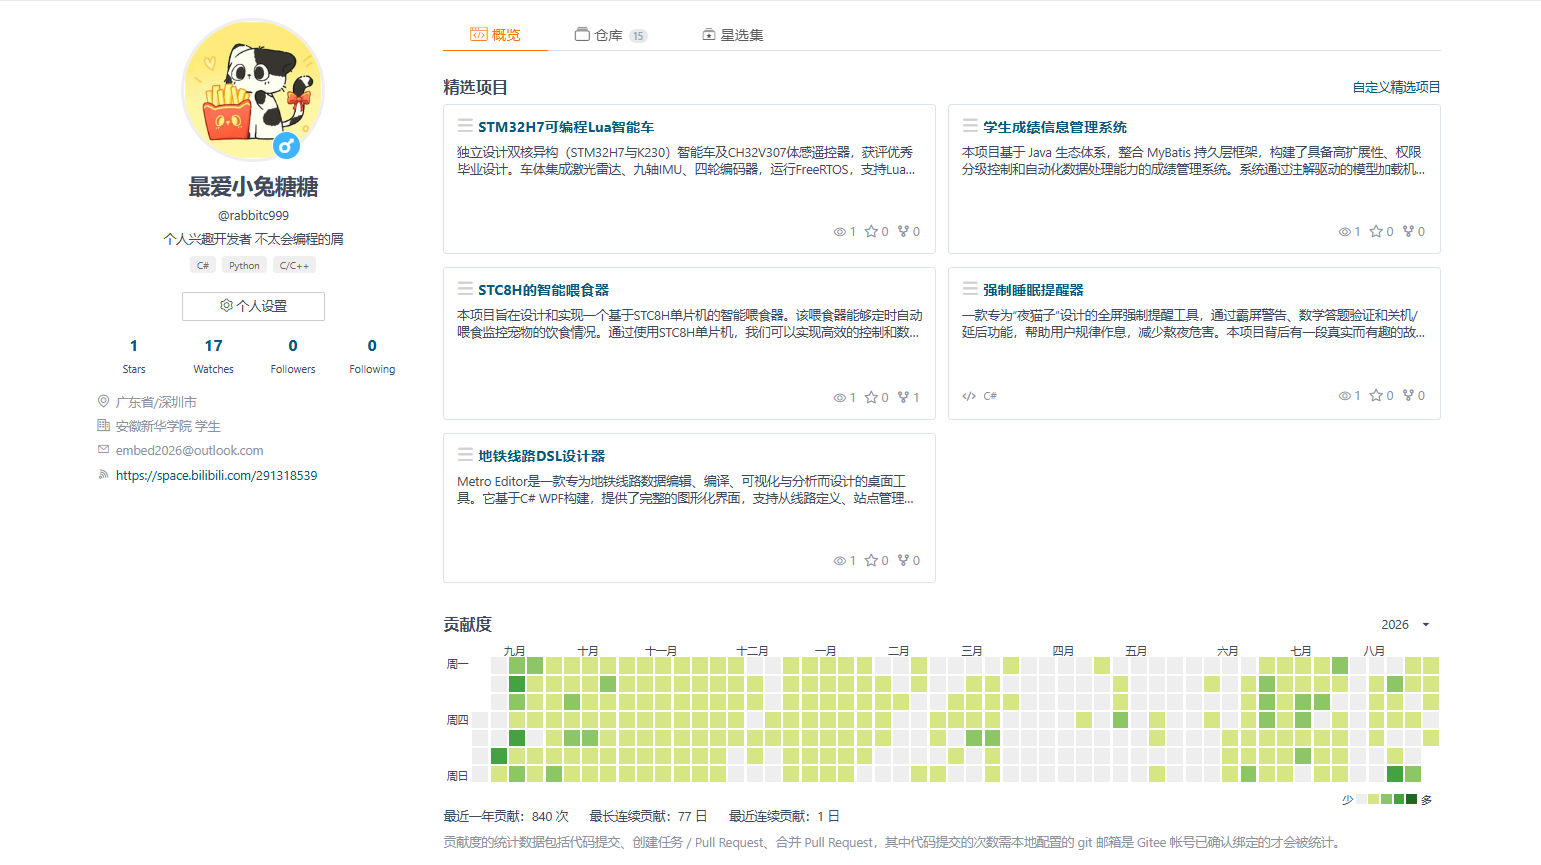
\includegraphics[width=\textwidth]{figure/Gitee.png} \caption{STM32\_PROGRAM 仓库主页} \label{fig:gitee-home}
\end{figure}

% ---------------------------------------------------------------------
\section{如何获取代码}

\subsection{方式一：Git 克隆（推荐）}

在安装了 Git 的电脑上执行：

\begin{lstlisting}
git clone https://gitee.com/rabbitc999/STM32_PROGRAM.git
\end{lstlisting}

克隆后可通过 \texttt{git pull} 获取后续更新。

\subsection{方式二：网页下载 ZIP}

如果不想安装 Git，也可以打开仓库主页，点击页面右上角的“克隆或下载”，选择“下载 ZIP”即可得到当前版本的完整压缩包。

% ---------------------------------------------------------------------
\section{仓库目录结构}

当前仓库主要包含以下几类内容：

\begin{itemize}
\item \texttt{Book/chapters/}：本书全部 \LaTeX{} 章节源码；
\item \texttt{Chapter-embed-basic/} $\sim$ \texttt{Chapter-memory-hardfault/}：按章节整理的示例代码，每章代码目录内部再按小节或功能拆分；
\item \texttt{Book/book.tex}：主文档，按顺序引入全部章节；
\item \texttt{AGENTS.md}：仓库代码规范，AI 协作开发时自动遵守；
\item \texttt{README.md} 与 \texttt{LICENSE}：仓库说明与开源协议。
\end{itemize}

其中：

\begin{itemize}
\item PC 上可直接编译的示例通常附带 \texttt{main.c} 与头文件，可使用 GCC 验证；
\item Keil 与 STM32CubeIDE 工程会保留完整的 \texttt{Project/Hardware/System} 目录；
\item 需要硬件环境的代码会在章节或 README 中标注“Untested，也称待实测”。
\end{itemize}

% ---------------------------------------------------------------------
\section{如何根据章节查找代码}

查找代码时建议按“章节主题”定位：

\begin{enumerate}
\item 先在仓库顶层找到与章节同名的 \texttt{Chapter-*} 目录；
\item 若代码目录名与章节小节名不一致，以目录内 \texttt{README.md} 或源码注释为准。
\end{enumerate}

% ---------------------------------------------------------------------
\section{代码协议与使用说明}

本教程的 \LaTeX{} 源文件与示例代码使用 GPL-3.0 协议开源。你可以学习、复制、修改和分发这些内容，但分发修改后的版本时，应同样遵循 GPL-3.0 的约束，并保留原作者版权声明。

使用代码时请注意：

\begin{itemize}
\item 示例代码以教学为目的，作者不保证其在所有硬件上直接可用；
\item 带“Untested”前缀的代码尚未由作者完成板级验证，运行前请先阅读目录说明；
\item 如发现代码缺陷、文档错误或希望交流技术问题，可在 Gitee 仓库提交 Issue。
\end{itemize}

% ---------------------------------------------------------------------
\section{结语}

这本书是作者在实验室、竞赛和毕业设计中积累经验的整理。如果仓库中的代码能帮助你完成一个课程设计、一次比赛或一个正式项目，那它就是有意义的。欢迎在学习和使用过程中提出意见，让这份教程和代码一起变得更好。

\chapter{作者项目纪实} \label{app:author-projects}

本书正文中的每一段代码、每一个设计模式、每一次“塑料轮子”决策，都来自作者在真实项目中踩过的坑、烧过的板子和熬过的夜。本附录把那些散落在各章的项目片段重新串起来，形成一个完整的技术成长轨迹——从小学的机器人兴趣班，到大学的竞赛和毕业设计，再到工作后的产品开发。如果你在读正文时好奇“这些方案到底能不能跑”，本附录就是答案。

注：除了早期项目，本附录的项目都可以从我的Gitee仓库（\url{https://gitee.com/rabbitc999}）获取。

\section{为什么要有这个附录}

书中正文的目标是“把每个知识点讲清楚”，因此每个例子都被裁剪到刚好说明原理的程度。但真实的项目从来不按教材的章节组织——它同时存在串口、菜单、PID、内存池、硬故障和交期压力，所有这些东西纠缠在一起，才是“嵌入式开发”的真实面目。

本附录按时间线组织，展示作者在不同阶段做过的项目。每个项目都标注了“与正文的对应关系”，方便读者在阅读正文时回查。附录末尾列出了本书配套代码的完整仓库地址，供读者下载和验证。


\section{校园阶段：从入门到竞赛}


\subsection{基于STC8H的智能小车（2023年）}

这是作者在大学阶段做的第一个完整项目，目标是参加“挑战杯”安徽省大学生课外学术科技作品竞赛。项目定位是“验证语音控制小车的可行性”，而非追求产品级的稳定性。

\subsubsection{技术栈}

\begin{itemize}
	\item 主控：STC8H8K64U（国产51内核，主频约24MHz）
	\item 语音识别：ASR-ONE语音模块（串口通信，关键词唤醒）
	\item 通信：HC-05蓝牙模块（手机/电脑蓝牙遥控）
	\item 感知：HC-SR04超声波模块（避障）、TCRT5000L五路循迹模块（黑线循迹）
	\item 执行：L298N电机驱动模块、直流减速电机
	\item 显示：I2C OLED 12864显示屏
\end{itemize}

\begin{figure}[htbp]
	\centering
	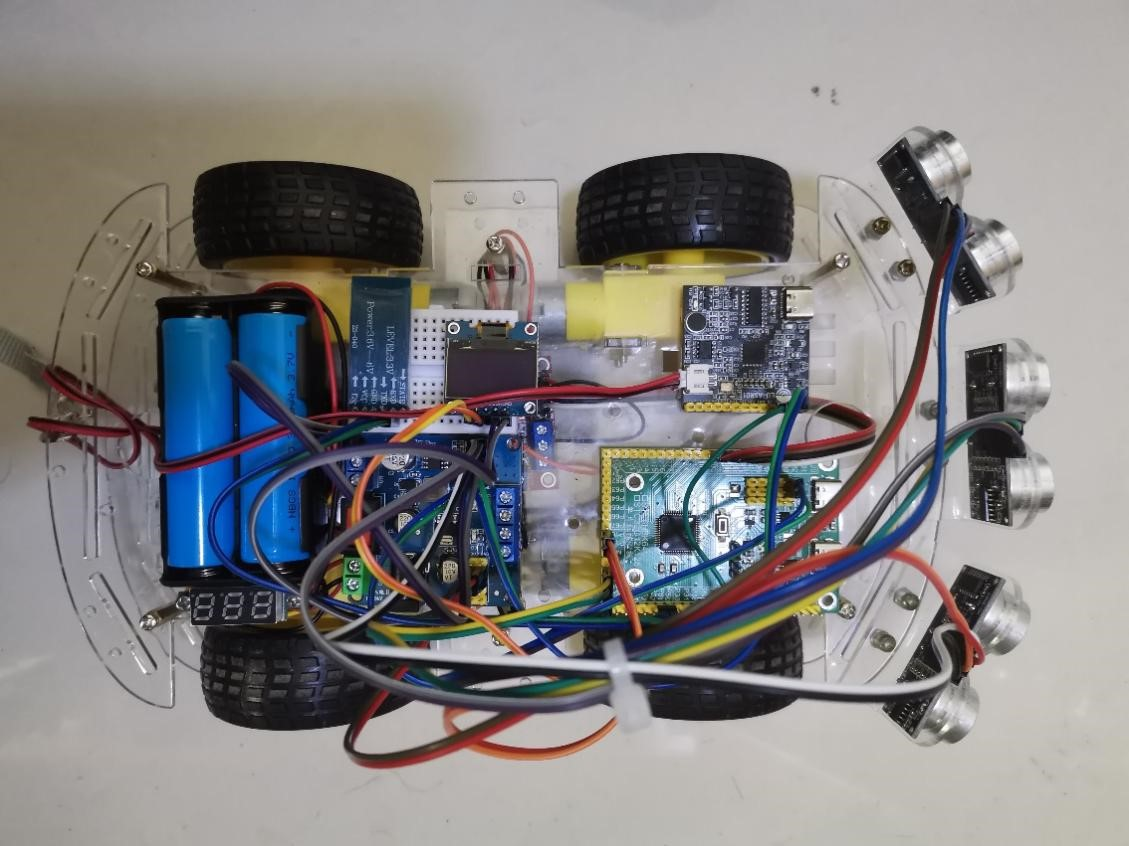
\includegraphics[width=0.5\textwidth]{figure/STC8H-CAR.jpg}
	\caption{基于STC8H的智能小车硬件实物图}
	\label{fig:app-stc8h-hardware}
\end{figure}

\subsubsection{功能与设计}

小车的核心逻辑围绕“模式切换”展开，共三种模式：

\begin{enumerate}
	\item 蓝牙遥控模式：手机或电脑通过蓝牙发送字符指令（'R'/'S'/'T'切换模式，'0'停止，'1'/'2'前进后退，'3'/'4'转向），单片机串口中断接收并执行。
	\item 循迹模式：五路TCRT5000L红外传感器检测黑线位置，输出信号组合决定小车转向方向（左偏则右转，右偏则左转，全在黑线上则直行）。
	\item 超声波避障模式：HC-SR04测距，距离小于阈值时自动转向避开障碍物。
\end{enumerate}

语音模块ASR-ONE通过串口发送指令，与蓝牙共用同一套模式切换逻辑。语音唤醒词为“糖果”，唤醒后可说出“遥控模式”“循迹模式”“避障模式”切换状态。

\subsubsection{代码结构}

项目代码共约800行C语言，核心结构如下：

\begin{itemize}
	\item 主循环：轮询蓝牙串口接收标志和超声波测距，主函数仅约20行；
	\item Motor.c：PWM调速（STC8H的PCA模块）、前进/后退/转向/停止函数；
	\item FollowLine.c：五路循迹传感器的读取与转向决策；
	\item Ultrasonic.c：超声波触发测距与距离计算；
	\item OLED.c：I2C驱动与汉字取模显示（显示项目名称和制作者信息）。
\end{itemize}

串口接收采用中断方式，UART3接收到数据后置标志位，主循环根据标志位执行对应动作。这和第~\ref{ch:scheduler-and-state-machine}~章“标志位法”的调度思想一脉相承——只是当时作者还没意识到这叫做“非阻塞编程”。

\subsubsection{成果与反思}

项目获得了省级奖项，但更重要的是让作者第一次完整经历了“需求分析 → 硬件选型 → 电路焊接 → 软件调试 → 联调测试”的全流程。几个关键教训如下：

\begin{enumerate}
	\item 语音模块在嘈杂环境下识别率下降明显，竞赛现场需要靠近麦克风才能唤醒；
	\item L298N模块发热严重，长时间运行后PWM输出不稳定，小车速度忽快忽慢；
	\item STC8H的RAM只有约8KB，不敢用任何动态内存分配，所有数组都静态定义——这也直接影响了作者后来对第~\ref{ch:memory-alloc}~章“静态内存池”的偏好。
\end{enumerate}

这个项目的代码风格还很稚嫩（所有逻辑堆在main.c里、几乎没有模块化），但它为作者后来的工程习惯奠定了基础：先跑通、再优化、交期优先。


\subsection{STC51温控系统（2024年）}

这是作者在大学课程设计期间完成的项目，硬件基于STC89C52RC单片机（51内核，主频11.0592MHz），核心功能是温度采集、显示、报警与步进电机控制。虽然硬件资源极度有限（RAM约512字节，Flash约64KB），但作者在这个项目里第一次尝试了“菜单框架”的设计，为第~\ref{ch:menu-system}~章的菜单系统提供了最初的灵感。

\subsubsection{技术栈}

\begin{itemize}
	\item 主控：STC89C52RC（经典51单片机）
	\item 温度传感器：DS18B20（单总线数字温度传感器）
	\item 显示：LCD12864（带中文字库，串行/并行可选）
	\item 存储：AT24C02（I2C EEPROM，用于保存参数）
	\item 时钟：DS1302（实时时钟芯片，带备用电池）
	\item 执行：步进电机（28BYJ-48，ULN2003驱动）、蜂鸣器
	\item 输入：4个独立按键
\end{itemize}

\subsubsection{菜单框架设计}

这是项目最核心的部分。LCD12864显示4行，每行可显示8个中文字符或16个英文字符。菜单系统要实现的功能包括：

\begin{enumerate}
	\item 主界面显示：年月日、时分秒、星期、温度（摄氏/华氏/模拟三种模式）；
	\item 子菜单：时间设置、闹钟设置、温度报警阈值设置、步进电机模式设置、历史温度查看；
	\item 参数编辑：选中参数高亮闪烁，按键加减调整，确认保存到EEPROM。
\end{enumerate}

代码结构分为三层：

\begin{itemize}
	\item UI.c：菜单框架核心，维护\texttt{ui\_range\_from}、\texttt{ui\_range\_to}、\texttt{ui\_selected}三个变量控制菜单滚动与选中；
	\item UI\_ClickEvent()：根据选中项分发到不同设置界面（时间/闹钟/温度/步进电机/历史记录）；
	\item 每个设置界面使用状态机管理编辑焦点（select\_set变量），闪烁显示当前正在编辑的字段。
\end{itemize}

菜单项定义为一个二维字符数组：

\begin{lstlisting}[style=c]
	uint8_t code UI_items[ITEM_COUNT][17] = {
		"时间设置",
		"闹钟设置",
		"报警温度设置",
		"步进电机设置",
		"历史温度查看"
	};
\end{lstlisting}

按键处理采用第~\ref{ch:scheduler-and-state-machine}~章介绍的“非阻塞轮询”方式——定时器中断每10ms扫描一次按键状态，主循环通过\texttt{Keys\_GetKey()}读取键值，菜单更新函数根据键值决定操作（进入/退出/上移/下移/确认）。

\subsubsection{EEPROM参数存储}

所有用户可调参数（温度单位模式、闹钟时间、报警阈值、步进电机阈值）都保存在AT24C02中。上电时通过\texttt{Read\_Init()}读取并恢复，修改后通过\texttt{AT\_WriteByte()}或\texttt{AT\_WriteBytes()}立即保存。这和正文第~\ref{ch:param-store}~章介绍的“魔数+结构体整包保存”思路一致——只是当时作者用的是逐字节保存，因为没有定义统一的结构体布局。

\subsubsection{步进电机联动}

步进电机根据温度与阈值的比较结果自动正转或反转：

\begin{itemize}
	\item 模式1（真实温度）：温度高于StepMotorHigh\_C时正转，低于StepMotorLow\_C时反转；
	\item 模式2（模拟温度）：同上，但使用模拟温度值（用于演示，无需传感器）。
\end{itemize}

步进电机驱动在定时器中断中调用\texttt{StepMotor\_Run()}，通过相序数组控制四相绕组依次通电，实现精确的步进角度控制。

\begin{table}[htbp]
	\centering
	\caption{温控系统与正文各章的对应关系}
	\label{tab:app-temp-mapping}
	\begin{tabular}{lll}
		\toprule
		正文章节 & 对应功能 & 项目中的实现 \\
		\midrule
		第~\ref{ch:scheduler-and-state-machine}~章 & 非阻塞调度 & 定时器中断 + 主循环轮询 \\
		第~\ref{ch:menu-system}~章 & 菜单框架 & UI.c中的滚动选择与状态编辑 \\
		第~\ref{ch:param-store}~章 & 参数存储 & AT24C02保存用户配置 \\
		第~\ref{ch:memory-alloc}~章 & 静态内存 & 全部静态分配，无malloc \\
		\bottomrule
	\end{tabular}
\end{table}


\subsection{“挑战杯”RK3588智能车（2025年，未完成）}

这是作者唯一一个“画了饼但没有跑通”的项目，项目的初衷是“用国产RK3588芯片替代NVIDIA Jetson做SLAM导航”，实现从底层控制到上层视觉的完整系统。

\subsubsection{设计目标}

\begin{itemize}
	\item 主控：STM32F407VET6（运动控制）+ 香橙派5MAX（RK3588，8GB内存，6TOPS NPU）
	\item 感知：YDLIDAR X3激光雷达（三角测距，360度扫描）、MPU6050/JY901B陀螺仪
	\item 底盘：麦克纳姆轮四驱（全向移动）
	\item 软件：ROS2 + SLAM建图导航 + AI路径规划
	\item 显示：2.4寸TFT LCD
\end{itemize}

\begin{figure}[htbp]
	\centering
	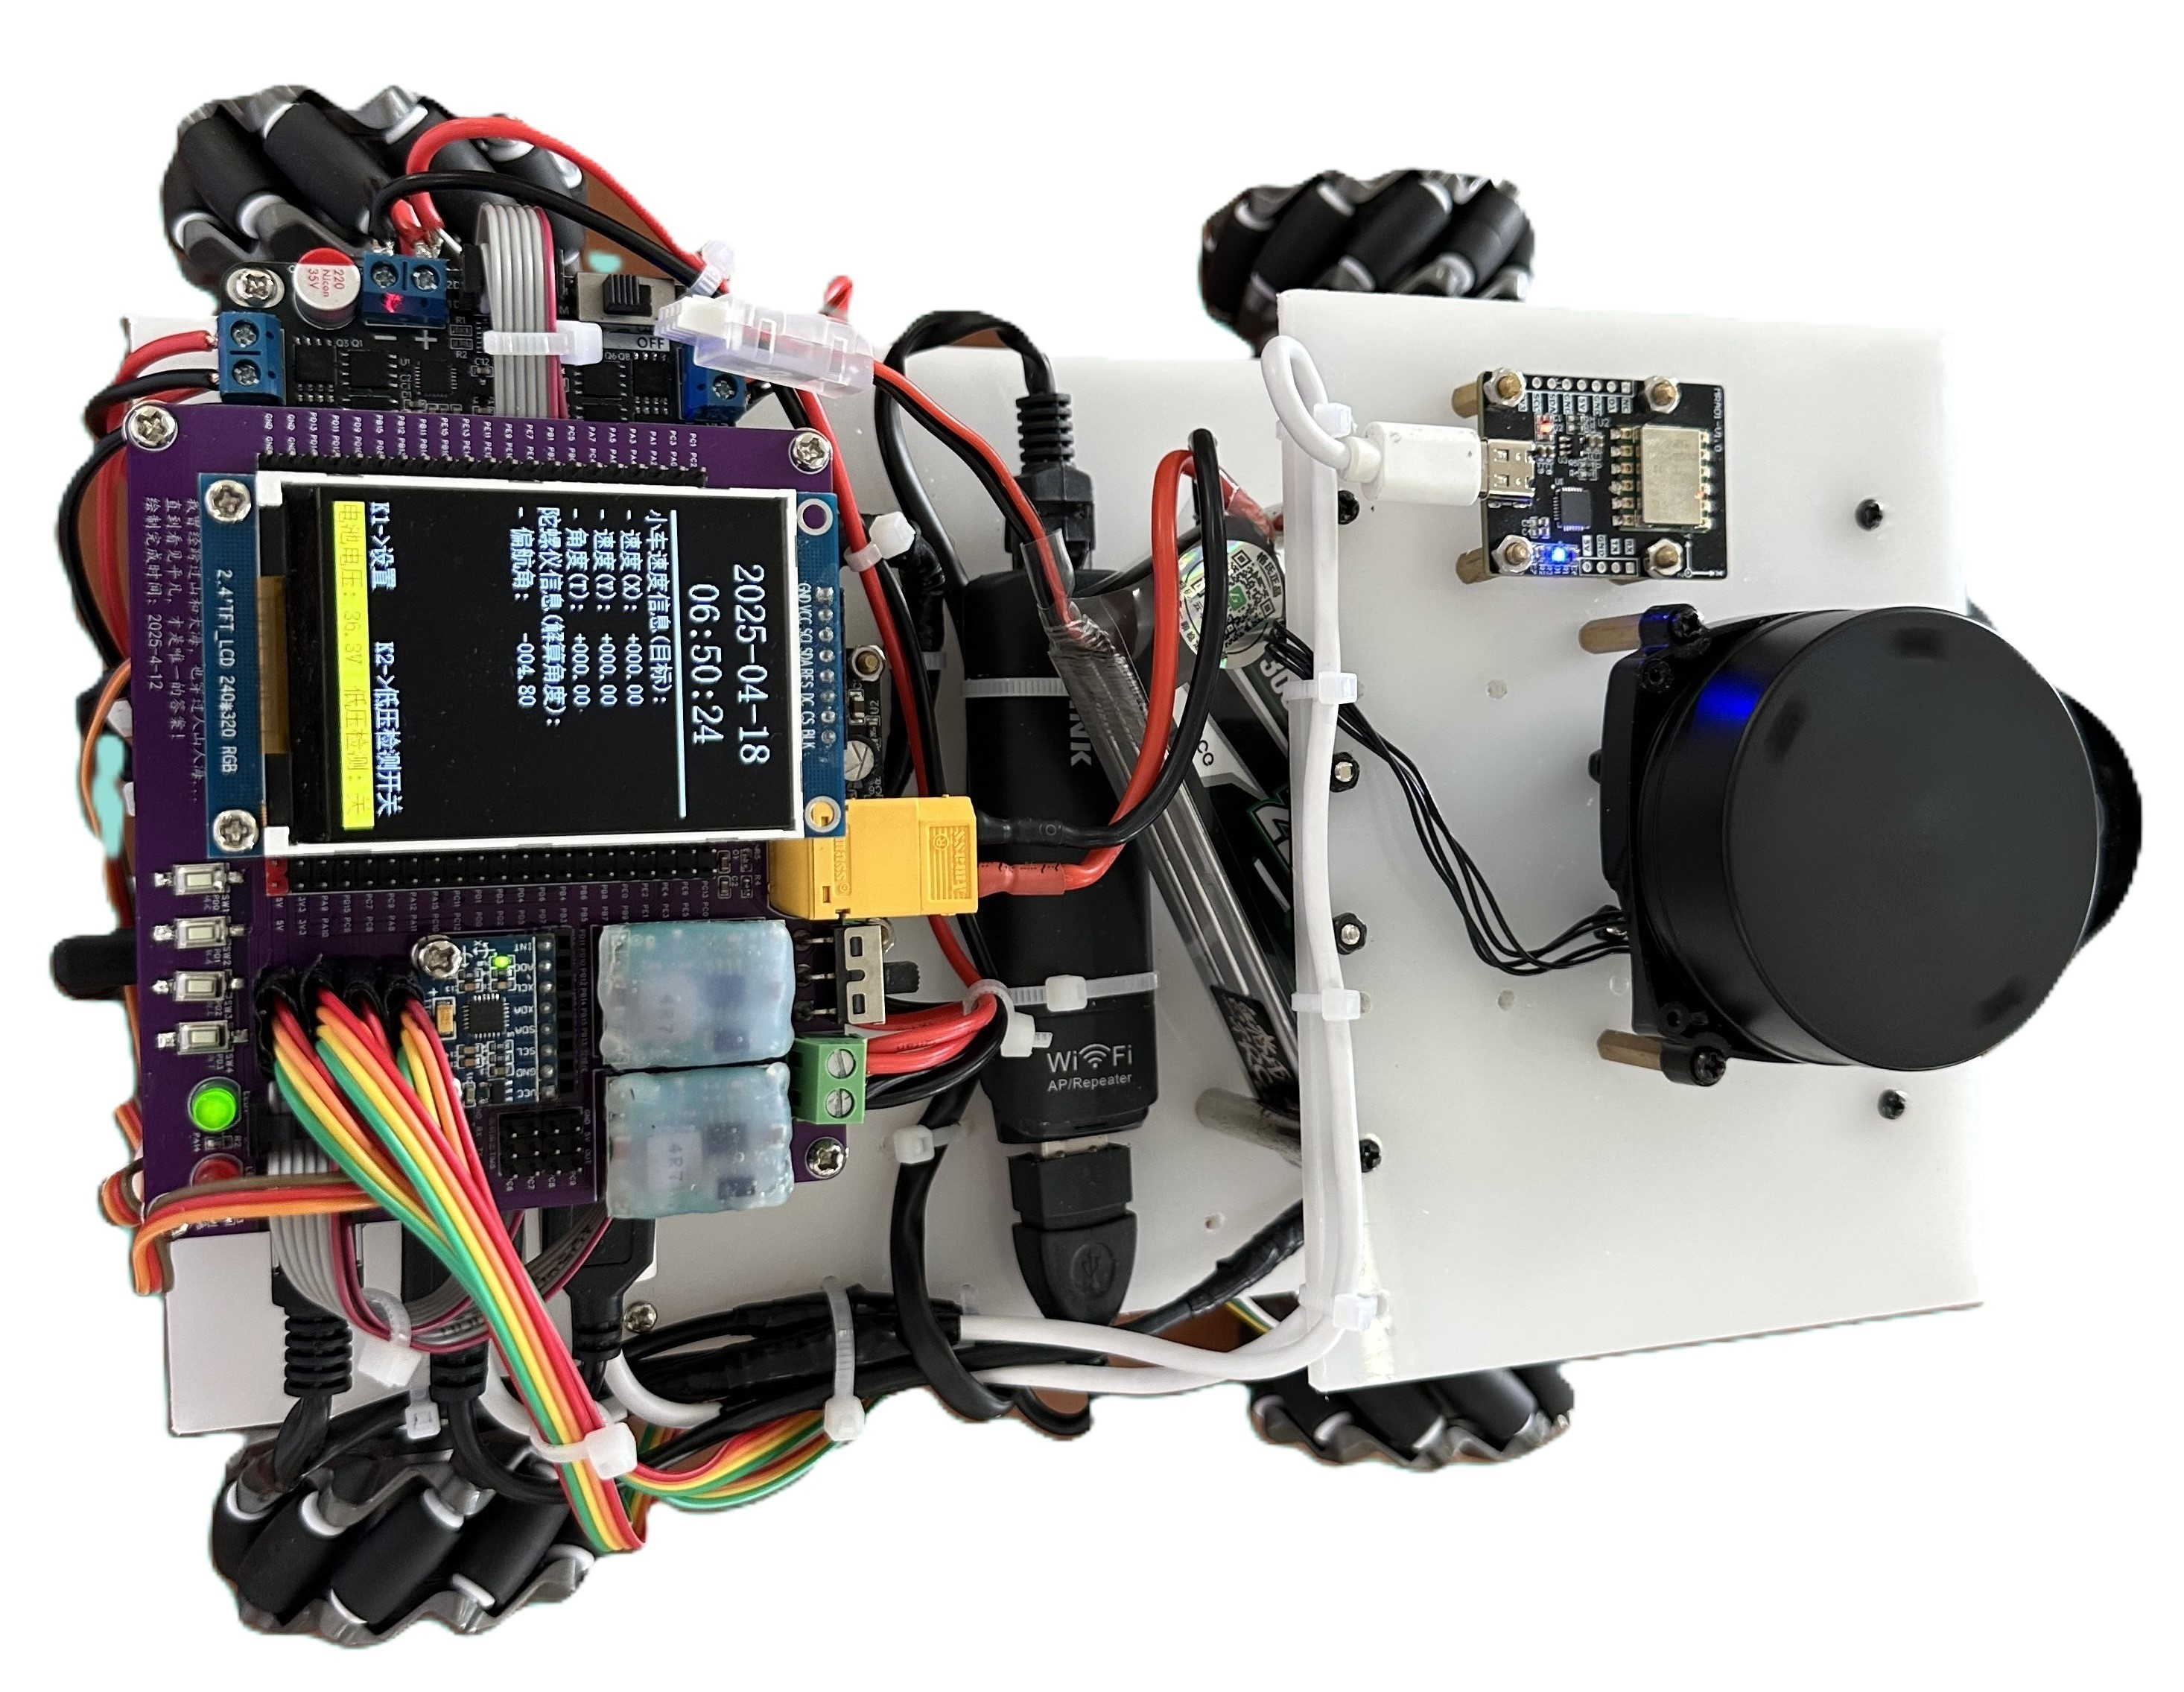
\includegraphics[width=0.5\textwidth]{figure/RK3588-CAR.jpg}
	\caption{RK3588智能车硬件组装图}
	\label{fig:app-rk3588-hardware}
\end{figure}

\subsubsection{为什么没有完成}

项目在硬件层面进展顺利——STM32F407的电机PID控制、串口通信、陀螺仪姿态解算都调通了，激光雷达也能正常输出点云数据。但到了RK3588端的软件集成阶段，项目彻底卡住了。

根本原因只有一个：香橙派是一个“封闭的平台”。

开发者拿到的不是一套可深入的系统，而是一个“黑盒”——官方提供了镜像文件、几个编译好的二进制工具、以及一份超过1000页的PDF文档。但仔细翻看就会发现，这1000页里翻来覆去讲的是同一件事：怎么用镜像烧录工具把系统装进SD卡、怎么用HDMI接显示器看桌面、怎么运行官方预置的几个测试程序（比如NPU推理demo、摄像头采集demo）。至于“系统为什么这样配置”、“驱动是怎么工作的”、“遇到编译错误怎么排查”、“如何把第三方库移植进来”——一个字都没有。

具体到ROS2集成时，问题变成了这样：

\begin{enumerate}
	\item 官方的Ubuntu镜像为了“稳定”，裁剪了大量开发库。安装ROS2需要的依赖时，\texttt{apt}频繁报错说“缺少依赖包”，但这些包的名称在香橙派的镜像源里根本找不到——因为官方源只维护了最基本的系统组件，不维护ROS2相关的包。作者不得不手动从源码编译这些依赖，但编译过程中又发现系统头文件缺失、库版本不匹配、ABI不一致；
	\item 官方提供的NPU推理demo能跑通，但那是“演示级”的代码——它只是告诉你“NPU可以工作”，但没有提供任何关于“如何将自定义模型转换为RKNN格式”的完整文档。作者按照官方文档转换YOLO模型时，转换工具频繁报出“不支持的操作符”错误，而官方论坛上关于这个问题的回复只有一句“请检查模型格式”——然后就没有然后了；
	\item 那份1000页的文档，在作者遇到具体问题时几乎派不上用场。它告诉了你“怎么用”，却没有告诉你“为什么这样用”和“遇到问题怎么办”。作者在论坛上翻到的同类问题，最早的提问时间是一年前，至今没有官方回复。
\end{enumerate}

这个项目最终止步于“能跑但跑不稳”的状态：激光雷达能建图，但地图质量差；电机能控制，但SLAM的定位精度不够；STM32和RK3588能通信，但ROS2节点经常异常退出。作者在截止日期前提交了项目书，但实物演示未能达到预期效果。

这次失败让作者深刻认识到：在嵌入式开发中，“开发板的性能参数”和“开发板的可用性”是两回事。一块开发板的价值，不只取决于它的CPU主频、NPU算力、内存大小，更取决于厂商为开发者提供了多少“可用的信息”——是否开放原理图、是否有完整的驱动源码、是否提供可移植的SDK、是否有活跃的社区和及时的官方支持。如果这些都没有，即便参数再好看，它也只是一块“昂贵的砖头”。

这也是后来毕业设计选择MaixCAM的重要原因之一——MaixCAM的算力只有1TOPS，远不如RK3588的6TOPS，但它的文档是公开的、源码是可读的、社区是活跃的。一个“性能弱但开放”的平台，在交期面前比“性能强但封闭”的平台更可靠。

\subsection{Java 成绩管理系统（2025 年）}

这是作者在大三下学期完成的一组课程设计作品，完成于 2025 年 4 月 5 日。当时同时修了《Java 项目实训》和《Java 热门框架》两门必修课，两门课都要求提交完整的 Web 课程设计，项目内容完全不同。

《Java 项目实训》要求开发一个物流管理系统。这类传统 JSP 框架的项目特点是“能跑，但极其难改”——页面逻辑写在 JSP 里，数据访问层与视图层严重耦合，每新增一个功能模块就要复制粘贴大量重复代码。作者花了一周时间完成这个系统，在开发过程中把数据模型加载、页面组件渲染和功能权限控制三个核心模块从具体业务中剥离出来，形成了一套可复用的框架底座。

随后在《Java 热门框架》课程中，作者需要开发一个学生信息管理系统。他没有从零开始，而是直接将上一项目中抽离出的框架底座套用过来，只需编写新的实体类和页面组装逻辑，就快速完成了第二个功能完整且不重复的系统。

\subsubsection{物流管理系统：开发内容（一周完成）}

物流管理系统采用传统 JSP 框架开发，作者在一周内完成了系统所有功能模块，同时在开发过程中做了以下抽象：

\begin{enumerate}
	\item 模型层抽象：引入 \texttt{@ModelClass} 和 \texttt{@ModelField} 注解，将数据库映射直接写在实体类字段上。\texttt{@ModelField} 的 \texttt{column} 属性被设为必填项，要求显式声明数据库列名，不依赖“驼峰转下划线”的自动推断。
	
	\item 视图层抽象：基于组合模式设计 \texttt{HtmlAtom}、\texttt{HtmlSet}、\texttt{HtmlSingle} 等组件类，将 HTML 页面拆解为可复用的组件树，最终递归渲染为完整页面，替代传统 JSP 中的脚本拼接。
	
	\item 权限层抽象：引入功能码映射表，将“功能 ID → 允许访问的角色列表”集中管理，替代散落在各处的 if-else 判断。
\end{enumerate}

\subsubsection{框架底座：从物流管理系统中剥离}

物流管理系统完成后，作者发现上述三个模块与“物流管理”这个具体业务没有任何绑定关系——它们只依赖实体类上的注解、一个统一的页面渲染接口和一张权限映射表。于是把这三个模块抽成一套独立的框架代码，打包后可以直接导入其他项目使用。

\subsubsection{学生信息管理系统：框架底座的应用}

在《Java 热门框架》课程中，作者直接导入了上一步抽离出的框架底座，只需要做三件事：编写新的实体类（学生、课程、成绩等）并添加注解、组装已有的 HTML 组件形成新页面、配置新的功能码与角色映射关系。整个学生信息管理系统的开发时间大幅缩短，且代码量比从头写减少了约 60\%。

\begin{table}[htbp]
	\centering
	\caption{两个课程设计与正文的对应关系}
	\label{tab:app-java-mapping}
	\begin{tabular}{lll}
		\toprule
		正文章节 & 对应思想 & 本项目中的体现 \\
		\midrule
		第~\ref{ch:script-engine}~章 & 生成器思想 & 注解驱动生成 SQL 与 HTML \\
		第~\ref{ch:command-parser}~章 & 表驱动分发 & 功能码 + 角色映射表控制权限 \\
		第~\ref{ch:menu-system}~章 & 组合模式 UI & HtmlAtom 组件化视图渲染 \\
		\bottomrule
	\end{tabular}
\end{table}

\subsubsection{小结}

这次课程设计的核心不是“写了两个管理系统”，而是：第一个项目用了一周时间完成物流管理系统，在开发过程中抽象出一套可复用的框架底座；第二个项目直接复用底座完成学生信息管理系统，省去了重复劳动。这和本书反复提到的“塑料轮子”逻辑一致——第一次造轮子是为了让项目跑起来，第二次把轮子拆下来装到新车上，是为了不再造第二个轮子。两门必修课最终都顺利通过了验收，而“一次搭建、两次复用”的经历，也让作者在后来设计 MetroEditor 的嵌入式导出模块时，更倾向于思考“哪些东西可以抽成通用骨架”，而不是每次都重新搭一遍地基。

\subsection{基于STM32H743与MaixCAM的双核异构智能小车（2026年）}

这是作者本科阶段最重要的项目，也是本书正文中反复引用的案例。项目的核心决策是：放弃ROS2，用“塑料轮子”方案在交期内交付一个可演示的系统。

\subsubsection{硬件架构}

\begin{itemize}
	\item 主控1：STM32H743XIH6（Cortex-M7，480MHz，1MB RAM，2MB Flash），负责运动控制、传感器融合与底层决策；
	\item 主控2：MaixCAM边缘视觉模块（RISC-V双核，1TOPS NPU），负责YOLOv5s路标识别；
	\item 通信：高速串口（921600bps），自定义HEX帧协议（见第~\ref{ch:serial-fifo}~章）；
	\item 传感器：ICM42688六轴陀螺仪（姿态解算）、镭神N10P激光雷达（TOF，12m测距）、HC-SR04超声波（前后各一）、520霍尔编码器电机（四轮）；
	\item 执行：逐飞科技DRV8701有刷电机驱动模块（×2）、舵机云台（双轴）；
	\item 显示：2.0寸TFT-LCD（240×320，ST7789V2驱动）；
	\item 电源：3S锂电池（11.1V）经TPS5430、RT9013、MP1584多路稳压。
\end{itemize}

\begin{figure}[htbp]
	\centering
	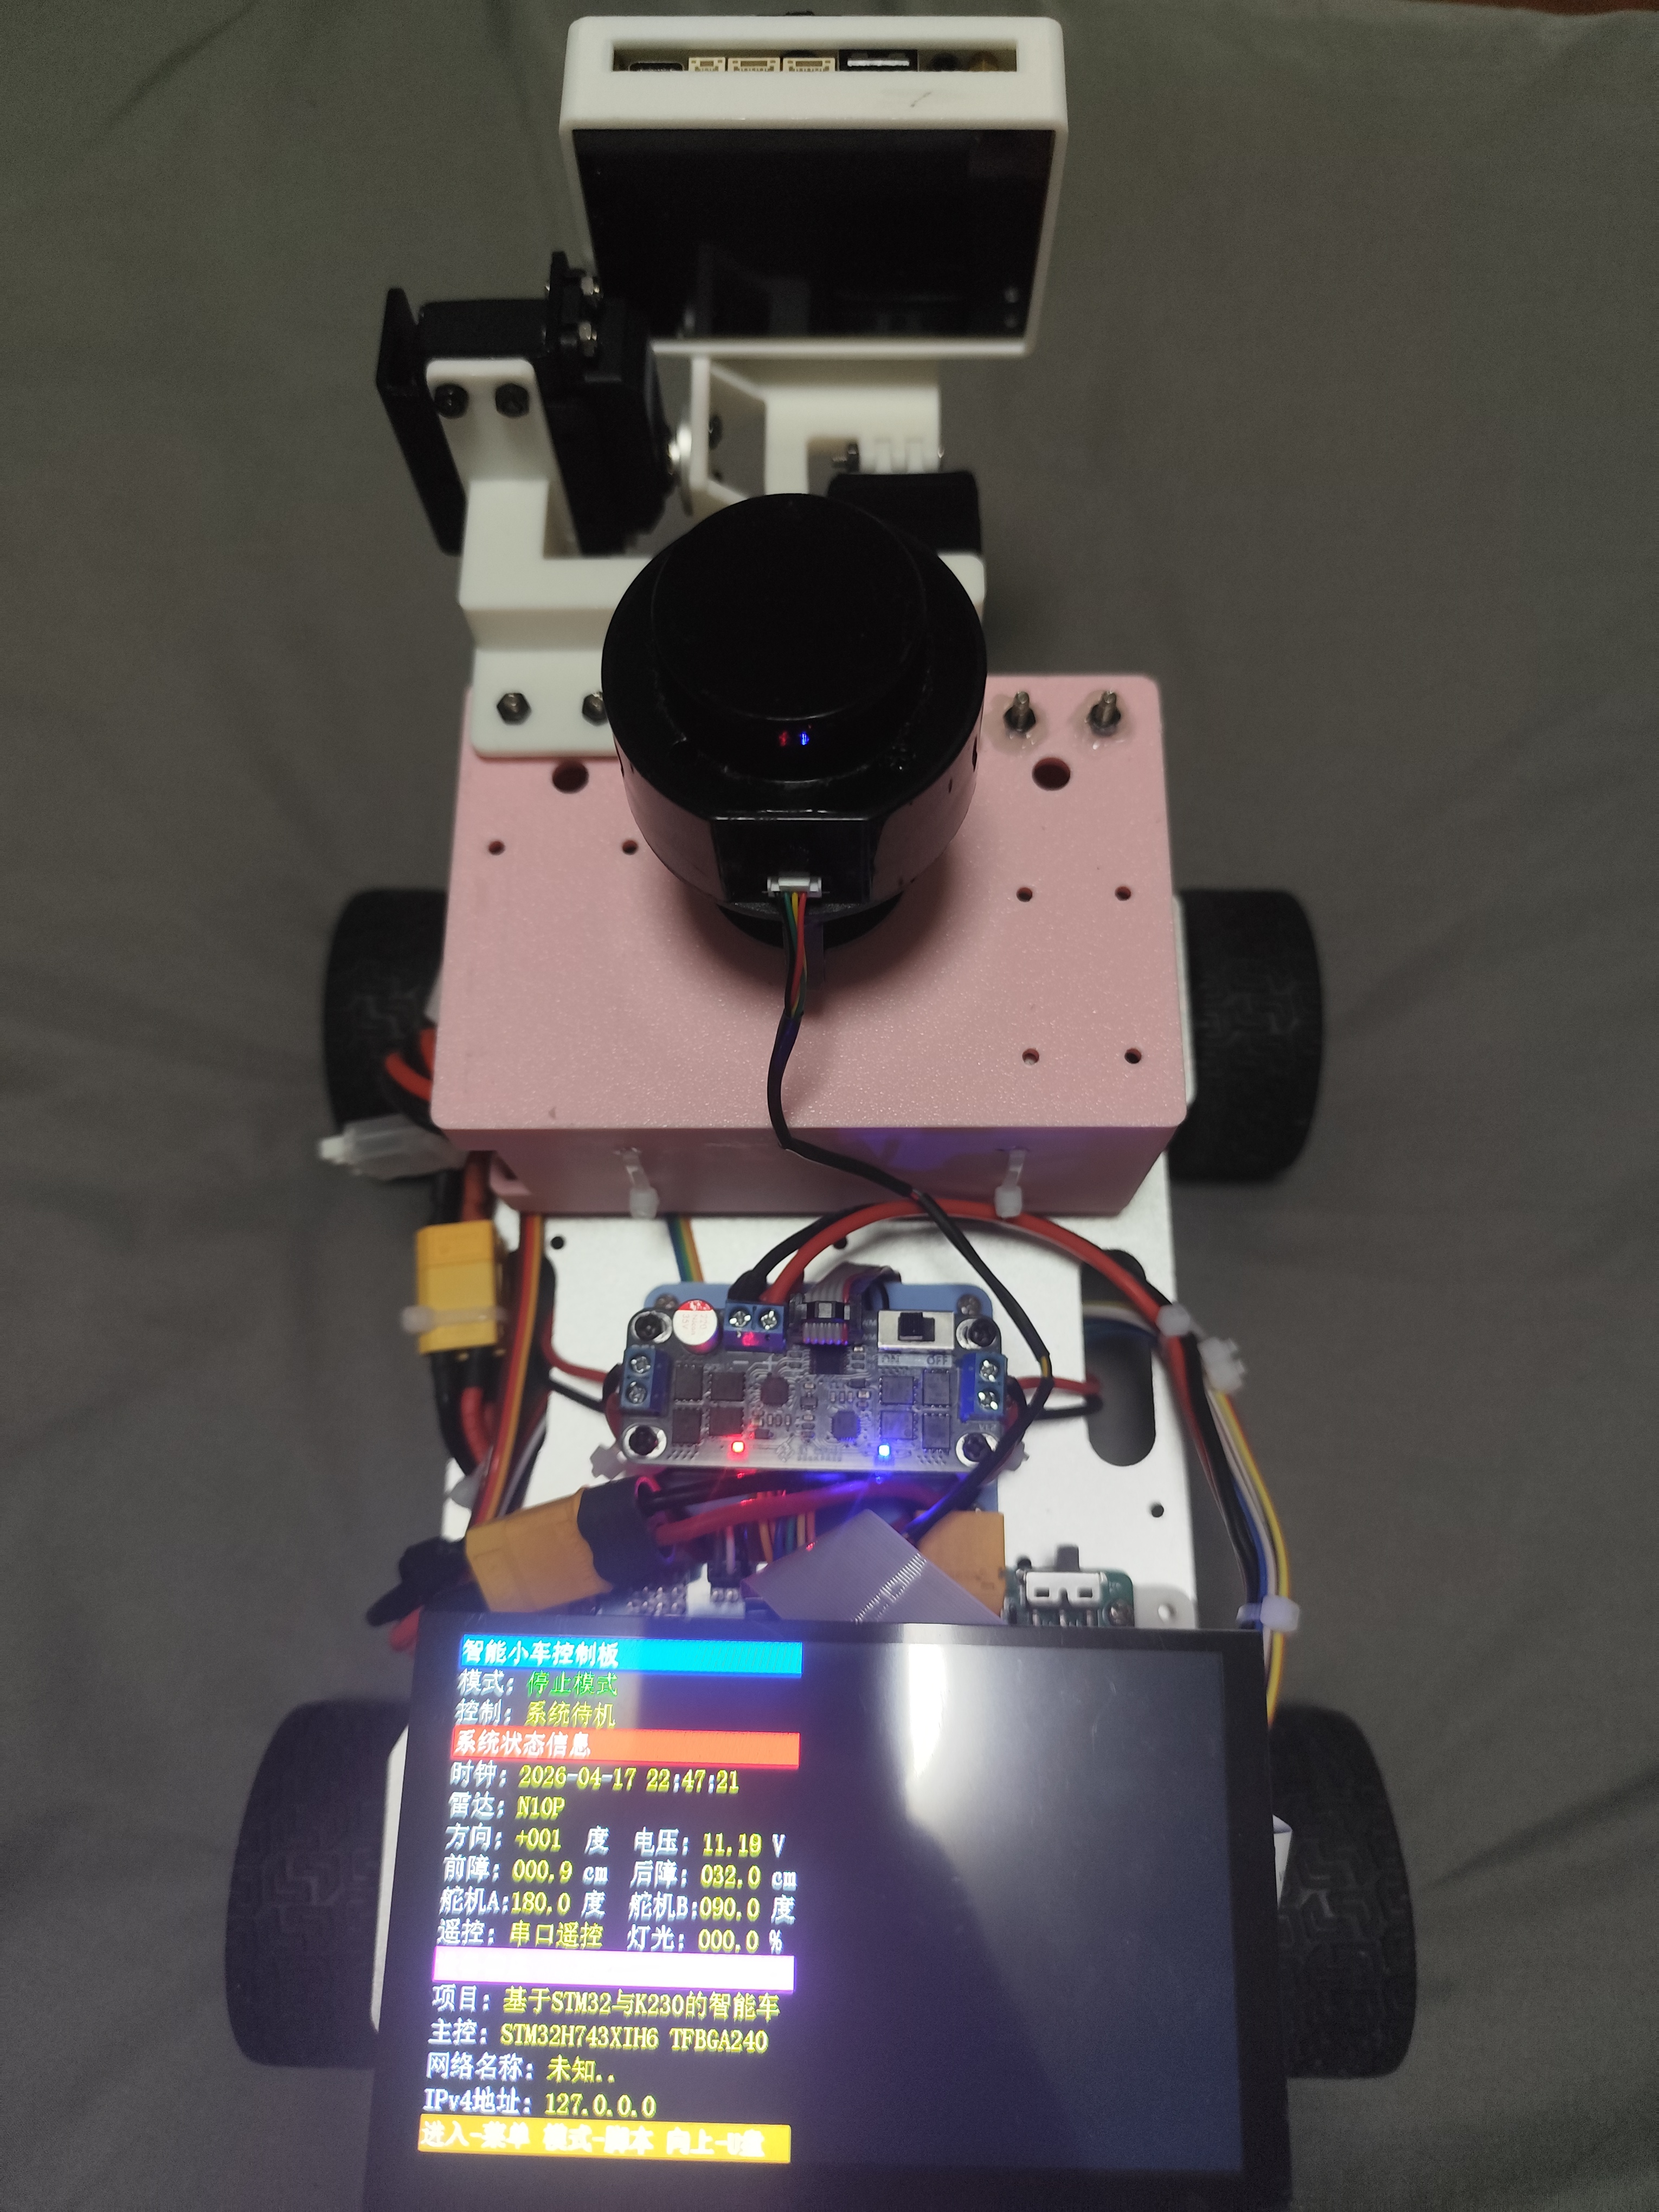
\includegraphics[width=0.5\textwidth]{figure/K230-CAR.jpg}
	\caption{毕业设计智能小车硬件实物图}
	\label{fig:app-graduation-hardware}
\end{figure}

\subsubsection{STM32端软件架构}

系统不依赖RTOS，采用第~\ref{ch:simple-task}~章介绍的\texttt{simple\_task}轻量级协作式调度器。TIM6提供1ms系统节拍，主循环通过\texttt{Task\_Loop()}调度就绪任务；TIM7中断中执行\texttt{Car\_Tick()}，完成电机PID控制等硬实时任务（控制周期1ms）。

主要任务划分如下：

\begin{table}[htbp]
	\centering
	\caption{毕业设计STM32端任务划分}
	\label{tab:app-graduation-tasks}
	\begin{tabular}{lll}
		\toprule
		任务名 & 周期 & 功能 \\
		\midrule
		Main\_Task & 50ms & 系统监控（电池电压、RTC、待机策略） \\
		IMU\_Task & 10ms & ICM42688数据解析、Mahony互补滤波姿态解算、里程计融合 \\
		Lidar\_Task & 100ms & N10P激光雷达数据读取与避障决策 \\
		NRF24L01\_Task & 100ms & 遥控器数据接收与体感指令生成 \\
		Condition\_Task & 100ms & 条件域表达式评估与响应触发 \\
		CS200A\_Task & 20ms & 超声波测距触发、中值滤波 \\
		GUI\_Task & 200ms & TFT-LCD显示（模式、速度、坐标、电池电量）与菜单交互 \\
		Car\_Tick（硬实时） & 1ms & PID控制、编码器读取、电机PWM输出（TIM7中断） \\
		\bottomrule
	\end{tabular}
\end{table}

\subsubsection{自适应里程计融合算法}

这是项目的一个核心创新点，正文第~\ref{ch:about-author}~章有提及，这里补充技术细节。

轮式机器人的里程计在轮胎打滑时会失效——编码器转了很多圈，但小车并没有移动相应距离。传统的EKF（扩展卡尔曼滤波）可以融合IMU和编码器，但其性能依赖精确的系统模型，且需要实时计算雅可比矩阵，在嵌入式平台上计算负载较高。

作者提出的替代方案是：定义“打滑度检测函数”\(P(x,y)\)，根据PID输出量与编码器实测值的比值关系判断打滑程度，然后通过线性加权动态调整编码器和IMU的融合权重。

关键公式如下：

\begin{equation}
	\alpha = \max_{i \in A} P\left(100 \times \frac{v_{i,O}(t_i)}{v_{i,A}(t_i)},\ 100 \times \frac{v_{i,O}(t_{i-1})}{v_{i,A}(t_{i-1})}\right)
\end{equation}

其中\(v_{i,O}\)是PID输出量（期望速度），\(v_{i,A}\)是编码器实测速度。当打滑严重时，\(\alpha\)趋近于1，系统更信任IMU里程计；当打滑轻微时，\(\alpha\)趋近于0，系统更信任编码器里程计。

最终融合公式为：

\begin{equation}
	v_{\text{DOM}}(k+1) = (1-\gamma) \cdot v_{\text{ENC}}(k) + \gamma \cdot v_{\text{IMU}}(k)
\end{equation}

其中\(\gamma = \min\{k_1 \alpha + k_2 \beta + \theta, 1\}\)，\(\beta\)是前后轮间的打滑度，\(\theta\)是固定转换阈值。

测试结果表明，该算法的里程计相对误差最大0.97\%，平均0.46\%，标准差0.24\%，优于纯编码器方案在打滑路面上的表现。

\subsubsection{MaixCAM端视觉推理}

MaixCAM运行MicroPython，通过MaixPy的NN库加载YOLOv5s量化模型（.mud格式）。推理流程如下：

\begin{enumerate}
	\item GC2093摄像头采集图像（640×480），预处理（padding + resize至320×320）；
	\item NPU推理，输出检测框（含坐标、置信度、类别ID）；
	\item 根据类别ID查表（send\_commands字典），通过串口发送对应的条件域指令；
	\item 同时绘制检测框并显示于显示屏。
\end{enumerate}

YOLOv5s模型在自定义路标测试集上的mAP50达到0.995，推理帧率约15FPS，满足实时性要求。

\subsubsection{条件域指令协同机制}

这是STM32与MaixCAM之间“智能协同”的核心——视觉识别结果不是简单地触发固定动作，而是通过条件域指令实现动态决策。

条件域指令格式：

\begin{lstlisting}
	cond set <条件ID> "<表达式>" "<响应动作>" [销毁时间（秒）]
\end{lstlisting}

示例：当检测到类别ID为p14（禁止停车标志）时，发送指令：

\begin{lstlisting}
	cond set 1 "dx>0.2 & abs(dy)<0.5" "t_dyaw:=100-dw" 30
\end{lstlisting}

STM32端解析该指令后，会在30秒内持续监测局部坐标系下的位置增量（dx、dy）和偏航角增量（dw）。当条件满足时，自动执行响应动作（此处为转向修正）。若超时未满足条件，则触发声光报警。

这个机制让系统从“收到指令就执行”升级为“根据实时状态判断是否执行”，是正文第~\ref{ch:script-engine}~章表达式解析器的最直接应用。

\subsubsection{裸机阶段的“四面出击”与失败教训}

在调度器从裸机切换到FreeRTOS之前，作者在裸机框架下尝试过三个“高级功能”——ROS2集成、Lua脚本引擎、RDK X5视觉部署。这三个方向最终都未能成为交付方案的核心，但它们的失败本身构成了毕业设计最重要的经验来源。毕业论文第5.5.4节（ROS2测试）和第5.5.5节（Lua脚本运行）正是这些尝试的历史残留。

\textbf{第一次尝试：ROS2集成（2025年7月—9月）}

作者尝试将小车接入ROS2系统。当时的设想是：STM32作为底层运动控制节点，通过串口与运行ROS2的Linux开发板通信；上位机运行导航、建图等高级功能。硬件选型是香橙派5MAX（RK3588，8GB内存），运行Ubuntu 22.04 + ROS2 Humble。

具体工作包括：在RK3588上编译ROS2的串口通信包（serial）、编写ROS2节点（C++）订阅/cmd\_vel话题将速度指令下发至STM32、STM32端新增ROS2命令解析分支。

三个月的尝试后，项目卡在了以下问题上：ROS2的serial包在ARM架构下编译依赖复杂，串口数据帧偶尔出现粘包和丢包；RK3588的NPU工具链（RKNN）对YOLO模型的支持不完善；ROS2节点启动顺序难以控制（STM32上电即运行，但RK3588需约30秒初始化）。到2025年9月底，作者决定暂时搁置ROS2方向。

\textbf{第二次尝试：Lua脚本引擎移植（2025年10月—11月）}

作者尝试在STM32上移植Lua解释器，目标是让用户可以通过SD卡加载Lua脚本，实现“无需重新编译即可改变小车行为”的可编程能力。

具体工作包括：将eLua移植到STM32H743上（适配静态内存池）、导出C API（Car\_Control、IMU\_GetEuler等注册为Lua模块）、实现SD卡脚本加载功能。

移植工作本身是成功的——Lua解释器能在STM32上运行，示例脚本（小车前进.lua、陀螺仪数据显示.lua）都能正常执行。但Lua解释器占用约40KB Flash和8KB RAM；实时控制任务无法使用解释型语言；用户实际需要的“参数调整”和“行为配置”已被字符串命令系统和FatFS覆盖。最终Lua引擎作为“技术验证”保留在代码仓库中，但默认不编译进交付固件。

\textbf{第三次尝试：RDK X5视觉部署（2026年1月—2月）}

作者尝试将视觉推理从MaixCAM迁移到RDK X5（基于RK3588系，6TOPS算力）。理论上RDK X5能运行更大更精确的模型。

测试结果：YOLOv5n（18ms，mAP50=0.82）、YOLOv5s（35ms，mAP50=0.89）、YOLOv5m（72ms，mAP50=0.91）。

虽然推理速度比MaixCAM更快，但端到端延迟并未显著降低（RDK X5的串口通信栈更复杂）；RDK X5功耗远高于MaixCAM（约5W vs 1.5W）；最关键的是，距离答辩只剩两个月，切换平台的时间成本已超出预算。最终MaixCAM方案被保留为交付方案的核心。

这三个失败的共同点是：作者在项目早期低估了“把一个新技术集成到现有系统中”的边际成本——不仅要让新技术本身跑起来，还要保证它与现有系统的接口稳定、资源不冲突、调试可追踪、维护可持续。

\subsubsection{调度器选型：从裸机到FreeRTOS再到simple\_task}

毕业设计的软件架构经历过一条完整的时间线：裸机（2025年7月—2026年2月）→ FreeRTOS（2026年3月—4月）→ simple\_task（2026年6月）。这不是简单的工具替换，而是一场持续近一年的技术认知升级。

\textbf{第一阶段：裸机（2025年7月—2026年2月）}

项目最初的代码是典型的裸机轮询：一个巨大的\texttt{while(1)}循环里依次调用\texttt{IMU\_Tick()}、\texttt{Car\_Tick()}、\texttt{Key\_Tick()}、\texttt{UI\_Update()}、\texttt{Lidar\_Tick()}，中间穿插着若干个\texttt{Delay\_ms()}。这种写法在项目初期只有三五个功能时还能应付，但到了2025年底，随着激光雷达、超声波、NRF24L01遥控、条件域解析器、GUI菜单、串口命令系统等十多个功能陆续加入，主循环已经臃肿到难以维护的程度。

裸机阶段暴露了三个核心问题：主循环轮询导致周期控制失效（IMU解算需要稳定的10ms周期，但一旦LCD刷新等耗时任务跑久，后续任务都会被推迟）；\texttt{Delay\_ms()}阻塞主循环（有效任务执行时间占比不到30\%）；代码维护困难（一个main.c文件2000多行，改一处可能破坏三个不相关的功能）。

\textbf{第二阶段：FreeRTOS（2026年3月—4月）}

2026年3月初，作者引入了FreeRTOS。拆分的理由非常充分：每个功能模块变成独立任务，通过信号量和队列通信，抢占式调度保证高优先级任务不被低优先级任务拖累。答辩前的两个月里，作者把IMU解算、运动控制、按键扫描、UI刷新、串口解析分别拆成了\texttt{vTask}，并成功让小车跑了起来。

FreeRTOS阶段解决了一些问题：10ms的IMU任务不再被其他任务干扰；任务隔离让代码结构清晰了不少；答辩PPT上可以写“基于FreeRTOS的实时多任务系统”。

但问题也随之出现：任务栈大小难以精确估算（栈溢出的后果是随机HardFault）；抢占式调度引入了新的不确定性（串口FIFO的临界区保护变得更复杂）；FreeRTOS在这个项目里只用了约20\%的功能（任务调度+信号量），却承担了100\%的复杂度和风险。

2026年4月答辩顺利通过。但作者心里清楚，答辩PPT上的FreeRTOS架构图和实际调试中遇到的信号量死锁、栈溢出、任务优先级反转，是两回事。

\textbf{第三阶段：simple\_task（2026年6月，后续复盘）}

答辩结束后，作者重新审视了项目的调度需求：所有任务的执行时间都是微秒级别；任务之间不需要抢占，只需要协作式轮转；周期控制可以用定时器中断统一管理。

于是作者花了半天时间，写了一个只有二百多行的轻量级调度器，后来被正式命名为\texttt{simple\_task}。它的核心逻辑极其简单——定时器中断累加每个任务的\texttt{tickCount}，主循环遍历任务池、执行所有到期任务。任务状态只有四个：WAIT、READY、RUN、DISABLE，状态转换是线性的，没有任何抢占和优先级。

\begin{lstlisting}[style=c]
	/* 简化版 simple_task 核心逻辑 */
	void Task_Tick(void)              /* 1ms 定时器中断调用 */
	{
		for (i = 0; i < TASK_MAX_COUNT; i++) {
			if (task[i].state == WAIT) {
				task[i].tickCount++;
				if (task[i].tickCount >= task[i].period) {
					task[i].state = READY;
				}
			}
		}
	}
	
	void Task_Loop(void)              /* 主循环中调用 */
	{
		for (i = 0; i < TASK_MAX_COUNT; i++) {
			if (task[i].state == READY) {
				task[i].callback();
				task[i].state = WAIT;
				task[i].tickCount = 0;
			}
		}
	}
\end{lstlisting}

这个二百多行的调度器恰好满足了项目的全部需求：任务数量固定、静态分配、不依赖malloc；每行代码都能看懂，单步跟踪时不会跳进黑盒；RAM占用比FreeRTOS方案少了约4KB，Flash少了约15KB；CPU利用率从裸机时期的不足30\%提升到了80\%以上。

有趣的是，\texttt{simple\_task}的雏形早在2026年2月就已经存在——作者当时为了调试某段代码写过一个小型的任务轮询器，但没有正式命名。真正让它成为“调度器”并写进仓库，是答辩后的这次复盘。

一个诚实的注脚：毕业答辩的论文里还保留着FreeRTOS的痕迹，因为那是2026年4月答辩前定稿的。值得说明的是，RTOS 方案仅用于前期的交期验证与流程评审；实际交付的代码库已于 6 月完成迁移，底层调度器切换为第 3 章介绍的 \texttt{simple\_task} 协作式任务调度器。这一调整使系统在保持原有功能完整性的前提下，显著降低了 RAM/ROM 占用，同时消除了抢占式调度带来的执行时序不确定性，提升了长期维护的可靠性。

\subsubsection{成果}

演示视频按时交付，论文答辩顺利通过。系统实现了：

\begin{itemize}
	\item 遥控模式（体感遥控 + NRF24L01无线控制）
	\item 自动避障（激光雷达点云分区 + 超声波辅助）
	\item 航向锁定（Mahony互补滤波姿态解算）
	\item 路标识别触发安全策略（条件域指令）
	\item 里程计定位误差小于2\%
\end{itemize}


\section{职场与业余项目：从功能到产品}


\subsection{SleepReminder——“电子监狱”（2026年）}

这是一个纯软件项目，但它的故事比很多硬件项目更曲折。SleepReminder是一个全屏强制提醒工具，旨在帮助作者自己克服熬夜写代码的习惯。项目的开发过程本身就是一个“与自己较劲”的寓言——作者写了一篇短篇小说《我把自己关进了亲手造的电子监狱》（\texttt{story.pdf}）记录这段经历。

\begin{figure}[htbp]
	\centering
	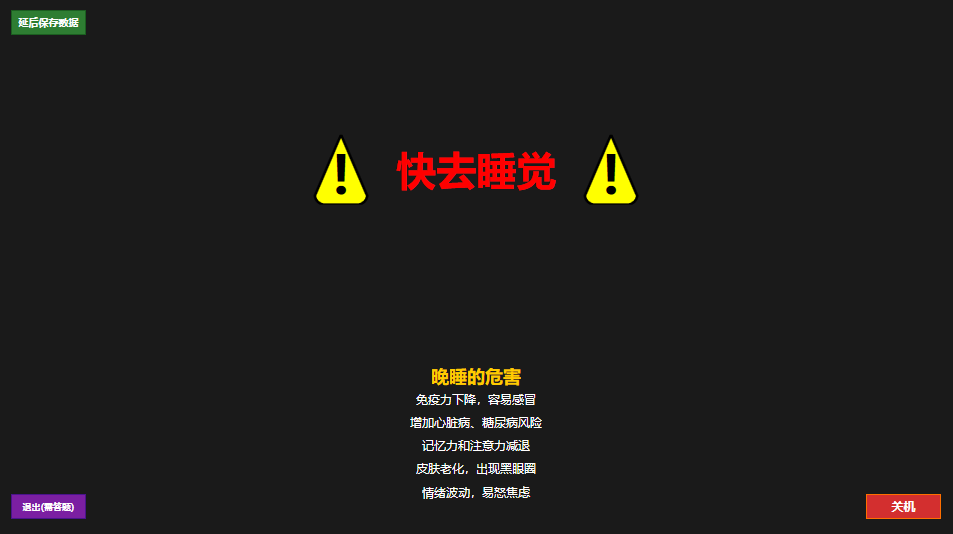
\includegraphics[width=0.8\textwidth]{figure/SleepRemider.png}
	\caption{SleepReminder界面设计图}
	\label{fig:sleep-remider}
\end{figure}

\subsubsection{技术栈}

\begin{itemize}
	\item 语言：C\#（WPF，.NET Framework 4.6.2）
	\item 系统交互：Windows API（进程管理、窗口枚举、注册表操作）
	\item 自启动：启动文件夹快捷方式（COM IWshRuntimeLibrary）
\end{itemize}

\subsubsection{功能迭代}

项目经历了六个版本的演进：

\begin{enumerate}
	\item V1.0（简单弹窗）：每天23:30弹窗，10分钟后锁屏。作者随手点“稍后”，继续写代码到凌晨。
	\item V2.0（反任务管理器）：用\texttt{EnumWindows}遍历窗口，发现任务管理器就\texttt{PostMessage}退出。作者用\texttt{taskkill /f /im}解决。
	\item V3.0（锁系统工具）：禁用CMD、PowerShell，改注册表。作者因为“好麻烦”而放弃抵抗——第一次“被自己的懒惰拯救”。
	\item V4.0（守护进程）：用C语言写守护进程，每秒检查主程序是否存活，被杀后立即重启。作者花了一个半小时跟自己的守护进程打攻防战，没写一行业务代码。
	\item V5.0（系统服务 + 三层嵌套）：注册为Windows系统服务，三层自我修复（主程序被杀→服务重启→被杀→重启计算机→再被杀→再重启）。CPU占用飙到70\%，作者拔了电源线。
	\item V6.0（BIOS方案，文学夸张）：故事中作者拆了笔记本电脑，热风枪吹下BIOS芯片，在ACPI表中嵌入定时关机逻辑。实际上并未真的焊主板，这个方案的真正意义是让作者意识到“战胜自己太麻烦”才是最终的解决方案。
\end{enumerate}

\subsubsection{与正文的对应关系}

这个故事虽然不涉及嵌入式代码，但它完美诠释了正文第~\ref{ch:deadline-ai}~章的观点——“AI是体力劳工，不是脑力军师”。作者在与自己搏斗的过程中，始终是“决策者”，代码只是执行者。那三层嵌套的守护进程不会自己决定“要不要重启”，它只会忠实地执行作者的意志——而作者需要对抗的，恰恰是自己的意志。


\subsection{地铁线路编辑器 MetroEditor（2026年）}

这是作者毕业后做的第一个完整工程工具项目，也是将毕业设计中积累的系统设计能力迁移到纯软件领域的尝试。MetroEditor是一个地铁线路数据编辑、编译、可视化与分析工具，配套Android客户端实现地图推送与记录同步。

\subsubsection{技术栈}

\begin{itemize}
	\item 桌面端：C\# WPF（.NET 8），AvalonEdit（语法高亮），OxyPlot（图表），自定义WebView2地图控件
	\item 嵌入式导出：C语言代码生成（\texttt{metro\_parser.h/c} + \texttt{metro\_data.h}），大端序二进制（.bin）
	\item 移动端：Java（Android 12+），TCP/UDP局域网同步
	\item 路径规划引擎：改进的Dijkstra多目标搜索（距离/换乘/时间/票价/站点数加权）
	\item 物理运行时间计算：基于Davis阻力公式 + 恒功率牵引模型，自适应辛普森积分
\end{itemize}

\begin{figure}[htbp]
	\centering
	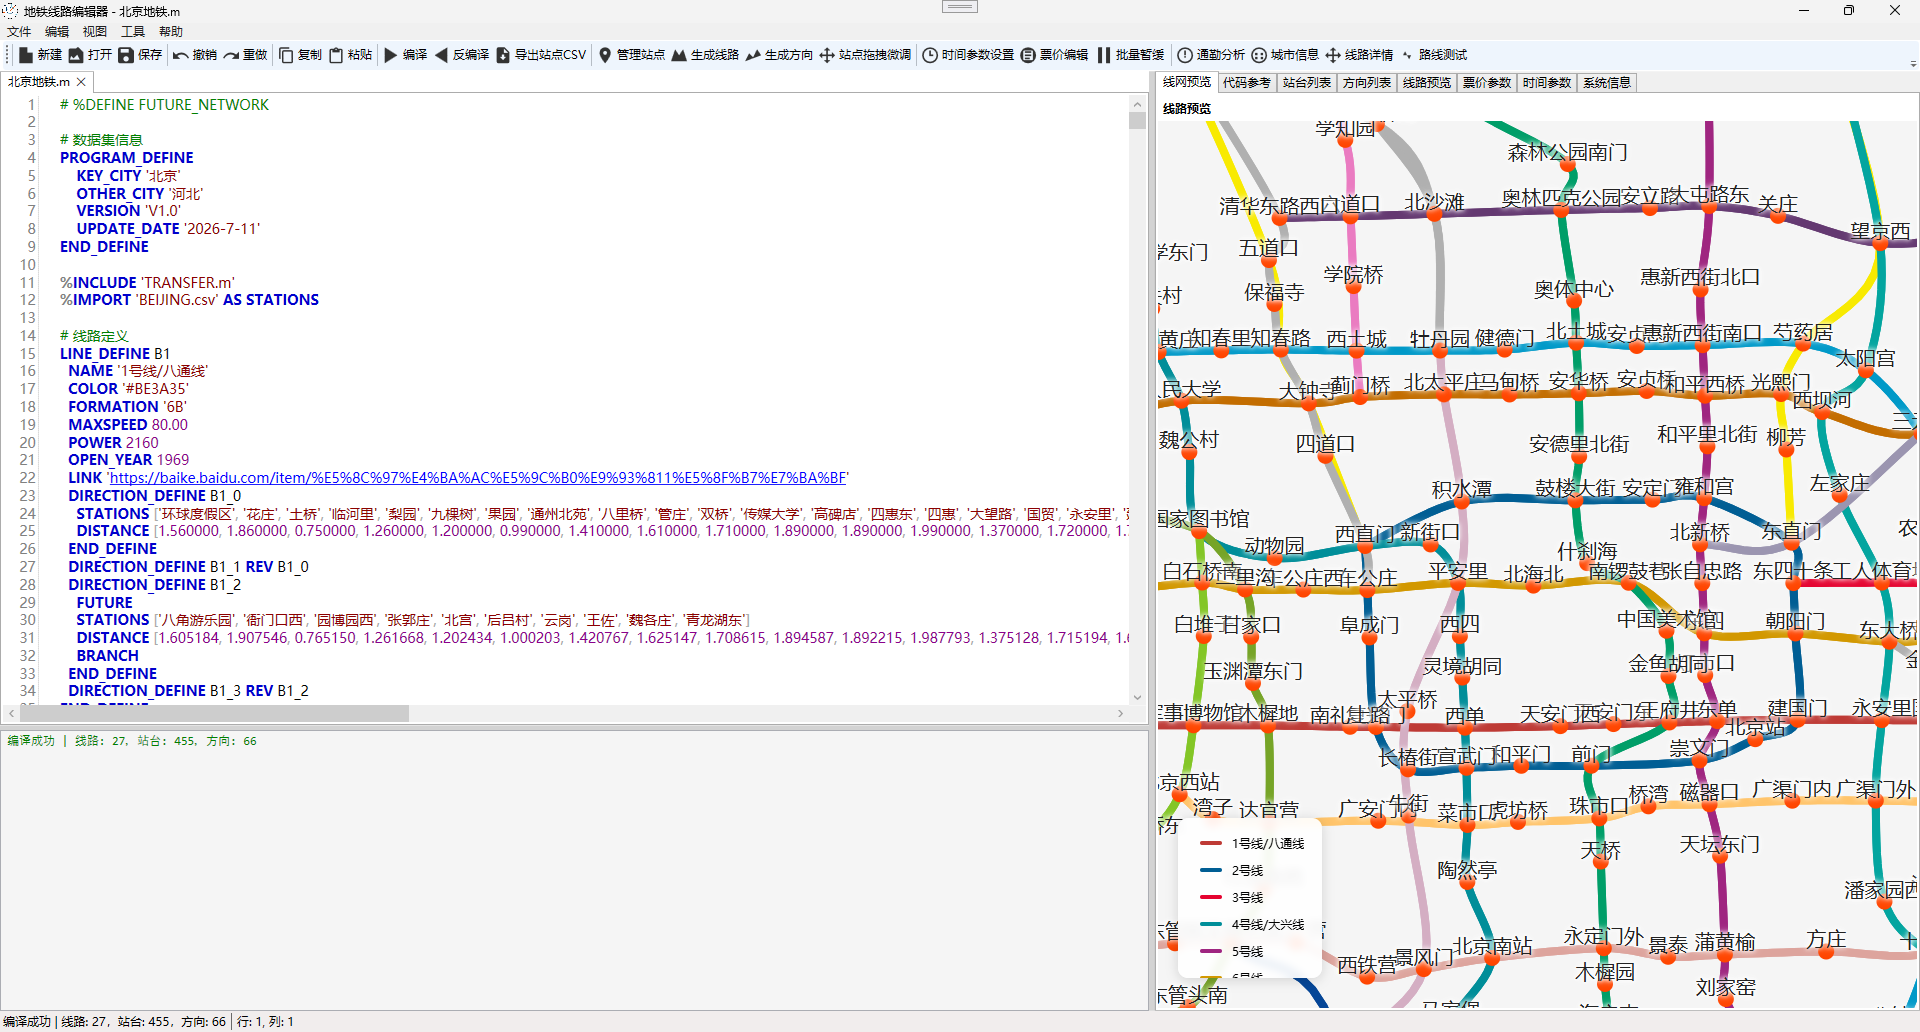
\includegraphics[width=0.8\textwidth]{figure/MetroLang.png}
	\caption{MetroEditor主界面截图（待插入）}
	\label{fig:app-metro-main}
\end{figure}

\subsubsection{核心功能}

\begin{enumerate}
	\item \textbf{MetroLang DSL}：领域特定语言描述地铁网络（站点、线路、方向、票价、换乘、运营参数等）。用户编写\texttt{.metro}文本文件，编译器将其编译为压缩的\texttt{.bmetro}二进制。
	\item \textbf{嵌入式导出}：将路网数据导出为专为资源受限设备设计的\texttt{.bin}二进制格式（零拷贝、大端序），或生成包含完整解析器的C语言代码（\texttt{metro\_parser.h/c} + \texttt{metro\_data.h}），支持多语言站名、预计算区间运行时间，适配STM32/FreeRTOS等平台。
	\item \textbf{通勤分析}：选择起点站，计算到所有站点的最优路径（距离、换乘、时间、票价、痛苦度），支持导出CSV。
	\item \textbf{设备同步}：通过TCP/UDP与Android客户端协同，一键推送地图到手机，实现路线查询、站点打卡、历史行程双向同步。
\end{enumerate}

\subsubsection{嵌入式导出的设计思路}

这是项目最贴近本书主题的部分。地铁线路数据通常包含数百个站点、数千个区间、复杂的票价规则和换乘信息。在嵌入式设备（如手持刷卡机、站内导引屏）上，不可能运行完整的JSON解析器或数据库引擎。

解决方案是：在PC端完成所有“重计算”，只把“查表”所需的数据结构导出为C代码或二进制：

\begin{itemize}
	\item 站点名称：主名与备用名分离存储，嵌入式端通过语言索引快速获取对应翻译；
	\item 区间运行时间：基于物理模型（编组、功率、限速、制动减速度）在PC端预先算好，嵌入式设备只需做整数加法即可完成路径搜索，无需浮点运算；
	\item 数据结构：强制大端序，支持零拷贝直接映射到结构体，无需解析。
\end{itemize}

导出的C代码示例如下（\texttt{metro\_data.h}）：

\begin{lstlisting}[style=c]
	/* 站点数量 */
	#define METRO_STATION_COUNT 128
	
	/* 站点名称表（支持多语言） */
	extern const char *metro_station_names[METRO_STATION_COUNT][2];
	
	/* 区间运行时间表（预计算，单位：秒） */
	extern const uint16_t metro_travel_time[METRO_STATION_COUNT][METRO_STATION_COUNT];
	
	/* 票价表（单位：分） */
	extern const uint16_t metro_fare[METRO_STATION_COUNT][METRO_STATION_COUNT];
	
	/* Dijkstra路径搜索（纯整数运算） */
	uint16_t metro_find_path(uint8_t start, uint8_t end, uint8_t *path, uint8_t max_depth);
\end{lstlisting}

这种“编译期完成重计算、运行期只查表”的思想，与正文第~\ref{ch:script-engine}~章“Python生成器在PC端完成文法分析，单片机只运行生成的C代码”如出一辙。

\begin{table}[htbp]
	\centering
	\caption{MetroEditor与正文各章的对应关系}
	\label{tab:app-metro-mapping}
	\begin{tabular}{lll}
		\toprule
		正文章节 & 对应功能 & MetroEditor中的实现 \\
		\midrule
		第~\ref{ch:command-parser}~章 & 命令解析 & MetroLang DSL的词法/语法解析器 \\
		第~\ref{ch:script-engine}~章 & 生成器思想 & .metro → C代码/二进制导出 \\
		第~\ref{ch:memory-alloc}~章 & 静态内存布局 & 零拷贝二进制结构体映射 \\
		第~\ref{ch:oop-in-c}~章 & 面向接口 & 嵌入式C解析器的统一API \\
		\bottomrule
	\end{tabular}
\end{table}


\section{塑料轮子哲学：一个贯穿始终的红线}

回顾这些项目，可以发现一条清晰的线索：

\begin{itemize}
	\item STC8H智能小车（2023）：用语音模块加蓝牙遥控，替代更复杂的自主导航方案——功能缩水但能跑；
	\item RK3588挑战杯项目（2025）：试图做“完整系统”，结果烂尾——画饼的代价；
	\item STM32H743+MaixCAM毕业设计（2026）：放弃ROS2，用条件域指令替代完整SLAM——塑料轮子策略的成功；
	\item SleepReminder（2026）：用三层守护进程对抗自己的熬夜冲动——直到发现“战胜自己太麻烦”才是最有效的“塑料轮子”；
	\item MetroEditor（2026）：用PC端重计算换取嵌入式端的轻量查表——一种“文明版”的塑料轮子。
\end{itemize}

作者在第~\ref{ch:about-author}~章里说过：“热爱可以等，交期不等。”这句话的背后，是对“塑料轮子”的深刻理解：它不是在否定更先进的技术方案，而是在承认“在有限的时间、有限的资源、有限的精力下，先交付一个可用的结果，比追求一个完美的方案更重要”。

这个附录里的每一个项目，都是这句话的注脚。

\chapter{各章习题参考答案与提示}

本附录给出各章 `problemset` 习题的参考答案。需要“写代码”的题目只给出核心实现思路，读者可在完整示例工程中找到可直接运行的版本；标为“思考题”的题目没有唯一答案，这里只提供分析角度。

% ---------------------------------------------------------------------
\section{第~\ref{ch:embedded-c}~章 参考答案}

\begin{enumerate}
\item 十进制 173 的二进制为 \texttt{10101101}，八进制为 \texttt{255}，十六进制为 \texttt{AD}。
      8 位补码中 \texttt{-5} 为 \texttt{11111011}。
\item 置位：\texttt{REG |= (1u << 3);}；清零：\texttt{REG \&= \textasciitilde(1u << 3);}
\item 位域适合“多个有名字的小字段”反复读写，可读性好，但位分配顺序由编译器决定；联合体适合“同一块内存不同时刻只保存一种类型”的场景，通常需要额外的类型字段区分当前有效成员。
\item 大端从低地址到高地址为 \texttt{12 34 56 78}，小端为 \texttt{78 56 34 12}。可通过联合体读首字节或用 \texttt{uint8\_t *} 强转指针判断。
\item 函数指针保存的是代码入口地址，且签名必须匹配。示例：
\begin{lstlisting}[style=c]
typedef struct { void (*Init)(void); int (*Read)(void); } Device_T;
\end{lstlisting}
\item \texttt{volatile} 只阻止“访问被优化掉”，不能保证“读-改-写”原子性，也不能约束执行顺序；并发修改共享状态时仍需要关中断或临界区。
\end{enumerate}

% ---------------------------------------------------------------------
\section{第~\ref{ch:scheduler-and-state-machine}~章 参考答案}

\begin{enumerate}
\item 定时器中断负责记录时间与“置唤醒标志”，主循环负责扫描任务并执行回调；中断只做短小工作，避免阻塞其他中断。
\item TCB 至少保存状态、回调指针、下次运行时间、周期和运行标志；增加优先级时可加入 \texttt{priority} 字段，并让就绪队列按优先级排序。
\item 按键状态可拆为：空闲、按下消抖确认、按住、松开确认。消抖阶段只作状态迁移，不立即触发业务，比单纯延时更省 CPU 且能区分短按/长按。
\item 中断与主循环同时修改任务标志会形成数据竞争。\texttt{volatile} 只保证读到最新内存值，写-改-写仍要临时关中断或使用临界区。
\item 就绪队列避免每次主循环都扫描全部任务；本实现用 \texttt{isInMsgQuene} 标志防止同一任务重复入队。
\end{enumerate}

% ---------------------------------------------------------------------
\section{第~\ref{ch:simple-task}~章 参考答案}

\begin{enumerate}
\item \texttt{Task\_Tick} 在中断里推进时间并把到期的任务放入 FIFO；\texttt{Task\_Loop} 在主循环中取出任务并调用任务运行函数 \texttt{Task\_RunTask} 执行。
\item 牺牲一个槽位后，\texttt{头 == 尾} 表示空，\texttt{(尾+1)\%容量 == 头} 表示满，判断无需额外字段；若额外记录长度，生产者与消费者都要更新长度，临界区逻辑更复杂。
\item \texttt{Task\_DelayUntil} 适合固定周期任务，误差不会累积；\texttt{Task\_DelayInterrupt} 适合需要“时间到后立即被唤醒”的定时语义，注意回调不能阻塞。
\item \texttt{volatile} 解决“编译器看不到值会变”的问题；但它不保证原子性。涉及入队、出队等读-改-写时必须关闭定时器中断。
\item 静态任务池在编译期分配，无碎片、无内存耗尽风险，失败模式确定；代价是任务数量上限固定。
\item FIFO 按入队顺序执行同一批到期任务，先到先服务，因此不会出现某个任务长期得不到执行的饿死问题。
\end{enumerate}

% ---------------------------------------------------------------------
\section{第~\ref{ch:serial-fifo}~章 参考答案}

\begin{enumerate}
\item 固定数组被写满后，后续字节会覆盖未读数据或直接被丢弃，例如高波特率下主循环稍慢就丢帧。
\item 三种情况分别为：\texttt{StartIndex != EndIndex}、写入后 \texttt{EndIndex} 追上 \texttt{StartIndex} 的前一个槽位、以及写入区间跨过数组末尾后 \texttt{EndIndex} 回到头部附近。
\item 回绕后 \texttt{EndIndex - StartIndex} 可能为负；先加 \texttt{Size} 再取模可得到正确长度。
\item 入队/出队属于读-改-写，需要临时关闭对应串口中断或用临界区，否则可能同时修改头尾指针。
\item 校验码用于发现传输错误；校验失败应丢弃整帧并从“帧头”重新同步，避免把坏数据当作命令执行。
\item 逐字节中断实时性好但中断频繁；空闲中断适合不定长接收；DMA 搬运占用 CPU 最少，但代码与内存复杂度更高。
\end{enumerate}

% ---------------------------------------------------------------------
\section{第~\ref{ch:oop-in-c}~章 参考答案}

\begin{enumerate}
\item 封装的核心是“只暴露稳定接口、隐藏内部实现”，在 C 中通常用不透明结构体指针加模块函数实现。
\item 子结构体把父结构体放在第一个成员，即可通过强转共享父类布局；访问子类字段需还原为子结构体指针。
\item 函数指针表相当于手工虚函数表；新增设备只需实现同一组接口并注册，调用方不需要 \texttt{if/else} 区分类型。
\item 联合体成员共享同一块内存，未写入的成员没有确定值；必须用类型枚举先判断再读取。
\item 面向接口编程把“策略”与“调用方”解耦，例如菜单回调、存储设备读写、显示接口都可用同一套表驱动代码复用。
\end{enumerate}

% ---------------------------------------------------------------------
\section{第~\ref{ch:memory-alloc}~章 参考答案}

\begin{enumerate}
\item 典型布局从低地址到高地址依次是：.data/.bss、堆向上增长、栈向下增长；栈与堆在中间碰撞会互相覆盖导致系统崩溃。
\item \texttt{malloc/free} 时间不确定、易产生碎片、失败时缺少明确恢复路径；固定块池把所有块大小统一，释放后可直接复用，不会产生外部碎片。
\item 可给每块分配一位：\texttt{0} 表示空闲、\texttt{1} 表示占用；扫描字/字节中的位即可快速找到空块。
\item Cortex-M 的非对齐 \texttt{LDR/STR} 可能触发 UsageFault 并升级为 HardFault；因此结构体大小与指针地址都要按成员最大对齐要求处理。
\item 4 字节拷贝利用机器字长，搬运同样字节数所需循环次数更少；源与目标重叠时应改用类似 \texttt{memmove} 的逐字节安全拷贝。
\item 用多个不同块大小的池，申请时按大小选择最接近的池，既能覆盖多种尺寸又不会浪费整块内存。
\end{enumerate}

% ---------------------------------------------------------------------
\section{第~\ref{ch:param-store}~章 参考答案}

\begin{enumerate}
\item 魔数用于识别“这一块数据是否属于本参数结构体”，能发现写错版本或误读其他存储区；校验和只能发现位错误。
\item 常见策略：读取后按版本号补默认字段再写回，或使用 \texttt{schema\_v1/schema\_v2} 迁移工具生成“旧结构体到新结构体”的转换代码。
\item 分组保存可只写发生变化的参数组，减少 Flash 擦写次数，也能隔离“某组损坏”对整块参数的影响；代价是需要在每组带独立校验与版本信息。
\item 文件系统便于电脑导出/导入；二进制体积小、解析快；\texttt{json/yaml} 可读性好但解析开销大，适合 PC 工具或配置量小的场合。
\item Python 脚本、第三方库和文本处理能力强，适合写“读旧文件→转换→生成 C 迁移函数”的一次性工具，且不必占用单片机 Flash。
\end{enumerate}

% ---------------------------------------------------------------------
\section{第~\ref{ch:menu-system}~章 参考答案}

\begin{enumerate}
\item 菜单项中有一个“项类型”枚举（跳转/函数/数值/单选/多选），运行时先判断类型，再读取联合体对应成员。
\item 静态创建把内存峰值限制在编译期，避免运行期碎片；若分配越界，应触发断言或返回错误码，绝不能静默覆盖相邻内存。
\item 页面栈适合“进入子页面再返回”的层级结构，需要记录栈深；显式跳转只需保存当前页面入口，返回目标由调用方显式给出，更适合平级页面。
\item 不填充背景直接绘制文字会残留上一帧的笔画；先清区域再绘制才能保证字符不重叠。
\item 把 LCD 底层 API 隔离到移植层后，菜单核心在 PC 与单片机上使用同一份代码，可先在 PC 验证逻辑再搬硬件。
\end{enumerate}

% ---------------------------------------------------------------------
\section{第~\ref{ch:command-parser}~章 参考答案}

\begin{enumerate}
\item 切词时可用引号或转义表示字符串参数；例如把 \texttt{"hello world"} 作为一个整体 token。
\item 哈希表把字符串比较次数从“逐个命令”降为一次哈希定位；冲突采用线性探测，把后续元素放到下一个空槽。
\item 命令注册表把名字、函数与帮助集中存放，新增命令只需注册一次，主循环和帮助命令都不需要改。
\item \texttt{Param\_T} 内部用类型字段加联合体；\texttt{INT\_PARAM(param, i)} 之类宏先校验类型再按 int 读取。
\item 纯 C 没有反射，无法在运行期按名字自动匹配参数类型；宏可按“类型名展开代码”，C++ 模板可自动生成适配器，本质都是把类型信息放到编译期。
\end{enumerate}

% ---------------------------------------------------------------------
\section{第~\ref{ch:script-engine}~章 参考答案}

\begin{enumerate}
\item 终结符是不可再展开的最小 token；非终结符可被产生式展开；产生式描述展开规则；开始符号是整棵推导树的根。
\item 递归下降用“函数嵌套深度”表达优先级：乘法因子放在 \texttt{ParseFactor}，加减法在上层 \texttt{ParseExpr}，于是 \texttt{*} 先于 \texttt{+} 结合。
\item 直接左递归会让函数无限调用自身；生成器把左递归拆成“先解析基产生式，再循环匹配续产生式”，并在每轮把上一轮结果当作新 \texttt{\$1}。
\item First 集合决定“遇到某个 token 该选哪条产生式”，Follow 集合决定可空产生式何时匹配空；发生冲突时可左因子提取、改写文法或增加向前看。
\item $LR(1)$ 能力最强但表大；$LALR(1)$ 是体积与能力的折中；$LL(1)$ 实现最简单。单片机小资源下通常选择递归下降 $LL(1)$ 或手工解析器。
\item .gram 用逐条 \texttt{lhs := ...} 免去 JSON 嵌套，\texttt{\%var} 可直接声明数组/结构体/字典，动作里写 \texttt{\$1 + \$2} 和 \texttt{int32(0)} 也更接近自然语言。
\end{enumerate}

% ---------------------------------------------------------------------
\section{第~\ref{ch:coroutine-scheduler}~章 参考答案}

\begin{enumerate}
\item \texttt{setjmp} 保存程序计数器、栈指针和 callee-saved 寄存器等现场；\texttt{longjmp} 恢复后，\texttt{setjmp} 之后被修改的“非易失”局部变量值不再保证，应避免依赖。
\item 独立栈保证每个任务挂起时的局部变量都留在自己的栈中；共享栈切换前必须把“本次实际使用过的栈区域”备份，否则会被下一个任务覆盖。
\item 典型迁移：READY 由调度器选中进入 RUNNING；任务调用 \texttt{Task\_Wait} 时保存现场并进入 SUSPEND；时间到或条件满足后被重新置为 READY。
\item 协程把执行到哪一步“藏”在 \texttt{jmp\_buf} 和栈里，代码更接近顺序思维；调试时则难以直接观察“当前在第几行”。
\item 可在栈底填充固定水印值，任务切换或结束时检查水印是否被覆盖，从而得到该任务的最大栈用量。
\item MSP 是主堆栈指针，PSP 是进程堆栈指针；切换任务栈时一般修改 PSP，并在异常返回时由硬件选择对应栈指针。
\end{enumerate}

% ---------------------------------------------------------------------
\section{第~\ref{ch:hardfault}~章 参考答案}

\begin{enumerate}
\item 典型原因包括空指针/野指针解引用、非对齐访问、执行非法函数指针、向无效地址写入等；对应代码示例可在“制造 HardFault”实验中运行。
\item 复位会丢失现场，难以定位；应先保存 LR/PC、栈指针和故障状态寄存器，再决定是离线分析还是复位恢复。
\item CFSR 说明故障类型，BFAR/MMFAR 给出出错地址，LR/PC 帮助定位执行到哪条指令；非法函数指针跳转通常表现为 PC 跳到无意义地址。
\item 非对齐访问是否触发故障与指令类型及配置有关；Cortex-M 可在控制寄存器中开启非对齐访问陷阱，便于尽早发现错误。
\item SEGGER 打印的 R0-R3、R12 是异常前函数参数与临时值，LR/PC 是调用现场，PSR 保存条件标志；结合 \texttt{.map} 文件即可反查故障函数。
\end{enumerate}

% ---------------------------------------------------------------------
\section{第~\ref{ch:linux}~章 参考答案}

\begin{enumerate}
\item \texttt{grep -rni "error" src/ --include="*.c"}
\item \texttt{ps aux | grep python} 找出 python 进程；\texttt{awk '\{print \$2\}'} 提取 PID；\texttt{xargs kill} 把标准输入逐行作为参数传给 \texttt{kill}。
\item 核心逻辑：
\begin{lstlisting}
find /tmp/logs -name "*.log" -mtime +7 -size +1M -exec rm -f {} \;
\end{lstlisting}
\item Makefile 的规则形如“目标:依赖 + 命令”；只要依赖比目标新就会执行命令。头文件也写成依赖后，修改头文件能触发重新编译。
\item \texttt{cmake -S . -B build} 用源码目录 \texttt{.} 生成构建目录 \texttt{build}；再执行 \texttt{cmake --build build} 即可编译运行 \texttt{./build/app}。
\item \texttt{-Wall -Wextra} 打开常见与额外警告，\texttt{-g} 生成调试符号；没有 \texttt{-g} 时调试器无法显示变量与源码行。
\end{enumerate}

\renewcommand\bibname{参考文献}
\begin{thebibliography}{99}
	
\bibitem{aho2006}
Alfred V.~Aho, Monica S.~Lam, Ravi~Sethi, and Jeffrey D.~Ullman.
\newblock {\em Compilers: Principles, Techniques, and Tools},
2nd edition.
\newblock Addison--Wesley, 2006.

\bibitem{yiu2014}
Joseph~Yiu.
\newblock {\em The Definitive Guide to ARM Cortex-M3 and Cortex-M4 Processors},
3rd edition.
\newblock Newnes, 2014.

\bibitem{douglass2011}
Bruce Powel~Douglass.
\newblock {\em Design Patterns for Embedded Systems in C}.
\newblock Elsevier, 2011.

\bibitem{chen2020}
陈海波，夏虞斌等.
\newblock {\em 嵌入式系统设计：CPS与物联网物理世界}.
\newblock 高等教育出版社，2020.

\bibitem{niaoge}
鸟哥.
\newblock {\em 鸟哥的Linux私房菜（基础学习篇）}.
\newblock 人民邮电出版社.

\bibitem{blum2015}
Richard~Blum and Christine~Bresnahan.
\newblock {\em Linux命令行与Shell脚本编程大全}（第3版）.
\newblock 人民邮电出版社，2015.

\bibitem{liuchan}
刘遄.
\newblock {\em Linux就该这么学}.
\newblock 人民邮电出版社.

\bibitem{stevens2013}
W.~Richard~Stevens and Stephen A.~Rago.
\newblock {\em UNIX环境高级编程}（第3版）.
\newblock 人民邮电出版社，2013.

\bibitem{zhuwenwei}
朱文伟，李建英.
\newblock {\em Linux C与C++一线开发实践}.
\newblock 清华大学出版社.

\bibitem{songjingbin}
宋敬彬.
\newblock {\em Linux网络编程}（第2版）.
\newblock 清华大学出版社.

\bibitem{weidongshan}
韦东山.
\newblock {\em 嵌入式Linux应用开发完全手册}.
\newblock 人民邮电出版社.

\bibitem{corbet2005}
Jonathan~Corbet, Alessandro~Rubini, and Greg~Kroah-Hartman.
\newblock {\em Linux设备驱动程序}（第3版）.
\newblock O'Reilly, 2005.

\bibitem{songbaohua}
宋宝华.
\newblock {\em Linux设备驱动开发详解}（第2版）.
\newblock 人民邮电出版社.

\bibitem{madieu}
John~Madieu.
\newblock {\em Linux设备驱动开发}（第2版）.
\newblock 人民邮电出版社.

\bibitem{bovet2005}
Daniel P.~Bovet and Marco~Cesati.
\newblock {\em 深入理解Linux内核}（第3版）.
\newblock 中国电力出版社，2005.

\bibitem{love2010}
Robert~Love.
\newblock {\em Linux内核设计与实现}（原书第3版，典藏版）.
\newblock 机械工业出版社，2010.

\bibitem{jiangyahua}
姜亚华.
\newblock {\em 图解Linux内核：基于6.x}.
\newblock 机械工业出版社，2024.

\bibitem{zhang2026}
最爱小兔糖糖.
\newblock {\em 基于STM32和边缘视觉的智能小车设计与实现}.
\newblock 合肥：安徽新华学院，2026.
	
\end{thebibliography}

\end{document}
